\documentclass[degree=bachelor,language=chinese,tocarialchapter]{thuthesis}
% 选项
%   degree=[bachelor|master|doctor|postdoctor], % 必选,学位类型
%   language=[chinese|english], % 可选(默认:chinese),论文的主要语言
%   secret,                % 可选(默认:关闭),是否有密级
%   tocarialchapter,       % 可选(默认:关闭),章目录中使用黑体(这项表示同时打开下面两项)
%   tocarialchapterentry,  % 可选(默认:关闭),单独控制章标题在目录中使用黑体
%   tocarialchapterpage,   % 可选(默认:关闭),单独控制章页码在目录中使用黑体

% 所有其它可能用到的包都统一放到这里了,可以根据自己的实际添加或者删除。
\usepackage{thuthesis}

% 定义所有的图片文件在 figures 子目录下
\graphicspath{{figures/}}

% ----------------------------------------------------------------------
%           Alphabetical Shortcut Table
% ----------------------------------------------------------------------

\newcommand*\widefbox[1]{\fbox{\hspace{2em}#1\hspace{2em}}}
\newcommand{\xint}{\int_{x_1}^{x_2}}
\newcommand{\tint}{\int_{t_1}^{t_2}}
\newcommand{\mw}{\sqrt{m\omega}}
\newcommand{\de}{\delta}
\newcommand{\dde}{\dot{\delta}}
\newcommand{\di}{\delta_i}
\newcommand{\ddi}{\dot{\delta_i}}
\newcommand{\dddi}{\ddot{\delta_i}}
\newcommand{\dipl}{\delta_{i+1}}
\newcommand{\dimi}{\delta_{i-1}}
\newcommand{\ddt}[1]{\frac{{d} #1}{dt}}
\newcommand{\ddtt}[1]{\frac{d^2 #1}{dt^2}}
\newcommand{\ddx}[1]{\frac{d #1}{dx}}
\newcommand{\ddxx}[1]{\frac{d^2 #1}{dx^2}}
\newcommand{\eps}{\epsilon}
\newcommand{\del}[2]{\frac{\partial #1}{\partial #2}}
\newcommand{\deltwo}[2]{\frac{\partial^2 #1}{\partial #2^2}}
\newcommand{\lam}{\lambda}
\newcommand{\Lam}{\Lambda}
\newcommand{\sig}{\sigma}
\newcommand{\Sig}{\Sigma}
\newcommand{\half}{\frac{1}{2}}
\newcommand{\munu}{{\mu\nu}}
\newcommand{\thalf}{\tfrac{1}{2}}

\newcommand{\bfA}{{\bf A}}
\newcommand{\bfB}{{\bf B}}
\newcommand{\bfC}{{\bf C}}
\newcommand{\bfD}{{\bf D}}
\newcommand{\bfE}{{\bf E}}
\newcommand{\bfF}{{\bf F}}
\newcommand{\bfG}{{\bf G}}
\newcommand{\bfH}{{\bf H}}
\newcommand{\bfI}{{\bf I}}
\newcommand{\bfJ}{{\bf J}}
\newcommand{\bfK}{{\bf K}}
\newcommand{\bfL}{{\bf L}}
\newcommand{\bfM}{{\bf M}}
\newcommand{\bfN}{{\bf N}}
\newcommand{\bfO}{{\bf O}}
\newcommand{\bfP}{{\bf P}}
\newcommand{\bfQ}{{\bf Q}}
\newcommand{\bfR}{{\bf R}}
\newcommand{\bfS}{{\bf S}}
\newcommand{\bfT}{{\bf T}}
\newcommand{\bfU}{{\bf U}}
\newcommand{\bfV}{{\bf V}}
\newcommand{\bfW}{{\bf W}}
\newcommand{\bfX}{{\bf X}}
\newcommand{\bfY}{{\bf Y}}
\newcommand{\bfZ}{{\bf Z}}

\newcommand{\bfa}{{\bf a}}
\newcommand{\bfb}{{\bf b}}
\newcommand{\bfc}{{\bf c}}
\newcommand{\bfd}{{\bf d}}
\newcommand{\bfe}{{\bf e}}
\newcommand{\bff}{{\bf f}}
\newcommand{\bfg}{{\bf g}}
\newcommand{\bfh}{{\bf h}}
\newcommand{\bfi}{{\bf i}}
\newcommand{\bfj}{{\bf j}}
\newcommand{\bfk}{{\bf k}}
\newcommand{\bfl}{{\bf l}}
\newcommand{\bfm}{{\bf m}}
\newcommand{\bfn}{{\bf n}}
\newcommand{\bfo}{{\bf o}}
\newcommand{\bfp}{{\bf p}}
\newcommand{\bfq}{{\bf q}}
\newcommand{\bfr}{{\bf r}}
\newcommand{\bfs}{{\bf s}}
\newcommand{\bft}{{\bf t}}
\newcommand{\bfu}{{\bf u}}
\newcommand{\bfv}{{\bf v}}
\newcommand{\bfw}{{\bf w}}
\newcommand{\bfx}{{\bf x}}
\newcommand{\bfy}{{\bf y}}
\newcommand{\bfz}{{\bf z}}

\newcommand{\mcA}{{\mathcal{A}}}
\newcommand{\mcB}{{\mathcal{B}}}
\newcommand{\mcC}{{\mathcal{C}}}
\newcommand{\mcD}{{\mathcal{D}}}
\newcommand{\mcE}{{\mathcal{E}}}
\newcommand{\mcF}{{\mathcal{F}}}
\newcommand{\mcG}{{\mathcal{G}}}
\newcommand{\mcH}{{\mathcal{H}}}
\newcommand{\mcI}{{\mathcal{I}}}
\newcommand{\mcJ}{{\mathcal{J}}}
\newcommand{\mcK}{{\mathcal{K}}}
\newcommand{\mcL}{{\mathcal{L}}}
\newcommand{\mcM}{{\mathcal{M}}}
\newcommand{\mcN}{{\mathcal{N}}}
\newcommand{\mcO}{{\mathcal{O}}}
\newcommand{\mcP}{{\mathcal{P}}}
\newcommand{\mcQ}{{\mathcal{Q}}}
\newcommand{\mcR}{{\mathcal{R}}}
\newcommand{\mcS}{{\mathcal{S}}}
\newcommand{\mcT}{{\mathcal{T}}}
\newcommand{\mcU}{{\mathcal{U}}}
\newcommand{\mcV}{{\mathcal{V}}}
\newcommand{\mcW}{{\mathcal{W}}}
\newcommand{\mcX}{{\mathcal{X}}}
\newcommand{\mcY}{{\mathcal{Y}}}
\newcommand{\mcZ}{{\mathcal{Z}}}

\newcommand{\bbA}{{\mathbb{A}}}
\newcommand{\bbB}{{\mathbb{B}}}
\newcommand{\bbC}{{\mathbb{C}}}
\newcommand{\bbD}{{\mathbb{D}}}
\newcommand{\bbE}{{\mathbb{E}}}
\newcommand{\bbF}{{\mathbb{F}}}
\newcommand{\bbG}{{\mathbb{G}}}
\newcommand{\bbH}{{\mathbb{H}}}
\newcommand{\bbI}{{\mathbb{I}}}
\newcommand{\bbJ}{{\mathbb{J}}}
\newcommand{\bbK}{{\mathbb{K}}}
\newcommand{\bbL}{{\mathbb{L}}}
\newcommand{\bbM}{{\mathbb{M}}}
\newcommand{\bbN}{{\mathbb{N}}}
\newcommand{\bbO}{{\mathbb{O}}}
\newcommand{\bbP}{{\mathbb{P}}}
\newcommand{\bbQ}{{\mathbb{Q}}}
\newcommand{\bbR}{{\mathbb{R}}}
\newcommand{\bbS}{{\mathbb{S}}}
\newcommand{\bbT}{{\mathbb{T}}}
\newcommand{\bbU}{{\mathbb{U}}}
\newcommand{\bbV}{{\mathbb{V}}}
\newcommand{\bbW}{{\mathbb{W}}}
\newcommand{\bbX}{{\mathbb{X}}}
\newcommand{\bbY}{{\mathbb{Y}}}
\newcommand{\bbZ}{{\mathbb{Z}}}

\newcommand{\mfa}{{\mathfrak{a}}}
\newcommand{\mfb}{{\mathfrak{b}}}
\newcommand{\mfc}{{\mathfrak{c}}}
\newcommand{\mfd}{{\mathfrak{d}}}
\newcommand{\mfe}{{\mathfrak{e}}}
\newcommand{\mff}{{\mathfrak{f}}}
\newcommand{\mfg}{{\mathfrak{g}}}
\newcommand{\mfh}{{\mathfrak{h}}}
\newcommand{\mfi}{{\mathfrak{i}}}
\newcommand{\mfj}{{\mathfrak{j}}}
\newcommand{\mfk}{{\mathfrak{k}}}
\newcommand{\mfl}{{\mathfrak{l}}}
\newcommand{\mfm}{{\mathfrak{m}}}
\newcommand{\mfn}{{\mathfrak{n}}}
\newcommand{\mfo}{{\mathfrak{o}}}
\newcommand{\mfp}{{\mathfrak{p}}}
\newcommand{\mfq}{{\mathfrak{q}}}
\newcommand{\mfr}{{\mathfrak{r}}}
\newcommand{\mfs}{{\mathfrak{s}}}
\newcommand{\mft}{{\mathfrak{t}}}
\newcommand{\mfu}{{\mathfrak{u}}}
\newcommand{\mfv}{{\mathfrak{v}}}
\newcommand{\mfw}{{\mathfrak{w}}}
\newcommand{\mfx}{{\mathfrak{x}}}
\newcommand{\mfy}{{\mathfrak{y}}}
\newcommand{\mfz}{{\mathfrak{z}}}

\newcommand{\mfA}{{\mathfrak{A}}}
\newcommand{\mfB}{{\mathfrak{B}}}
\newcommand{\mfC}{{\mathfrak{C}}}
\newcommand{\mfD}{{\mathfrak{D}}}
\newcommand{\mfE}{{\mathfrak{E}}}
\newcommand{\mfF}{{\mathfrak{F}}}
\newcommand{\mfG}{{\mathfrak{G}}}
\newcommand{\mfH}{{\mathfrak{H}}}
\newcommand{\mfI}{{\mathfrak{I}}}
\newcommand{\mfJ}{{\mathfrak{J}}}
\newcommand{\mfK}{{\mathfrak{K}}}
\newcommand{\mfL}{{\mathfrak{L}}}
\newcommand{\mfM}{{\mathfrak{M}}}
\newcommand{\mfN}{{\mathfrak{N}}}
\newcommand{\mfO}{{\mathfrak{O}}}
\newcommand{\mfP}{{\mathfrak{P}}}
\newcommand{\mfQ}{{\mathfrak{Q}}}
\newcommand{\mfR}{{\mathfrak{R}}}
\newcommand{\mfS}{{\mathfrak{S}}}
\newcommand{\mfT}{{\mathfrak{T}}}
\newcommand{\mfU}{{\mathfrak{U}}}
\newcommand{\mfV}{{\mathfrak{V}}}
\newcommand{\mfW}{{\mathfrak{W}}}
\newcommand{\mfX}{{\mathfrak{X}}}
\newcommand{\mfY}{{\mathfrak{Y}}}
\newcommand{\mfZ}{{\mathfrak{Z}}}
\usepackage{xcolor}
\renewcommand{\emph}[1]{\textcolor{purple}{\textit{#1}}} % for emph color

\usepackage{siunitx} % \SI{1.234}{\m\per\square\s} \SI{1e-4}{\metre}
\DeclareSIUnit{\rad}{rad} % \rad is removed frmo siunitx 2 since it is not a SI unit. 

% \usepackage{amsmath}
\newcommand\vect{\mathbf}
% \newcommand\matr{\mathbf} % \matrix is defined in LaTeX2e kernel
% \newcommand\tens{\mathcal}

\usepackage{romannum}  % \Romannum{3} \romannum{3}


\def\degree{${}^{\circ}$} % degree symbols
\sisetup{math-micro=\text{µ},text-micro=µ} 
% Very strange that the micro symbol does not appear in \SI{}{}, 
% this is a bug found at https://tex.stackexchange.com/questions/33965/siunitx-µ-doesnt-work 
\usepackage[super]{nth} % 1st, 2nd, ...


% Conflict with thuthesis
% \usepackage[math-style=ISO]{unicode-math} % XeTeX driver only supports unicode.  (hyperref)  Enabling option `unicode'. 
% Sometimes pasted texts may contain unicode math symbols which may cause compiling errors, the package is capable to help you skip those trivial errors caused by compiling those symbols which used to be uncompilable properly.

\usepackage{etoolbox}
\newbool{isBeamer} 
% \booltrue{isBeamer}
\boolfalse{isBeamer}
% \ifbool{isBeamer}{<true>}{<false>}

\usepackage{booktabs}

\makeatletter
\newcommand{\rmnum}[1]{\romannumeral #1}
\newcommand{\Rmnum}[1]{\expandafter\@slowromancap\romannumeral #1@}
\makeatother
\usepackage{hyperref}


% \usepackage[T1]{fontenc} //This may cause some alignment problem in cover
\usepackage[utf8]{inputenc}


% Special scientist naem 
\usepackage{xspace}
\newcommand{\Poincare}{Poincar\'e\xspace}
\newcommand{\adele}{ad\`ele\xspace}
\newcommand{\Cech}{\v{C}ech\xspace}
\newcommand{\Erdos}{Erd\H{o}s\xspace}
\makeatletter
\newcommand{\etale}{\'etal\@ifstar{\'e}{e\xspace}}
\makeatother


\newcommand{\vE}{\vect{E}}
\newcommand{\vx}{\vect{x}}
\newcommand{\vv}{\vect{v}}
\newcommand{\ftxv}{f(t, \vect{x}, \vect{v})}
\newcommand{\bbRRR}{\bbR^{3}}
\newcommand{\bbRx}{\bbR_{x}^{3}}
\newcommand{\bbRv}{\bbR_{v}^{3}}

% 可以在这里修改配置文件中的定义。导言区可以使用中文。
% \def\myname{薛瑞尼}

\begin{document}

%%% 封面部分
\frontmatter
\thusetup{
  %******************************
  % 注意:
  %   1. 配置里面不要出现空行
  %   2. 不需要的配置信息可以删除
  %******************************
  %
  %=====
  % 秘级
  %=====
  % secretlevel={秘密},
  % secretyear={10},
  %
  %=========
  % 中文信息
  %=========
  ctitle={三维扰动场对等离子体边界磁拓扑影响的协同优化模拟},
  cdegree={工学本科},
  cdepartment={工程物理系},
  cmajor={工程物理},
  cauthor={魏文崟},
  csupervisor={梁云峰教授},
  cassosupervisor={高喆教授}, % 副指导老师
  ccosupervisor={高喆教授}, % 联合指导老师
  % 日期自动使用当前时间,若需指定按如下方式修改:
  % cdate={超新星纪元},
  %
  % 博士后专有部分
  % catalognumber     = {},  % 可以留空
  % udc               = {},  % 可以留空
  % id                = {},  % 可以留空: id={},
  % cfirstdiscipline  = {},  % 流动站(一级学科)名称
  % cseconddiscipline = {},  % 专 业(二级学科)名称
  % postdoctordate    = {},  % 工作完成日期
  % postdocstartdate  = {},  % 研究工作起始时间
  % postdocenddate    = {},  % 研究工作期满时间
  %
  %=========
  % 英文信息
  %=========
  etitle={Collaborative Optimization of Multiple 3D Magnetic Perturbation Fields according to Their Effects on Plasma Edge Magnetic Topology in EAST tokamak},
  % 这块比较复杂,需要分情况讨论:
  % 1. 学术型硕士
  %    edegree:必须为Master of Arts或Master of Science(注意大小写)
  %             “哲学、文学、历史学、法学、教育学、艺术学门类,公共管理学科
  %              填写Master of Arts,其它填写Master of Science”
  %    emajor:“获得一级学科授权的学科填写一级学科名称,其它填写二级学科名称”
  % 2. 专业型硕士
  %    edegree:“填写专业学位英文名称全称”
  %    emajor:“工程硕士填写工程领域,其它专业学位不填写此项”
  % 3. 学术型博士
  %    edegree:Doctor of Philosophy(注意大小写)
  %    emajor:“获得一级学科授权的学科填写一级学科名称,其它填写二级学科名称”
  % 4. 专业型博士
  %    edegree:“填写专业学位英文名称全称”
  %    emajor:不填写此项
  edegree={Bachelor of Engineering Physics},
  emajor={Engineering Physics},
  eauthor={Wei, Wenyin},
  esupervisor={Professor Liang, Yunfeng},
  % eassosupervisor={Chen Wenguang},
  % 日期自动生成,若需指定按如下方式修改:
  % edate={December, 2005},
  %
  % 关键词用“英文逗号”分割
  ckeywords={扰动场, 边界局域模, 共振磁扰动, 高 m 线圈, 低杂波, 螺旋电流丝},
  ekeywords={magnetic perturbation field, edge localized mode (ELM), resonant magnetic perturbation (RMP),high m coil, lower-hybrid (LH), helical current filament (HCL)}
}

% 定义中英文摘要和关键字
\begin{cabstract}
  本课题来自目前的先进托卡马克位型所面临的现实问题,尽管参数优良的 \Hmode 等离子体使得聚变达到所需参数目标有了更大的可能性,但同时也带来了新的问题。\Hmode 下等离子体边界高压力梯度和强电流密度蕴含的自由能,引起了边界局域模不稳定性。边界局域模会引起热负荷和粒子流强出现近似周期性的脉冲峰值,而这在 DEMO 堆中是不被允许的。

  为了抑制边界局域模, EAST 上先后测试了共振磁扰动线圈 RMP、高 m 线圈和低杂波驱动的螺旋电流丝,这三种扰动场产生机制有所差异,产生的效果也不尽相同。为了使扰动场相互配合达到最优的弱化乃至抑制边界局域模的效果,对它们在等离子体边界造成的扰动场协同作用的研究是很有必要的。 (1) 低 n 线圈,一般称为 RMP 线圈,布置在腔内,它激发起环向模数为 $n=1,2$ 的扰动场在 \east, \ddd 等托卡马克装置上验证了其抑制边界局域模的效应。 (2) 高 m 线圈,是 EAST 团队近两年实验中的线圈,在等离子体环外加上一组四个的线圈,它的特征是扰动场环向模数 $n$ 分布较宽,极向模数 $m$ 较高,由于一组高 $m$ 线圈只分布在一个极向截面处,扰动场的局域性很强。(3) 低杂波驱动的螺旋电流丝,电流丝的具体物理机制还不甚明晰,但其亦能调节边界磁拓扑。由于低杂波天线不像共振磁扰动线圈在腔内易受到损坏且激发出的螺旋电流丝紧靠边界,它有望在 DEMO 堆及日后商业堆中灵活地调节磁拓扑结构。
  
  第二章便进入本文主体,线圈之间如何配合以能够对等离子体施加合适的磁扰动场,为此对磁扰动场径向分量在边界附近的磁面 Fourier 分析得到的磁谱 $\tilde{b}^1_{mn}$ 和 \Poincare 图是必要的。这一章的主体是通过扰动场之间的配合达到较好的抑制 ELM 及保持芯部等离子体较好约束的效果。进一步在第三章中将讨论不同扰动场的配置下第一壁材料上的热负荷和粒子流分布。尽管主要依赖于对 ELM 的抑制效果来选择磁扰动场,但基于扰动场的热负荷优化分布或时间调制能够给出了一种新的调节视角。%对下一代托卡马克而言,%\Hmode 等离子体会造成难以承受的热流和粒子流,
  % 扰动场可以此提供一种调节手段,避免脉冲式的 ELM 破裂造成的材料损害。

\end{cabstract}

% 如果习惯关键字跟在摘要文字后面,可以用直接命令来设置,如下:
% \ckeywords{\TeX, \LaTeX, CJK, 模板, 论文}

\begin{eabstract}
  The thesis discusses the realistic problem confronted by advanced tokamaks research. Though better confinement is obtained with \Hmode plasma than \Lmode, which makes it possible to achieve the threshold acquired by the fusion energy, new problems are also coming. The free energy stored in the high pressure gradient and strong current density in the edge of confined plasma induces edge localized mode (ELM) instability. ELM may cause too intense transient pulses of heat load and particle flux to sustain, which is not allowable in future tokamaks.

  In order to realize ELM suppression, multiple varieties of perturbation fields have been tested in EAST, \textit{i.e.} resonant magnetic perturbation coils, high $m$ coils and helical current filaments induced by lower hybrid wave. Each of these approaches has advantages and disadvantages. It is necessary to research on the collaborative effect if an optimal ELM suppression effect is anticipated. (1) Low n coils,also known as RMP coils, are distributed inside the vessel to stimulate the perturbant field with dominant toroidal mode number $n=1,2$. Its effect to mitigate or suppress ELM is verified in \east, \ddd tokamaks \textit{etc.}. (2) High m coils are under design by \east team in these two years. Normally four coils are imposed in one poloidal crosssection $\phi=\text{const.}$ with various theta. High $m$ coils have the characteristics that perturbant spectrum distribute widely in toroidal mode number $n$ while relatively high in poloidal mode number $m$. (3)Helical current filanments(HCFs) induced by lower hybrid waves(LHW). LHW is originally designed to drive core plasma current by Landau damping, but experimental evidence shows that there exists helical current filaments in the scrape-off layer (SOF) while LHW system switches on. Because of the fact that LHW antennas are shielded by limiters, therefore not easy to be damaged, and HCFs are close to the plasma edge, it has the potential to modify the magnetic topology near the edge of plasma flexibly in DEMO and next-generation tokamaks.

  Appropriate collaborative coils setup are discussed in chapter two to exert the suitable perturbation field on the plasma, in which the Fourier spectrum $\tilde{b}^1_{mn}$ of the radial component of perturbation field near the edge of plasma and \Poincare plots are necessary to analyze the topology. How to acquire a satisfactory perturbant result, \textit{i.e.} suppress ELM and sustain well confinement of plasma, constitutes the main content of chapter two. Furthermore, the heat load distribution patterns of various perturbant field combinations are analyzed in chapter three. Though we mainly rely on the ELM suppression effect to alter perturbant recipes, the possibility of adjustment of heat load distribution is considered to provide another perspective on the perturbant field. For next generation tokamaks, \Hmode plasma causes unafforable heat flux and particle flux pulses to the plasms-facing components, for which schemes to adjust the heat pattern are required.
\end{eabstract}

% \ekeywords{\TeX, \LaTeX, CJK, template, thesis}

% 如果使用授权说明扫描页,将可选参数中指定为扫描得到的 PDF 文件名,例如:
\makecover[scan-auth.pdf]


% 目录
\tableofcontents

% 符号对照表
% \begin{denotation}[3cm]
\item[$(R, \phi, Z)$] 磁约束聚变常用柱坐标
\item[$\kappa$] 热导率或者等离子体延伸率,视其上下文而定。
\item[$q, \vect{q}, |\vect{q}|$] $\vect{q}$ 表示热流强度,$|\vect{q}|$ 表其幅值,$q$ 本文中均表示安全系数
\item[$\delta$] 三角变形系数 triangularity
\item[$a, R_0$] 托卡马克装置小半径、大半径  
\item[$\varepsilon$] 环径比 $=a/R_0$ aspect ratio 
\item[ELM] 边界局域模 Edge Localized Mode
\item[RMP] 共振扰动场线圈 Resonant Magnetic Perturbance
\item[ICRH] 离子回旋共振加热 Ion Cyclotron Resonance Heating  
\item[ITER] 国际热核聚变实验堆计划 International Thermonuclear Experimental Reactor 
\item[DEMO] 示范聚变堆 DEMOnstration power plant
\item[SOL] 刮削层 scrape-off layer
\item[HRB] 螺旋辐射带 Helical Radiation Belt  
\item[HCF] 螺旋电流丝 Helical Current Filament
\end{denotation}



% % 也可以使用 nomencl 宏包:

% \printnomenclature[3cm]




%%% 正文部分
\mainmatter
% \chapter{Existence and Uniqueness}
\label{cha:exist-unique}

\newcommand{\eqvp}{\hyperref[eq:vp]{(VP)}~}
\newcommand{\eqvm}{\hyperref[eq:vm]{(VM)}~}
\newcommand{\eqrvp}{\hyperref[eq:vp]{(RVP)}~}                      
\newcommand{\eqrvm}{\hyperref[eq:vm]{(RVM)}~}

\chapter{Introduction}


\section{Background}
The Vlasov type equation is studied as a governing equation describing the multi-body motion of the particle swarm, 
in which the anistropic velocity distribution contributes a significant influence to the dynamics of the system. 
Phase space distribution $\ftxv\geq 0 ~ (x\in \bbRx,~v\in\bbRv,~t\geq 0) $ with initial data $f_{0}(\vx, \vv)=f(0, \vx, \vv)$ determines the particle density at $(t, \vx,\vv)$, \textit{i.e.}, the number of particles per unit volume in phase space. When coupled with Maxwell equations as the electromagnetic field governing rule, Vlasov equation is capable to decide the dynamic 
scenario for particle-field interaction, named Vlasov-Maxwell system \eqvm.


\begin{equation}\label{eq:vm}\text { (VM \& RVM) }\left\{\begin{array}{l}
    f_{t}+\vect{a}(\vv) \cdot \nabla_{x} f+(\vE+\vect{a}(\vv) \times \vB) \cdot \nabla_{v} f=0 \\
    \vE_{t}=\nabla \times \vB-\vect{j} \\
    \vB_{t}=-\nabla \times \vE \\
    \nabla \cdot \vE=\rho, \quad \nabla \cdot \vB=0
    \end{array}\right.\end{equation}
in which $\vect{a}(\vv) \in\{\vv, \hat{\vv}\},~ \hat{\vv}:=\vv / \sqrt{1+|\vv|^{2}}$ and 
\begin{equation}
\rho(t, \vx)=\int_{\bbRv} \ftxv d \vect{v}, \quad \vect{j}(t, \vx)=\int_{\bbRv} \vect{a}(\vv)\ftxv d \vect{v}.
\end{equation}
Here $\vE, \vB, \rho$ and $\vect{j}$ expressed electric field, magnetic field, spatial density and current density respectively. The more dedicated Einstein theory considers relativistic effect when $\vect{a}(\vv)=\hat{\vv}$ and limit the maximum velocity the particles can reach, transforming the Vlasov-Poisson to relativistic Vlasov-Poisson \eqrvp ~and the Vlasov-Maxwell to relativistic Vlasov-Maxwell \eqrvm.

One could easily capture the physical essential of the Vlasov type equaiton by observing the $\mu(\vE+\vect{a}(\vv) \times \vB)$ term which is indeed the acceleration of particles located at $(\vx,\vv)$ in the phase space.


Furthermore, under the assumption that the electrostatic force dominates the interaction, \textit{i.e.} the Lorentz force could be treated as zero, magnetic force is omitted and then comes the Vlasov-Poisson system \eqvp. $\vE$ could be expressed as the gradient of the electrostatic potential under the assumption.
\begin{equation}
    \vE(t, \vx)=-\nabla_{x} \phi(t, \vx), \quad \phi= \frac{1}{|\vx|} *\rho 
\end{equation}
\begin{equation}
    \label{eq:vp}
    \text { (VP \& RVP) }\left\{\begin{array}{l}
    \partial_{t} f+\vect{a}(\vv ) \cdot \nabla_{x} f+\mu \nabla_{x} \phi \cdot \nabla_{v} f=0 \\
    \Delta \phi=\rho(f):=\int_{\bbRv} \ftxv d \vv
\end{array}\right.\end{equation}
where, $\mu \in\{+,-\}, \vect{a}(\vv) \in\{\vv, \hat{\vv}\},$ and $\hat{\vv}:=\vv / \sqrt{1+|\vv|^{2}}$. The sign of $\mu$ indicates different physical scenario, while "+" for the plasma physics case and "-" for the stellar dynamics case. \eqvp~ in fact indicates the rules of swarn motion governed by the scalar potential field-particle interaction, in which that the scalar potential field is generated by the particles themselves and that the stellar dynamics (plasma physics) case shows the absorbing gravitation (the repulsive Coulomb force) respectively. 


Multi-species extended equation of \eqvp~ and \eqrvp~ could be easily established by adding $q_i$ and $m_i$ in the original ones. Note that $\mu$ must be "+" at the present because the stellar dynamics case only allow single species situation. 
% \begin{equation}
%     \label{eq:mvp}
%     \text { (Multi-species VP \& RVP) }\left\{\begin{array}{l}
%     \partial_{t} f_i+\vect{a}(\vv ) \cdot \nabla_{x} f_i+ q_i/m_i \nabla_{x} \phi \cdot \nabla_{v} f_i=0, \\
%     \Delta \phi=\rho(f):=\int_{\bbRv} \sum_i q_i f_i d \vv
% \end{array}\right.\end{equation}

% Though \eqvm~ results give many heuristic clues in the research of \eqvp~ and much more is known about \eqvp. In this paper we mainly investigate the characteristics of \eqvp~ and \eqrvp.



\section{Characteristics}
在vlasov问题研究中经常使用的特性是:$s \mapsto {X}(s, t, \vx, \vv),~ s \mapsto {V}(s, t, \vx, \vv)$定义为以下相应的常微分方程组的解:

Frequently used in the context of Vlasov-problem research are the characteristics: $s \mapsto \vect{X}(s, t, \vx, \vv),~ s \mapsto  \vect{V}(s, t, \vx, \vv)$ defined as the solutions of the following corresponding system of ordinary differential equations:

\begin{equation}\begin{aligned}
    &\frac{d \vect{X}}{d s}=a(\vect{V})=\{\vect{V}, 
        \vect{V} / \sqrt{1+|\vect{V}|^{2}}\}\\
    &\frac{d \vect{V}}{d s}=\gamma \vE(\vect{X}, s)
\end{aligned}\end{equation}
表示粒子到达$(\vx,\vv)$时的轨迹,此时$s=t$,即 $ \ vect {X} (t, t \ vx \ vv) = \ vx ~ \ vect {V} (t, t \ vx \ vv) = \ vv$美元。因此,根据初始数据有界假设,$||f(t,\cdot,\cdot)||_\infty=||f_0||_\infty<\infty$。有时,当$(t,\vx,\vv)$已知时,我们直接使用$\vect{X}(s)$来简化符号,特别是当我们研究特征的踪迹时。

indicating the trace of a particle who arrives at $(\vx,\vv)$ at the time of $s=t$, \textit{i.e.}, $\vect{X}(t,t,\vx,\vv)=\vx, ~\vect{V}(t,t,\vx,\vv)=\vv$. Hence $||f(t,\cdot,\cdot)||_\infty=||f_0||_\infty<\infty$ by initial data boundedness assumption. Sometimes we use $\vect{X}(s)$ directly, when $(t,\vx,\vv)$ are known, to simplify the notation, especially when we are studying the traces of characteristics.


\section{Well-posedness Results}

我们将只研究(VP)的经典解,即。
的特征系统具有唯一经典解的解。
在这种情况下,
% 本地解决方案的存在对于cite{HorstClasssicalI}中的mathbf{n}$中的每一个$n$ 都是已知的。
已知全球存在的情况如下:





% 此外,我们知道对于$\left。
% n \geqslant 4 \text{有}f_0 \text{(甚至在}C_{0}^{infty}\left(\mathbf{R}^{n} \times \mathbf{R}^{n}\right),$,这样相应的解决方案只存在于有限的时间间隔[9]。

We will study only classical solutions of (VP), i.e., solutions for which the characteristic system of (1.1) has unique classical solutions. In this case the existence of local solutions is known for every $n \in \mathbf{N}$ by \cite{HorstClasssicalI}.  Global existence is known in the following cases:

非相对论情况:

Non-relativistic Situation:
\begin{enumerate}[(i)]
    \item $n=2$ , \cite{Illner1979}
    \item $n=3$ and $f_0$ spherically symmetric, \cite{HorstClasssicalII}
    \item $n=3$ and $f_0$ cylindrically symmetric \cite{hellwig1964partial}
    \item $n=3$ , \cite{1991InMat.105..415L}
    \item $n=4$ and $f_0$ spherically symmetric and small, \cite{hellwig1964partial}
\end{enumerate}



相对论情况:

Relativistic Situation:
\begin{enumerate}[(i)]
    \item $n=3$, $\mu=1$ and $f_0$ spherically symmetric; $\mu=-1$, $f_0$ spherically symmetric and small \cite{glassey_symmetric_1985}. Both with compact support assumption.
    \item $n=3$, $\mu=1$, localized sphercial symmetric data, \cite{wang2003global}. 
\end{enumerate}


Further, it is known that for $\left.n \geqslant 4 \text { there are } f_0 \text { (even in } C_{0}^{\infty}\left(\mathbf{R}^{n} \times \mathbf{R}^{n}\right)\right),$ so that the corresponding solutions exist only on a finite time interval [9].

\subsection{With Compact Support in "$v$"}

对于经典解,其存在性和
Vlasov-Poisson系统解决方案的唯一性结果由Iordanskii脚注{the paper [16] list in the reference of  失踪,称为Iordanskii, S.V.
:等离子体动力学方程的柯西问题。
在一篇论文中处理了对称数据的相对论情况。

特别是在三维空间中
维度、全局弱解存在和全局经典
如果Cauchy数据足够小(引用
),就会有解决方案。


当我们转到相对论情况时,乍一看,\eqrvp 似乎比它的经典版本“更好”,因为$|\hat{\vv}|<1$。
因此“高难度瞬间”在经典案例中广为人知,不会发生。
此外,由于同样的原因,由于有限的速度,我们有沿特性的随意性。
这些有利的情况在对总能量积分的研究中有所减少
我不知道为什么它变小了。
人们可能希望 \eqrvm 比 \eqvm 表现得更好,但只是在$\gamma=+1$的情况下。


For classical solutions, it is well known that the existence and
uniqueness result of the Vlasov-Poisson system solution have been presented by Iordanskii \footnote{The paper [16] listed in the reference of \cite{1991InMat.105..415L} is missing, refered as Iordanskii, S.V.: The Cauehy problem for the kinetic equation of plasma. Transl., II. Ser.,
Am. Math. Soc. 35, 351-363 (1964)} in dimension
1, \cite{ukai1978classical} in dimension 2, \cite{bardos1985global} in dimensions
3 for small data. 
The case of (nearly) classical symmetric data has been treated by \cite{batt1977global}, \cite{wollman-1980-symmetric}, \cite{horst1981classical}, \cite{schaeffer1987global}, among whom \cite{schaeffer1987global} treated the relativistic case of symmetric data in one paper.

In particular, in three space 
dimensions, global weak solutions exist ( \cite{arsenev_global_1975, abdallah_weak_1994} ), and global classical 
solutions exist if the Cauchy data are small enough given by \cite{bardos1985global}.


When we turn to the relativistic case, at first sight, \eqrvp~ seems "better" than its classical version, since $|\hat{\vv}|<1$. Thus 
"higher moment difficulties" well-known in the classical case, will not occur. 
Moreover, for the same reason we have the casuality along characteristics due to the limited velocity. These favorable circumstances are diminished somewhat by examination of the total energy integral.\footnote{Why? I don't knwo why it is diminished.} One may hope then that \eqrvm~ is better behaved than \eqvm, but only when $\gamma=+1$. 



In the plasma physics case, $\rho\in L^{4/3}(\bbRx)$ is worse than the result for (VP) itself, where 
$\rho\in L^{5/3}(\bbRx)$. However, Batt's and Wollman's methods [\textit{cf.} \cite{batt1977global}, \cite{wollman-1980-symmetric}] 
can still be adapted and used to show the existence of global spherically symmetric solutions when $\gamma=+1$. In contrast to the plasma case, \cite{glassey_symmetric_1985} stated the existence of solution of stellar dynamics is weakened in the sense that a restrction on the size of initial data is necessary. Only "small" radial solutions with $40M^{2/3}\|f_0\|_\infty^{1/3}$ are confirmed to exist in the large for (RVP) with $\gamma=-1$. Indeed, if $\gamma =-1$ and the initial energy $\mathcal{E}_0$ is negative, it is shown that the life-span of such a radial, classical solution is 
finite. 

% The outstanding result for the
% full 3D Maxwell-Vlasov system remains that of \cite{glassey1986singularity}, who were able
% to prove a global existence result under the hypothesis of compactly supported
% (for all time !) particle density. 
% \begin{theorem}\textit{(Glassey-Strauss)}
%     \label{the:glassey-strauss}
%     For \eqrvm~ system, assume the standard regularity $f_0\in C_0^1$ and $\vE_0, \vB_0 \in C^2 $ for the initial data and assume there exists a continuous function $\beta(t)$ such that for all $\vx \in \mathbb{R}^{3}$
%     \begin{equation}
%       \label{eq:rvpglassey-straussbound}
%     f(t, \vx, \vv)=0 \quad \text { for } \quad|\vv|>\beta(t)
%   \end{equation}
%   Then there exists a unique $C^{1}$ solution of the system for all $t$.
  
%   \end{theorem}
  
%   The Glassey-Strauss proof relies on showing uniform bounds in time for the $||\vE||_\infty, ||\vB||_\infty$, $||f||_\infty$ as well as of all their first spatial derivatives. They started by rewriting \eqrvm~ as follows:
  
%   \begin{equation}\left\{\begin{array}{l}
%     \partial_{ t} f+\hat{\vv} \cdot \nabla_{x} f+(\vE+\hat{\vv} \times \vB) \cdot \nabla_{v} f=0, \quad(\vx, \vv) \in \mathbb{R}^{3} \times \mathbb{R}^{3} \\
%     \vE_{t t}-\Delta \vE=-\left(\partial_{t} \vj+\nabla_{x} \rho\right)=-\int_{\mathbb{R}^{3}}\left(\nabla_{x} f+\hat{\vv} \partial_{t} f\right) d \vv \\
%     \vB_{t t}-\Delta \vB=\nabla_{x} \times \vj=\int_{\mathbb{R}^{3}}\left(\hat{\vv} \times \nabla_{x}\right) f d \vv \\
%     f(0, \vx, \vv)=f_{0}(x, v)>0, \vE(0, \vx)=\vE_{0}(\vx), \vB(0, \vx)=\vB_{0}(\vx)
%   \end{array}\right.\end{equation}
%   Then they represent the fields $\vE$ and $\vB$ using the explicit form of the fundamental solution of $\square=\partial_{t}^{2}-\Delta$ in physical space. For example for E they write
%   \begin{equation}
%   \label{eq:rvmEexpression}
%   \vE(t, \vx)=\vE_{0}(t, \vx)+\frac{1}{2 \pi} \int_{0}^{t} d s \int_{C_{t, s}} \frac{d \vy}{|\vy-\vx|}\left(\int\left(\nabla+\hat{\vv} \partial_{t}\right) f(s-|\vy-\vx|, \vy, \vv) d \vv\right)\end{equation}
%     where $\vE_0$ is a solution of the homogeneous equation $\square \vE_0=0$, $C_{t,s}$ is the cone
%     $C_{t,s} = \{|\vy − \vx| \leqslant t − s\}$ and $\nabla= (\partial_1, \partial_2, \partial_3)$. The main trouble is that the existence of $ \nabla+\hat{\vv} \partial_{t}$ requires the estimates for the second order derivatives of $f$ if $||\nabla\vE||_\infty$ estimate requested. Glassey-Strauss eases the requirement by decomposing $ \nabla+\hat{\vv} \partial_{t}$ into fields $T_{i}=\partial_{y_{i}}-\omega_{i} \partial_{t}$, with $\omega_{i}=\frac{(\vy-\vx)_{i}}{|\vy-\vx|}$, and $S=\partial_t + \hat{\vv}\cdot \nabla = -(\vE+\hat{\vv}\times \vB)\cdot \nabla_v$, in terms of which the $\partial_t, \partial_x$ can be reexpressed, \textit{e.g.},
  
%   \begin{equation}\partial_{y_{i}}=\frac{\omega_{i} S}{1+\hat{v} \cdot \omega}+\left(\delta_{i, j}-\frac{\omega_{i} \hat{v}_{j}}{1+\hat{v} \cdot \omega}\right) T_{j}\end{equation}
  
%     Note the $v$ derivative of $S$ operator coorporates with the $v$-integration in equation (\ref{eq:rvmEexpression}). Then the estimate of $||\vE||_\infty$ and $||\vB||_\infty$ by $||f||_\infty$ is acquired, as long as the denominator $1+\hat{\vv}\cdot\omega$ is bounded away from zero guaranted by the assumption (\ref{eq:rvpglassey-straussbound}).
  
%     Furthermore, to estimate the norm of the derivatives of $\vE$ and $\vB$, Glassey-Strauss restricted $\nabla\vE$ and $\nabla\vB$ by $\sup _{\tau \leq t}\|D f(\tau)\|$, with $D = (\nabla x, \nabla v)$, according to the following inequality that for any t in a fixed interval of time $[0,T]$,
  
%     \begin{equation}
%       \left\|\nabla_{x} \vE(t)\right\|_{\infty}+\left\|\nabla_{x} \vB(t)\right\|_{\infty} \leq C_{T}\left(1+\log ^{+}\left(\sup _{\tau \leq t}\|D f(\tau)\|_{\infty}\right)\right).
%     \end{equation}
%     On the other hand, $||Df(t)||_\infty$ estimate is gained by using the transport equation of \eqrvm~ directly.
%   \begin{equation}\|D f(t)\|_{\infty} \leq C_{T} \int_{0}^{t}\left(1+\left\|\nabla_{x} \vE(\tau)\right\|_{\infty}+\left\|\nabla_{x} \vB(\tau)\right\|_{\infty}\right)\|D f(\tau)\|_{\infty} d \tau\end{equation}
  
%   The above two inequalities combined with the Gronwall's inequality gives a bound for all the quantities involved. Continue the proof by a recursive method and then the proof finished.
  
%   \cite{staffilani2001fourier} reorganized the \eqrvm~ to fit their method based on Fourier Transform and proved the essentially same theorem with \cite{glassey_symmetric_1985} .
%   \begin{equation}
%     \label{eq:rvmEBmerge}
%     \left\{\begin{array}{l}
%     \partial_{t} f+\hat{\vv} \cdot \nabla_{x} f+ \vect{\alpha}(v) \vect{\Phi} \cdot \nabla_{v} f=0, \quad(\vx, \vv) \in \mathbb{R}^{3} \times \mathbb{R}^{3} \\
%     \vect{\Phi}_{t t}-\Delta \vect{\Phi}=\vect{J}(t, \vx) \\
%     f(0, \vx, \vv)=f_{0}(\vx, \vv)>0, \quad \vect{\Phi}(0, \vx)=\vect{\Phi}_{0}(\vx)
%     \end{array}\right.\end{equation}
  
%     \begin{equation}\begin{aligned}
%       \vect{\Phi}(t, \vx) &=(\vE(t, \vx), \vB(t, \vx)) \\
%       \vect{\alpha}(\vv) \vect{\Phi} &=\vE + \hat{\vv} \times \vB \\
%       \vect{J}(t, \vx) &=\int_{\mathbb{R}^{3}} M(\vv) \nabla_{x} f(t, \vx, \vv) d \vv+\int_{\mathbb{R}^{3}} N(\vv) \vect{\Phi}(t, \vx) \cdot \nabla_{v} f(t, \vx, \vv) d \vv
%       \end{aligned}\end{equation}
%   with $M(\vv)$ and $N(\vv)$ matrices depending only on $\vv$. 
  
%   \begin{theorem}(Klainerman-Staffilani)
%     Consider the IVP (\ref{eq:rvmEBmerge}) with $f_{0} \in C_{0}^{1}\left(\mathbb{R}^{3} \times \mathbb{R}^{3}\right)$ and $\Phi_{0}(x) \in C^{1}\left(\mathbb{R}^{3}\right)$
%   Assume that, on any fixed interval of time $[0, T]$
%   $$
%   \|\Phi\|_{L_{x, t}^{\infty}\left([0, T] \times \mathbb{R}^{3}\right)}<C
%   $$
%   Then the system (\ref{eq:rvmEBmerge}) admits a unique $C^{1}\left([0, T] \times \mathbb{R}^{3}\right)$ solution.
%   \end{theorem}


  

\subsection{Without Compact Support in "$v$"}


The question of global well-posedness for \eqvp system without the compact assumpyion in "$v$" has been considered by many authors. The Vlasov-Poisson system has been tackled successfully, for large data, by
\cite{pfaffelmoser_global_1992}, \cite{1991InMat.105..415L}, \cite{schaeffer_global_1991}.



\cite{1991InMat.105..415L}, based on the representation formula built by the characteristic method considering the source term, proves the propagation of moments in $v$ higher than 3.
More precisely, if $|\vv|^m f_0\in L^1(\bbR^6)\text{ for all }m<m_0,\text{with } m_0> 3$, then we build a solution
of Vlasov-Poisson equations satisfying $|\vv|^m \ftxv\in L^1(\bbR^6)\text{ for all }m<m_0,\text{with } m_0> 3$ for any $t>0$. Moreover, for $m_0>6$, Sobolev injections  deduces that $\vE\in L^\infty( [0, T]\times \bbRRR )$ for any $t>0$, and,
following Horst \footnote{The paper [14] listed in the reference of \cite{1991InMat.105..415L} is missing, refered as Horst, E.: Global strong solutions of Vlasov's Equation. Necessary and sufficient conditions
for their existence. Partial differential equations. Banach Cent. Publ. 19, 143 153 (1987)}, $f$ is a smooth function if $f_0(x, v)$ is smooth. 

% For the Vlasov-Maxwell system, \cite{glassey1986singularity} deduced the result that the classical solution can be globally
% extended with the strong assumption that $f$ has compact support in $\vv$ for all the time. Later ~\cite{1990MMAS...13..169G} were able to remove the additional support hypothesis for the $2+1/2$ dimensional system whose $\vx \in \bbR^2, \vv \in \bbR^3$. 


% Continuation criterion for the global existence of the Vlasov-Maxwell system
% may be a more relaxed condition than assuming the compact support in "$\vv$". \cite{robert1989largevelocity} proved that, if the initial data decay at rate $|\vv|^{−7}$ as $|\vv| \to\infty$ and
% the imposed assumption that bound “$\iint_{\bbRRR} |\vv|f(t, \vx, \vv)d\vv ≤ \text{Constant}$” holds, then the solution extends globall.
% Recently, an interesting new continuation criterion was given by \cite{2016ArRMA.219..445L}, which says that a regular solution can be
% extended as long as k(1+|v|2)θ/2f(t, x, v)kLq xL1 v remains bounded for θ > 2/q, 2 < q ≤ +∞. 
\cite{2016ArRMA.219..445L}, \cite{KUNZE20154413}, \cite{pallard2015criterion}
and \cite{PATEL20181841} have developed recent improvements on the continuation criterion. To release the limitation of the compact support and get rid of the assumptions on the solution itself, \cite{wang_propagation_2018} studied the propagation of regularity and the long time behavior of the 3D RVM system for suitably small initial data.
% Although our main interest is in 3D, we also refer
% readers to [13, 25, 26] for the corresponding results in other dimensions


\section{Landau Damping}
% \newcommand{\eqlvp}{\hyperref[eq:linearvp]{(lineaized VP)}}
\label{subsec:asymptotic}

The electrostatic Vlasov-Poisson equation \eqvp demonstrates the well-known long-time asymptotic phenomenon, named Landau damping in plasma physics. Linearized Vlasov-Poisson equation, the div operator working on $f_0$ rather than $f$, is capable to depict the asymptotic behaviour of the distribution function and linear Landau Damping theory firstly developed.

% in a plasma : given a uniform steady distribution $f_0(\vv)$ and an initial perturbation 
% $f_0(\vx, \vv)$, the equation describes the evolution of this perturbation $f(t, \vx, \vv)$ under the action of the electrostatic potential $\phi(t, \vx)$. 

Physicists solved the lineaized \eqvp by means of a Fourier-Laplace transform (cf. \cite{krall_principles_plasma_1973}) and wondered whether the $\phi(t,\vx)$ behaved like plane waves after $t$ being large enough. They found that there is no way to exhibit damped plane waves except by providing an analytical extension of the Laplace transform of $f$, which is only possible with strong analytic assumptions on involved functions. However, these hypotheses are verified in numerous physical situations with these assumptions.

Beside this approach, another successful theory which has been developed long time ago is established by \cite{kampen_theory_1955} and \cite{case_plasma_1959}, using a 
"normal mode expansion".  
\cite{degond_spectral_1986} studied the spectral theory of the linearized \eqvp in order to prove that its solution behaves, for large times, like a sum of plane waves. It is shown that to obtain the distribution function expansion expressed by damped waves, an analytical extension of the resolvent of the \eqvp  is necessary. 

Beyond the linearized study, which has been studied for a long period in the theory of Landau damping. \cite{mouhot2011} established the theory of exponential Landau damping in analytic regularity where the damping phenomenon is reinterpreted in terms of transfer of regularity between kinetic and spatial variables, rather than exchanges of energy. The study revealed that the phase mixing is the driving mechanism of damping.

% Wenyin is unfamiliar with the topic of operator theory employed in the relevant papers, so he might just give a short introduction about this topic. However, this topic is tightly related to the Landau damping, Wenyin would try to figure it out though he has little idea about \emph{the resolvent, Dunfold formula and the spectrum of an operator.}

% \begin{equation}
% \label{eq:linearvp}
% \text{(linearized VP)}\quad
% \frac{\partial f}{\partial t}+\vv \cdot \nabla_x f+\nabla_x \phi  \cdot \nabla_v f_{0}(\vv)=0 \end{equation}

% \eqlvp~ is transformed to such a form $\dot{f}=T \cdot f ; \quad f(0)=f_0$ that could be solved by semigroup theory: $f(t) = \exp(tT) \cdot f_0$. The Dunford formula \inlinecite{hille_functional_1948} then 
%   relates it to the resolvent $R_\lambda = (\lambda - T)^{-1}$. A deformation of the path of integration 
%   in the Dunford formula allows to give an asymptotic expansion for $f$ without damped wave.


% \begin{equation}f(x, v, t)=\sum_{s=1}^{S} \alpha_{s}(v) e^{\lambda_{s} t+i n_{s} x}+\mathcal{O}\left(e^{r t}\right), \quad r<\min_{1 \leqslant s \leqslant S}\left(\operatorname{Re} \lambda_{s}\right)\end{equation}
%   where $r$ can be negative,  and $\alpha_s(v)$ are well-defined functions of $v$. Then the poles $\lambda_s$ of this extension are no longer eigenvalues of $T$ and must be interpreted as eigenmodes, associated to "generalized eigenfunctions" which actually are linear functionals on a Banach space of 
% analytic functions. 

% This work is an attempt at a mathematical explanation of Landau 
% damping in terms of eigenmodes and scattering theory.
% It is shown that the potential $\phi(t, x)$ and the transform $f(t, x, \xi)$ of $f(t, x, v)$ actually admits the expansions:

% \begin{equation}\phi(x, t)=\sum_{s=1}^{S} c_{s} e^{\lambda_{s} t+i n_{s} x}+\mathcal{O}\left(e^{r t}\right), \quad r< \min_{1 \leqslant s \leqslant S}\left(\operatorname{Re} \lambda_{s}\right)\end{equation}
% \begin{equation}\check{f}(x, \xi, t)=\sum_{s=1}^{S} \breve{\alpha}_{s}(\xi) e^{\lambda_{s} t+i n_{s} x}+\mathcal{O}\left(e^{r t} \right), \quad r<\min_{1 \leqslant s \leqslant S}\left(\operatorname{Re} \lambda_{s}\right)   \end{equation}
  
  % \section{Stability}
  % \label{sec:stability}
  % Large amount of attention has been put on the problem of stability of stationary solutions of the Vlasov-Poisson system, both in the stellar dynamics and the plasma physics cases. The energy-Casimir 
  % method has been used to prove non-linear stability for various conservative systems, and \cite{rein_non-linear_1994} employed the method to prove non-linear stability of the Vlasov-Poisson system in three grometrically different setting. The three settings are the situations where the ion density is replaced by a given fixed ion background, the plasma can be spatially periodic, or can be restricted to a bounded domain. 
  
  
  % With the exception of the first case, stationary solutions exist in these settings and also in the stellar dynamic case. 
  % In the physics literature there are numerous investigations of the problem of stability of these stationary solutions, both linear and non-linear, and we refer to [1,2]\footnote{Not yet found} and the monographs [4,5]\footnote{Not yet found} for references. In contrast, very little rigorous mathematics exists on this problem. In [2,9]\footnote{Not yet found} non-linear stability of stationary solutions in a spatially periodic, plasma physics setting is established for the Vlasov-Poisson system and the 
  % relativistic Vlasov-Maxwell system, respectively, see also [lo, 111\footnote{Not yet found}. The problem of linear stability is investigated in [l]\footnote{Not yet found}, both for the plasma physics and the stellar dynamics cases. The phenomenon of Landau damping is established mathematically 
  % in [ 6 ]\footnote{Not yet found} for the one-dimensional, linearized Vlasov-Poisson system. 
  % The starting point of the present investigation is a general method to assert 
  % non-linear stability of stationary solutions for (infinite-dimensional, degenerate) 
  % Hamiltonian systems, which is presented in [S]\footnote{Not yet found}. We briefly review this method. Let the 
  % system under consideration be described by the equation of motion 
  
  % $$\dot{u} = A(u)$$
  
  % on some state space $X , A : D(A) \rightarrow X $ a (non-linear) operator, and let $u_0$ be the 
  % stationary solution whose stability we want to investigate. The following steps lead to 
  % a stability result for $u_0$:
  
  % \begin{enumerate}
  %   \item Find the energy (Hamiltonian) $H :X + \bbR$ of the system; $d H ( u ( t ) )/dt = 0$ along 
  %   solutions. 
  %   \item Relate $u_0$ to another conserved quantity Casimir functional $C : X + \bbR$ such that $u_0$ is a critical point of $H_C := H + C$, i.e. $DH_C(u_0) = 0$. 
  %   \item Show that the quadratic part in the expansion of $H_c$ at $u_0$ 
  %   $$H_C(u) = H_C(u_00) + DH_C(u_0)(u - u_0) + D^2H_C(u_0)(u - u_0, u - u_0) + ... $$
  %   is positive definite, more precisely, find a norm $|| \cdot ||_a $ on X such that 
  %   $$H_C(u) - H_C(u_0) - DH_C(u_0)(U - u_0) \geq  C||u-u_0||^2_a \in X,$$ 
  %   for some $C > 0$. 
  %   \item Find a norm $||\cdot ||_b$ on $X$ with respect to which $H_c$ is continuous at $u_0$. 
  % \end{enumerate}
  
  
  % If Steps (1)-(3) can be carried through, then for any solution 
  
  % and with Step (4) we conclude that for any $\varepsilon > 0$ there exists $\delta > 0$ such that $||u(0)-u_0||_b < \delta$ implies  $$\left\|u(t)-u_{0}\right\|^{2}_a \leqslant \frac{1}{C}\left|H_{C}(u(0))-H_{C}\left(u_{0}\right)\right| ,$$ \textit{i.e}. $u_0$ is non-linearly stable. 
  
  % Though the energy-Casimir method is elegant and appealing, in [S] 
  % it is pointed out that the appearance of large velocities could cause the method to run into trouble.
  
  \section{Denotation}
  
Reference \cite{HorstClasssicalI} contains a sufficient condition for global existence with quite general assumptions. Because we use this condition (somewhat modified $),$ most of the following notation and definitions are taken from there. We also use constants $C$ which do not depend on $f_0$ and $K$ which do. The first index $i$ always denotes the number of the lemma or theorem, where it is defined.

For any two numbers $A$ and $B$, we use $A \lesssim B$ and $B \gtrsim A$ to denote $A \lesssim C B$, where $C$ is an absolute constant.




$\omega_{N}:=2 \cdot \pi^{N / 2} / \Gamma(N / 2)$ is the surface area of the $(N-1)$ -dimensional sphere. If $I \subset\left[0, \infty\right)\text { we let } C_{+}(I):=\{f: I \rightarrow[0, \infty)| f\text { is continuous and non-decreasing } $ on $I\}$

Integration and measurability are always meant with respect to the Lebesgue measure. $\mathrm{L}_{\infty}\left(\bbR^{M}, \bbR^{L}\right)$ and $\|\cdot\|_{\infty}$ are also defined as usual. $\mathrm{L}_{p}\left(\bbR^{M}\right):=L_{p}\left(\bbR^{M}, \bbR\right)$

For all $f: \bbR^{M} \rightarrow \bbR^{L}$ we let $\operatorname{lip}(f):=\sup _{z \neq w}|z-w|^{-1}|f(z)-f(w)|$
\[
\operatorname{Lip}\left(\bbR^{M}, \bbR^{L}\right):=\left\{f: \bbR^{M} \rightarrow \bbR^{L} | \operatorname{lip}(f)<\infty\right\}, \quad \operatorname{Lip}\left(\bbR^{M}\right):=\operatorname{Lip}\left(\bbR^{M}, \bbR\right)
\]



























% \section{定理环境}
% \label{sec:theorem}

% 给大家演示一下各种和证明有关的环境:

% \begin{assumption}
% 待月西厢下,迎风户半开;隔墙花影动,疑是玉人来。
% \begin{align}
%   \label{eq:eqnxmp}
%   c & = a^2 - b^2 \\
%     & = (a+b)(a-b)
% \end{align}
% \end{assumption}

% 千辛万苦,历尽艰难,得有今日。然相从数千里,未曾哀戚。今将渡江,方图百年欢笑,如
% 何反起悲伤?(引自《杜十娘怒沉百宝箱》)

% \begin{definition}
% 子曰:「道千乘之国,敬事而信,节用而爱人,使民以时。」
% \end{definition}


% \begin{proposition}
%  曾子曰:「吾日三省吾身 —— 为人谋而不忠乎?与朋友交而不信乎?传不习乎?」
% \end{proposition}


% \begin{remark}
% 天不言自高,水不言自流。
% \begin{gather*}
% \begin{split}
% f_0(x,z)
% &=z-\gamma_{10}x-\gamma_{mn}x^mz^n\\
% &=z-Mr^{-1}x-Mr^{-(m+n)}x^mz^n
% \end{split}\\[6pt]
% \begin{align} \zeta^0&=(\xi^0)^2,\\
% \zeta^1 &=\xi^0\xi^1,\\
% \zeta^2 &=(\xi^1)^2,
% \end{align}
% \end{gather*}
% \end{remark}


% \begin{axiom}
% 两点间直线段距离最短。
% \begin{align}
% x&\equiv y+1\pmod{m^2}\\
% x&\equiv y+1\mod{m^2}\\
% x&\equiv y+1\pod{m^2}
% \end{align}
% \end{axiom}

% 《彖曰》:大哉乾元,万物资始,乃统天。云行雨施,品物流形。大明始终,六位时成,时
% 乘六龙以御天。乾道变化,各正性命,保合大和,乃利贞。首出庶物,万国咸宁。

% 《象曰》:天行健,君子以自强不息。潜龙勿用,阳在下也。见龙再田,德施普也。终日乾
% 乾,反复道也。或跃在渊,进无咎也。飞龙在天,大人造也。亢龙有悔,盈不可久也。用九,
% 天德不可为首也。   

% \newcommand\dif{\mathop{}\!\mathrm{d}}
% \begin{lemma}
% 《猫和老鼠》是我最爱看的动画片。
% \begin{multline*}%\tag*{[a]} % 这个不出现在索引中
% \int_a^b\biggl\{\int_a^b[f(x)^2g(y)^2+f(y)^2g(x)^2]
%  -2f(x)g(x)f(y)g(y)\dif x\biggr\}\dif y \\
%  =\int_a^b\biggl\{g(y)^2\int_a^bf^2+f(y)^2
%   \int_a^b g^2-2f(y)g(y)\int_a^b fg\biggr\}\dif y
% \end{multline*}
% \end{lemma}

% 行行重行行,与君生别离。相去万余里,各在天一涯。道路阻且长,会面安可知。胡马依北
% 风,越鸟巢南枝。相去日已远,衣带日已缓。浮云蔽白日,游子不顾返。思君令人老,岁月
% 忽已晚。  弃捐勿复道,努力加餐饭。

% \begin{theorem}\label{the:theorem1}
% 犯我强汉者,虽远必诛\hfill —— 陈汤(汉)
% \end{theorem}
% \begin{subequations}
% \begin{align}
% y & = 1 \\
% y & = 0
% \end{align}
% \end{subequations}
% 道可道,非常道。名可名,非常名。无名天地之始;有名万物之母。故常无,欲以观其妙;
% 常有,欲以观其徼。此两者,同出而异名,同谓之玄。玄之又玄,众妙之门。上善若水。水
% 善利万物而不争,处众人之所恶,故几于道。曲则全,枉则直,洼则盈,敝则新,少则多,
% 多则惑。人法地,地法天,天法道,道法自然。知人者智,自知者明。胜人者有力,自胜
% 者强。知足者富。强行者有志。不失其所者久。死而不亡者寿。

% \begin{proof}
% 燕赵古称多感慨悲歌之士。董生举进士,连不得志于有司,怀抱利器,郁郁适兹土,吾
% 知其必有合也。董生勉乎哉?

% 夫以子之不遇时,苟慕义强仁者,皆爱惜焉,矧燕、赵之士出乎其性者哉!然吾尝闻
% 风俗与化移易,吾恶知其今不异于古所云邪?聊以吾子之行卜之也。董生勉乎哉?

% 吾因子有所感矣。为我吊望诸君之墓,而观于其市,复有昔时屠狗者乎?为我谢
% 曰:“明天子在上,可以出而仕矣!” \hfill —— 韩愈《送董邵南序》
% \end{proof}

% \begin{corollary}
%   四川话配音的《猫和老鼠》是世界上最好看最好听最有趣的动画片。
% \begin{alignat}{3}
% V_i & =v_i - q_i v_j, & \qquad X_i & = x_i - q_i x_j,
%  & \qquad U_i & = u_i,
%  \qquad \text{for $i\ne j$;}\label{eq:B}\\
% V_j & = v_j, & \qquad X_j & = x_j,
%   & \qquad U_j & u_j + \sum_{i\ne j} q_i u_i.
% \end{alignat}
% \end{corollary}

% 迢迢牵牛星,皎皎河汉女。
% 纤纤擢素手,札札弄机杼。
% 终日不成章,泣涕零如雨。
% 河汉清且浅,相去复几许。
% 盈盈一水间,脉脉不得语。

% \begin{example}
%   大家来看这个例子。
% \begin{equation}
%   \label{ktc}
%   \begin{cases}
%     \nabla f(\bm{x}^*) - \sum_{j=1}^p \lambda_j \nabla g_j(\bm{x}^*)
%       = 0 \\[0.3cm]
%     \lambda_j g_j(\bm{x}^*) = 0, \quad j = 1, 2, \dots, p \\[0.2cm]
%     \lambda_j \ge 0, \quad j = 1, 2, \dots, p.
%   \end{cases}
% \end{equation}
% \end{example}

% \begin{exercise}
%   请列出 Andrew S. Tanenbaum 和 W. Richard Stevens 的所有著作。
% \end{exercise}

% \begin{conjecture} \textit{Poincare Conjecture} If in a closed three-dimensional
%   space, any closed curves can shrink to a point continuously, this space can be
%   deformed to a sphere.
% \end{conjecture}

% \begin{problem}
%  回答还是不回答,是个问题。
% \end{problem}

% 如何引用定理~\ref{the:theorem1} 呢?加上 \cs{label} 使用 \cs{ref} 即可。妾发
% 初覆额,折花门前剧。郎骑竹马来,绕床弄青梅。同居长干里,两小无嫌猜。 十四为君妇,
% 羞颜未尝开。低头向暗壁,千唤不一回。十五始展眉,愿同尘与灰。常存抱柱信,岂上望夫
% 台。 十六君远行,瞿塘滟滪堆。五月不可触,猿声天上哀。门前迟行迹,一一生绿苔。苔深
% 不能扫,落叶秋风早。八月蝴蝶来,双飞西园草。感此伤妾心,坐愁红颜老。

% \section{参考文献}
% \label{sec:bib}
% 当然参考文献可以直接写 \cs{bibitem},虽然费点功夫,但是好控制,各种格式可以自己随意改
% 写。

% 本模板推荐使用 BIB\TeX,分别提供数字引用(\texttt{thuthesis-numeric.bst})和作
% 者年份引用(\texttt{thuthesis-author-year.bst})样式,基本符合学校的参考文献格式
% (如专利等引用未加详细测试)。看看这个例子,关于书的~\cite{tex, companion,
%   ColdSources},还有这些~\cite{Krasnogor2004e, clzs, zjsw},关于杂志
% 的~\cite{ELIDRISSI94, MELLINGER96, SHELL02},硕士论文~\cite{zhubajie,
%   metamori2004},博士论文~\cite{shaheshang, FistSystem01},标准文
% 件~\cite{IEEE-1363},会议论文~\cite{DPMG,kocher99},技术报告~\cite{NPB2},电子文
% 献~\cite{chuban2001,oclc2000}。
% 若使用著者-出版年制,中文参考文献~\cite{cnarticle}应增加
% \texttt{key=\{pinyin\}} 字段,以便正确进行排序~\cite{cnproceed}。
% 另外,如果对参考文献有不如意的地方,请手动修改 \texttt{bbl} 文件。

% 有时候不想要上标,那么可以这样~\inlinecite{shaheshang},这个非常重要。

% 有时候一些参考文献没有纸质出处,需要标注 URL。缺省情况下,URL 不会在连字符处断行,
% 这可能使得用连字符代替空格的网址分行很难看。如果需要,可以将模板类文件中
% \begin{verbatim}
% \RequirePackage{hyperref}
% \end{verbatim}
% 一行改为:
% \begin{verbatim}
% \PassOptionsToPackage{hyphens}{url}
% \RequirePackage{hyperref}
% \end{verbatim}
% 使得连字符处可以断行。更多设置可以参考 \texttt{url} 宏包文档。

% \section{公式}
% \label{sec:equation}
% \renewcommand\vec{\symbf}
% \newcommand\mat{\symbf}
% 贝叶斯公式如式~(\ref{equ:chap1:bayes}),其中 $p(y|\vec{x})$ 为后验;
% $p(\vec{x})$ 为先验;分母 $p(\vec{x})$ 为归一化因子。
% \begin{equation}
% \label{equ:chap1:bayes}
% p(y|\vec{x}) = \frac{p(\vec{x},y)}{p(\vec{x})}=
% \frac{p(\vec{x}|y)p(y)}{p(\vec{x})}
% \end{equation}

% 论文里面公式越多,\TeX{} 就越 happy。再看一个 \pkg{amsmath} 的例子:
% \newcommand{\envert}[1]{\left\lvert#1\right\rvert}
% \begin{equation}\label{detK2}
% \det\mat{K}(t=1,t_1,\dots,t_n)=\sum_{I\in\vec{n}}(-1)^{\envert{I}}
% \prod_{i\in I}t_i\prod_{j\in I}(D_j+\lambda_jt_j)\det\vec{A}
% ^{(\lambda)}(\overline{I}|\overline{I})=0.
% \end{equation}

% 前面定理示例部分列举了很多公式环境,可以说把常见的情况都覆盖了,大家在写公式的时
% 候一定要好好看 \pkg{amsmath} 的文档,并参考模板中的用法:
% \begin{multline*}%\tag{[b]} % 这个出现在索引中的
% \int_a^b\biggl\{\int_a^b[f(x)^2g(y)^2+f(y)^2g(x)^2]
%  -2f(x)g(x)f(y)g(y)\dif x\biggr\}\dif y \\
%  =\int_a^b\biggl\{g(y)^2\int_a^bf^2+f(y)^2
%   \int_a^b g^2-2f(y)g(y)\int_a^b fg\biggr\}\dif y
% \end{multline*}

% 其实还可以看看这个多级规划:
% \begin{equation}
%   \label{bilevel}
%   \begin{cases}
%     \max_{\bm{x}} F(\bm{x}, y_1^*, y_2^*, \dots, y_m^*) \\
%       \text{subject to:} \\
%       \qquad G(\bm{x}) \le 0 \\
%       \qquad (y_1^*, y_2^*, \dots, y_m^*) \text{ solves problems }
%         (i = 1, 2, \dots, m) \\
%       \qquad
%         \begin{cases}
%           \max_{\bm{x}} f_i(\bm{x}, y_1, y_2, \dots, y_m) \\
%           \text{subject to:} \\
%           \qquad g_i(\bm{x}, y_1, y_2, \dots, y_m) \le 0.
%         \end{cases}
%   \end{cases}
% \end{equation}
% 这些跟规划相关的公式都来自于刘宝碇老师《不确定规划》的课件。

% \chapter{Existence and Uniqueness}
\label{cha:exist-unique}

% \chapter{Stability}
\label{cha:stability}
Large amount of attention has been put on the problem of stability of stationary solutions of the Vlasov-Poisson system, both in the stellar dynamics and the plasma physics cases. The energy-Casimir 
method has been used to prove non-linear stability for various conservative systems, and \cite{rein_non-linear_1994} employed the method to prove non-linear stability of the Vlasov-Poisson system in three grometrically different setting. The three settings are the situations where the ion density is replaced by a given fixed ion background, the plasma can be spatially periodic, or can be restricted to a bounded domain. 


With the exception of the first case, stationary solutions exist in these settings and also in the stellar dynamic case. 
In the physics literature there are numerous investigations of the problem of stability of these stationary solutions, both linear and non-linear, and we refer to [1,2]\footnote{Not yet found} and the monographs [4,5]\footnote{Not yet found} for references. In contrast, very little rigorous mathematics exists on this problem. In [2,9]\footnote{Not yet found} non-linear stability of stationary solutions in a spatially periodic, plasma physics setting is established for the Vlasov-Poisson system and the 
relativistic Vlasov-Maxwell system, respectively, see also [lo, 111\footnote{Not yet found}. The problem of linear stability is investigated in [l]\footnote{Not yet found}, both for the plasma physics and the stellar dynamics cases. The phenomenon of Landau damping is established mathematically 
in [ 6 ]\footnote{Not yet found} for the one-dimensional, linearized Vlasov-Poisson system. 
The starting point of the present investigation is a general method to assert 
non-linear stability of stationary solutions for (infinite-dimensional, degenerate) 
Hamiltonian systems, which is presented in [S]\footnote{Not yet found}. We briefly review this method. Let the 
system under consideration be described by the equation of motion 

$$\dot{u} = A(u)$$

on some state space $X , A : D(A) \rightarrow X $ a (non-linear) operator, and let $u_0$ be the 
stationary solution whose stability we want to investigate. The following steps lead to 
a stability result for $u_0$:

\begin{enumerate}
  \item Find the energy (Hamiltonian) $H :X + \bbR$ of the system; $d H ( u ( t ) )/dt = 0$ along 
  solutions. 
  \item Relate $u_0$ to another conserved quantity Casimir functional $C : X + \bbR$ such that $u_0$ is a critical point of $H_C := H + C$, i.e. $DH_C(u_0) = 0$. 
  \item Show that the quadratic part in the expansion of $H_c$ at $u_0$ 
  $$H_C(u) = H_C(u_00) + DH_C(u_0)(u - u_0) + D^2H_C(u_0)(u - u_0, u - u_0) + ... $$
  is positive definite, more precisely, find a norm $|| \cdot ||_a $ on X such that 
  $$H_C(u) - H_C(u_0) - DH_C(u_0)(U - u_0) \geq  C||u-u_0||^2_a \in X,$$ 
  for some $C > 0$. 
  \item Find a norm $||\cdot ||_b$ on $X$ with respect to which $H_c$ is continuous at $u_0$. 
\end{enumerate}


If Steps (1)-(3) can be carried through, then for any solution 

and with Step (4) we conclude that for any $\varepsilon > 0$ there exists $\delta > 0$ such that $||u(0)-u_0||_b < \delta$ implies  $$\left\|u(t)-u_{0}\right\|^{2}_a \leqslant \frac{1}{C}\left|H_{C}(u(0))-H_{C}\left(u_{0}\right)\right| ,$$ \textit{i.e}. $u_0$ is non-linearly stable. 

Though the energy-Casimir method is elegant and appealing, in [S] 
it is pointed out that the appearance of large velocities could cause the method to run into trouble.

% \chapter{Regularities of Some Quantities}
\label{cha:regularities}

\newcommand{\rhoabs}{\hyperref[eq:rhoabs-control]{$\rho_{abs}$ 控制条件}}
\newcommand{\supremumf}{\hyperref[eq:supremum-f0-control]{$\sup f_{0}$ 控制条件}}
\newcommand{\lipxOfrho}{\hyperref[eq:lipx_rho_control]{$\operatorname{lip}_x(\rho)$ 控制条件}}
\newcommand{\lipOffVsphere}{\hyperref[eq:lip_Of_f0_in_vsphere_control]{$v$ 球内 $\operatorname{lip}(f_0)$ 控制条件}}
% \newcommand{\rhoabs}{\hyperref[eq:rhoabs-control]{($\rho_{abs}$ control condition)~}}
% \newcommand{\supremumf}{\hyperref[eq:supremum-f0-control]{($\sup f_{0}$ control condition)~}}
% \newcommand{\lipxOfrho}{\hyperref[eq:lipx_rho_control]{($\operatorname{lip}_x(\rho)$ control condition)~}}
% \newcommand{\lipOffVsphere}{\hyperref[eq:lip_Of_f0_in_vsphere_control]{($\operatorname{lip}(f_0)$ in $v$ sphere control condition)~}}
\newcommand{\boundcondition}{\hyperref[de:boundness]{有界条件}}



\chapter{Vlasov-Poisson 系统的局部解}
% \chapter{Local Solutions of Vlasov-Poisson System}

这一章中我们阐述 \cite*{HorstClasssicalI} 采用的通过无奇异性的解逼近有奇异性解的过程,以此来证明(至少是局部的)的 Vlasov-Poisson 问题的适定性问题。该方法适用于 $N\in \bbZ, N \geqslant 1$ 维空间,证明前还需要对我们在介绍中引入的定义进行扩展,即定义 Vlasov-Poisson 系统在 $N$ 维空间中的形式及解在何种意义下成立,并且说明场函数奇异性被削弱之后的解如何定义。对 Vlasov 类型的问题,我们通常说的经典(Classical)解的意义即为对特征线常微分方程,任意给定初值均有唯一解,特征线在 Vlasov 类型问题中的重要性,我们将会在对解的定义中感受到。

% Here we present the standard approximation methods adopted by Horst to investigate the well-posedness of the generalized \eqvp system problem in $N$ dimenstion space. %TODO \cite*{}


\section{定义扩展}
% \section{Definition Preparation}
\begin{equation}
    \label{eq:vp_ndim}
    \text { (VP \& RVP) }\left\{\begin{array}{l}
    \partial_{t} f+\vect{a}(\vv ) \cdot \nabla_{x} f+\vE \cdot \nabla_{v} f=0 \\
    \vE(t, \vx)=\mu\int \frac{\vx - \vect{y}}{|\vx - \vect{y}|^N} \rho(t,\vx) \mathrm{d} \vx %\quad =-\nabla_{x} \phi(t, \vx)\\
    %\phi= \mu \frac{1}{|\vx|^{N-1}} *\rho
\end{array}\right.\end{equation}


 $f_{0} \in \mathrm{L}_{1}\left(\bbR^{2 N}\right)$ 总是表示所考虑的偏微分问题的初值条件。 用 $m:=\|f_{0}\|_{1}$ 表示初始质量, 即相空间分布函数的 $\mathrm{L}_1$ 范数。
% We always use $f_{0} \in \mathrm{L}_{1}\left(\bbR^{2 N}\right)$ to denote the initial data for the problem to be considered. Let $m:=\|f_{0}\|_{1}$ denote the initial mass, \textit{i.e.} $\mathrm{L}_1$ norm of initial phase function.
场函数积分核的奇性我们用参数 $\varepsilon$ 进行了削弱,新的积分核为
% The singularity of the field integral kernel is modified with a parameter $\varepsilon$ as follows.
$$\vect{e}^{\varepsilon}(\vect{z})=\gamma \cdot \frac{\vect{z}}{\left(|\vect{z}|^{2}+\varepsilon\right)^{N / 2}},~ \quad ~ \vect{z} \in \bbR^{N}, \varepsilon \geqslant 0$$
参数 $\varepsilon$ 弱化了场函数的奇性,相当于重新定义了新的偏微分方程 $\text{VP}^\varepsilon$ 问题,下面拓宽对它的定义。
% Since we have weakened the singularity by the $\varepsilon$, the solutions to the $\text{VP}^\varepsilon$ are redefined as follow.

\begin{definition}\textit{($\text{VP}^\varepsilon$ 问题及其解)}
% \begin{definition}\textit{(The solution of $\text{VP}^\varepsilon$)}
    假设 $I \subset[0, \infty)$ 是一个含 $0$ 的区间。称 $f^{\varepsilon}: I \times \bbR^{2 N} \rightarrow \bbR$ 是 $\text{VP}^{\varepsilon}(\varepsilon \geqslant 0 \text { 固定})$ 在 $I$ 上的解, 如果它满足下面的条件:
%    Assume that $I \subset[0, \infty)\text { is an interval with } 0 \in I .\text { We say that }$ $f^{\varepsilon}: I \times \bbR^{2 N} \rightarrow \bbR$ is a solution of problem $\text{VP}^{\varepsilon}(\varepsilon \geqslant 0 \text { fixed })$ on $I$, if

    \begin{enumerate}[(1)] 
        \item $f(0,\cdots) = f_0$
        \item 对任意的 $t \in I, \vx \in \bbR^{N}$ 有下列映射的可积性, $\left((\vect{y},\vect{u}) \mapsto \vect{e}^{\varepsilon}\left(\vx-\vect{y}\right) \cdot f^{\varepsilon}(t, \vect{y},\vect{u})\right) \in \mathrm{L}_{1}\left(\bbR^{2 N}, \bbR^{N}\right)$ 
        % \item $\left((\vect{y},\vect{u}) \mapsto \vect{e}^{\varepsilon}\left(\vx-\vect{y}\right) \cdot f^{\varepsilon}(t, \vect{y},\vect{u})\right) \in \mathrm{L}_{1}\left(\bbR^{2 N}, \bbR^{N}\right)$ for all $t \in I, \vx \in \bbR^{N}$
        \item $\vE^{\varepsilon}\left(t, \vx\right):=\iint_{\bbR^6}  \vect{e}^{\varepsilon}\left(\vx-\vect{y}\right) \cdot f^{\varepsilon}(t, \vect{y},\vect{u}) \mathrm{d} \vect{y} \mathrm{d}\vect{u}$ 用来替换原来的有奇异性的场函数积分核。要求 $\text{VP}^\varepsilon$ 问题解的分布函数产生的 $\vE^{\varepsilon}$ 在 $I \times \bbR^{N}$ 上连续,且对任意的 $t \in I$ 有 $\vE^{\varepsilon}(t, \cdot) \in \mathrm{C}_{b}^{0}\left(\bbR^{N}, \bbR^{N}\right) \cap \operatorname{Lip}\left(\bbR^{N}, \bbR^{N}\right)$ 并存在
        $C_\rho^{\varepsilon}, C_{lip(E)}^{\varepsilon} \in C_{+}(I)$ 使得对任意的 $t \in I$
        \[
        \left\|\vE^{\varepsilon}(t, \cdot)\right\|_{\infty} \leqslant C_{ E}^{\varepsilon}(t), \quad 
        \operatorname{lip}\left(\vE^{\varepsilon}(t, \cdot)\right) \leqslant C_{\operatorname{lip}(E)}^{\varepsilon}(t)
        \]
        \item 
        解 $f^{\varepsilon}$ 通过 $\text{VP}^\varepsilon$ 特征线的常微分问题来定义,这是因为沿特征线有 $f^\varepsilon$ 不变的特性. 具体而言场修正后的特征线方程如下, 
        % The solution $f^{\varepsilon}$ is defined according to the characteristic trajectories of the $\text{VP}^\varepsilon$ problem, along which the value $f^\varepsilon$ should not change. The characteristic under the modified electrical field $\vE^\varepsilon$ is 
        \begin{equation}
            \dot{\vect{X}}^\varepsilon=\vect{V}^\varepsilon, \dot{\vect{V}}^\varepsilon=\vE^{\varepsilon}\left(t, \vect{X}^\varepsilon\right), \quad t \in I,
        \end{equation}
        
        它对任一初值 $\vx,\vv\in\bbR^N$ 在 $I$ 上均有唯一解,这由 (3) 中的有界条件保证。 $f(t,\vx, \vv)$ 通过沿特征线给定常微分方程的初值状态(实际是末值)来追溯到特征线 $t=0$ 时刻的 $f_0$ 值, $\vect{X}^\varepsilon(t)= \vx, \vect{V}^\varepsilon(t)= \vv$, 即
        % which has a unique solution on $I$ for any initial value thanks to the regularities given in (3). $f(t,\vx, \vv)$ is given by the characteristic with initial condition $\vect{X}^\varepsilon(t)= \vx, \vect{V}^\varepsilon(t)= \vv$, \textit{i.e.}
        \[
        f^{\varepsilon}(t, \vect{X}^\varepsilon(t), \vect{V}^\varepsilon(t))=f^{\varepsilon}(0, \vect{X}^\varepsilon(0), \vect{V}^\varepsilon(0))=f_{0}(\vect{X}^\varepsilon(0), \vect{V}^\varepsilon(0)), \quad t \in I
        \]
        如果 $I=[0, \infty)$, $f^{\varepsilon}$ 被称为一个全局(时域)解,否则被称为局部解。
        % if $I=[0, \infty)$, $f^{\varepsilon}$ is named a global solution, otherwise a local solution.
    \end{enumerate}

\end{definition}


% $C_{b}^{k}\left(\bbR^{M}, \bbR^{L}\right):=\left\{f: \bbR^{M} \rightarrow \bbR^{L} | f \text { is } k$ times continuously differentiable \right.
% and all these derivatives are bounded $\}, \quad 0 \leqslant k \leqslant \infty$




\begin{theorem}\textit{($\text{VP}^\varepsilon$ 当 $\varepsilon>0$ 时的适定性)}
% \begin{theorem}\textit{(Well-posedness of $\text{VP}^\varepsilon$ when $\varepsilon>0$)}
\label{thm:epsilon-greater-0}
如果 $\varepsilon>0$, 那么存在着 $\text{VP}^{\varepsilon}$ 的唯一全局解 $f^\varepsilon$。如果 $I\subset[0, \infty)$ 是一个含 $0$ 的区间,那么 $\left.f^{\varepsilon}\right|_{I \times \bbR^{2N}}$ 是 $I$ 上的解,并且该解唯一。
% If $\varepsilon>0,$ there exists a unique global solution $f^\varepsilon$ of $P^{\varepsilon}$. If $I$ is a subinterval of $[0, \infty)$ with $0 \in I$ then $\left.f^{\varepsilon}\right|_{I \times \bbR^{2N}}$ is a solution on $I$ and this solution is unique.
\end{theorem} 
\begin{proof}
    此处可以引用 \cite*{Horst1975}  硕士论文中采用的方法,但以此得到的 $H_E^\varepsilon(t),H_{lip(E)}^\varepsilon(t)$ 是 $\varepsilon$ 的负幂的乘积,故而注意对 $\varepsilon=0$ 的情况不适用。
    % The result can be acquired with the methods of [11].
\end{proof}

\begin{definition}
    假设 $f^{\varepsilon}$ 是 $\text{VP}^{\varepsilon}(\varepsilon \geqslant 0 \text{固定})$ 在 $I$ 上的解. 对任意的$t_{0} \in I, (\vx,\vv) \in \bbR^{2 N}$, 记 $\vect{X}( s , t_0,\vx,\vv), \vect{V}( s , t_0,\vx,\vv) : I \times I \times \bbR^N \times \bbR^N \rightarrow \bbR^n$ 为特征线常微分方程满足以下初值问题的解。
    $$\vect{X}^{\varepsilon}\left(t_{0}, t_{0}, \vx,\vv \right)=\vx, \quad \vect{V}^{\varepsilon}\left(t_{0}, t_{0}, \vx,\vv \right)=\vv$$

    % 该定义可以直接导出对任意的 $t_{1}, t_{2}, t_{3} \in I$ 有,
    % $$(\vect{X}^{\varepsilon}, \vect{V}^\varepsilon) \left(t_{1}, t_{2}, \cdot\right) \circ  (\vect{X}^{\varepsilon}, \vect{V}^\varepsilon) \left(t_{2}, t_{3}, \cdot\right)  =(\vect{X}^{\varepsilon}, \vect{V}^\varepsilon)\left(t_{1}, t_{3}, \cdot\right)$$
    
    % 特别地当 $t_3 = t_1$ 我们有 $(\vect{X}^{\varepsilon}, \vect{V}^\varepsilon) \left(t_{1}, t_{2}, \cdot\right)$ 的反函数是 $(\vect{X}^{\varepsilon}, \vect{V}^\varepsilon) \left(t_{2}, t_{1}, \cdot\right)$.

    % Assume $f^{\varepsilon}$ is a solution of $\text{VP}^{\varepsilon}(\varepsilon \geqslant 0 \text { fixed) on } I$. For any $t_{0} \in I, (\vx,\vv) \in \bbR^{2 N}$, let $\vect{X}( s , t_0,\vx,\vv), \vect{V}( t , t_0,\vx,\vv) : I \times I \times \bbR^N \times \bbR^N \rightarrow \bbR^n$ denote the solution of the characteristic ordinary differential system that
    % satisfies the initial condition
    % $$\vect{X}^{\varepsilon}\left(t_{0}, t_{0}, \vx,\vv \right)=\vx, \quad \vect{V}^{\varepsilon}\left(t_{0}, t_{0}, \vx,\vv \right)=\vv$$
\end{definition}

\begin{lemma}\textit{(特征线相关性质)}
% \begin{lemma}\textit{(Features of characteristcs)}

特征线有以下性质:
% Then the following statements are valid
\begin{enumerate}[(i)]
    \item $\vect{X}^{\varepsilon},\vect{V}^{\varepsilon}$ 在 $I \times I \times \bbR^{2N}$ 上连续
    % \item $\vect{X}^{\varepsilon},\vect{V}^{\varepsilon}$ are continuous on $I \times I \times \bbR^{2N}$
    \item 给定 $t_{1}, t_{2} \in I$ 函数 $\vect{X}^{\varepsilon}\left(t_{1}, t_{2}, \cdot\right)$ 是 $\bbR^{2N}$ 映到 $\bbR^{2N}$ 上的保测度(Lebesgue)同胚。
    % \item For any $t_{1}, t_{2} \in I$ the function $\vect{X}^{\varepsilon}\left(t_{1}, t_{2}, \cdot\right)$ is a (Lebesgue) measure preserving homeomorphism of $\bbR^{2N}$ onto $\bbR^{2N}$.

    % \item 若 $\frac{\partial}{\partial \vx} E^{\varepsilon}\left(t,\vx\right)$ 存在并在 $I \times \bbR^{N}$ 上连续,则 $\vect{X}^{\varepsilon}$ 对于 $s,t, \vx,\vv$ 均连续可导 %并满足一阶偏微分方程组 
    % $$\frac{\partial}{\partial t_{1}} \vect{X}^{t}\left(t, t_{1}, x\right)+x_{v} \cdot \nabla_{x} \vect{X}^{t}\left(t, t_{1}, x\right)+E^{\varepsilon}\left(t_{1},\vx\right) \cdot \nabla_{v} X_{i}^{t}\left(t, t_{1}, x\right)=0$$

    % \item If $\frac{\partial}{\partial x_{3}} E^{t}\left(t,\vx\right)$ exists and is continuous on $I \times \bbR^{N},$ then $\vect{X}^{\varepsilon}$ is continuously differentiable with respect to all arguments and satisfies the system of first order partial differential equations
    % $$\frac{\partial}{\partial t_{1}} \vect{X}^{t}\left(t, t_{1}, x\right)+x_{v} \cdot \nabla_{x} \vect{X}^{t}\left(t, t_{1}, x\right)+E^{\varepsilon}\left(t_{1},\vx\right) \cdot \nabla_{v} X_{i}^{t}\left(t, t_{1}, x\right)=0$$
    \item 因为沿特征线偏微分方程的待求函数值 $f^{\varepsilon}$ 不变,我们有对任意的 $t, t_{1} \in I, x \in \bbR^{2N}$
    % As $f^{\varepsilon}$ is an integral of $(1.2 .1),$ we have for all $t, t_{1} \in I, x \in \bbR^{2N}$
    
    $$f^{\varepsilon}\left(t, \vect{X}^{\varepsilon}\left(t, t_{1}, \vx, \vv\right), \vect{V}^{\varepsilon}\left(t, t_{1}, \vx, \vv\right)\right)=f_0\left(\vect{X}^{\varepsilon}(0, t_1, \vx, \vv)\right)$$

    \begin{equation}
        \label{eq:characteristic-traceback}
    f^{\varepsilon}(t, \vx, \vv)=f_{0}\left(\vect{X}^{\varepsilon}(0, t, \vx, \vv), \vect{V}^{\varepsilon}(0, t, \vx, \vv)\right)
    \end{equation}

    于是对任意的 $t \in I$, $f^{\varepsilon}(t, \cdot)$ 和 $f_{0}$ 有着相同的值域 , 因此 $f^{\varepsilon} \geqslant 0$ 当且仅当 $f_{0} \geqslant 0$ 并且 $\sup \left|f^{\varepsilon}(t, \cdot,\cdot)\right|=\sup |f_{0}|$。 $f^{\varepsilon}$ 在 $I \times \bbR^{2N}$ 上连续,当且仅当 $f_{0}$ 在 $\bbR^{2N}$ 上连续。% 如果 $\nabla_{x} E^{\varepsilon}\left(t,\vx\right)$ 存在并在 $I \times \bbR^{N},$ 上连续,由 (iii) 和方程 \ref{eq:characteristic-traceback} 得到 $f^{\varepsilon}$ 是可导的(连续可导的)当且仅当 $f_{0}$ 是可导的(连续可导的),并且这种情况下 $f^{\varepsilon}$ 确实满足原偏微分方程。
    % Therefore $f^{\varepsilon}(t, \cdot)$ has the same range as $f_{0}$ for all $t \in I$, hence $f^{\varepsilon} \geqslant 0,$ if and only if $f_{0} \geqslant 0$ and $\sup \left|f^{\varepsilon}(t, x)\right|=\sup |f_{0}(x)| . f^{\varepsilon}$ is continuous on $I \times \bbR^{2N},$ if and only if $f_{0}$ is continuous on $\bbR^{2N}$. If $\nabla_{x} E^{\varepsilon}\left(t,\vx\right)$ exists and is continuous on $I \times \bbR^{N},$ then (iv) and $(1.4 .4)$ imply
    % that $\Phi^{c}$ is differentiable (continuously differentiable), if and only if $f_{0}$ is differentiable (continuously differentiable) and in this case $f^{\varepsilon}$ satisfies the partial differential equation

    % $$ \frac{\partial}{\partial t} f^{\varepsilon}(t, x)+\vv\cdot \nabla_{x} f^{\varepsilon}(t, \vx, \vv)+\vE^{\varepsilon}\left(t, \vx\right) \cdot \nabla_v f^{\varepsilon}(t, \vx, \vv)=0$$

    \item  %(ii) 和方程 \ref{eq:characteristic-traceback} 表明
    对任意的 $t, t_{1} \in I$ 和任何可测函数$\sigma: \bbR^{2N} \rightarrow \bbR^{M}$,我们有 $\sigma \in \mathrm{L}_{1}\left(\bbR^{2N}, \bbR^{M}\right)$ 的充要条件是 $\sigma \circ (\vect{X}^{\varepsilon},\vect{V}^{\varepsilon})\left(t_{1}, t, \cdot\right) \in \mathrm{L}_{1}\left(\bbR^{2N}, \bbR^{M}\right) .$ 此时
$$\int \sigma(\vx, \vv) \mathrm{d} \vx \mathrm{d} \vv=\int \sigma\left(\vect{X}^{\varepsilon}\left(t_{1}, t, \vx, \vv\right)\right) \mathrm{d} \vx \mathrm{d} \vv$$
特别地 $\left(t_{1}=0, \sigma=|f_{0}|^{p}\right)$ 时,对任意的 $t \in I$ 有 $f^{\varepsilon}(t, \cdot) \in \mathrm{L}_{p}\left(\bbR^{2N}\right),$ 当且仅当 $f_{0} \in \mathrm{L}_{p}\left(\bbR^{2N}\right)$ 且此时 
$\left.\left\|\left.f^{\varepsilon}(t, \cdot)\right\|_{p}=\right\| f_{0}\right\|_{p}, 1 \leqslant p<\infty$
%     \item  (ii) and $(1.4 .4)$ imply that for any $t, t_{1} \in I$ and any measurable function
% $\sigma: \bbR^{2N} \rightarrow \bbR^{M}$ we have $\sigma \in \mathrm{L}_{1}\left(\bbR^{2N}, \bbR^{M}\right),$ if and only if $\sigma \circ \vect{X}^{\varepsilon}\left(t_{1}, t, \cdot\right) \in$
% $\mathrm{L}_{1}\left(\bbR^{2N}, \bbR^{M}\right) .$ In this case
% $$(1.4 .6) \int \sigma(x) \mathrm{d} x^{2 N}=\int \sigma\left(\vect{X}^{\varepsilon}\left(t_{1}, t, x\right)\right) \mathrm{d} x^{2 N}$$
% Especially $\left(t_{1}=0, \sigma=|f_{0}|^{p}\right)$ we have for all $t \in I$ that $f^{\varepsilon}(t, \cdot) \in \mathrm{L}_{p}\left(\bbR^{2N}\right),$ if and
% only if $f_{0} \in \mathrm{L}_{p}\left(\bbR^{2N}\right)$ and in this case
% $\left.(1.4 .7)\left\|\left.f^{\varepsilon}(t, \cdot)\right|_{p}=\right\| f_{0}\right|_{p}, 1 \leqslant p<\infty$


\item  定义 $\rho^{\varepsilon}\left(t, \vx\right):=\int f^{\varepsilon}(t, \vx, \vv) \mathrm{d} \vv,\rho^{\varepsilon}_{abs}\left(t, \vx\right):=\int\left|f^{\varepsilon}(t, \vx, \vv)\right| \mathrm{d} \vv .$ 
% 固定 $t \in I$ 时,这些函数几乎处处存在 $\vx\in\bbR^N$ because of (vi) and
% (1.1)。由 Fubini 定理,
对任意的 $t \in I$, $\rho^{\varepsilon}(t, \cdot),\rho_{abs}^{\varepsilon}(t, \cdot) \in \mathrm{L}_{1}\left(\bbR^{N}\right)$ 且
$\left\|\rho^{\varepsilon}(t, \cdot)\right\|_{1} \leqslant\left\|\rho^{\varepsilon}_{abs}(t, \cdot)\right\|_{1}=\|f_{0}\|_{1}=\mathcal{M}$ %和
% $$
% \v\vE^{\varepsilon}\left(t,\vx\right)=\int \vect{e}^{\varepsilon}\left(\vx - \vect{y}\right) \rho^{\varepsilon}\left(t, \vect{y}\right) \mathrm{d} \vect{y}
% $$
% We define $\rho^{\varepsilon}\left(t, \vx, \vv\right):=\int f^{\varepsilon}(t, \vx, \vv) \mathrm{d} \vv,\rho^{\varepsilon}_{abs}\left(t, \vx\right):=\int\left|f^{\varepsilon}(t, \vx, \vv)\right| \mathrm{d} \vv .$ For
% fixed $t \in I$ these functions are defined for almost all $\vx \in \bbR^{N}$ because of (vi) and
% (1.1). $B y$ Fubini's theorem $\rho^{\varepsilon}(t, \cdot),\rho_{abs}^{\varepsilon}(t, \cdot) \in \mathrm{L}_{1}\left(\bbR^{N}\right)$ for all $t \in I$ and 
% $\left\|\rho^{\varepsilon}(t, \cdot)\right\|_{1} \leqslant\left\|\left|\rho^{\varepsilon}_{abs}\right|_{e}(t, \cdot)\right\|_{1}=\|f_{0}\|_{1}=m$ and
% $$
% \v\vE^{\varepsilon}\left(t,\vx\right)=\int \vect{e}^{\varepsilon}\left(\vx - \vect{y}\right) \rho^{\varepsilon}\left(t, \vect{y}\right) \mathrm{d} \vect{y}
% $$

\end{enumerate}
\end{lemma}

\begin{proof}
    从一阶常微分方程的标准理论可以得出上述结论, \cite[pp. 131]{hartman2002ordinary}。关于 $(\vect{X}^{\varepsilon},\vect{V}^{\varepsilon})\left(t, t_{1}, \cdot\right)$ 即使 $\vE^{\varepsilon}$ 不可导的情况下仍是保测度的同胚映射的证明可以在 \cite[pp. 62]{batt1962fixpunktprobleme}。% 而 $E^{\varepsilon}$ 关于 $\vx$ 连续可导的证明可见 \cite[chap. III]{KURTH196047}。
\end{proof}

% \begin{definition}
%     $\operatorname{Let} u^{\varepsilon}(z):=\gamma \cdot(N-2)^{-1} \cdot\left(z^{2}+\varepsilon\right)^{(2-N) / 2}$ for all $N \geqslant 3$
% $\varepsilon \geqslant 0, z \in \mathbf{R}^{N}$
% \end{definition}

\begin{figure}[h]
    \centering
    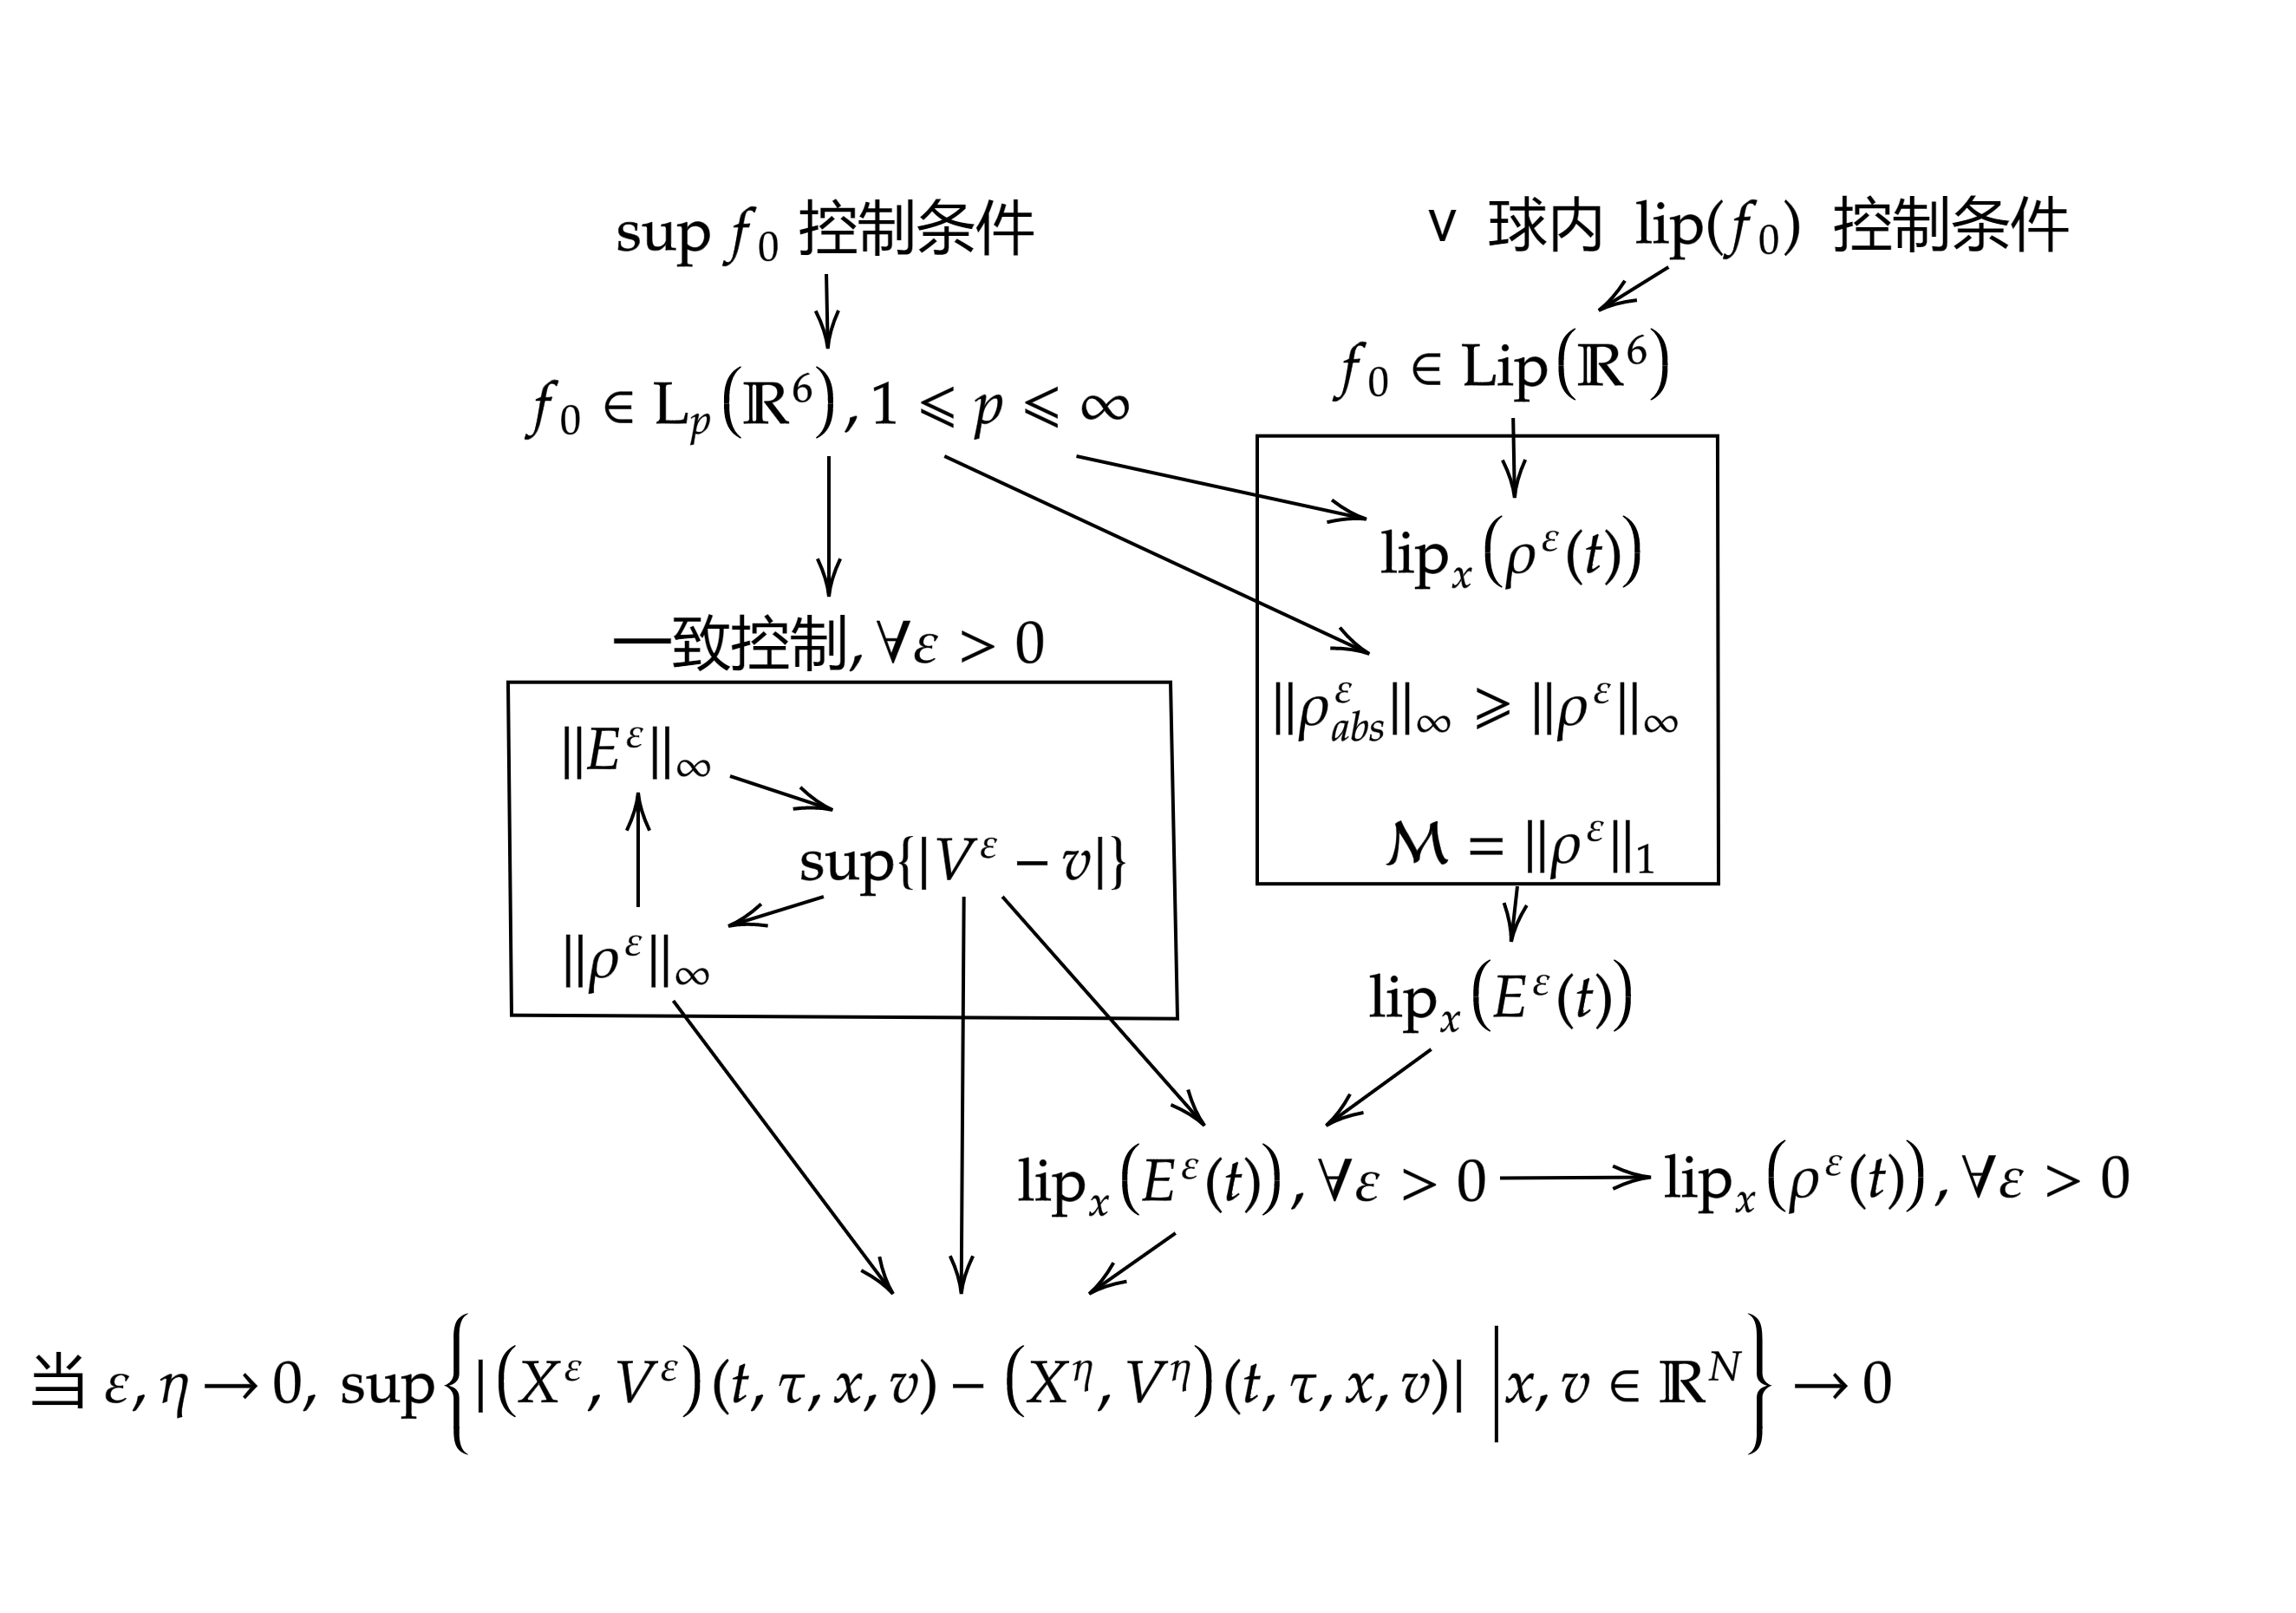
\includegraphics[width=1.0\textwidth]{diagram.png}
    \caption{图中所示为证明适定性过程中各个命题证明的前后序列,其中箭头表示我们证明命题的前后关系,而不是逻辑上的充分关系;出现在图中的变量表示存在 $H\in C_+(I)$ 中函数对其控制,$\forall \varepsilon>0$ 表示对 $\varepsilon$ 一致控制。}
    \label{fig:diagram}
  \end{figure}
  
由于 $\text{VP}^\varepsilon (\varepsilon >0)$ 问题中场函数的奇异性被移除了,经典的分析手段可以很好地处理 $\text{VP}^\varepsilon (\varepsilon >0)$ 的解。要在其基础上,证明 $\text{VP}^0$ 解的存在性和唯一性,我们需要说明 $f^\varepsilon$ 确实在 $I\times \bbR^N \times \bbR^N $ 上当取极限 $\varepsilon\rightarrow 0 $ 时一致收敛到 $f^0$。而 Vlasov 问题中的经典解通常指的是特征线常微分问题有唯一解,我们逐渐往这个方向推进。在图中即为最关键的最后 Cauchy 准则给出的收敛依据,特征线确实随着 $\varepsilon\rightarrow 0$ 收敛,这是在本章最后的第四节完成的。

在此之前我们需要做一些准备工作,如图左侧对区间提出的区间\boundcondition,这部分在下面第二节。我们发现对三者 $\|\vE^\varepsilon(t)\|_\infty$, $\|\rho^\varepsilon(t)\|_\infty$ 和 $\sup \{|\vect{V}^\varepsilon(r,0,\vx,\vv)-\vv| \bigg|\vx,\vv \in \bbR^N, 0\leqslant r \leqslant t \}=:h_v^\varepsilon(t)$ 的一致控制条件是等价的。通过 Gronwall 引理我们找到一定能够控制 $h_v^\varepsilon,\forall \varepsilon>0$ 的函数,从而确定了一定有一段非空区间满足\boundcondition。

然后则是第三节对 $\vE^\varepsilon$ Lipschitz 连续性的一致控制,证明这点需要对密度 $\rho^\varepsilon$ 的 $\mathrm{L}^1$ 和 $\mathrm{L}^\infty$ 范数及其的 Lipschitz 连续性。这里我们需要另外的\lipOffVsphere 来补充需要的初值的 Lipschitz 连续性。

以 $\|\rho^\varepsilon\|_\infty$, $h_v^\varepsilon(t)$ 及 $\operatorname{lip}_x (\vE^\varepsilon(t))$ 三者的一致控制为基础,我们得以证明区间有界条件与局部解存在互为充要条件,从而刻画 Vlasov-Poisson 方程的适定性。

% \section{控制 \texorpdfstring{$\vE^\varepsilon$}{Lg} 和 \texorpdfstring{$\rho^\varepsilon$}{Lg} 及其 Lipschitz 常数}
\section{区间的有界条件}
% \subsection{\texorpdfstring{$\vE^\varepsilon$}{Lg} 和 \texorpdfstring{$\rho^\varepsilon$}{Lg} 有界}
\begin{assumption}
    假设 $f^{\varepsilon}$ 是 $\text{VP}^{\varepsilon}$ $(\varepsilon \geqslant 0 \text{ 定值})$ 问题在 $I$ 上的解
    % Assume that $f^{\varepsilon}$ is a solution of $\text{VP}^{\varepsilon}(\varepsilon \geqslant 0$ fixed) on I. 
    
    \begin{enumerate}
        \item 定义 \underline{ $f_0$ 满足 \supremumf}:如果存在合适的 $K_{1}, K_{2}$ (可以依赖于初值的常数)使得下式对所有的 $a \geqslant 0$ 成立,
        % We say that $f_0$ satisfies \underline{\supremumf}, if
        \begin{equation}
            \label{eq:supremum-f0-control}
            \int^*  \underbrace{\sup \left\{|f_0(\vx,\vect{u})| |\vx,\vect{u} \in \bbR^{N}, | \vect{u} - \vv | \leqslant a\right\} }_{\text{该部分为 } \vv \text{ 的函数}} \mathrm{d} \vv \leqslant K_{1} \cdot\left(K_{2}+a\right)^{N}
        \end{equation}
        ($\int^*  \ldots \mathrm{d} \vx$ 标记为上 Lebesgue 积分)
        % for suitable constants $K_{1}, K_{2}$ and all $a \geqslant 0$ ($\int^*  \ldots \mathrm{d} x_{0}^{N}$ denotes the upper Lebesgue integral)
        
        \item 定义 $f_{0}$ 满足 \underline{\lipOffVsphere} 为:存在一个函数  $h \in C_{+}([0, \infty))$ 使得对所有 $a \geqslant 0$ 有下式,
        % We say that $f_{0}$ satisfies \underline{\lipOffVsphere} if there exists an $h \in C_{+}([0, \infty))$ such that for all $a \geqslant 0$

        \begin{equation}
            \begin{aligned}
                \label{eq:lip_Of_f0_in_vsphere_control}
                \int^* \sup \{
                    \frac{|f_{0}(\vect{y}, \vect{u})-f_{0}(\vect{z}, \vect{w})|}{| (\vect{y}, \vect{u})-(\vect{z}, \vect{w})|}  \bigg| (\vect{y},\vect{u}), (\vect{z},\vect{w}) \in \bbR^{N}\times \bbR^{N},\\ (\vect{y},\vect{u}) \neq (\vect{z},\vect{w}),             \left|\vect{u}-\vv\right|,\left|\vect{w}-\vv\right| \leqslant a\} \mathrm{d} \vv \leqslant h(a)
            \end{aligned}
        \end{equation}
    \end{enumerate} 
\end{assumption}

注意本来这里 $h\in C_+([0,\infty))$ 应该用简介中介绍的符号 $H$,但为与原文吻合用了 $h$。

\textit{注意 } \supremumf 可推导出 $f_0$ 是有界的, 即 $f_0 \in \mathrm{L}_{\infty}\left(\mathrm{R}^{2 N}\right)$。若以 $K_1, K_2$ 满足 \supremumf 的 $f_0$,设 $\hat{f}_0 (\vv)=\sup \left\{|f_0(\vx,\vect{v})| |\vx \in \bbR^{N}\right\}$,若其在 $B_R(\vy)\subset \bbR_{v}^3 $($B_R(\vy)$ 半径为 $R$, 中心为 $\vy\in \bbR^3$ 的开球)中无界,则对于任意的 $C_0>0$ 均可找到 $\hat{f}_0(\vv)>C_0, \vv \in B_R(\vy)$,设 $a=2R$,则\supremumf 判别式左侧积分大于 $CR^N C_0$,而右侧的是固定的 $K_{1} \cdot\left(K_{2}+a\right)^{N}$, 取足够大的 $C_0$ 使不等式不成立引出矛盾。又因为 $f_0 \in \mathrm{L}_{1}\left(\bbR^{2 N}\right)$, 故\supremumf 实际上给出了 $f_0$ 很好的可积性,对任意的 $1 \leqslant p \leqslant \infty$ 有 $f_0 \in \mathrm{L}_{p}\left(\mathrm{R}^{2 N}\right)$。
另外观察 \lipOffVsphere 类似的可导出 $f_{0} \in \operatorname{Lip}\left(\bbR^{2 N}\right)$。
% Remark. It is easily shown that \lipOffVsphere implies $f_{0} \in \operatorname{Lip}\left(\bbR^{2 N}\right)$

% 首先要控制 $\vE^\varepsilon$ 和 $\rho^\varepsilon$;以此为基础,我们还将引出区间满足\boundcondition 的重要概念和等价条件,它是我们得以实现控制的关键。

对 $\vE$ 的积分式粗糙地取积分内各项绝对值则有不等式,即 $\left|E^{\varepsilon}\left(t, \vx \right)\right| \leqslant \int\left|\vx-\vy\right|^{1-N} \cdot\left|\rho^{\varepsilon}_{abs}\right|\left(t, \vy\right) \mathrm{d} \vy$。借助于这个不等式,通过下面的引理及之后的推论可以证明 $\left\|E^{\varepsilon}(t, \cdot)\right\|_{\infty}$ 有界。
% \section{Bounds for \texorpdfstring{$\vE^\varepsilon$}{Lg} and \texorpdfstring{$\rho^\varepsilon$}{Lg} }
% Traditional analysis works well to solve the problem $\text{VP}^\varepsilon (\varepsilon >0)$ due to the removed singularity of integral kernel. However, we need to illustrate that $f^\varepsilon$ uniformly converges to $f^0$ as $\varepsilon\rightarrow 0 $ on $I\times \bbR^N \times \bbR^N $ and confirm the uniqueness. Therefore we need conditions on $f$ which assure that the characteristcs ordinary equations $\vect{X}(s,t_0, \vx,\vv),\vect{V}(s,t_0, \vx,\vv)$ have a unique solution for given parameter $t_0 \in I, \vx, \vv \in \bbR^N$. In this section we take the first steps into this direction. An obvious estimate yields that $\left|E^{\varepsilon}\left(t, \vx\right)\right| \leqslant \int\left|\vx-\vy\right|^{1-N} \cdot\left|f^{\varepsilon}\right|_{Q}\left(t, \vy\right) \mathrm{d} \vx^{N}$
% Here the time $t$ plays only the role of a parameter, whereas integration is with respect to $\vy .$ 

% Therefore we can use the following lemma to find a bound for $\left\|E^{\varepsilon}(t, \cdot)\right\|_{\infty}$
\begin{lemma}
    \label{lem:sigma-influence}
    假设 $0<\alpha<N, p \in( 1, \infty], q \in[1, \infty)$ $p>N /(N-\alpha)>q $ 且 $\sigma \in \mathrm{L}_{p}\left(\bbR^{N}\right) \cap \mathrm{L}_{q}\left(\bbR^{N}\right) .$ 则对于任意的 $\vect{z} \in \bbR^{N}$ 有
    % Assume $0<\alpha<N, p \in( 1, \infty], q \in[1, \infty)$ $p>N /(N-\alpha)>q .$ Assume further $\sigma \in \mathrm{L}_{p}\left(\bbR^{N}\right) \cap \mathrm{L}_{q}\left(\bbR^{N}\right) .$ Then for all $\vect{z} \in \bbR^{N}$

    \begin{equation}
        \label{eq:rho-E-bound}
        \int|\vect{z}-\vect{w}|^{-\alpha} \cdot|\sigma(\vect{w})| \mathrm{d} \vect{w} \leqslant \bar{C}(N, \alpha, p, q) \cdot\|\sigma\|_{p}^{\lambda} \cdot \|\sigma\|_{q} ^{\mu}
    \end{equation}
其中常数有 $\tilde{C}(N, \alpha, p, q)$,   $\lambda:=(\alpha / N-1+1 / q) /(1 / q-1 / p)$ 及 $\mu:=1-\lambda $. 
% with constants $\tilde{C}(N, \alpha, p, q)$,   $\lambda:=(\alpha / N-1+1 / q) /(1 / q-1 / p)$ and $\mu:=1-\lambda $. 

令 $\tilde{C}_{min}(N, \alpha, p, q)$ 为对任意的 $\sigma \in \mathrm{L}_{p}\left(\bbR^{N}\right) \cap \mathrm{L}_{q}\left(\bbR^{N}\right)$, \eqref{eq:rho-E-bound} 式均成立的常数。 
% Let $\tilde{C}_{min}(N, \alpha, p, q)$ denote the smallest constant such that \eqref{eq:rho-E-bound} remains true for all $\sigma \in \mathrm{L}_{p}\left(\bbR^{N}\right) \cap \mathrm{L}_{q}\left(\bbR^{N}\right)$
\end{lemma}

\begin{proof}
    将 \eqref{eq:rho-E-bound} 的积分域分为球内外的两部分 $R>0$,通过  \Holder 不等式,
    % Fix $R>0$ and divide the integral of \eqref{eq:rho-E-bound} into two parts, one for intergral $I_1$ inside a sphere (radius $R$) while the other $I_2$ outside.
    
% By \Holder's inequality,
$$
I_{1} \leqslant  \| |\vect{z}-\vx|^{-\alpha}\cdot 1_{|\vect{z}-\vx|\leqslant R}\|_{p^{\prime}} \|\sigma\|_{p}
= \left(\frac{\omega_N}{N-\alpha p^\prime}\right)^{1/p^\prime} R^{(N / p^{\prime})-\alpha} \|\sigma\|_{p}
$$
$$
I_{2} \leqslant  \| |\vect{z}-\vx|^{-\alpha}\cdot 1_{|\vect{z}-\vx|> R}\|_{q^{\prime}} \|\sigma\|_{q}
= \left(\frac{-\omega_N}{N-\alpha q^\prime}\right)^{1/q^\prime} R^{(N / q^{\prime})-\alpha} \|\sigma\|_{q}
$$

$p^{\prime}$ 和 $q^{\prime}$ 大小为 $p^{-1}+p^{\prime-1}=q^{-1}+q^{\prime-1}=1$。
% $p^{\prime}$ and $q^{\prime}$ being the numbers with $p^{-1}+p^{\prime-1}=q^{-1}+q^{\prime-1}=1$.

上述两式右侧的加和作为 $R$ 的函数取最小值得到 const. $\|\sigma\|_{p}^{\lambda} \cdot\|\sigma\|_{q}^{\mu} .$ , 即 $\tilde{C}(N,\alpha, p, q)\|\sigma\|_{p}^{\lambda} \cdot\|\sigma\|_{q}^{\mu}  $.
% Thus $I_{1}+I_{2} \leqslant$ const. $\left(R^{\left(N / p^{\prime}\right)-\alpha} \cdot\|\sigma\|_{p}+R^{\left(N / q^{\prime}\right)-\alpha} \cdot\|\sigma\|_{q}\right)$
% The minimum of the right-hand side as a function of $R$ is equal to const. $\|\sigma\|_{p}^{\lambda} \cdot\|\sigma\|_{q}^{\mu} .$ , \textit{i.e.} $\tilde{C}(N,\alpha, p, q)\|\sigma\|_{p}^{\lambda} \cdot\|\sigma\|_{q}^{\mu}  $.
\end{proof}

这条引理启发我们研究 $\left\| \rho^{\varepsilon}(t, \cdot)\right\|_{p}$,   $\left\|f^{\varepsilon}(t, \cdot)\right\|_{1}=\mathcal{M}.$ 下面我们还将讨论其 $\mathrm{L}^{\infty}$ 范数,


% This lemma shows us that it makes sense to investigate the properties of $\left\|f^{\varepsilon} \rho_{\theta}(t, \cdot)\right\|_{p} .$ We already know that always $\left\|f^{\varepsilon}(t, \cdot)\right\|_{1}=m .$ Now we consider the case $p=\infty, 1<p<\infty$ will become important in part II.




%  定义\underline{ $f^{\varepsilon}$ 在 $I$ 上满足 \rhoabs }:存在一个函数 $H_{\rho,abs}^{\varepsilon}(t) \in C_{+}(I)$ 使得对所有的 $t \in I$ 有下式,
% We say that $f^{\varepsilon}$ satisfies \underline{\rhoabs on $I$}, if there exists an $C_{\rho,abs}^{\varepsilon}(t) \in C_{+}(I)$ such that for all $t \in I$
% \begin{equation}
%     \label{eq:rhoabs-control}
%     \|\rho^{\varepsilon}_{abs}(t, \cdot)\|_{\infty} \leqslant H_{\rho,abs}^{\varepsilon}(t)
% \end{equation}

% \supremumf demonstrates that $f_0$ is bounded, \textit{i.e.} $f_0 \in \mathrm{L}_{\infty}\left(\mathrm{R}^{2 N}\right)$. As $f_0 \in \mathrm{L}_{1}\left(\bbR^{2 N}\right)$, 
% \supremumf indeed shows strong control on $f_0$ that $f_0 \in \mathrm{L}_{p}\left(\mathrm{R}^{2 N}\right)$ for all $1 \leqslant p \leqslant \infty$.




% \begin{lemma}
%     如果存在常数 $\alpha>N$ 和 $K \geqslant 0$ 使得对任意的 $\vx,\vv \in \bbR^{ N}$ $f_0$ 有 $|f_0(\vx,\vv)| \leqslant K \cdot\left(1+\left|\vv\right|\right)^{-\alpha}$,则 $f_0$ 满足 \supremumf。
%     %  $f_0$ satisfies \supremumf, if there exists constants $\alpha>N$ and $K \geqslant 0$ such that $|f_0(\vx,\vv)| \leqslant K \cdot\left(1+\left|\vv\right|\right)^{-\alpha}$ for all $\vx,\vv \in \bbR^{ N}$
% \end{lemma}

% \begin{proof} 当 $N=1$ 时,可以通过 $K\cdot (1+|\vv|)^{-\alpha}$ 本身满足 \supremumf 来揭示。而对于 $N>1$ 的情形,可以先将 $|\vv|$ 在不等式中拆解成它的分量,
% % This is easily verified when $N=1$ by showing that the $K\cdot (1+|\vv|)^{-\alpha}$ satisfies \supremumf. While for the $N>1$ cases, establish the relation between $|\vv|$ and its components first,
% $
% \left(1+\left| \vv \right|\right)^{-\alpha} \leqslant\left(1+\left|v_1\right|\right)^{-\alpha / N} \cdots \cdot\left(1+\left|v_{N}\right|\right)^{-\alpha / N}
% $
% 并注意,
% % and note that
% \[
% \begin{array}{l}
% \sup \left\{|f_0(\vx, \vect{u})|\left| \vx, \vect{u} \in \bbR^{2 N},\right| \vect{u}-\vv | \leqslant a\right\} \\
% \leqslant K \cdot \sup \left\{\left(1+\left|u_{1}\right|\right)^{-\alpha / N}\bigg| | u_{1}-v_{1} | \leqslant a\right\} 
% \cdot\cdots\cdot \sup \left\{\left(1+\left|u_{N}\right|\right)^{-\alpha / N}\bigg| | u_{N}-v_{N} | \leqslant a \right\}
% \end{array}
% \]

% 等式两侧都对 $\vv$ 空间做上 Lebesgue 积分,而右侧是可测的,其值我们可以通过  Fubini 定理得到。 
% \end{proof}
% Do upper Lebesgue integral in $v$ on both sides and note the right-hand side is measurable and its integral could be acquired using Fubini's theorem. 


% \begin{lemma}
%     \label{lem:sup-f-control}
%     假设 $f^{\varepsilon}$ 是 $\text{VP}^{\varepsilon}$ $(\varepsilon \geqslant 0 \text{ 固定})$ 问题在 $I$ 上的解,并且初值条件 $f_0$ 满足 \supremumf  (记该条件中两常数为 $K_{1}$ 和 $K_{2}$ )。 那么
%     % Assume that $f^{\varepsilon}$ is a solution of $\text{VP}^{\varepsilon}(\varepsilon \geqslant 0$ fixed) on I. Assume further that $f$ satisfies \supremumf (with constants $K_{1}$ and $K_{2}$ ). Then
%  \begin{enumerate}[(i)]
%     \item $f^{\varepsilon}$ 在 $I$ 上满足 \rhoabs.
%     % \item $f^{\varepsilon}$ satisfies \rhoabs on $I$.
%     \item 取任意的 $t_{0} \in I$, 函数 $f^{\varepsilon}\left(t_{0}, \cdot\right)$ 亦满足 \supremumf ,即\supremumf 是可延续的。若 $f^{\varepsilon}$ 满足条件时的常数为 $K_{1}$ 和 $K_{2}$,则 $f^{\varepsilon}\left(t_{0}, \cdot\right)$ 以常数 $K_{1}$ 和 $K_{2}+h_{v}^{\varepsilon}\left(t_{0}\right)$ 满足该条件。
%     % \item For each fixed $t_{0} \in I$ the function $f^{\varepsilon}\left(t_{0}, \cdot\right)$ also satisfies \supremumf with the same constants $K_{1}$ and $K_{2}+h_{v}^{\varepsilon}\left(t_{0}\right)$
%  \end{enumerate}
% \end{lemma}

\begin{proof}
    \begin{enumerate}[(i)]
        \item 对给定的 $t_0\in I$,
        $$\begin{aligned}
            &\sup \left\{\left|f^{\varepsilon}\left(t_{0}, \vy, \vect{u}\right)\right|\left|\vy, \vect{u} \in \mathbb{R}^{2 N},\right| \vect{u}-\vv | \leqslant a\right\}\\
        =&\sup \left\{\left|f_0\left(  \vect{X}^{\varepsilon}\left(0, t_{0}, \vy, \vect{u}\right), \vect{V}^{\varepsilon}\left(0, t_{0}, \vy, \vect{u}\right) \right) \right|  \bigg| \vy,\vect{u} \in \mathbb{R}^{ N},\left|\vect{u}-\vv\right| \leqslant a\right\}\\
        \leqslant &\sup \left\{|f_0(\vy, \vect{u})|\left|\vy,\vect{u} \in \mathrm{R}^{N},\right| \vect{u}-\vv | \leqslant a+h_{v}^{\varepsilon}\left(t_{0}\right)\right\}
        \end{aligned}$$
        
        于是对其积分中可知 $f(t_0, \cdot, \cdot)$ 也满足 \supremumf,只是常数的大小发生了改变。
        % It follows that an integral would suffice to show that $f(t_0, \cdot, \cdot)$ satisfy the \supremumf.
    \end{enumerate}
\end{proof}

% \begin{lemma}
    
% 假设 $f^{\varepsilon}$ 是 $\text{VP}^{\varepsilon}(\varepsilon \geqslant 0) $ 在 $I$ 上的解且假设 $f_0$ 在 $\bbR^{2 N}$ 上连续并满足 \supremumf。则 $f^{\varepsilon}$ 在 $I \times \bbR^{2N}$ 上是连续的。
% \end{lemma}

% (2.6) Lemma Assume that $f^{\varepsilon}$ is a solution of $\text{VP}^{\varepsilon}(\varepsilon \geqslant 0 \text { fixed) on } I$. Assume further that $f$ is continuous on $\bbR^{2 N}$ and satisfies $(f 1) .$ Then $f^{\varepsilon}$ is continuous on $I \times \bbR^{N}$

\begin{theorem}\textit{(有界条件的等价性)}
    \label{eq:bound-equivalent}
    假设 $I \subset[0, \infty)$ 是个包含 $0 $ 的区间,并且 $f_{0}$ 满足 \supremumf 的条件,那么下面三个条件是等价的:
    

    \begin{enumerate}[(i)]
        \item 存在函数 $H_{\rho}(t) \in C_{+}(I)$, 使得
         $$\left|\rho^{\varepsilon}\left(t, \vx\right)\right| \leqslant H_{\rho}(t) \text{ 对任意的 } \varepsilon>0, t \in I, \vx \in \bbR^{\mathrm{N}}$$
        \item 存在函数 $H_{E}(t) \in C_{+}(I)$, 使得
        $$\left|\vE^{\varepsilon}\left(t, \vx\right)\right| \leqslant H_{E}(t) \text{ 对任意的 } \varepsilon>0, t \in I, \vx \in \bbR^{\mathrm{N}}$$
        \item 存在函数 $H_{v}(t) \in C_{+}(I)$, 使得
        $$ | \vect{V}^{\varepsilon}(t, 0, \vx, \vv)-\vv | \leqslant h_{v}^{\varepsilon}(t) \leqslant H_{v}(t) \text{ 对任意的 } \varepsilon>0, t \in I, \vx,\vv \in \bbR^{N}$$
    \end{enumerate}
\end{theorem}

\begin{definition}\textit{(有界条件)}
    \label{de:boundness}
    如果以上的这些条件能够被满足,定义 $I$ 满足“有界条件”。
    % 如果 $N=1,2,$ 那么 $[0, \infty) $ 都满足该条件。 而对于 $ N \geqslant 3$ 的情况,存在一个区间 $T \in( 0, \infty]$,右端点依赖于空间维度 $N, \mathcal{M}:=\|f_{0}\|_{1}$ 和 $K_{1}, K_{2}$ (\supremumf 中约定的常数), 使得 $[0, T)$ 满足有界条件。
    
    % 也就是说,一个区间是不是满足“有界条件”,并不完全取决这个区间本身,还和 $\text{VP}^\varepsilon$ 给定的问题维度及初值按多项式衰减的不等式的系数有关。
\end{definition}

\begin{proof}
    证明他们互相充要的工具其实我们已经准备好了。

    (i) $\Rightarrow$(ii)  由引理 (2.1)$(\alpha=N-1, p=\infty, q=1)$ \\
    $\left|\vE^{\varepsilon}\left(t, \vx\right)\right| \leqslant \tilde{C}_{min}(N, N-1, \infty, 1) \cdot\left(\left\|\rho^{\varepsilon}(t, \cdot)\right\|_{\infty}\right)^{(N-1) / N} \cdot \mathcal{M}^{1 / N}.$

    % 下面两个推导,都出现在了引理 \ref{lem:sup-f-control} 中,

        (ii) $\Rightarrow$ ( iii) : $ h_{v}^{\varepsilon}(t) \leqslant \int_{0}^{t} \sup \left\{\left\|E^{\varepsilon}(\tau, \cdot)\right\|_{\infty} | 0 \leqslant \tau \leqslant r\right\} \mathrm{d} r$

        (iii) $\Rightarrow$ (i):  对任意的 $t \in I$,令 
        % For all $t \in I$, let 
        \[
        \begin{array}{l}
        \begin{aligned}
        h_{v}^{\varepsilon}(t): &=\sup \left\{\left|\vect{V}^{\varepsilon}(0, \tau, \vx, \vv)-\vv\right| \bigg| \vx,\vv \in \bbR^{N}, 0 \leqslant \tau \leqslant t\right\} \\
        &=\sup \left\{\left|\vect{V}^{\varepsilon}(\tau, 0, \vx, \vv)-\vv\right| \bigg| \vx,\vv \in \mathbb{R}^{N}, 0 \leqslant \tau \leqslant t\right\} \\
        &\text{\small 速度最大改变量应被场强上确界控制住}\\
        % &\text{\small The maximum possible velocity change should be controlled by the supreme field intensity.}\\
        & \leqslant \int_{0}^{t} \sup \left\{\| \vE^{\varepsilon}(\tau, \cdot) \|_\infty \bigg| 0 \leqslant \tau \leqslant r\right\} \mathrm{d} r =: \int_{0}^{t} h_{E}^{\varepsilon}(r) \mathrm{d} r<\infty 
        \end{aligned}
        \end{array}
        \]
        于是,因为速度的最大改变量被 $h_v^\varepsilon(t)$ 控制住了,只有那些速度相近的“粒子“对于任意的才能在 $t$ 时刻到达 $\vx,\vv \in \mathbb{R}^{ N}$。
        
        % It follows that only the particles with a 'neighboring' velocity can arrive at $(\vx, \vv)$ at time $t$, because the maximal change of velocity is  controlled by the $C_v^\varepsilon(t)$, for all $x \in \mathrm{R}^{2 N}$
        \[
        \begin{aligned}
        \left|f^{\varepsilon}(t, \vx, \vv)\right| &=\left|f_0\left(\vect{X}^{\varepsilon}(0, t, \vx, \vv), \vect{V}^{\varepsilon}(0, t, \vx, \vv)\right)\right| \\
        & \leqslant \sup \left\{|f_0(\vect{y}, \vect{u})|\left|\vect{y},\vect{u} \in \mathbb{R}^{N},\right| \vect{u}-\vect{v} | \leqslant h_{v}^{\varepsilon}(t)\right\}
        \end{aligned}
        \]
        左侧 $\int \ldots d \vv$ 积分,右侧 $\int_{\cdots}^{*} \ldots d \vv$ 上 Lebesgue 积分可得 $\rho^{\varepsilon}_{abs}\left(t, \vx\right) \leqslant K_{1} \cdot\left(K_{2}+h_{v}^{\varepsilon}(t)\right)^{N}$.
        % Taking $\int \ldots d \vv$ of the left-hand side and $\int_{\cdots}^{*} \ldots d \vv$ of the right-hand side proves $\rho^{\varepsilon}_{abs}\left(t, \vx\right) \leqslant K_{1} \cdot\left(K_{2}+h_{v}^{\varepsilon}(t)\right)^{N}$.
        
        $\left| \rho^{\varepsilon} \left(t, \vx \right)\right| \leqslant K_{1} \cdot\left(K_{2}+h_{v}^{\varepsilon}(t)\right)^{N}\leqslant K_{1} \cdot\left(K_{2}+h_{v}(t)\right)^{N}$

相互等价关系得证。
\end{proof}

% \begin{theorem}\textit{(Boundness Conditions Equivalence)}

%     Assume  $I \subset[0, \infty)$ is an interval with $0 \in I $. Assume  further that $f_{0}$ satisfies $(f_{0} 1)$
%     Then the following statements are equivalent:

%     \begin{enumerate}[(i)]
%         \item There exists an $H_{\rho}(t) \in C_{+}(I),$ such that 
%          $$\left|\rho^{\varepsilon}\left(t, \vx\right)\right| \leqslant H_{\rho}(t) \text{ for all } \varepsilon>0, t \in I, \vx \in \bbR^{\mathrm{N}}$$
%         \item There exists an $H_{E}(t) \in C_{+}(I),$ such that 
%         $$\left|\vE^{\varepsilon}\left(t, \vx\right)\right| \leqslant H_{E}(t) \text{ for all } \varepsilon>0, t \in I, \vx \in \bbR^{\mathrm{N}}$$
%         \item There exists an $H_{v}(t) \in C_{+}(I),$ such that 
%         $$ | \vect{V}^{\varepsilon}(t, 0, \vx, \vv)-\vv | \leqslant C_{v}^{\varepsilon}(t) \leqslant h_{v}(t) \text{ for all } \varepsilon>0, t \in I, \vx,\vv \in \bbR^{N}$$
%     \end{enumerate}
% \end{theorem}


现我们仅依靠定理 \ref{thm:epsilon-greater-0} 的解的存在性,希望给出一个上面条件需要的控制函数。对于一个固定的 $\varepsilon$,令 $h_{v+}^\varepsilon:=K_2+h_v^\varepsilon(t)$,上面三式联立可得下式成立,

\begin{equation}
h_{v+}^\varepsilon(t) \leqslant K_{2}+\int_{0}^{t} K_{3} \cdot(h_{v+}^\varepsilon(r))^{N-1} \mathrm{d} r \\
\end{equation}
其中,$K_{3}:=\tilde{C}_{min}(N, N-1, \infty, 1) \cdot \mathcal{M}^{1 / N} \cdot\left(K_{1}\right)^{(N-1) / N}$。发现它确实是非线性 Gronwall 引理 \ref{lem:nonlinear-Gronwall} 所适用的不等式,从而我们对 $h_{v+}^\varepsilon(t) $ 的大小可以控制住,被该不等式容许的最大的解 $g$,即常微分方程 $g^{\prime}=K_{3} \cdot(g)^{N-1}, g(0)=K_{2}$ 的解所控制。当 $N\neq 2$ 时,$g(t) = [(-N+2)K_3 t+K_2^{-N+2}]^{\frac{1}{-N+2}}$。它能够在一段区间 $[0, K_2^{-(N-2)}/(N-2)K_3)$ 内控制住 $h_{v}^\varepsilon(t) \leqslant h_{v+}^\varepsilon(t) \leqslant g(t)$。  $N=1,2$ 时易见可以全局控制,则满足有界条件的 $I=[0, \infty)$。$N \geqslant 3$ 的情况只能根据 $K_1,K_2,\mathcal{M}$ 及空间维度 $N$ 给出一个满足有界条件的非空区间, $I=[0, T), T \in( 0, \infty]$.


% \begin{definition}\textit{(Boundness Condition)}

%     If the above conditions are satisfied, we say that "$I$ satisfies the boundedness condition"
%     If $N=1,2,$ then $[0, \infty) $ satisfies the boundedness condition.
%     $\text {If }N \geqslant 3$, there exists a $T \in( 0, \infty],$ which depends only on $N, \mathcal{M}=\|f_{0}\|_{1}$ and $K_{1}, K_{2}$ (the constants from definition (2.3)), such that $[0, T)$ satisfies the  boundedness condition.
    
% \end{definition}



\section{\texorpdfstring{$\vE^{\varepsilon}$}{Lg} 的 Lipschitz 连续性}
% \subsection{\texorpdfstring{$\vE^{\varepsilon}$ 和 $\rho^{\varepsilon}$}{Lg} 的 Lipschitz 连续性}
% \section{\texorpdfstring{$\vE^{\varepsilon}$ 和 $\rho^{\varepsilon}$}{Lg} 的 Lipschitz 连续性}
% \section{Lipschitz Continuity of \texorpdfstring{$\vE^{\varepsilon}$ and $\rho^{\varepsilon}$}{Lg}}

本节将证明如果 $f_{0}$ 足够得好, $\vE^{\varepsilon}(t, \cdot)$ 和 $\rho^{\varepsilon}(t, \cdot)$ 便是 Lipschitz 连续的。当 $I$ 满足有界条件时,其 Lipschitz 常数不依赖于 $\varepsilon$。

在下面的引理中,我们实际上在尝试通过用 $\rho^\varepsilon$ 的范数及 Lipschitz 常数来控制 $\operatorname{lip}_x (\vE^\varepsilon)$。%我们先给定 $\sigma$ 一个较大的函数空间,然后说明能通过它来控制住它产生的场 $lip(\vE^\varepsilon)$ 的 Lipschitz 常数,进而由于 $\rho^\varepsilon$ 确实在该空间中,$\text{VP}^\varepsilon$ 问题的解对应产生的场的强度 $\vE$ 应该对任意的 $t\in I$ 都是 Lipschitz 连续的。
% In this section we show that $\vE^{\varepsilon}(t, \cdot)$ and $\rho^{\varepsilon}(t, \cdot)$ are Lipschitz continuous, if $f_{0}$ is sufficiently nice. If $I$ satisfies the boundedness condition, the Lipschitz constants do not depend on $\varepsilon$

\begin{lemma}
    \label{lem:lip-E}
    令 $\varepsilon \geqslant 0, \gamma=\pm 1$。假设 $\sigma: I \times \bbR^{N} \rightarrow \bbR$ 对任意的 $t \in I$ 满足 $\sigma(t, \cdot) \in \mathrm{L}_{1}\left(\bbR^{N}\right) \cap \mathrm{L}_{\infty}\left(\bbR^{N}\right) \cap \operatorname{Lip}\left(\bbR^{N}\right)$ 。 令  $\vE^\varepsilon\left(t, \vx\right):=\int \vect{e}^{\varepsilon}\left(\vx-\vect{y}\right) \cdot \sigma\left(t, \vect{y}\right) \mathrm{d} \vect{y}, t \in I, \vx,\vect{y} \in \bbR^{N} .$ 则有
    % Let $\varepsilon \geqslant 0, \gamma=\pm 1$. Assume that $\sigma: I \times \bbR^{N} \rightarrow \bbR$ satisfies $\sigma(t, \cdot) \in \mathrm{L}_{1}\left(\bbR^{N}\right) \cap \mathrm{L}_{\infty}\left(\bbR^{N}\right) \cap \operatorname{Lip}\left(\bbR^{N}\right)$ for all $t \in I$. Let  $\vE^\varepsilon\left(t, \vx\right):=\int \vect{e}^{\varepsilon}\left(\vx-\vect{y}\right) \cdot \sigma\left(t, \vect{y}\right) \mathrm{d} \vect{y}, t \in I, \vx,\vect{y} \in \bbR^{N} .$ Then
\begin{enumerate}[(i)]
    \item 对任意的 $t \in I$ 有 $\vE^\varepsilon(t, \cdot) \in C_{b}^{1}\left(\bbR^{N}, \bbR^{N}\right)$ 和下式

    \[
    \begin{aligned}
        \left|\frac{\partial E_{i}}{\partial x_{j}}\left(t, \vx\right)\right| \leqslant &\omega_{N} ( \delta_{i j}/N+N) + N \omega_N \ln (1+\operatorname{lip}(\sigma(t, \cdot))) \|\sigma(t, \cdot)\|_{\infty} \\
          &+ N\|\sigma(t, \cdot)\|_{1} 
    \quad \text { for all } 1 \leqslant i, j \leqslant N, t \in I, \vx=\left(x_{1}, \ldots, x_{N}\right) \in \bbR^{N}
    \end{aligned}
    \]
    于是 $\vE^\varepsilon(t, \cdot) \in \operatorname{Lip}\left(\bbR^{N}, \bbR^{N}\right)$ 且
    \[
    \begin{aligned}
    \operatorname{lip}(\vE^\varepsilon(t, \cdot)) \leqslant & \omega_{N}\left(N^{-1}+N^{2} \cdot \log (1+\operatorname{lip}(\sigma(t, \cdot)))\right) \cdot\|\sigma(t, \cdot)\|_{\infty} \\
    &+N^{2}\left(\omega_{N}+\|\sigma(t, \cdot)\|_{1}\right)
    \end{aligned}
    \]
    % \item 如果 $\sigma$ 在 $I \times \bbR^{N}$ 上连续且 $\operatorname{lip}(\sigma(t, \cdot))$ 和 $\|\sigma(t, \cdot)\|_{1}$ 在 $I$ 的任何紧子区间上对 $t$ 都一致有界,则偏导数 $\partial E_{i} / \partial x_{j}$ 在 $I \times \bbR^{N}$ 上连续。
    
    % If $\sigma$ is continuous on $I \times \bbR^{N}$ and if $\operatorname{lip}(\sigma(t, \cdot))$ and $\|\sigma(t, \cdot)\|_{1}$ are bounded uniformly in t on every compact subinterval of $I,$ then the partial derivatives
    % $\partial E_{i} / \partial x_{j}$ are continuous on $I \times \bbR^{N}$
    
\end{enumerate}

\end{lemma}

\begin{proof}
    \begin{enumerate}[(i)]
        \item $E_i^\varepsilon(t,\vx)$ 偏导可以被拆分为球壳型的三个部分。令被求点的位置 $\vx$ 位于开球 $B(\vect{z},d_1)$ 内,球心 $\vect{z}$ 和半径 $d_1$. 
        \begin{equation}
            \frac{\partial}{\partial x_j} E_i^\varepsilon(\vx)= \int_{d_1<|\vx-\vy|\leqslant d_2}+\int_{d_2<|\vx-\vy|}+\int_{|\vx-\vy|\leqslant d_1} \frac{\partial}{\partial x_j} e_i^\varepsilon (\vx - \vy) \sigma(t,\vy)\mathrm{d} \vy  =: I_{1,1} + I_{1,2} +I_{2}
        \end{equation}
    
        $\vect{e}^\varepsilon$ 的定义给出 $\Biggl|\frac{\partial}{\partial x_j} e_i^\varepsilon(\vx-\vy) \Biggr|\leqslant N\bigg|\vx-\vy\bigg|^{-N}$ 来帮助控制其中的积分项的估计,参考 \cite*{hellwig1964partial}, 章节 4.4.1, 定理 3 来计算含奇异性的 $I_2$ 积分。 
        % Definition of $\vect{e}^\varepsilon$ gives $\Biggl|\frac{\partial}{\partial x_j} e_i^\varepsilon(\vx-\vy) \Biggr|\leqslant N\bigg|\vx-\vy\bigg|^{-N}$ to control the estimate, and \textit{cf.} [10], section 4.4.1, theorem 3 helps settle the singularity calculation problem of $I_2$. 
        
         由于该不等式部分参数选取 $d_1,d_2$ 较为主观,故证明细节不在这里呈现而请读者查阅原始证明 \cite*{HorstClasssicalI} Sect. 3。
         
        % \item The calculation of $\vE_i^\varepsilon(t,\vx)$ derivative component can be divided into three parts, for which a spherical region decomposition is necessary. Let $\vx$ be in $B(\vect{z},d_1)$, an open sphere with center $\vect{z}$ and radius $d_1$. 
        % \begin{equation}
        %     \frac{\partial}{\partial x_j} E_i^\varepsilon(\vx)= \int_{d_1<|\vx-\vy|\leqslant d_2}+\int_{d_2<|\vx-\vy|}+\int_{|\vx-\vy|\leqslant d_1} \frac{\partial}{\partial x_j} e_i^\varepsilon (\vx - \vy) \sigma(t,\vy)\mathrm{d} \vy  =: I_{1,1} + I_{1,2} +I_{2}
        % \end{equation}
    
        % Definition of $\vect{e}^\varepsilon$ gives $\Biggl|\frac{\partial}{\partial x_j} e_i^\varepsilon(\vx-\vy) \Biggr|\leqslant N\bigg|\vx-\vy\bigg|^{-N}$ to control the estimate, and \textit{cf.} [10], section 4.4.1, theorem 3 helps settle the singularity calculation problem of $I_2$. 
        %  TODO!
        % The details would not be present here because the result in fact is not optimal due to the casual value of $d_1, d_2$.

        % choose $d_1= 1/(1+\operatorname{lip}(\sigma(t,\cdot)))$ and $d_2=1$ then we can deduce that $I_{1,1}+I_{1,2}\leqslant N\omega_N \log{d_2/d_1}\|\sigma(t,\cdot)\|_\infty+ N d_2^{-N}\|\sigma(t,\cdot)\|_1$.
        % \item TODO 
    \end{enumerate}

    
\end{proof}

% 下面我们又提出两个关键假设,其中\lipOffVsphere 能帮助我们很好地控制速度空间的积分,并且它的假设成立并不困难,后面我们将会提出引理使得该假设的达成变得相当简单。



% \begin{lemma}
%     如果 $f_{0}$ 是可导的并存在常数 $\alpha > N$ 和 $K \geqslant 0$ 使得对所有的 $\vx,\vv \in \bbR^{N}$ 有 $\left|\nabla_{x,v}f_{0}(\vx,\vv)\right| \leqslant K \cdot\left(1+\left|\vv\right|\right)^{-\alpha}$ ,便有 $f_{0}$ 满足 \lipOffVsphere。
%     % Assume $f_{0}$ satisfies \lipOffVsphere, if $f_{0}$ is differentiable and there exists constants $\alpha > N$ and $K \geqslant 0$ such that $\left|\nabla_{x,v}f_{0}(\vx,\vv)\right| \leqslant K \cdot\left(1+\left|\vv\right|\right)^{-\alpha}$ for all $\vx,\vv \in \bbR^{N}$
% \end{lemma}

% \begin{proof}
%     通过中值定理,\lipOffVsphere 中的积分式被 $K \cdot\left(\max \left\{1,1+\left|\vv\right|-a\right\}\right)^{-\alpha} $ 控制住了, 令 $ h(a):=K \cdot \omega_{N} \cdot \int_{0}^{\infty} r^{N-1} \cdot(\max \{1,1+r-a\})^{-\alpha} \mathrm{d} r$ 即为所需的 $h(a)$。
%     % By the mean value theorem the integrand of $(3.3 .1)$ is bounded by $K \cdot\left(\max \left\{1,1+\left|\vv\right|-a\right\}\right)^{-\alpha} . \operatorname{Let} h(a):=K \cdot \omega_{N} \cdot \int_{0}^{\infty} r^{N-1} \cdot(\max \{1,1+r-a\})^{-\alpha} \mathrm{d} r$
% \end{proof}

接下来则是本节的关键,要证明 $\vE^\varepsilon$ 和 $\rho^\varepsilon$ 在 $\varepsilon>0$ 时的 Lipschitz 连续性。
\begin{lemma}
    假设 $f_{0}$ 满足 \supremumf 和 \lipOffVsphere 两个条件。
    % Assume that $f_{0}$ satisfies $(f_0 1)$ and \textit{$\operatorname{lip}(f_0)$ in $v$ Sphere Control Condition},

    % 如果 $f^{\varepsilon}$ 是 $\text{VP}^{\varepsilon}$ 在 $I(\varepsilon \geqslant 0 \text { fixed})$ 上的解, 则 $f^{\varepsilon}$ 满足 \lipxOfrho。
        % \item If $f^{\varepsilon}$ is a solution of $\text{VP}^{\varepsilon}$ on $I(\varepsilon \geqslant 0 \text { fixed}),$ then $f^{\varepsilon}$ satisfies \lipOffVsphere.
    如果 $I$ 满足 \boundcondition, 存在函数 $H_{lip(\rho)}, H_{lip(E)} \in C_{+}(I)$ 使得对任意的 $\varepsilon>0, t \in I$ 有
        % \item If $I$ satisfies \boundcondition, there exist functions $C_{\rho}, C_{E} \in C_{+}(I)$ such that for all $\varepsilon>0, t \in I$
        \[
        \operatorname{lip}\left(\vE^{\varepsilon}(t, \cdot)\right) \leqslant H_{lip(E)}(t), \quad \operatorname{lip}\left(\rho^{\varepsilon}(t, \cdot)\right) \leqslant H_{lip(\rho)}(t)
        \]
\end{lemma}

\begin{proof}
    先证存在一个函数 $H_{lip_x(\rho)}^{\varepsilon}(t) \in C_{+}(I)$ 使得对任意的 $t \in I$
% We say that $f^{\varepsilon}$ satisfies \underline{\lipxOfrho on $I$} if there exists a $H_{lip_x(\rho)}^{\varepsilon}(t) \in C_{+}(I)$ such that for $t \in I$
\begin{equation}
    \label{eq:lipx_rho_control}
    \operatorname{lip}\left(\rho^{\varepsilon}(t, \cdot)\right) \leqslant H_{lip_x(\rho)}^{\varepsilon}(t)
\end{equation}

    已在引理 \ref{lem:sup-f-control} 中证明对任意的 $t \in I $ $\sup\left\{\left|\vect{V}^{\varepsilon}(0, \tau, \vx, \vv)-\vv\right|  \bigg|\vx, \vv\in \bbR^{N}\right.,0 \leqslant \tau \leqslant t\}=h_{v}^{\varepsilon}(t)<\infty$。 现对 $\vE$ 的Lipschitz 常数在时间上取上界得到函数 $h^{\varepsilon}_{lip(E)}(t):=\sup \left\{\operatorname{lip}\left(\vE^{\varepsilon}(r, \cdot)\right) | 0 \leqslant r \leqslant t\right\}$
     通过它控制不同特征线在 $\text{VP}^\varepsilon$ 问题解中渐行渐远的尺度, 

     $$
\begin{aligned}
    &\left|(\vect{X}^{\varepsilon}, \vect{V}^{\varepsilon})(t, \tau, \vx, \vv)-(\vect{X}^{\varepsilon}, \vect{V}^{\varepsilon})(t, \tau, \vy, \vect{u})\right| \\
    =&| (\vx,\vv)-(\vy,\vect{u}) |+\int_{\tau}^{t}\left(\vect{V}^{\varepsilon}(r, \tau, \vx, \vv)-\vect{V}^{\varepsilon}(r, \tau, \vy, \vect{u}), \vE^{\varepsilon}\left(r, \vect{X}^{\varepsilon}(r, \tau, \vx, \vv)\right)-\vE^{\varepsilon}\left(r, \vect{X}^{\varepsilon}(r, \tau, \vy, \vect{u})\right)\right) \mathrm{d} r  \\
    \leqslant &| (\vx,\vv)-(\vy,\vect{u}) |+\int_{\tau}^{t}\left(1+h^{\varepsilon}_{lip(E)}(r)\right) \cdot\left|\vect{X}^{\varepsilon}(r, \tau, \vx, \vv)-\vect{X}^{\varepsilon}(r, \tau, \vy, \vect{u})\right| \mathrm{d} r
\end{aligned}
$$
而要用到非线性的 Gronwall 引理 \ref{lem:nonlinear-Gronwall} 则需要连续函数,我们便需要找 $H^{*} \in C_{+}(I)$ 且 $H^{*}(t) \geqslant h^{\varepsilon}_{lip(E)}(t), t \in I $ 的函数暂时替换掉 $h^{\varepsilon}_{lip(E)}(t)$ 运用非线性的 Gronwall 引理有
\[
\text{上式} \leqslant| (\vx,\vv)-(\vy,\vect{u})| \cdot \exp \left(\left|\int_{\tau}^{t}\left(1+H^{*}(r)\right) \mathrm{d} r\right|\right)
\]

\[
\Rightarrow \operatorname{lip}_{x,v}\left((\vect{X}^{\varepsilon},\vect{V}^{\varepsilon})(t, \tau, \cdot)\right) \leqslant \exp \left(\left|\int_{\tau}^{t}\left(1+H^{*}(r)\right) \mathrm{d} r\right|\right)
\]
虽然上面的过程中我们需要额外找 $C_{+}(I)$ 中的函数,但它并不本质,我们总可以在 $C_{+}(I)$ 中找一个单调减的序列,它几乎处处收敛于 $h^{\varepsilon}_{lip(E)}$. 从而上式中的 $H^{*}(t)$ 又可以换回 $h^{\varepsilon}_{lip(E)}(t)$ 

\begin{equation}
    \label{eq:lip-xv-XV}
    \operatorname{lip}_{x,v}\left((\vect{X}^{\varepsilon},\vect{V}^{\varepsilon})(t, \tau, \cdot)\right) \leqslant \exp \left(\left|\int_{\tau}^{t}\left(1+h^{\varepsilon}_{lip(E)}(r)\right) \mathrm{d} r\right|\right)
\end{equation}


有了上面的工具后我们可以正式研究 $\rho^\varepsilon$ 了,令 $\vx, \vy \in \mathbb{R}^{N}$
\[
\begin{array}{l}
\left|\rho^{\varepsilon}\left(t, \vx\right)-\rho^{\varepsilon}\left(t, \vy\right)\right| \leqslant \int\left|f^{\varepsilon}\left(t, \vx, \vv\right)-f^{\varepsilon}\left(t, \vy, \vv\right)\right| \mathrm{d} \vv \\
=\int\left|f_{0}\left((\vect{X}^{\varepsilon},\vect{V}^{\varepsilon})\left(0, t, \vx, \vv\right)\right)-f_{0}\left((\vect{X}^{\varepsilon},\vect{V}^{\varepsilon})\left(0, t, \vy, \vv\right)\right)\right| \mathrm{d} \vv \\
\leqslant \int^* \sup \left\{ \frac{|f_{0}(\vx, \vect{u})-f_{0}(\vy, \vect{w})|}{|(\vx, \vect{u})-(\vy, \vect{w})|} \bigg|(\vx,\vect{u}) \neq (\vy,\vect{w}),| \vect{u}-\vv|,| \vect{w}-\vv | \leqslant h_{v}^{\varepsilon}(t)\right\} \\
\quad \cdot\left|(\vect{X}^{\varepsilon},\vect{V}^{\varepsilon})\left(0, t, \vx, \vv\right)-(\vect{X}^{\varepsilon},\vect{V}^{\varepsilon})\left(0, t, \vy, \vv\right)\right| \mathrm{d} \vv \\
\leqslant h\left(h_{v}^{\varepsilon}(t)\right) \cdot\operatorname{lip}_{x,v}\left((\vect{X}^{\varepsilon},\vect{V}^{\varepsilon})(0, t, \cdot)\right) \cdot\left|\vx-\vy\right|
\end{array}
\]
$h$ 是\lipOffVsphere 中给定的控制函数,于是
\[
\begin{aligned}
\operatorname{lip}\left(\rho^{\varepsilon}(t, \cdot)\right) & \leqslant h\left(h_{v}^{\varepsilon}(t)\right) \cdot \operatorname{lip}_{x,v}\left((\vect{X}^{\varepsilon},\vect{V}^{\varepsilon})(0, t, \cdot)\right)  \\
& \leqslant h\left(h_{v}^{\varepsilon}(t)\right) \cdot \exp \left(\int_{0}^{t}\left(1+h^{\varepsilon}_{lip(E)}(r)\right) \mathrm{d} r\right)
\end{aligned}
\]


如果 $I$ 满足\boundcondition , 我们之前的有界等价条件定理中曾经提到存在 $h_v \in C_{+}(I)$ 使得对任意的 $\varepsilon>0, t \in I$ 有 $h_{v}^{\varepsilon}(t) \leqslant h_{v}(t) $ 说明对 $\varepsilon$ 是一致有界的,于是

\begin{equation}
    \label{eq:lip-rho-control}
    \operatorname{lip}\left(\rho^{\varepsilon}(t, \cdot)\right) \leqslant h\left(h_{v}(t)\right) \cdot \exp \left(\int_{0}^{t}\left(1+h^{\varepsilon}_{lip(E)}(r)\right) \mathrm{d} r\right)
\end{equation}

\boundcondition 还告诉我们存在 $H_{\rho} \in C_{+}(I),$ 使得对所有的  $\varepsilon>0, t \in I$ 有
\begin{equation}
    \|\rho^{\varepsilon}(t, \cdot)\|_{\infty} \leqslant H_{\rho}(t)
\end{equation}

通过上述两式可以将引理 \ref{lem:lip-E} 中一些对 $\varepsilon$ 依赖的项替换掉,可导出对任意的 $t \in I$,有
\[
\begin{aligned}
\operatorname{lip}\left(E^{\varepsilon}(t, \cdot)\right) \leqslant & \omega_{N}\left(N^{-1}+N^{2} \cdot \log \left(1+\operatorname{lip}\left(\Phi_{Q}^{\varepsilon}(t, \cdot)\right)\right)\right) \cdot H_{\rho}^{\varepsilon}(t) +N^{2} \cdot\left(\omega_{N}+\mathcal{M}\right) \\
\leqslant & \omega_{N} \cdot\left(N^{-1}+N^{2} \cdot \log \left(1+h\left(h_{v}(t)\right)\right.\right.\\
&\left.\left.\cdot \exp \left(\int_{0}^{t}\left(1+h^{\varepsilon}_{lip(E)}(r)\right) \mathrm{d} r\right)\right)\right) \cdot H_{\rho}(t)+N^{2} \cdot\left(\omega_{N}+\mathcal{M}\right) \\
=& \omega_{N} \cdot\left(N^{-1}+N^{2} \cdot\left(\log \left(1+h\left(h_{v}(t)\right)\right)\right.\right.\\
&\left.\left.+\int_{0}^{t}\left(1+h^{\varepsilon}_{lip(E)}(r)\right) \mathrm{d} r\right)\right) \cdot H_{\rho}(t)+N^{2} \cdot\left(\omega_{N}+\mathcal{M}\right)
\end{aligned}
\]
右式是对 $t$ 单调增的,所以我们把左式对 $t$ 求上界也没有问题,不等式仍然成立,即不等式左侧变换为 $\sup \left\{\operatorname{lip}\left(E^{\varepsilon}(r, \cdot)\right) | 0 \leqslant r \leqslant t\right\}=h^{\varepsilon}_{lip(E)}(t) .$ 注意这时候我们又可以用非线性的 Gronwall 引理了 \ref{lem:nonlinear-Gronwall}。虽然这个不等式很长,但是 Gronwall 定理告诉我们, $h^{\varepsilon}_{lip(E)}$ 有对应的不依赖于 $\varepsilon$ 的积分式 $H_{lip(E)}$ 控制住它。 

回到本小节证明的开头的不等式 \ref{eq:lip-rho-control},现在等号右边的 $h^{\varepsilon}_{lip(E)}$ 对 $\varepsilon$ 依赖可以去掉了
\[
\operatorname{lip}\left(\rho^{\varepsilon}(t, \cdot)\right) \leqslant h\left(h_{v}(t)\right) \cdot \exp \left(\int_{0}^{t}\left(1+H_{lip(E)}(r)\right) \mathrm{d} r\right)=: H_{lip(\rho)}(t)
\]
现在两者的 Lipschitz 常数都被控制住了。


    % We have shown in lemma \ref{lem:sup-f-control} that sup $\left\{\left|\vect{V}^{\varepsilon}(0, \tau, \vx, \vv)-\vv\right| \cdot |\vx, \vv\in \bbR^{2 N}\right.,0 \leqslant \tau \leqslant t\}=h_{v}^{\varepsilon}(t)<\infty$ for all $t \in I .$ Let $h^{\varepsilon}_{lip(E)}(t):=\sup \left\{\operatorname{lip}\left(\vE^{\varepsilon}(r, \cdot)\right) | 0 \leqslant r \leqslant t\right\}$
\end{proof}


\section{\texorpdfstring{$\varepsilon \rightarrow 0$}{Lg} 时解的一致收敛性}
% \section{\texorpdfstring{$\varepsilon \rightarrow 0$}{Lg} Approximation}

本章中我们将证明 $\text{VP}^{0}$ 的解存在于 $I$ 上的等价条件,即当且仅当 $I$ 满足\boundcondition 时。我们将通过控制不同修正参数 $\varepsilon$ 时特征线的解能相差多少,用 Cauchy 判据证明 $\varepsilon\Rightarrow 0$ 时特征线趋向于一个特定解,并对于任意的 $(t,\tau,\vx,\vv)$ 一致。

% 我们先刻画 $|\vect{e}^{\varepsilon}-\vect{e}^\eta|$ 的大小并将 $\vect{e}^\varepsilon$ 分为两部分 $\vect{e}^{\varepsilon,1}, \vect{e}^{\varepsilon,2}$ 进行更细致的控制。
% In this section we prove that a solution of $\text{VP}^{0}$ exists on $I$, if and only if $I$ satisfies the boundedness condition. We start with three technical lemmas.

\begin{lemma}
    对任意的 $\vect{z} \in \bbR^{N}, \varepsilon, \eta \geqslant 0$ 下式成立
    % For all $\vect{z} \in \bbR^{N}, \varepsilon, \eta \geqslant 0$ we have that
\[
\left|\vect{e}^{\varepsilon}(\vect{z})-\vect{e}^{\eta}(\vect{z})\right| \leqslant 2 \cdot N \cdot|\vect{z}|^{-N+1 / 2} \cdot\left|\varepsilon^{1 / 4}-\eta^{1 / 4}\right|
\]
\end{lemma}

\begin{proof}
    \begin{equation}
        \begin{aligned}
            \left|\vect{e}^{\varepsilon}(\vect{z})-\vect{e}^{\eta}(\vect{z})\right|=&\left|\int_{\eta}^{\varepsilon} \frac{\partial}{\partial \lambda} \vect{e}^{\lambda}(\vect{z}) \mathrm{d} \lambda\right|=\left|-(N / 2) \cdot \int_{\eta}^{\varepsilon}\left(\vect{z}^{2}+\lambda\right)^{-N / 2-1} \vect{z} \mathrm{d} \lambda\right|\\
            \leqslant &(N / 2) \cdot\left|\int_{\eta}^{\varepsilon}\left(\vect{z}^{2}+\lambda\right)^{-(N+1) / 2} \mathrm{d} \lambda\right| \leqslant(N / 2) \cdot|\vect{z}|^{-N+1 / 2} \cdot\left|\int_{\eta}^{\varepsilon} \lambda^{-3 / 4} \mathrm{d} \lambda\right|\\
            = & 2N \cdot|\vect{z}|^{-N+1 / 2} \cdot\left|\varepsilon^{1 / 4}-\eta^{1 / 4}\right|
        \end{aligned}
    \end{equation}
\end{proof}

% 为了控制得更精确,我们可以将 $\vect{e}^{\varepsilon}$ 分为更细致的两部分 $\vect{e}^{\varepsilon, 1}+\vect{e}^{\varepsilon, 2}$。
% % To accurately depict the singularity of $ \vect{e}^{0}$, $\vect{e}^{\varepsilon}$ is divided into two parts to investigate.
% \begin{definition}
%     对任意的 $\varepsilon \geqslant 0$ 和 $\vect{z} \in \bbR^{N}$ 令 $\vect{e}^{\varepsilon}=:\vect{e}^{\varepsilon, 1}+\vect{e}^{\varepsilon, 2}$ 其中
%     % For all $\varepsilon \geqslant 0$ and $\vect{z} \in \bbR^{N}$ let $\vect{e}^{\varepsilon}=:\vect{e}^{\varepsilon, 1}+\vect{e}^{\varepsilon, 2}$ in which 
%     \begin{enumerate}[(i)]
%         \item $\vect{e}^{\varepsilon, 1}(\vect{z}):=\mu \cdot\left(\varepsilon+\max \left\{1, \vect{z}^{2}\right\}\right)^{-N / 2} \cdot \vect{z}$,
%         \item $\vect{e}^{\varepsilon, 2}(\vect{z}):=\vect{e}^{\varepsilon}(\vect{z})-\vect{e}^{\varepsilon, 1}(\vect{z})$. 
%     \end{enumerate}
% \end{definition}

% \begin{lemma}
%     \label{lem:e-decomposition}
%     对以上定义的 $e^\varepsilon$ 的分解,有
%     %   Then
%      \begin{enumerate}[(i)]
%          \item $\vect{e}^{\varepsilon, 1} \in \mathrm{L}_{\infty}\left(\bbR^{N}, \bbR^{N}\right) \cap \operatorname{Lip}\left(\bbR^{N}, \bbR^{N}\right),\left\|\vect{e}^{\varepsilon, 1}\right\|_{\infty} \leqslant 1$, $\operatorname{lip}\left(\vect{e}^{\varepsilon, 1}\right) \leqslant N^{2}$
%          \item $\vect{e}^{\varepsilon, 2} \in \mathrm{L}_{1}(\bbR^{N}, \bbR^{N})$, $\left\|\vect{e}^{\varepsilon, 2}\right\|_{1} \leqslant \omega_{n} \cdot N /(N+1)$, 
%          $\operatorname{supp}\left(\vect{e}^{\varepsilon, 2}\right)=\left\{\vect{z} \in \bbR^{N}|\bigg| \vect{z} | \leqslant 1\right\}$
%      \end{enumerate}
     
% \end{lemma}

% \begin{proof}
%     $\operatorname{lip}\left(\vect{e}^{\varepsilon, 1}\right) \leqslant \max \left\{(1+\varepsilon)^{-N / 2}, \sup _{|z| \geqslant 1} \max _{1 \leqslant i \leqslant N j=1} \sum_{0=1}^{N}\left|\frac{\partial}{\partial z_{j}} e_{i}^{\varepsilon}(z)\right|\right\}$
% $\leqslant \max \left\{1, \sup _{|z| \geqslant 1} N^{2} \cdot|z|^{-N}\right\}=N^{2}$

% $| \vect{e}^{\varepsilon, 2} \|_{1}=\omega_{N} \cdot \int_{0}^{1} r^{N}\left(\left(r^{2}+\varepsilon\right)^{-N / 2}-(1+\varepsilon)^{-N / 2}\right) \mathrm{d} r \leqslant \omega_{N} \cdot \int_{0}^{1} r^{N}\left(r^{-N}-1\right) \mathrm{d} r=\omega_{N} \cdot N /(N+1),$ as the integrand is for $0 \leqslant r \leqslant 1$ non-increasing in $\varepsilon$ (its derivative with respect to $\varepsilon$ is non-positive).
% \end{proof}


% In the proof of the next theorem we need the Bivariant Gronwall lemma.


通过下面的定理,我们便能够基于满足\boundcondition 的区间得到局部解适定性的结果。
% 对 $N=1,2$ 的情况全局解便得到了适定性证明,而 $N \geqslant 3$ 时至少能确定局部解的适定性。

\begin{theorem}\textit{($\text{VP}^0$ 问题的适定性)}

    假设 $f_{0} \in \mathrm{L}_{1}\left(\bbR^{2 N}\right)$ 满足 \supremumf 和 \lipOffVsphere。 $I \subset [0, \infty)$ 是含 $0$ 的区间。那么 $\text{VP}^{0}$ 的解 $ f^{0}$ 在 $I$ 上存在, 当且仅当 $I$ 满足\boundcondition。 此时 $f^{0}$ 是唯一的且 $f^{0}=\lim_{\varepsilon\rightarrow 0} f^{\varepsilon},$ 在 $I_{1} \times \bbR^{2 N}$ 上一致收敛,其中 $I_{1}$ 是 $I$ 任意的紧子集。
    % Assume that $f_{0} \in \mathrm{L}_{1}\left(\bbR^{2 N}\right)$ satisfies \supremumf and \lipOffVsphere. Assume that $I \subset [0, \infty)$  is an interval with $ 0 \in I $. Then a solution $ f^{0}$ of $\text{VP}^{0}$ exists on $I$, if and only if I satisfies the boundedness condition. In this case $f^{0}$ is unique and $f^{0}=\lim_{\varepsilon\rightarrow 0} f^{\varepsilon},$ uniformly on $I_{1} \times \bbR^{2 N}$ for all compact subsets $I_{1}$ of $I$ $\varepsilon \rightarrow 0$

% 如果 $f_{0}\in C^1(\bbR^{2N})$, 则 $f^{0}\in C^1(I \times \bbR^{2 N})$。

% If $f_{0}$ is continuously differentiable on $\bbR^{2 N}$, then $f^{0}$ is continuously differentiable
% on $I \times \bbR^{2 N}$ and satisfies Vlasov's equation.
% Remark. In view of theorem (2.8) this proves global existence of a solution of $P^{0}$ for $N=1,2$ and at least local existence for $N \geqslant 3$
\end{theorem}

\begin{proof}
    

现我们只对紧的区间 $I$ 论证。因为当且仅当 $I$ 的紧子区间满足该定理时,这条定理成立。于是下面假设 $I=[0, T], T>0$。

"$\Rightarrow$" 适定性定理的第一部分:如果 $I$ 满足\boundcondition,则存在唯一的 $\text{VP}^{0}$ 问题的解。

对闭区间的话,我们之前证明的控制有界的函数就可以用常数了,前一节已证明对任意的 $\varepsilon>0, t \in I$,存在常数可以控制住 $\rho^\varepsilon$ 和 $\vE^\varepsilon$ 及其范数使得

\[
\begin{array}{l}
\left|\vE^{\varepsilon}(t, \cdot)\right|_{\infty} \leqslant C_{E}, \quad \operatorname{lip}\left(\vE^{\varepsilon}(t, \cdot)\right) \leqslant C_{lip(E)} \\
\sup \left\{\left|\vect{V}^{\varepsilon}(0, t, \vx, \vv)-\vv\right| \bigg|\vx, \vv\in \bbR^{N}\right\} \leqslant C_{v} \\
\left\|\rho^{\varepsilon}(t, \cdot)\right\|_{\infty} \leqslant \| \rho^{\varepsilon}_{abs}(t, \cdot)\|_{\infty} \leqslant C_\rho%, \quad \operatorname{lip}\left(\rho^{\varepsilon}(t, \cdot)\right) \leqslant C_{lip(\rho)}
\end{array}
\]
% "$\Rightarrow$" of the well-posedness theorem: If $I$ satisfies the boundedness condition, then a unique solution of $P^{0}$ exists. We have shown in $\$ 2$ and $\$ 3$ that there exist constants $\rho$ $G_{E}, F_{v}, \rho, G_{Q}$ such that for all $\varepsilon>0, t \in I$



\begin{definition}
对于给定的 $\varepsilon>0$ 和 $\eta>0$,定义 $t, \tau \in I$ 的函数:
% Now let $\varepsilon>0$ and $\eta>0$ for the time being be fixed. Define for $t, \tau \in I$
\[
f^{\varepsilon, \eta}(t, \tau):=\sup \left\{\left|(\vect{X}^{\varepsilon},\vect{V}^{\varepsilon})(t, \tau, \vx, \vv)-(\vect{X}^{\eta},\vect{V}^{\eta})(t, \tau, \vx, \vv)\right| \bigg|\vx, \vv\in \bbR^{N}\right\},
\]
即所有从 $\tau$ 到 $t$ 的特征线,$\tau$ 时起始状态一样,末状态在 $\text{VP}^\varepsilon$ 和 $\text{VP}^\eta$ 两种解之间差异范数的上确界,即 $|(\vect{X}^\varepsilon - \vect{X}^\eta, \vect{V}^\varepsilon-\vect{V}^\eta)|$。它刻画了 $\text{VP}^\varepsilon$ 在参数 $\varepsilon$ 的作用下解会发生至多多大的改变。 
% \textit{i.e.} the supremum of the norms of the final state change $|(\vect{X}^\varepsilon - \vect{X}^\eta, \vect{V}^\varepsilon-\vect{V}^\eta)|$, caused by the variantional parameter $\varepsilon$ modifying the field singularity, among all the particles moving from time $\tau$ to $t$.
\end{definition} 

为了证明能通过对 $\vect{X}^\varepsilon ~(\varepsilon>0)$ 取极限得到 $\vect{X}^0$ , 需要说明 $\lim_{\varepsilon\rightarrow 0} \vect{X}^\varepsilon$ 在 $I\times I \times \bbR^N \times \bbR^N$ 上一致收敛。下面通过 Cauchy 准则来证明这一点,具体来说是证明存在 $n>0$ 可以用 $K |\varepsilon^{n} -\eta^n|$ ($K$ 为常数)来控制住 $f^{\varepsilon, \eta}(t, \tau)$。
% To prove that we could acquire $\vect{X}^0$ by the limit of $\vect{X}^\varepsilon ~(\varepsilon>0)$, we need to prove that $\vect{X}$ uniformly converge as $\varepsilon\rightarrow 0$ on $I\times I \times \bbR^N \times \bbR^N$, \textit{i.e.} $\lim_{\varepsilon\rightarrow 0} \vect{X}^\varepsilon$ exists and the convergence rate does not rely on $(s,t,\vx,\vv)$ but the field modification parameter $\varepsilon$. We will prove that by the Cauchy method, that is, proving $f^{\varepsilon, \eta}(t, \tau)$ smaller than $K |\varepsilon^{k} -\eta^k|$ for a certain $k>0$, where $K$ are constants independent on $f_0$.


% Because of (1.2) and (1.3)$f$ is bounded on $I \times I .$ As $(\vect{X}^{\varepsilon}, \vect{V}^{\varepsilon})$ are known as continuous functions at least when $\varepsilon>0$, $f(t, \tau)=\sup \left\{\left|\vect{X}^{\varepsilon}\left(t, \tau, x_{n}\right)-\vect{X}^{\eta}\left(t, \tau, x_{n}\right)\right| | n \in \mathrm{N}\right\}$ for any sequence
% $\left(x_{n}\right)_{\text {neN }}$ dense in $\bbR^{2 N}$. This shows that for each $t \in I f(t, \cdot)$ and $f(\cdot, t)$ are measurable. 

% Because of (1.2) and (1.3)$f$ is bounded on $I \times I .$ As $(\vect{X}^{\varepsilon}, \vect{V}^{\varepsilon})$ are known as continuous functions at least when $\varepsilon>0$, $f(t, \tau)=\sup \left\{\left|\vect{X}^{\varepsilon}\left(t, \tau, x_{n}\right)-\vect{X}^{\eta}\left(t, \tau, x_{n}\right)\right| | n \in \mathrm{N}\right\}$ for any sequence
% $\left(x_{n}\right)_{\text {neN }}$ dense in $\bbR^{2 N}$. This shows that for each $t \in I f(t, \cdot)$ and $f(\cdot, t)$ are measurable. 



\begin{lemma}
    \label{lem:f-epsilon-eta-control}
    \begin{equation}
        f^{\varepsilon, \eta}(t, \tau) \leqslant K |\varepsilon^{1/4} -\eta^{1/4}| \text{ for all } t,\tau \in I, \varepsilon, \eta >0
    \end{equation}
    其中 $K$ 是依赖于 $f_0$ 的常数。 
    %  where $K$ is a constant independent on $f_0$. If the lemma holds, it shows that $(\vect{X}^\varepsilon)$ is uniformly convergent on $I\times I \times \bbR^n \times \bbR^n$.
\end{lemma}
如果该引理成立,它实际上说明 $\lim_{\varepsilon\rightarrow 0}(\vect{X}^\varepsilon)$ 在 $I\times I \times \bbR^n \times \bbR^n$ 上一致收敛。
\begin{proof}
    为了控制 $f^{\varepsilon, \eta}$, 下面我们会先介绍一些关于 $\|\vE^\varepsilon(t, \cdot) - \vE^\eta(t,\cdot)\|_\infty$, $\|\rho^\varepsilon-\rho^\eta\|_\infty$ 的估计。 
    % To control $f^{\varepsilon, \eta}$, some estimates concerning $\|\vE^\varepsilon(t, \cdot) - \vE^\eta(t,\cdot)\|_\infty$, $\|\rho^\varepsilon-\rho^\eta\|_\infty$ will be introduced and used sequently. 
\begin{equation}
    \label{eq:fepseta-control}
    \begin{aligned}
        & \left|(\vect{X}^{\varepsilon}, \vect{V}^\varepsilon)(t, \tau, \vx,\vv)- (\vect{X}^{\eta}, \vect{V}^\eta)(t, \tau, \vx, \vv) \right| \\
        =&\left|\int_{\tau}^{t}\left(\vect{V}^{\varepsilon}(r, \tau, \vx, \vv)-\vect{V}^{\eta}(r, \tau, \vx, \vv), \vE^{\varepsilon}\left(r, \vect{X}^{\varepsilon}(r, \tau, \vx, \vv)\right)-\vE^{\eta}\left(r, \vect{X}^{\eta}(r, \tau, \vx, \vv)\right)\right) \mathrm{d} r\right| \\
        \leqslant &\left|\int_{\tau}^{t} f(r, \tau) \mathrm{d} r\right|+ 
        \int_{\tau}^{t} \left| \vE^{\varepsilon}(r, \vect{X}^{\varepsilon}(r)\right)-\vE^{\varepsilon}\left(r, \vect{X}^{\eta}(r)\right| \mathrm{d} r  
        +\int_{\tau}^{t} \left| \vE^{\varepsilon}(r, \vect{X}^{\eta}(r)\right)-\vE^{\eta}\left(r, \vect{X}^{\eta}(r)\right| \mathrm{d} r  \\
    \end{aligned} 
\end{equation}

为了控制 $\vE^\varepsilon(t, \vx) -\vE^\eta(t, \vx)$ 积分, 需要估计 $\|\vE^\varepsilon(t, \cdot) - \vE^\eta(t,\cdot)\|_\infty$,我们利用之前积分核的分解,从而有
% To control the $\vE^\varepsilon(t, \vx) -\vE^\eta(t, \vx)$ integral, we need to estimate  $\|\vE^\varepsilon(t, \cdot) - \vE^\eta(t,\cdot)\|_\infty$.

$$\begin{aligned}
    \vE^{\varepsilon}\left(t, \vx\right)-\vE^{\eta}\left(t, \vx\right)=:&I_{1}+I_{2}+I_{3} \text { 其中 } \\
    I_{1}=&\int\left(\vect{e}^{\varepsilon}\left(\vx-\vect{y}\right)-\vect{e}^{\eta}\left(\vx-\vect{y}\right)\right) \cdot \rho^{\varepsilon}\left(t, \vect{y}\right) \mathrm{d} \vect{y} \\
    I_{2}=&\int \vect{e}^{\eta,1}\left(\vx-\vect{y}\right) \cdot\left(\rho^{\varepsilon}\left(t, \vect{y}\right)-\rho^{\eta}\left(t, \vect{y}\right)\right) \mathrm{d} \vect{y} \\
    I_{3}=&\int \vect{e}^{\eta,2}\left(\vx-\vect{y}\right) \cdot\left(\rho^{\varepsilon}\left(t, \vect{y}\right)-\rho^{\eta}\left(t, \vect{y}\right)\right) \mathrm{d} \vect{y}
    \end{aligned}$$

由引理 \ref{lem:sigma-influence} %和 \ref{lem:e-decomposition}
,\cite{HorstClasssicalI} 将 $\vect{e}^{\varepsilon}$ 切割成了两部分,(i) $\vect{e}^{\varepsilon, 1}(\vect{z}):=\mu \cdot\left(\varepsilon+\max \left\{1, \vect{z}^{2}\right\}\right)^{-N / 2} \cdot \vect{z}$, (ii) $\vect{e}^{\varepsilon, 2}(\vect{z}):=\vect{e}^{\varepsilon}(\vect{z})-\vect{e}^{\varepsilon, 1}(\vect{z})$。只要将 $\vect{e}^{\varepsilon}$ 分成两部分,一部分是 Lipschitz 连续的,另外一部分是 $\mathrm{L}^1$ 的都可以满足要求。这样选取的分解有, $\operatorname{lip}\left(\vect{e}^{\varepsilon, 1}\right) \leqslant N^{2}$, $\left\|\vect{e}^{\varepsilon, 2}\right\|_{1} \leqslant \omega_{n} \cdot N /(N+1)$, 

% Because of lemma (2.1) and (4.2) TODO
\[
\begin{aligned}
\left|I_{1}\right| & \leqslant \int 2 N \cdot\left|\vx-\vect{y}\right|^{-N+1 / 2} \cdot\left|\varepsilon^{1 / 4}-\eta^{1 / 4}\right| \cdot\left|\rho^{\varepsilon}\left(t, \vect{y}\right)\right| \mathrm{d} \vect{y} \\
& \leqslant 2 N \mathcal{M}^{1 / 2 N} \tilde{C}_{min}(N, N-1 / 2, \infty, 1) \cdot C_{\rho}^{(N-1 / 2) / N}\cdot\left|\varepsilon^{1 / 4}-\eta^{1 / 4}\right| \\
&=: K_{5} \cdot\left|\varepsilon^{1 / 4}-\eta^{1 / 4}\right| \\
\left|I_{2}\right| &=\left|\int\left(\vect{e}^{\eta, 1}\left(\vx-\vect{X}^{\varepsilon}(t, 0, \vy, \vect{u})\right)-\vect{e}^{\eta,1}\left(\vx-\vect{X}^{\eta}(t, 0, \vy, \vect{u})\right)\right) \cdot f_{0}(\vy,\vect{u}) \mathrm{d} \vect{y}\mathrm{d} \vect{u}\right| \\
& \leqslant \mathcal{M} \cdot \operatorname{lip}\left(\vect{e}^{\eta , 1}\right) \cdot f^{\varepsilon, \eta}(t, 0) \leqslant \mathcal{M} \cdot N^{2} \cdot f^{\varepsilon, \eta}(t, 0)=: K_{4} \cdot f^{\varepsilon, \eta}(t, 0) 
\end{aligned}
\]

\begin{proposition}
    要控制 $|I_3|$, 先估计 $\|\rho^\varepsilon-\rho^\eta\|_\infty$ ,
    % To control $|I_3|$, we need to estimate $\|\rho^\varepsilon-\rho^\eta\|_\infty$ in advance,
    \begin{equation}
        \label{eq:rho-control}
        \begin{aligned}
    & \left|\rho^{\varepsilon}\left(t, \vx\right)-\rho^{\eta}\left(t, \vx\right)\right|=\left|\int f_{0}\left( (\vect{X}^{\varepsilon},\vect{V}^{\varepsilon})(0, t, \vx, \vv)\right)-f_{0}\left( (\vect{X}^{\eta}, \vect{V}^{\eta})(0, t, \vx, \vv)\right) \mathrm{d} \vv \right| \text{ for all } \vx \in \bbR^N\\
    & \quad \leqslant \int^{*} \sup \left\{ \frac{|f_{0}(\vect{y},\vect{u})-f_{0}(\vect{z},\vect{w})|}{|(\vect{y},\vect{u})-(\vect{z}, \vect{w})|}  \bigg|y \neq w,| \vect{u}-\vv|,| \vect{w}-\vv | \leqslant F_{0}\right\} \\ 
    &\qquad \cdot\left|\vect{X}^{\varepsilon}(0, t, \vx, \vv)-\vect{X}^{\eta}(0, t, \vx, \vv)\right| \mathrm{d} \vv  \leqslant  h\left(F_{v}\right) \cdot f^{\varepsilon, \eta}(0, t)  \\
        \end{aligned}
    \end{equation}
    其中函数 $h\in C_+(\bbR_0^+)$ 是满足 \lipOffVsphere 对应的控制函数。
    % where the function $h$ was introduced in definition (3.3) TODO 
\end{proposition}


\[
\left|I_{3}\right|  \leqslant\left\|\vect{e}^{\eta, 2} \right\|_1 \cdot \left\| \rho^{\varepsilon}(t, \cdot)-\rho^{\eta}(t, \cdot)\right\|_{\infty} \\
  \leqslant \omega_{N}(N /(N+1)) \cdot h\left(F_{v}\right) \cdot f^{\varepsilon, \eta}(0, t)=: K_{3} \cdot f^{\varepsilon, \eta}(0, t)
\]

因此可说明存在(仅依赖于 $f_{0}$)常数 $K_{3}, K_{4}$ 和 $K_{5}$, 但不依赖于  $\varepsilon$ 和 $\eta$,使得对任意的 $t \in I$, 
% Hence we conclude that there exist constants $K_{3}, K_{4}$ and $K_{5}$, depending on $f_{0}$, but not on $\varepsilon$ and $\eta$, such that for all $t \in I$, 
\begin{equation}
    \label{eq:E-control}
    \|\vE^{\varepsilon}(t, \cdot)-\vE^{\eta}(t, \cdot)\|_{\infty} \leqslant K_{3} \cdot f^{\varepsilon, \eta}(0, t)+K_{4} \cdot f^{\varepsilon, \eta}(t, 0) +K_{5}\left|\varepsilon^{1 / 4}-\eta^{1 / 4}\right|,
\end{equation}

现在可以回到不等式 \eqref{eq:fepseta-control} 继续控制 $\left|(\vect{X}^{\varepsilon}, \vect{V}^\varepsilon)(t, \tau, \vx,\vv)- (\vect{X}^{\eta}, \vect{V}^\eta)(t, \tau, \vx, \vv) \right| $,
% We can now turn back to the \eqref{eq:fepseta-control} to push the inequality forward

\begin{equation}
    \begin{aligned}
        & \left|(\vect{X}^{\varepsilon}, \vect{V}^\varepsilon)(t, \tau, \vx,\vv)- (\vect{X}^{\eta}, \vect{V}^\eta)(t, \tau, \vx, \vv) \right| \\
        \leqslant &\left| \int_{\tau}^{t}\left(1+C_{lip(E)}\right) \cdot f^{\varepsilon, \eta}(r, \tau)+K_{3} \cdot f^{\varepsilon, \eta}(0, r)+K_{4} \cdot f^{\varepsilon, \eta}(r, 0)+K_{5} \cdot\left|\varepsilon^{1 / 4}-\eta^{1 / 4}\right| \mathrm{d} r \right|\\
        \Rightarrow f^{\varepsilon, \eta}(t, \tau) \leqslant \Bigg| & \int_{\tau}^{t}\left(\left(1+C_{lip(E)}\right) \cdot f^{\varepsilon, \eta}(r, \tau)+\max \left\{K_{3}, K_{4}\right\} \cdot(f^{\varepsilon, \eta}(0, r)+f^{\varepsilon, \eta}(r, 0))\right.\\
        &\left.+K_{5} \cdot\left|\varepsilon^{1 / 4}-\eta^{1 / 4}\right|\right) \mathrm{d} r \Bigg| \text{ 对任意的  } t, \tau \in I
        \end{aligned} 
\end{equation}

这个不等式看上去十分复杂但我们可以通过双变元函数的 Gronwall 引理 \ref{lem:bivariant-Gronwall} 来简化。 %\ref{}
我们从而可以简化得到一个不依赖于 $\varepsilon$ 和 $\eta$ 的常数 $K$,使得对于所有的 $t, \tau \in I$ 有下式
% The equations looks complicated but we can utilize the bivariant Gronwall lemma in appdenx \ref{sec:Gronwall} to make it clear. We deduce that there exists a constant $K$, which does not depend on $\varepsilon$ and $\eta,$ such that for all $t, \tau \in I$,
\begin{equation}
     f^{\varepsilon,\eta}(t, \tau)=\sup \left\{\left|(\vect{X}^{\varepsilon},\vect{V}^{\varepsilon})(t, \tau, \vx, \vv)-(\vect{X}^{\eta},\vect{V}^{\eta})(t, \tau, \vx, \vv)\right| |\vx, \vv\in \bbR^{2 N}\right\} \leqslant K \cdot\left|\varepsilon^{1 / 4}-\eta^{1 / 4}\right|
\end{equation}
控制 $f^{\varepsilon,\eta}$ 的不等式得以出现。
\end{proof}

有上述证明的一致收敛性现在可以定义,对于 $t, \tau \in I,\vx, \vv\in \bbR^{N}$, 

$\vect{X}^{0}(t, \tau, \vx, \vv):= lim _{\varepsilon \rightarrow 0}$ $\vect{X}^{\varepsilon}(t, \tau, \vx, \vv)$, $\vect{V}^{0}(t, \tau, \vx, \vv):= lim _{\varepsilon \rightarrow 0} \vect{V}^{\varepsilon}(t, \tau, \vx, \vv)$, $f^{0}(t, \vx, \vv):=f_{0}\left(\vect{X}^{0}(0, t, \vx, \vv), \vect{V}^{0}(0, t, \vx, \vv)\right) .$ 虽然还未说明他们是 $\text{VP}^\varepsilon$ 问题 $\varepsilon=0$ 的解,下面的论证会确定其确实是解。




% This shows that $\left(X^{\varepsilon}\right)_{\varepsilon>0}$ is uniformly convergent as $\varepsilon \rightarrow 0$ on $I \times I \times \bbR^{2 N}$ We interrupt the argument to note the following: If a solution $f^{0}$ of $P^{0}$ exists on $I$ and $I$ satisfies the boundedness condition, then we can prove (4.4.1) for $\eta=0$ (maybe with different constants $\rho, G_{E}, F_{v}, \rho, G_{e} .$ As a matter of fact the same constants will work, but we do not know this beforehand.) It follows that $\vect{X}^{0}(t, \tau, \vx, \vv)=\lim _{\varepsilon \rightarrow 0} \vect{X}^{\varepsilon}(t, \tau, \vx, \vv) .$ Therefore $\vect{X}^{0}$ and also $f^{0}(t, \vx, \vv)=$
% $f_{0}\left(\vect{X}^{0}(0, t, x)\right)$ are uniquely determined. This proves the uniqueness part of the theorem.

% We continue the main argument: Define for $t, \tau \in I,\vx, \vv\in \bbR^{2 N} \quad \vect{X}^{0}(t, \tau, \vx, \vv):=$ $\lim _{\varepsilon \rightarrow 0} \vect{X}^{\varepsilon}(t, \tau, \vx, \vv), f^{0}(t, x):=f_{0}\left(\vect{X}^{0}(0, t, x)\right) .$ Then.

% 一致收敛性使得我们上面定义的被收敛的函数也具有了一些 $\text{VP}^\varepsilon (\varepsilon>0)$ 的解的特性,如 $\vect{X}^{0}, \vect{V}^{0}$ 在 $I \times I \times \bbR^{N} \times \bbR^{N}$ 上连续;$\varepsilon>0$ 时的阈值,对 $\varepsilon=0$  也适用 $\sup \left\{\left|\vect{V}^{0}(0, t, \vx, \vv)-\vv\right| |\vx, \vv\in \bbR^{2 N}, t \in I\right\} \leqslant C_{v}$。

不等式 \ref{eq:E-control} 又控制了不同 $\varepsilon$ 之间 $\vE$ 的差异,对 $t \in I, \vx \in \bbR^{N}$ 定义 $E^{0}\left(t, \vx\right):=\lim _{\varepsilon \rightarrow 0} \vE^{\varepsilon}\left(t, \vx\right) $ 也有一致收敛,
也能说明 $E^{0}$ 在 $I \times \bbR^{N}$ 上连续;且 $\|\vE^{0}(t, \cdot)\|_{\infty} \leqslant C_{E}$ 及其 Lipschitz 常数也有 $\operatorname{lip}\left(E^{0}(t, \cdot)\right) \leqslant C_{lip(E)}$。对任意的 $t \in I$ 有 $E^{0}(t, \cdot) \in \mathrm{C}_{b}^{0}\left(\bbR^{N}, \bbR^{N}\right) \cap \operatorname{Lip}\left(\bbR^{N}, \bbR^{N}\right)$。

% 不等式 \ref{eq:rho-control} 则是控制了 $\varepsilon$ 变化引起的密度差异,现可令 $\eta=0$ 也可以类似方法证明成立。这意味着 $\rho^{\varepsilon}$ 在 $I \times \bbR^{N}$ 上一致收敛到 $\rho^{0}$。于是
% 对任意的 $t \in I$ $\rho^{0}(t, \cdot) \in \mathrm{L}_{\infty}\left(\bbR^{N}\right) \cap \operatorname{Lip}\left(\bbR^{N}\right)$  且 $\|\rho^{0}(t, \cdot)\|_{\infty} \leqslant C_\rho, \operatorname{lip}\left(\rho^{0}(t, \cdot)\right) \leqslant C_{lip(\rho)}$

% \item $f^{0}(t, \cdot) \in \mathrm{L}_{1}\left(\bbR^{2 N}\right)$ for all $t \in I$ and $\left|f^{0}(t, \cdot)\right|_{1}=m$
% This shows that $f_{\rho}^{0}(t, \cdot)$ is well-defined and $\left\|f_{\rho}^{0}(t, \cdot)\right\|_{1} \leqslant m$ for all $t \in I$ Inequality $1^{\circ}$ can now be proved analogously for $\eta=0 .$ This implies that $f_{\rho}^{\varepsilon}$ converges uniformly on $I \times \bbR^{N}$ to $\rho^{0} .$ Thus

% \item $f_{\rho}^{0}(t, \cdot) \in \mathrm{L}_{\infty}\left(\bbR^{N}\right) \cap \operatorname{Lip}\left(\bbR^{N}\right)$ for all $t \in I$ and $\left|\rho^{0}(t, \cdot)\right|_{\infty} \leqslant \rho, \operatorname{lip}\left(\rho^{0}(t, \cdot)\right)$
% $\leqslant G_{e}$

对于任意的 $\varepsilon>0$ 有下式,
% For all $\varepsilon>0$ we have
\[
(\vect{X}^{\varepsilon}, \vect{V}^{\varepsilon})(t, \tau, \vx, \vv)=(\vx,\vv)+\int_{\tau}^{t}\left(\vect{V}^{\varepsilon}(r, \tau, \vx, \vv), \vE^{\varepsilon}\left(r, \vect{X}^\varepsilon(r, \tau, \vx, \vv)\right) \mathrm{d} r\right.
\]
 $\vect{X}^{\varepsilon}$ 和 $\vE^{\varepsilon}$ 的一致收敛性意味着上式 $\varepsilon=0$ 仍有效,由此知 $(\vect{X}^{0},\vect{V}^{0})$ 满足微分方程 \eqvp 和初值条件。%$(\vect{X}^{0},\vect{V}^{0})(t, \tau, \cdots)$ 于是对任意的 $t, \tau \in I $ 均是保测度的同胚映射。
% The uniform convergence of $\vect{X}^{\varepsilon}$ and $\vE^{\varepsilon}$ implies that this equation remains true for $\varepsilon=0 .$ This proves


% \begin{enumerate}[(i)]
    % \item $\vect{X}^{0}$ is continuous on $I \times \bbR^{N}$
    
    % \item $E^{0}$ is continuous on $I \times \bbR^{N}$
    
    
    % \item $E^{0}(t, \cdot) \in \mathrm{C}_{b}^{0}\left(\bbR^{N}, \bbR^{N}\right) \cap \operatorname{Lip}\left(\bbR^{N}, \bbR^{N}\right)$ for all $t \in I$ and $\left|E^{0}(t, \cdot)\right|_{\infty} \leqslant \rho$
    % $\operatorname{lip}\left(E^{0}(t, \cdot)\right) \leqslant G_{E}$

    % $\vect{X}^{0}$ satisfies the differential equation $(1.2 .1)$ with initial condition $(1.4 .1)$ $\vect{X}^{0}(t, \tau, \cdot)$ is therefore a measure preserving homeomorphism for all $t, \tau \in I .$ Hence
    % \item 对任意的 $t \in I$ 有 $f^{0}(t, \cdot) \in \mathrm{L}_{1}\left(\bbR^{2 N}\right)$ 和 $\|f^{0}(t, \cdot)\|_{1}=\mathcal{M}$
    % 从而对任意的 $t \in I$,$\rho^{0}(t, \cdot)$ 良定义且  $\left\|\rho^{0}(t, \cdot)\right\|_{1} \leqslant m$。
    
    
% \end{enumerate}


% 不等式 \ref{eq:E-control} 现对于 $\eta=0 .$ 的情况也可类似证明。这说明 $\vE^{\varepsilon}\left(t, \vx\right)$ 在 $I \times \bbR^{N}$ 上一致收敛到 $\int \vect{e}^{0}\left(\vx-\vect{y}\right) \cdot f^{0}(t, \vy, \vect{u}) \mathrm{d} \vy\mathrm{d} \vect{u} .$ 这个表达式于是必然等于 $E^{0}\left(t, \vx\right)$。到此为止,便已经证明 $f^{0}$ 是 $\text{VP}^{0}$ 在 $I$ 上的唯一解。

而 \lipOffVsphere 可证 $f_{0} \in \operatorname{Lip}\left(\bbR^{2 N}\right),$ 于是有下式,
% Inequality $2^{\circ}$ can now be proved analogously for $\eta=0 .$ This implies that $\vE^{\varepsilon}\left(t, \vx\right)$ converges uniformly on $I \times \bbR^{N}$ to $\int \vect{e}^{0}\left(\vx-\vect{y}\right) \cdot f^{0}(t, y) \mathrm{d} y^{2 N} .$ This
% expression must therefore be equal to $E^{0}\left(t, \vx\right)$ All in all we have shown that $f^{0}$ is the unique solution of $P^{0}$ on $I$. As $(f_{0} 2)$ implies $f_{0} \in \operatorname{Lip}\left(\bbR^{2 N}\right),$ we have that
\[
\begin{array}{l}
\left|f^{\varepsilon}(t, x)-f^{0}(t, x)\right|=\left|f_{0}\left(\vect{X}^{\varepsilon}(0, t, \vx, \vv)\right)-f_{0}\left(\vect{X}^{0}(0, t, \vx, \vv)\right)\right| \\
\leqslant \operatorname{lip}(f_{0}) \cdot \sup \left\{\left|\vect{X}^{\varepsilon}(0, t, \vx, \vv)-\vect{X}^{0}(0, t, \vx, \vv)\right| \vx, \vv\in \bbR^{2 N}, t \in I\right\} \rightarrow 0, \text { 当 } \varepsilon \rightarrow 0
\end{array}
\]
% 到此我们得出了 $f^{\varepsilon}$ 在 $I \times \bbR^{2 N}$ 上一致收敛到 $f^{0}$。Lemma (2.6) and lemma (3.1) imply (viii) $E^{0}\left(t, \vx\right)$ is continuously differentiable with respect to $\vx$ If $f_{0}$ is continuously differentiable, 那么便有 $f^{0}$ 在 $I \times \bbR^{2 N}$ 上是连续可导的并满足 \eqvp 方程 (cf. lemma (1.4)). 

这表明 $\left(f^{\varepsilon}\right)_{\varepsilon>0}$ 在 $I \times I \times \bbR^{2 N}$ 上,$\varepsilon \rightarrow 0$ 时是一致收敛的。

至于其唯一性,则相对简单:如果 $\text{VP}^{0}$ 的一个解 $f^{0}$ 在 $I$ 上存在并且 $I$ 满足有界条件, 那么引理 \ref{lem:f-epsilon-eta-control} 中,$\eta=0$ 的情况该不等式也成立了,也就是对 $\vect{X}^\varepsilon$ 也有 $\vect{X}^{0}(t, \tau, \vx, \vv)=\lim _{\varepsilon \rightarrow 0} \vect{X}^{\varepsilon}(t, \tau, \vx, \vv) .$ 即 $\vect{X}^{0}$ 、$f^{0}(t, \vx, \vv)=f_{0}\left(\vect{X}^{0}(0, t, x)\right)$ 被该极限唯一地确定了,从而证明了唯一性。

"$\Leftarrow$" 适定性定理的第二部分:如果 $\text{VP}^{0}$ 问题的解在 $I$ 上存在,则 $I$ 满足\boundcondition。 

当 $N=1,2,$,由于 $\bbR_0^{+}$ 本身已满足\boundcondition,无需再证。而 $N \geqslant 3$ 时,


假设存在 $\text{VP}^{0}$ 问题在 $I=[0, T]$ 上的一个解 $f^{0}$ 
% 由\boundcondition 知道存在 $T_{1} \in( 0, T]$, 使得 $\left[0, T_{1}\right)$ 满足\boundcondition。于是存在一个最大的左端点为 $0$ 的区间 $I_{2} \subset I$ 满足\boundcondition。 要不 $I_{2}=\left[0, T_{2}\right]$ 要不就是 $I_{2}=[0, T_{2})$ 其中 $T_{2} \in( 0, T] .$ 如果 $I_{2}=I,$ 证明便结束了. 于是下面只需讨论 $I_{2} \neq I$ 的情况。
% If $N=1,2,$ there is nothing to be proved (cf. theorem (2.8) ). Now let $N \geqslant 3$ and assume that a solution $f^{0}$ of $P^{0}$ exists on $I=[0, T]$ $\left.\text { By theorem }\left.(2.8) \text { there exists a } T_{1} \in\right] 0, T\right],$ such that $\left[0, T_{1}[ \text { satisfies the }\right.$ boundedness condition. Therefore there exists a largest interval $I_{2} \subset I$ with left endpoint 0 that satisfies the boundedness condition. We have either $I_{2}=\left[0, T_{2}\right]$ or $I_{2}=\left[0, T_{2}\left[\text { for some } T_{2} \in\right] 0, T\right] .$ If $I_{2}=I,$ the proof is finished. Thus assume $I_{2}$ 옾 $I$

因为 $I$ 是紧的,从而由引理 \ref{lem:sup-f-control} 有
% As $I$ is compact, it follows with lemma (2.5) that
\[
\sup \left\{\left|\vect{V}^{0}(0, t, \vx, \vv)-\vv\right| |\vx, \vv\in \bbR^{N}, t \in I\right\}=: h_{v}^{0}<\infty
\]

要证 $I$ 满足\boundcondition,只需证明存在常数 $B$ 上界控制下式,
\[
\begin{aligned}
&\sup \left\{\left|\vect{V}^{\varepsilon}(t, 0, \vx, \vv)-\vv\right| \Bigg|\vx, \vv\in \bbR^{N}, t \in I, \varepsilon >0 \right\}\\
=&\sup \left\{\left|(\vect{V}^{\varepsilon}-\vect{V}^0)(t, 0, \vx, \vv)+\vect{V}^0(t, 0, \vx, \vv)-\vv\right| \Bigg|\vx, \vv\in \bbR^{N}, t \in I, \varepsilon >0 \right\}\\
\leqslant &\sup \left\{\left|(\vect{V}^{\varepsilon}-\vect{V}^0)(t, 0, \vx, \vv)\right| \Bigg|\vx, \vv\in \bbR^{N}, t \in I, \varepsilon >0 \right\}\\
 &+ \sup \left\{\left|\vect{V}^0(t, 0, \vx, \vv)-\vv\right| \Bigg|\vx, \vv\in \bbR^{N}, t \in I, \varepsilon >0 \right\}\\
 &\quad \text{由于 } \lim_{\varepsilon\rightarrow 0}\vect{V}^\varepsilon = \vect{V}^0 \text{ 一致收敛,总存在 } \varepsilon_0>0 \text{ 使得 } \\
 &\qquad \sup \left\{\left|(\vect{V}^{\varepsilon}-\vect{V}^0)(t, 0, \vx, \vv)\right| \Bigg|\vx, \vv\in \bbR^{N}, t \in I, 0<\varepsilon \leqslant \varepsilon_0 \right\}\leqslant 1 \\
 \leqslant &\max\Biggl\{\sup \left\{\left|(\vect{V}^{\varepsilon}-\vect{V}^0)(t, 0, \vx, \vv)\right| \Bigg|\vx, \vv\in \bbR^{N}, t \in I, 0<\varepsilon \leqslant \varepsilon_0 \right\},\\ 
 & \sup \left\{\left|(\vect{V}^{\varepsilon}-\vect{V}^0)(t, 0, \vx, \vv)\right| \Bigg|\vx, \vv\in \bbR^{N}, t \in I, \varepsilon >\varepsilon_0 \right\} \Biggr\}+ h_v^0\\
 \leqslant &\max\Biggl\{ 1, \sup \left\{\left|(\vect{V}^{\varepsilon}-\vect{V}^0)(t, 0, \vx, \vv)\right| \Bigg|\vx, \vv\in \bbR^{N}, t \in I, \varepsilon >\varepsilon_0 \right\} \Biggr\}+ h_v^0\\
 = &\max\Biggl\{ 1, \sup \left\{\left|(\vect{V}^{\varepsilon}-\vv+\vv-\vect{V}^0)(t, 0, \vx, \vv)\right| \Bigg|\vx, \vv\in \bbR^{N}, t \in I, \varepsilon >\varepsilon_0 \right\} \Biggr\}+ h_v^0\\
 \leqslant &\max\Biggl\{ 1,  \int_0^T\|\vE^\varepsilon(r)\|_\infty \mathrm{d} r + h_v^0\Biggr\}+ h_v^0\\
 & \text{由定理 } \ref{thm:epsilon-greater-0} \text{我们知控制 } \|\vect{E}\| \text{ 的 } H_E^\varepsilon(t) \text{ 与 }\varepsilon \text{ 为负幂关系}\\
 \leqslant &\max\Biggl\{ 1,\int_0^T\|\vE^{\varepsilon_0}(r)\|_\infty \mathrm{d} r + h_v^0\Biggr\}+ h_v^0<\infty \\
 
\end{aligned}
\]


% $f_{0}$ 以常数 $K_{1}$ 和 $K_{2}$ 满足 \supremumf。 现在我们令 $K_{1}^{*}:=K_{1}, K_{2}^{*}:=K_{2}+h_{v}^{0}+1$,之后通过将一个时间的解 $f(t,\cdot,\cdot)$ 记为 \eqvp 初值,我们可以以此参数延拓满足\boundcondition 的非空区间。
% $f_{0}$ satisfies $(f_{0} 1)$ with constants $K_{1}$ and $K_{2},$ as defined in definition $(2.3) .$ Now let $K_{1}^{*}:=K_{1}, K_{2}^{*}:=K_{2}+F_{v}^{0}+1$

% 我们回顾一下区间的有界条件说的是对任意的 $\text{VP}^\varepsilon$ $\varepsilon>0$ 的问题,只要给了符合\supremumf 条件的初值,对应的就会有一段符合\boundcondition 的非空闭区间,其可延伸的长度上确界 $\vartheta$ 取决于 $K_1,K_2,\mathcal{M}$ 和空间维度 $N$。从而从\boundcondition 的等价性有这段区间内的 $\rho$ 的控制 $\|\rho\|_\infty\leqslant B$,$B$ 的大小也同样受这几个参数影响。此时忽略空间维度的影响,因其不变。  
% 假设 $f_0 \in \mathrm{L}_{1}\left(\bbR^{2 N}\right)$ 以常数 $K_{1}^{*}$、$K_{2}^{*}$ 满足 \supremumf  且 $\|f_0\|_{1} = \mathcal{M}$. 那么便存在 $\vartheta>0$ 和 $B \geqslant 0,$ 两者都仅依赖于 $K_{1}^{*}, K_{2}^{*}$ 和 $\mathcal{M}$, 使得对任意的 $\varepsilon>0$,$\text{VP}^{\varepsilon}$ 问题的解的密度函数对任意的 $t \in[0, \vartheta]$ 满足 $\left\|\rho^{\varepsilon}(t, \cdot)\right\|_{\infty} \leqslant B$ 
% % In the proof of theorem (2.8) we have shown the following: Assume that $g_{0} \in \mathrm{L}_{1}\left(\bbR^{2 N}\right)$ satisfies $(f_{0} 1)$ with constants $K_{1}^{*}$ and $K_{2}^{*}$ and that $\|g_{0}\|_{1} \leqslant m$. Then there exists a $\vartheta>0$ and a $B \geqslant 0,$ both numbers depending only on $K_{1}^{*}, K_{2}^{*}$ and $m,$ such that for all $\varepsilon>0$ the solution $h^{\varepsilon}_{lip(E)}$ of $P^{\varepsilon}$ on $[0, \infty)\text { with initial datum } g_{0}$ satisfies $\left\|\Psi_{f_{0}}^{\varepsilon}(t, \cdot)\right\|_{\infty} \leqslant B$ for all $t \in[0, \vartheta]$

% 令 $T_{0}:=\max \left\{0, T_{2}-\vartheta / 2\right\}$,我们选取了 $T_{0}<T_{2}$自然它 $I_{0}:=\left[0, T_{0}\right]$
% 符合\boundcondition. 本证明第一部分我们已经展示了 $\vect{X}^{\varepsilon}$ 在 $I_{0} \times I_{0} \times \bbR^{2 N}$ 上一致收敛到 $\vect{X}^{0}$. 于是存在着 $\varepsilon_{0}>0,$ 使得 $\sup \left\{\left|\vect{V}^{\varepsilon}(0, t, \vx, \vv)-\vv\right| |\vx, \vv\in \bbR^{N}, t \in I_{0}\right\} \leqslant h_{v}^{0}+1$ 对任意的 $\left.\varepsilon \in( 0, \varepsilon_{0}\right] .$ 现对所有的 $ \varepsilon \in (0, \varepsilon_{0}]$, $f^{\varepsilon}\left(T_{0}, \cdot\right)$ 作为初值来看确以常数 $K_{1}^{*}$,$K_{2}^{*}$ 满足\supremumf。
% % Let $T_{0}:=\max \left\{0, T_{2}-\vartheta / 2\right\} .$ As $T_{0}<T_{2}$ we know that $I_{0}:=\left[0, T_{0}\right]$
% % satisfies the boundedness condition. We have shown in the first part of this proof that $\vect{X}^{\varepsilon}$ converges uniformly on $I_{0} \times I_{0} \times \bbR^{2 N}$ to $\vect{X}^{0}$. Hence there exists an $\varepsilon_{0}>0,$ such that sup $\left\{\left|\vv^{\varepsilon}(0, t, x)-x_{0}\right| |\vx, \vv\in \bbR^{2 N}, t \in I_{0}\right\} \leqslant F_{v}^{0}+1$ for all $\left.\varepsilon \in] 0, \varepsilon_{0}\right] .$ Lemma (2.5) implies that $f^{\varepsilon}\left(T_{0}, \cdot\right)$ satisfies ( $f_{0} 1$ ) with constants $K_{1}^{*}$ and $\left.K_{2}^{*} \text { for all } \varepsilon \in\right] 0, \varepsilon_{0}$ ].

% 我们现在看 $\left[0, T_{0}+\theta\right]$ 是否满足\boundcondition,只要证明 $\rho$ 的 $\mathrm{L}^\infty$ 范数即可,而这会用到我们上面提及的将某一时刻值重新视为初值的手段来说明可以控制下面的 $B_3$。
% % We now claim that $\left[0, T_{0}+\theta\right]$ of satisfies the boundedness condition: 
% \[
% \begin{aligned}
% &\sup \left\{\|\rho^{\varepsilon}(t, \cdot)\|_{\infty} | \varepsilon>0, t \in\left[0, T_{0}+\vartheta\right]\right\}=\max \left\{B_{1}, B_{2}, B_{3}\right\} \\
% \text { 其中 } B_{1}=&\sup \left\{\|\rho^{\varepsilon}(t, \cdot)\|_{\infty} | \varepsilon>0, t \in I_{0}\right\}<\infty \text{ 因为 } I_0 \text{已经满足\boundcondition}\\
% B_{2}=&\sup \left\{\|\rho^{\varepsilon}(t, \cdot)\|_{\infty} | \varepsilon>\varepsilon_{0}, t \in\left[0, T_{0}+\vartheta\right]\right\} \geqslant\sup \left\{\|\rho^{\varepsilon}(t, \cdot)\|_{\infty} | \varepsilon>\varepsilon_{0}, t \in\left[T_0, T_{0}+\vartheta\right]\right\}  \\
% B_{3}=&\sup \left\{\|\rho^{\varepsilon}(t, \cdot)\|_{\infty} | 0<\varepsilon \leqslant \varepsilon_{0}, t \in\left[T_{0}, T_{0}+\vartheta ]\right\}\right.
% \end{aligned}
% \]
% 引理 \ref{lem:sup-f-control} 导出 $B_{2}<\infty$。关键的是如何说明  $B_3$ 有界,我们之前已经准备好工具了,$B_{3} \leqslant B<\infty: $ 对任意的 $ \varepsilon \in( 0, \varepsilon_{0}]$ 现在我们将 $f^{\varepsilon}\left(T_{0}, \cdot\right) $ 视为函数初值,那么它以常数 $K_{1}^{*}$、$K_{2}^{*}$ 和 $\|f^{\varepsilon}\left(T_{0}, \cdot\right)\|_{1}=\mathcal{M}$ 满足\supremumf。对这个初值问题,我们必然可以通过满足\boundcondition 的非空区间对其延拓 $\vartheta$。那么对于 $t \in\left[T_{0}, T_{0}+\vartheta\right]$ 有 $\|\rho^{\varepsilon}(t, \cdot)\|_{\infty}\leqslant B$。

% 既然我们已经证明了 $\left[0, T_{0}+\theta\right]$ 满足\boundcondition。但这使得 $\left[0, T_{0}+\theta\right] \cap I \geqslant I_{2}$ 及 $I_{2}$ 是 $I$ 最大的左端点为零的满足\boundcondition 子区间相矛盾,于是得证。 
% % Thus we have proved that $\left[0, T_{0}+\theta\right]$ of satisfies the boundedness condition.  This is a contradiction as $\left[0, T_{0}+\theta\right] \cap I \geqslant I_{2} \text { and } I_{2}$ was the largest subinterval of .$I$ with left endpoint 0 that satisfies the boundedness condition.

% % In short, we finished the well-posedness theorem of local solutions for Vlasove equations in this chapter.


\end{proof}


% Theorem Assume that $\Phi^{\varepsilon}\left(\varepsilon \geqslant 0 \text { fixed) is a solution of } P^{\varepsilon} \text { on } I \text { . If } \varepsilon=0\right.$ assume further that $f_0$ satisfies $(f_0 1)$ and $(f_0 2)$

% \begin{enumerate}[(i)]
%   \item If $ \int\left|x_{v_{i}} \cdot f_0(x)\right| \mathrm{d} x^{2 N}<\infty,$ then $\left[\mathrm{mo}_{i}^{\varepsilon}\right](t)$ exists for all $t \in I$ and
%   $\left[\mathrm{mo}_{i}^{\varepsilon}\right](t)=\left[\mathrm{mo}_{i}^{\varepsilon}\right](0)$
%   \item If $ \int\left(\left|x_{v_{i}}\right|+\left|x_{s_{i}}\right|\right) \cdot|f_0(x)| \mathrm{d} x^{2 N}<\infty,$ then $\left[\mathrm{cm}_{i}^{\varepsilon}\right](t)$ exists for all $t \in I$ and
%   $\left[\mathrm{cm}_{i}^{\varepsilon}\right](t)=\left[\mathrm{cm}_{i}^{\varepsilon}\right](0)+t \cdot\left[\mathrm{mo}_{i}^{\varepsilon}\right](0)$
%   \item If $ \int\left(\left|x_{s_{i}} \cdot x_{v_{j}}-x_{s_{j}} \cdot x_{v_{i}}\right|+\left|x_{s_{i}}\right|+\left|x_{s_{j}}\right|+\left|x_{v_{i}}\right|+\left|x_{v_{j}}\right|\right) \cdot|f_0(x)| \mathrm{d} x^{2 N}<\infty,$ then
%   $\left[\operatorname{am}_{i j}^{\varepsilon}\right](t)$ exists for all $t \in \operatorname{Iand}\left[\operatorname{am}_{i j}^{\varepsilon}\right](t)=\left[\operatorname{am}_{i j}^{\varepsilon}\right](0)$
%   Now assume $N \geqslant 3$
%   \item $\left[\mathrm{pe}^{\varepsilon}\right](t)$ exists for all $t \in I .$ If $\int x_{v}^{2} \cdot|f_0(x)| \mathrm{d} x^{2 N}<\infty,$ then $\left[\mathrm{ke}^{\varepsilon}\right](t)$ exists for all
%   $t \in I$ and $\left[\operatorname{en}^{\varepsilon}\right](t)=\left[\operatorname{en}^{\varepsilon}\right](0)$
%   (v) If  $ \int x^{2} \cdot|f_0(x)| \mathrm{d} x^{2 N}<\infty,$ then $\left[\mathrm{mi}^{\varepsilon}\right](t)$ exists for all $t \in I$ and $\left[\mathrm{mi}^{\varepsilon}\right]$ is twice
%   continuously differentiable on $I$ If $\varepsilon=0,$ then $\frac{\mathrm{d}^{2}\left[\mathrm{mi}^{0}\right]}{\mathrm{d} t^{2}}=2 \cdot\left[\mathrm{ke}^{0}\right]+(N-2) \cdot\left[\mathrm{pe}^{0}\right]$ on $I$   
% \end{enumerate}

% \subsection{Conservatives}

% Definition
% \begin{enumerate}[(i)]

%   \item Assume that $\Phi^{\varepsilon}(\varepsilon \geqslant 0 \text { fixed})$ is a solution of $P^{\varepsilon}$ on I. For all $t \in I, 1 \leqslant i, j \leqslant$
%   $N, \vx \in \mathbf{R}^{N}$ for which the integrals exist (i.e. for which the integrand is in $\mathrm{L}_{1}$ ) let
%   \[
%   U^{\varepsilon}\left(t, \vx\right):=\int u^{\varepsilon}\left(\vx-\vy\right) \cdot \Phi^{\varepsilon}(t, y) \mathrm{d} y^{2 N}, \text { if } N \geqslant 3 \quad(\text {potential})
%   \]
%   $\left[\mathrm{mo}_{i}^{c}\right](t):=\int x_{v_{l}} \cdot \Phi^{\varepsilon}(t, x) \mathrm{d} x^{2 N} \quad\left(i^{\text {th }} \text { component of } \text {momentum}\right)$
%   $\left[\mathrm{cm}_{i}^{\varepsilon}\right](t):=\int x_{s_{i}} \cdot \Phi^{\varepsilon}(t, x) \mathrm{d} x^{2 N} \quad\left(i^{\text {th }} \text { component of centre of } \underline{\text { mass }}\right)$
%   \[
%   \left[\operatorname{am}_{i j}^{\varepsilon}\right](t):=\int\left(x_{s_{i}} \cdot x_{v_{j}}-x_{s_{j}} \cdot x_{v_{i}}\right) \cdot \Phi^{\varepsilon}(t, x) \mathrm{d} x^{2 N} \quad((i, j)\text { th component }
%   \]
%   of angular momentum)
% \end{enumerate}

% \begin{equation}\begin{aligned}
%   &\begin{array}{l}
%   {\left[\mathrm{ke}^{\varepsilon}\right](t):=\int x_{v}^{2} \cdot \Phi^{\varepsilon}(t, x) \mathrm{d} x^{2 N} \quad(\text {kinetic energy})} \\
%   {\left[\mathrm{mi}^{\varepsilon}\right](t):=\int \vx^{2} \cdot \Phi^{\varepsilon}(t, x) \mathrm{d} x^{2 N} \quad(\text {moment of inertia})}
%   \end{array}\\
%   &\text {and for all } N \geqslant 3\\
%   &\left[\mathrm{pe}^{\varepsilon}\right](t):=\int U^{\varepsilon}\left(t, \vx\right) \cdot \Phi^{\varepsilon}(t, x) \mathrm{d} x^{2 N} \quad(\text {potential energy})\\
%   &\left[\mathrm{en}^{\varepsilon}\right](t):=\left[\mathrm{ke}^{\varepsilon}\right](t)+\left[\mathrm{pe}^{\varepsilon}\right](t) \quad(\text {energy})
% \end{aligned}\end{equation}


% Remark. The functions $f_{E}^{\varepsilon}$ and $g_{E}^{\varepsilon}$ obtained in these proofs are multiples of negative powers of $\varepsilon .$ The methods do not work for $\varepsilon=0,$ we will even show in part II that the theorem is not always true for $\varepsilon=0$

\chapter{Global Solutions of non-relativistic Vlasov-Poisson System}
\label{cha:global-VP}


We restrict the Vlasov-Poisson problem in the 3D (non-relativistic) case in this chapter, and revisited the proof of to confirm the existence and uniqueness of classical solutions, by \cite{pfaffelmoser_global_1992} and \cite*{1991InMat.105..415L} respectively, for the initial data without the compact assumption in "$\vv$".

\section{Global Existence}
\cite{pfaffelmoser_global_1992} proved the global existence of $ \gamma=\pm 1$ cases, with almost the same assumptions given in last chapter. The existence result is shown by indicating that the supremum of velocity change of a local solution can not be controlled by a function $H_{v} \in C_{+}\left(\mathbf{R}_{0}^{+}\right)$, however, it did. The control aim is reached by pointing out how much acceleration of a particle can be given by the "neighboring" particles near its characteristic trajectory.

In this section we consider the trajectories passing through a point $\vx$ of the configuration-space at a time $t$ and subsets of the velocity-space at $\vx$ and at time $t,$ that are defined by certain properties of the trajectories. We study, how the "largeness" of the subsets depends on these properties.


\begin{assumption}
    
  \begin{enumerate}[(i)]
    \item $f_0 \in L_{1}\left(\bbR^{n} \times \bbR^{n}\right), f_0 \geqslant 0$ satisfying $f_0$ satisfies \supremumf with constants $K_1, K_2$ and \lipOffVsphere with $H\in C_+([0,\infty))$
    \item $\int_{\bbR^{n}} \vv^{2} f_0(\vx, \vv) d \vx, \vv<\infty$
  \end{enumerate}
\end{assumption}

Let $f$ be the corresponding maximal solution of \eqvp on $[0, T)$. 

% In this section we will prove some estimations which we need later and give a sufficient condition for the existence of global classical solutions of $(\mathrm{VP})$




\begin{definition}
    We define $h_{\vv}, h_{E}, h_{\rho}:[0, T)\rightarrow [0,+\infty)$ by 
\[
\begin{aligned}
h_{v}(t) &:=\sup \left\{|\vect{V}(0, \tau, \vx, \vv)-\vv| | \vx, \vv \in \bbR^{n}, 0 \leqslant \tau \leqslant t\right\} \\
h_{E}(t) &:=\sup \left\{|\vE(\tau, \vx)| | \vx \in \bbR^{3}, 0 \leqslant \tau \leqslant t\right\} \\
h_{\rho}(t) &:=\sup \left\{|\rho(\tau, \vx)| | \vx \in \bbR^{3}, 0 \leqslant \tau \leqslant t\right\}
\end{aligned}
\]
These functions are nondecreasing due to the supremum range. Their inter-control relation is presented in the following lemma. 
\end{definition}

\begin{lemma}
    There exist $K_{10, E}, K_{10, \rho}>0,$ so that for all $t \in[0, T) \text { we have }$
\[
\begin{aligned}
h_{E}(t) & \leqslant K_{10, E} h_{\rho}^{4 / 9}(t) \\
h_{v}(t) & \leqslant \int_{0}^{t} h_{E}(s) d s \\
h_{\rho}(t) & \leqslant K_{10, \rho}\left(1+h_{\vv}(t)\right)^{3}
\end{aligned}
\]
\end{lemma}

\begin{proof}
  See \cite{pfaffelmoser_global_1992}, lemma 10.
\end{proof}

% DEFINITION AND LEMMA 10. 
% Proof. Let $t \in\left[0, T\left[, \tau \in[0, t], \vx \in \bbR^{3}\right.\right.$
% (3.6): If we set $r=R:=\|\rho(\tau)\|_{\infty}^{-5 / 9}$ in Lemma 9 , it follows that
% \[
% \begin{aligned}
% |\vE(\tau, \vx)| & \leqslant c_{9,1}\|\rho(\tau)\|_{\infty} R+K_{9} R^{-4 / 5} \\
% &=\left(c_{9,1}+K_{9}\right)\|\rho(\tau)\|_{\infty}^{4 / 9}
% \end{aligned}
% \]
% We obtain (3.6) by taking the supremum.
% (3.7)$: \quad[9, \text { Lemma } 2.5(\mathrm{i})]$

% (3.8): Regarding the monotonicity of $h_{\vv},$ we have by [9, Lemma
% $2.5(\mathrm{i})]$
% \[
% \|\rho(\tau)\|_{\infty} \leqslant K_{1,1}\left(K_{1,2}+h_{\vv}(t)\right)^{3}
% \]
% With $K_{10, \rho}:=K_{1,1} \max \left\{1, K_{1,2}^{3}\right\}$ the assertion follows by taking the supremum.


\begin{proposition}
  If there exists a $H_{v} \in C_{+}\left(\mathbf{R}_{0}^{+}\right),$ so that for all $t \in[0, T[$ we have
\[
h_{v}(t) \leqslant H_{v}(t)
\]
then $T=\infty,$ i.e., (VP) has a global solution.
\end{proposition}


\begin{proof}
    The proposition is a clear result with means of \cite{HorstClasssicalI}. For solutions $f$ on an bounded interval $[0, t)$,  they can be continued onto an interval $[0, t+\varepsilon)$,  where $\varepsilon=\varepsilon(h_{v}(t))$ depends monotonically decreasing on $h_{\vv}(t)$. For bounded $T<\infty$ we can take $t>T-\varepsilon\left(H_{v}(T)\right),$ which is sufficient to continue $f$ onto $[0, t+\varepsilon)\subsetneq[0, T),$ which is a contradiction to the maximality of $[0, T)$.  The exact argument can be found in [12]

\end{proof}


% Remark. The content of Proposition 11 has been well known for a couple of years (see [5] ), but we did not find it in the literature in the version we needed.
% 4. Special Sursets of the Vethrity-Spark


% LEMMA $12 .$ Let $i, t \in \mathbf{R}, \quad i<t$ and $\vect{V} \in C\left([i, t], \bbR^{3}\right),$ so that $| \vect{V}(s)-$ $\vect{V}(t)\left|\leqslant \frac{1}{3}\right| \vect{V}(t) |$ on $[i, t] .$ and let $\vect{X}:[i, t] \rightarrow \bbR^{3}, s \mapsto \int_{t}^{s} \vect{V}(\sigma) d \sigma .$ Then $|\vect{X}|$ is
% nonascending on $[i, t]$



% Proof. By assumption we have for all $s \in[i, t[$
% \[
% \begin{aligned}
% \left|\frac{\vect{X}^{\prime}(s)}{s-t}-\vect{V}(t)\right| &=\left|\frac{1}{s-t} \int_{t}^{s}(\vect{V}(\sigma)-\vect{V}(t)) d \sigma\right| \\
% & \leqslant \frac{1}{t-s} \int_{s}^{t}|\vect{V}(\sigma)-\vect{V}(t)| d \sigma \\
% & \leqslant \frac{1}{3(t-s)} \int_{s}^{t}|\vect{V}(t)| d \sigma \leqslant \frac{1}{3}|\vect{V}(t)|
% \end{aligned}
% \]
% Now for all $\vx, \vy, \vect{z} \in \bbR^{3}$ with $|\vx-\vect{z}| \leqslant \frac{1}{3}|\vect{z}|,|\vy-\vect{z}| \leqslant \frac{1}{3}|\vect{z}|$ we have
% \[
% \begin{aligned}
% \vx \vy &=(\vect{z}+(\vx-\vect{z}))(\vect{z}+(\vy-\vect{z})) \\
% & \geqslant \vect{z}^{2}-(|\vx-\vect{z}|+|\vy-\vect{z}|)|\vect{z}|-|\vx-\vect{z}||\vy-\vect{z}| \\
% & \geqslant \vect{z}^{2}-\frac{2}{3} \vect{z}^{2}-\left(\frac{1}{3}\right)^{2} \vect{z}^{2}=\frac{2}{9} \vect{z}^{2} \geqslant 0
% \end{aligned}
% \]
% so that setting $\vx:=\vect{X}(s) /(s \quad t), \quad \vy:=\vect{V}(s), \quad \vect{z}:=\vect{V}(t),$ we obtain $(\vect{X}(s))$ $(s-t)) \vect{V}(s) \geqslant 0$ on $\left[t, t\left[. \text { Therefore, }(d / d s) \vect{X}^{2}(s)=2 \vect{X}(s) \vect{V}(s) \leqslant 0,\text { and the }\right.\right.$
% assertion is proved.

\begin{definition}
% There exist $K_{13,1}, K_{13,2}, K_{13,3},$ so that for $t \in[0, T[$ $\vx \in \bbR^{3}, 0<\Delta_{1} \leqslant t$ and $d>0$ the following assertion is true. If we define

\begin{enumerate}[(i)]

  \item For $t \in[0, T)$ $\vx \in \bbR^{3}, 0<\Delta_{1} \leqslant t$ and $d>0$, define
  \[
  \Psi_{1}(t, \vx):=\left\{\vv \in \bbR^{3}\left|\exists s \in\left[t-\Delta_{1}, t\right]:\right| \vect{V}(s, t, \vx, \vv)-\vv |>d\right\}
  \]

% then, setting $l_{d}(t):=\ln ^{2 / 3}+\left(K_{13,2} d^{18 / 5} h_{\rho}^{1 / 5}(t)\right),$ we have
% \[
% \int_{\Psi_{1}(t, \vx)} f(t, \vx, \vv) d \vv \leqslant\|f_0\|_{\infty}\left(\frac{K_{13,1} h_{\rho}^{4 / 9}(t) l_{d}(t) \Delta_{1}}{1-K_{13,3} h_{\rho}^{16 / 45}(t) \Delta_{1} d^{-13 / 5}}\right)^{3}
% \]
% whenever the right-hand side is defined and positive.


% \[
% \begin{array}{l}
% \left(K_{1 \times 1}:=24 c_{9,2} K_{8}^{5 / 9}, K_{13.2}:=\left(\frac{5}{4 K_{10 . E}}\right)^{9 / 5}\right. \\
% \left.K_{13,3}:=2\left(c_{9,1}+K_{9}\right)\left(\frac{5}{4 K_{10, E}}\right)^{-4 / 5}\right)
% \end{array}
% \]


\item 
 Let $\Omega \subset \bbR^{3}, t \in\left[0, T\left[, 0<\Delta_{2} \leqslant \Delta_{1} \leqslant t, R>0 \text { and } \vx \in \bbR^{3}. \right.\right.$
Further let $(\vect{X}^*, \vect{V}^*)$ be a solution of the characteristic system and define
\[
\Psi_{2}(t, \vx):=\left\{\vv \in \Omega\left|\exists s \in\left[t-\Delta_{1}, t-\Delta_{2}\right]:\right| \vect{X}(s, t, \vx, \vv)-\vect{X}^*(s) | \leqslant R\right\}
\]

% Then there exists $\bar{\vv} \in \bbR^{3},$ so that $\Psi_{2}(t, \vx) \subset B_{D}(\bar{\vv}),$ %where

\end{enumerate}
% \[
% \begin{array}{l}
% D:=\partial+\frac{R+|\vx-\hat{\vect{X}}(t)|}{\Delta_{2}}+\Delta_{1} \frac{K_{10, E}}{2} h_{\rho}^{4 / 9}(t) \\
% \partial:=\sup \left\{|\vect{V}(s, t, \vx, \vv)-\vv| | t-\Delta_{1} \leqslant s \leqslant t, \vv \in \Omega\right\}
% \end{array}
% \]

\end{definition}

% Proof. Let $\hat{t}:=t-\left(1 / 2 K_{\text {to. } E}\right) d h_{\rho}^{-4 / 9}(t) .$ Then, according to Lemma 10 we have for all $s \in[\hat{t}, t] \cap \mathbf{R}_{0}^{+}, \vv \in \bbR^{3}$

% \[
% \begin{aligned}
% |\vect{V}(s, t, \vx, \vv)-\vv| & \leqslant \int_{s}^{t}|\vE(\sigma, \vect{X}(\sigma, t, \vx, \vv))| d \sigma \leqslant(t-\hat{t}) h_{E}(t) \\
% & \leqslant \frac{1}{2 K_{10, E}} d h_{\rho}^{-4 / 9}(t) K_{10, E} h_{\rho}^{4 / 9}(t) \leqslant \frac{d}{2}
% \end{aligned}
% \]
% If $\tau_{1}:=t-\Delta_{1} \geqslant \hat{t},$ then by (4.9) we have $\Psi_{1}(t, \vx)=\varnothing,$ and the assertion is obviously valid. So for the following let $\tau_{1}<\hat{t}$. For $l=\left(l_{1}, l_{2}, l_{3}\right) \in \mathbf{Z}^{3}$ we define cubes $W_{l}:=\left\{\vv \in \bbR^{3} | 6 d l_{i} \leqslant \vect{\vv}_{i} \leqslant 6 d\left(l_{i}+1\right), i=1,2,3\right\}$ of edge-length
% 6 dether let $J:=(2 \mathbf{Z})^{3}$ and $k \in\{0,1\}^{3}$ be arbitrary but fixed. Then we have dist $\left(W_{k+1}, W_{k+j_{2}}\right) \geqslant 6 d$ for $j_{1}, j_{2} \in J, j_{1} \neq j_{2},$ and by (4.9) it follows for $\vect{\vv}_{i} \in W_{k+j}, i=1,2$
% \[
% \begin{array}{l}
% \left|\vect{X}\left(\hat{t}, t, \vx, \vect{\vv}_1\right)-\vect{X}\left(\hat{t}, t, \vx, \vect{\vv}_2\right)\right| \\
% \quad=\left|\int_{t}^{i} \vect{V}\left(\sigma, t, \vx, \vect{\vv}_1\right) d \sigma-\int_{t}^{i} \vect{V}\left(\sigma, t, \vx, \vect{\vv}_2\right) d \sigma\right| \\
% =| \int_{t}^{i}\left(\vect{V}\left(\sigma, t, \vx, \vect{\vv}_1\right)-\vect{\vv}_1\right) d \sigma+(\hat{t}-t)\left(\vect{\vv}_1-\vect{\vv}_2\right) \\
% \quad-\int_{t}^{i}\left(\vect{V}\left(\sigma, t, \vx, \vect{\vv}_2\right)-\vect{\vv}_2\right) d \sigma | \\
% \quad \geqslant(t-\hat{t})\left|\vect{\vv}_1-\vect{\vv}_2\right|-\int_{i}^{t}\left(\left|\vect{V}\left(\sigma, t, \vx, \vect{\vv}_1\right)-\vect{\vv}_1\right|+\left|\vect{V}\left(\sigma, t, \vx, \vect{\vv}_2\right)-\vect{\vv}_2\right|\right) d \sigma \\
% \quad \geqslant(t-\hat{t}) \cdot 6 d-(t-\hat{t})\left(\frac{d}{2}+\frac{d}{2}\right) \\
% =\frac{5}{2 K_{10, E}} d^{2} h_{\rho}^{-4 / 9}(t)
% \end{array}
% \]
% For every $j \in J$ the function $F:\left[\tau_{1}, t\right] \times W_{k+j} \rightarrow \mathbf{R},(s, \vv) \mapsto|\vect{V}(s, t, \vx, \vv)-\vv|$
% is continuous by Lemma $4(\mathrm{i})$ and, as $\left[\tau_{1}, t\right] \times W_{k+j}$ is compact, there exist $\left(s_{j}, \vect{\vv}_{j}\right) \in\left[\tau_{1}, t\right] \times W_{k+j}, \quad$ so $\quad$ that $\quad F\left(s_{j}, \vect{\vv}_{j}\right)=\sup \left\{F(s, \vv) |(s, \vv) \in\left[\tau_{1}, t\right] \times\right.$
% $\left.W_{k+j}\right\} .$ Let such $\left(s,, \vect{\vv}_{j}\right)$ be fixed and let
% \[
% \begin{array}{c}
% t_{j}:=\inf \left\{s \in\left[\tau_{1}, t\right]|\forall \sigma \in[s, t]:| \vect{V}\left(\sigma, t, \vx, \vect{\vv}_{j}\right)-\vect{\vv}_{j} | \leqslant d\right\}, \quad j \in J \\
% \hat{J}^{k}:=\left\{j \in J | t_{j}>\tau_{1}\right\}, \quad \hat{J}_{n}:=\left\{j \in \hat{J}^{k}|| j | \leqslant n\right\}, \quad n \in \mathbf{N}
% \end{array}
% \]
% Now let $j_{1}, j_{2} \in J, j_{1} \neq j_{2},$ and for $s \in[i, t]:=\left[t_{j}, t\right] \cap\left[t_{i_{2}}, t\right]$ define
% \[
% \vect{X}(s):=\vect{X}\left(s, t, \vx, \vect{\vv}_{j_{1}}\right)-\vect{X}\left(s, t, \vx, \vect{\vv}_{j_{2}}\right), \vect{V}(s):=\vect{V}\left(s, t, \vx, \vect{\vv}_{j_{1}}\right)-\vect{V}\left(s, t, \vx, \vect{\vv}_{j_{2}}\right)
% \]

% Then for $s \in[i, t]$ we have $\vect{X}(s)=\int_{t}^{s} \vect{V}(\sigma) d \sigma$ and, by definition of the $t_{j}$
% \[
% \begin{aligned}
% |\vect{V}(s)-\vect{V}(t)| &=\left|\vect{V}\left(s, t, \vx, \vect{\vv}_{j_{1}}\right)-\vect{V}\left(s, t, \vx, \vect{\vv}_{n}\right)-\left(\vect{\vv}_{j_{1}}-\vect{\vv}_{h}\right)\right| \\
% & \leqslant\left|\vect{V}\left(s, t, \vx, \vect{\vv}_{j_{1}}\right)-\vect{\vv}_{j_{1}}\right|+\left|\vect{V}\left(s, t, \vx, \vect{\vv}_{h_{2}}\right)-\vect{\vv}_{j}\right| \\
% & \leqslant 2 d \leqslant \frac{1}{3}\left|\vect{\vv}_{j_{1}}-\vect{\vv}_{j_{2}}\right|=\frac{1}{3}|\vect{V}(t)|
% \end{aligned}
% \]
% Thus the assumptions of Lemma 12 are satisfied, and together with (4.10) it follows for all $s \in\left[t_{1}, i\right] \cap\left[t_{j}, t\right]$
% \[
% \left|\vect{X}\left(s, t, \vx, \vect{\vv}_{j_{1}}\right)-\vect{X}\left(s, t, \vx, \vect{\vv}_{j_{2}}\right)\right| \geqslant \frac{5}{2 K_{10, E}} d^{2} h_{\rho}^{-4 / 9}(t)
% \]
% By definition of the $t_{j}$ and by (4.9) we now can estimate $\left|\hat{J}_{n}\right|, n \in \mathbf{N},$ as follows
% \[
% \begin{aligned}
% d\left|\hat{J}_{n}\right| &=\sum_{j \in J_{n}}\left|\vect{V}\left(t_{j}, t, \vx, \vect{\vv}_{j}\right)-\vect{\vv}_{j}\right| \\
% & \leqslant \sum_{j \in J_{n}}\left(\left|\vect{V}\left(t_{j}, t, \vx, \vect{\vv}_{j}\right)-\vect{V}\left(\hat{t}, t, \vx, \vect{\vv}_{j}\right)\right|+\left|\vect{V}\left(\hat{t}, t, \vx, \vect{\vv}_{j}\right)-\vect{\vv}_{j}\right|\right) \\
% & \leqslant \sum_{j \in J_{n}}\left|\vect{V}\left(t_{j}, t, \vx, \vect{\vv}_{j}\right)-\vect{V}\left(\hat{t}, t, \vx, \vect{\vv}_{j}\right)\right|+\frac{d}{2}\left|\hat{J}_{n}\right|
% \end{aligned}
% \]
% Now we define $R:=\left(5 / 4 K_{10, E}\right) d^{2} h_{\rho}^{-4 / 9}(t), r:=h_{\rho}^{-1}(t) R^{-4 / 5}$ and for $j \in \hat{J}_{n}$
% \[
% B_{j}(s):=\left\{\begin{array}{ll}
% B_{R}\left(\vect{X}\left(s, t, \vx, \vect{\vv}_{j}\right)\right), & \text { if } \quad s \in\left[t_{j}, i\right] \\
% \varnothing, & \text { if } \quad s \in\left[\tau_{1}, t_{j}[\right.
% \end{array}\right.
% \]
% By Lemma 9 we can estimate $A$, as follows
% \[
% \begin{aligned}
% A_{j} & \leqslant \int_{t_{j}}^{\hat{t}}\left|\vE\left(s, \vect{X}\left(s, t, \vx, \vect{\vv}_{j}\right)\right)\right| d s \\
% & \leqslant \int_{t_{j}}^{i}\left(c_{9,1}\|\rho(s)\|_{\infty} r+c_{9,2}\|\rho(s)\|_{3, B_{f}(s)} \ln ^{2 / 3}\left(\frac{R}{r}\right)+K_{9} R^{-4 / 5}\right) d s \\
% & \leqslant \int_{t_{j}}^{i}\left(c_{9,2}\|\rho(s)\|_{3, B_{j}(s)} l_{d}(t)+\frac{K_{13,3}}{2} d^{-8 / 5} h_{\rho}^{16 / 45}(t)\right) d s
% \end{aligned}
% \]
% and consequently have
% \[
% \sum_{j \in J_{n}} A_{j} \leqslant \int_{\tau_{1}}^{i} c_{9,2} \underbrace{\sum_{j \in J_{n}}\|\rho(s)\|_{3, B_{j}(s)}}_{:=-\sum_{j}(s)} l_{d}(t) d s+\Delta_{1} \frac{K_{13,3}}{2} d^{-8 / s} h_{\rho}^{16 / 45}(t)\left|\hat{J}_{n}\right|
% \]

% Because of (4.11) we have for $s \in\left[\tau_{1}, \hat{t}\right]$ that the $B_{j}(s), j \in \hat{J}_{n},$ are pairwise disjoint and by Hoelder's inequality and Lemma 8 we can estimate $\Sigma(s)$ as follows

% \[
% \begin{array}{l}
% \Sigma(s)-\sum_{j \in J_{n}}\left(\int_{B_{j}(s)}|\rho(s, \vy)|^{3} d \vy\right)^{1 / 3} \\
% \quad \leqslant h_{\rho}^{4 / 9}(t) \sum_{j \in J_{n}} 1 \cdot\left(\int_{B_{j}(s)}|\rho(s, \vy)|^{5 / 3} d \vy\right)^{1 / 3} \\
% \quad \leqslant h_{\rho}^{4 / 9}(t)\left|\hat{J}_{n}\right|^{2 / 3}\left(\sum_{j \in j_{n}} \int_{B_{j}(s)}|\rho(s, \vy)|^{5 / 3} d \vy\right)^{1 / 3} \\
% \quad \leqslant h_{\rho}^{4 / 9}(t)\left|\hat{J}_{n}\right|^{2 / 3}\left(\int_{\mathbf{R}^{\prime}}|\rho(s, \vy)|^{5 / 3} d \vy\right)^{1 / 3} \\
% \quad \leqslant h_{\rho}^{4 / 9}(t)\left|\hat{J}_{n}\right|^{2 / 3}\|\rho(s)\|_{5 / 3}^{5 / 9} \leqslant h_{\rho}^{4 / 9}(t)\left|\hat{J}_{n}\right|^{2 / 3} K_{8}^{5 / 9}
% \end{array}
% \]
% It follows from (4.13)
% \[
% \begin{aligned}
% \sum_{j \in J_{n}} A, \leqslant \Delta_{1} c_{9,2} K_{8}^{5 / 9} l_{d}(t) h_{\rho}^{4 / 9}(t)\left|\hat{J}_{n}\right|^{2 / 3} \\
% &+\frac{K_{13,3}}{2} h_{\rho}^{16 / 45}(t) \Delta_{1} d^{-13 / 5} \cdot d\left|\hat{J}_{n}\right|
% \end{aligned}
% \]
% and by (4.12) one has
% \[
% \left(\frac{1}{2}-\frac{K_{13,3}}{2} h_{\rho}^{16 / 45}(t) \Delta_{1} d^{-13 / 5}\right) d\left|\hat{J}_{n}\right| \leqslant \Delta_{1} c_{9,2} K_{8}^{5 / 9} l_{d}(t) h_{\rho}^{4 / 9}(t)\left|\hat{J}_{n}\right|^{2 / 3}
% \]
% As $\left|\hat{J}_{n}\right|<\infty$ by definition, we can resolve the inequality to $\left|\hat{J}_{n}\right|,$ if the lefthand side is positive and obtain in this case
% \[
% \left|\hat{J}^{k}\right|=\lim _{n \rightarrow \infty}\left|\hat{J}_{n}\right| \leqslant \frac{1}{d^{3}}\left(\frac{2 c_{9,2} K_{8}^{5 / 9} d_{d}(t) h_{\rho}^{4 / 9}(t) \Delta_{1}}{1-K_{13,3} h_{\rho}^{16 / 45}(t) \Delta_{1} d^{-13 / 5}}\right)^{3}
% \]
% Because $k$ was arbitrary, the last inequality is true for all $k \in\{0,1\}^{3},$ By definition of the $\hat{J}^{k}$ we have $\Psi_{1}(t, \vx) \subset \cup_{k \in\{0,1\}^{3}} \cup_{j \in J^{k}} W_{k+j} .$ Therefore, $\int_{\Psi_{1}(t, \vx)} f(t, \vx, \vv) d \vv \leqslant\|f_0\|_{\infty}(6 d)^{3} \sum_{k \in\{0,1\}^{3}}\left|\hat{J}^{k}\right|,$ from which the assertion
% follows, since $\left|\{0,1\}^{3}\right|=8$






% Remark. If we define for $d>0$ (using the notation of Lemma 13 ) $\Omega:=\bbR^{3} \backslash \Psi_{1}(t, \vx),$ then we have $\partial \leqslant d$
% Proof. Let $t-\Delta_{1} \leqslant s \leqslant t-\Delta_{2}=: \tau_{2}, \vv \in \Omega,$ so that $|\vect{X}(s, t, \vx, \vv)-\hat{\vect{X}}(s)|$
% $\leqslant R,$ and define $\bar{\vv}:=\left(\vx-\hat{\vect{X}}\left(\tau_{2}\right)\right) / \Delta_{2} .$ To prove the assertion, we have to show $|\vv-\bar{\vv}| \leqslant D .$ We have $\int_{t^{2}}^{\tau_{2}}(\hat{\vect{V}}(r)-\bar{\vv}) d r=\vx-\hat{\vect{X}}(t),$ and by the mean-
% value theorem there exist $\sigma_{i} \in\left[\tau_{2}, t\right], i=1,2,3,$ so that $\hat{\vect{V}}_{i}\left(\sigma_{i}\right)-\bar{\vv}_{i}=$
% $\left(x_{i}-\hat{\vect{X}}_{i}(t)\right) /-\Delta_{2}(\text { where } \hat{\vect{V}}_{i}, \bar{\vv}_{i}, \ldots \text { denote the } i$ th components of the vectors  $\hat{\vect{V}}, \bar{\vv}, \ldots) .$ Setting $w:=\left(1_{\left[t-d_{1}, \sigma_{1}\right]}, \ldots, 1_{\left[t-4_{1}, \sigma_{3}\right]}\right),$ we have
% \[
% \begin{aligned}
% \left|\int_{\tau_{2}}^{s}(\hat{\vect{V}}(r)-\bar{\vv}) d r\right| &=\left|\int_{\tau_{2}}^{s} \frac{\vx-\hat{\vect{X}}(t)}{-\Delta_{2}}+\int_{t}^{r} w(\sigma) \vE(\sigma, \hat{\vect{X}}(\sigma)) d \sigma d r\right| \\
% & \leqslant(t-s) \frac{|\vx-\hat{\vect{X}}(r)|}{\Delta_{2}}+\frac{1}{2}(t-s)^{2} h_{E}(t)
% \end{aligned}
% \]
% Recalling Lemma $10,$ it follows that
% \[
% \left|\int_{t}^{s}(\vect{V}(r, t, \vx, \vv)-\bar{\vv}) d r\right|
% \]
% \[
% \begin{array}{l}
% =\left|\vect{X}(s, t, \vx, \vv)-\vx+(t-s) \frac{\vx-\hat{\vect{X}}\left(\tau_{2}\right) |}{\Delta_{2}}\right| \\
% =\left|\vect{X}(s, t, \vx, \vv)-\hat{\vect{X}}(s)+\hat{\vect{X}}(s)-\hat{\vect{X}}\left(\tau_{2}\right)+\left(t-\Delta_{2}-s\right) \frac{\vx-\hat{\vect{X}}\left(\tau_{2}\right)}{\Delta_{2}}\right| \\
% \leqslant|\vect{X}(s, t, \vx, \vv)-\hat{\vect{X}}(s)|+\left|\int_{\tau_{2}}^{s}(\hat{\vect{V}}(r)-\bar{\vv}) d r\right| \\
% \leqslant R+(t-s) \frac{|\vx-\hat{\vect{X}}(t)|}{\Delta_{2}}+\frac{K_{10 . E}}{2}(t-s)^{2} h_{\rho}^{4 / 9}(t)
% \end{array}
% \]

% Finally we obtain
% \[
% \begin{array}{l}
% (t-s)|\vv-\bar{\vv}| \\
% \quad=\left|\int_{t}^{s}(\vv-\bar{\vv}) d r\right| \\
% \quad \leqslant \int_{s}^{t}|\vv-\vect{V}(r, t, \vx, \vv)| d r+\left|\int_{t}^{s}(\vect{V}(r, t, \vx, \vv)-\bar{\vv}) d r\right| \\
% \quad \leqslant(t-s) \partial+R+(t-s) \frac{|\vx-\hat{\vect{X}}(t)|}{\Delta_{2}}+\frac{K_{10, E}}{2}(t-s)^{2} h_{\rho}^{4 / 9}(t)
% \end{array}
% \]
% The assertion follows by dividing by $(t-s)$ and using $\Delta_{2} \leqslant(t-s) \leqslant \Delta_{1}$




by which in section 6 we will estimate the influence of "high" densities near a given trajectory on its acceleration. This will turn out to be the crucial part of the proof.

\begin{assumption}
  \[
  \lim _{t \rightarrow T} h_{v}(t)=\lim _{t \rightarrow T} h_{\rho}(t)=\infty
  \]
\end{assumption}

% Remark. Because of General Assumption 15 there exists a $T_{0} \in[0, T[$ so that $h_{v}\left(T_{0}\right)>0 .$ According to (3.8) there exists a $K_{15, \rho}>0,$ so that for all $t \in\left[T_{0}, T[\right.$
% \[
% h_{\rho}(t) \leqslant \boldsymbol{K}_{15, \rho} h_{\vv}^{3}(t)
% \]
% LEMMA $16 .$ There exists $K_{16}>0,$ so that the following is true. Let $G \subset \bbR^{3}$ and$\Omega(\vx) \subset \bbR^{3}, \vx \in G,$ be measurable subsets of $\bbR^{3},$ so that $\Gamma:=$
% $\{(\vx, \vv) | \vx \in G, \vv \in \Omega(\vx)\}$ is measurable. Further let $i, t \in[0, T[, i<t .\text { Define }$
% \[
% \begin{array}{l}
% d:=\sup \{|\vect{V}(s, t, \vx, \vv)-\vv| | i \leqslant s \leqslant t,(\vx, \vv) \in \Gamma\} \\
% \mu:=\inf \left\{\int_{\Omega(\vx)} f(t, \vx, \vv) d \vv | \vx \in G\right\}
% \end{array}
% \]
% If $\mu>0,$ then we have
% \[
% \int_{A_{i d(T)}} \vv^{2} f(i, \vx, \vv) d(\vx, \vv) \geqslant\left(1-K_{16} \hat{d} \mu^{-1 / 3}\right) \int_{\Gamma} \vv^{2} f(t, \vx, \vv) d(\vx, \vv)
% \]
% \[
% \left(K_{16}=2 c_{7,1.2}\|f_0\|_{\infty}^{1 / 5}\left(c_{7.0 .2}\|f_0\|_{\infty}^{2 / 5}\right)^{1 / 3} .\right)
% \]
% Proof. For $\vx \in G$ we have by Lemma 7
% \[
% \begin{aligned}
% \int_{\Omega(\vx)} \vv^{2} f(t, \vx, \vv) d \vv & \geqslant\left(c_{7,0,2}\|f_0\|_{\infty}^{2 / 5}\right)^{-5 / 3}\left(\int_{\Omega(\vx)} f(t, \vx, \vv) d \vv\right)^{5 / 3} \\
% & \geqslant\left(c_{7,0,2}\|f_0\|_{\infty}^{2 / 5}\right)^{-5 / 2} \mu^{5 / 3}
% \end{aligned}
% \]
% Again by Lemma 7 it follows for $\vx \in G$
% \[
% \int_{\Omega(\vx)}|\vv| f(t, \vx, \vv) d \vv
% \]
% \[
% \begin{array}{l}
% \leqslant c_{7,1,2}\|f_0\|_{\infty}^{1 / 5}\left(\int_{\Omega(\vx)} \vv^{2} f(t, \vx, \vv) d \vv\right)^{4 / 5} \\
% \leqslant c_{7,1,2}\|f_0\|_{\infty}^{1 / 5}\left(c_{7,0,2}\|f_0\|_{\infty}^{2 / 5}\right)^{1 / 3} \mu^{-1 / 3} \int_{\Omega(\vx)} \vv^{2} f(t, \vx, \vv) d \vv
% \end{array}
% \]
% Therefore, because of $\vect{V}^{2}=(\vv-(\vv-\vect{V}))^{2} \geqslant \vv^{2}-2|\vv||\vv-\vect{V}|$ for $\vect{V}, \vv \in \bbR^{3}$
% and using Lemma 4 (iv) and $(2.5),$ we can estimate
% \[
% \begin{array}{l}
% \int_{A_{i, t}(\Gamma)} \vv^{2} f(i, \vx, \vv) d(\vx, \vv) \\
% \quad=\int_{\Gamma} \vect{V}^{2}(\hat{t}, t, \vx, \vv) f(t, \vx, \vv) d(\vx, \vv) \\
% \quad \geqslant \int_{\Gamma} \vv^{2} f(t, \vx, \vv) d(\vx, \vv) \\
% \quad-2 \int_{G} \int_{\Omega(\vx)}|\vv||\vv-\vect{V}(t, t, \vx, \vv)| f(t, \vx, \vv) d \vv d \vx \\
% \quad \geqslant \int_{\Gamma} \vv^{2} f(t, \vx, \vv) d(\vx, \vv)-K_{16} \hat{d} \mu^{-1 / 3} \int_{\Gamma} \vv^{2} f(t, \vx, \vv) d(\vx, \vv)
% \end{array}
% \]
% and the assertion is proved.
% LEMMA $17 .$ Let $0<\Delta_{2} \leqslant \Delta_{1} \leqslant T_{1} \leqslant t$ and $N:[0, t] \rightarrow \mathbf{R}_{0}^{+}$ be integrable
% If there exists some $b>0,$ so that for all $s \in\left[T_{1}, t\right]$
% \[
% \sum_{0 \leqslant i \leqslant \Delta_{1} / \Delta_{2}} N^{3}\left(s-i \Delta_{2}\right) \leqslant b
% \]
% then we have for $s \in\left[T_{1}, t\right]$
% \[
% \int_{s}^{t} N(\sigma) d \sigma \leqslant t\left(4 \frac{\Delta_{2} b}{\Delta_{1}}\right)^{1 / 3}
% \]
% Proof. Obviously it is sufficient to prove the assertion for $s=T_{1}$. Let $n$ be the smallest integer with $\Delta_{1} n \geqslant t-T_{1}$ and define $s_{j}:=t-(n-j) \Delta_{1}$ for $j=0,1, \ldots, n .$ Then we have $0<s_{0} \leqslant T_{1}<s_{1} .$ Setting $N:=1_{\left[T_{1}, t\right]} N$ and using $\mathcal{A}_{1} / \mathcal{A}_{2}+1 \leqslant 2 \Delta_{1} / \mathcal{A}_{2},$ we obtain by Hoelder's inequality for $j=1, \ldots, n$
% \[
% \begin{aligned}
% \int_{s_{j-1}}^{s_{j}} \hat{N}(s) d s & \leqslant \sum_{0 \leqslant i \leqslant \Delta_{1} / \Delta_{2}} \int_{s_{j}-(i+1)}^{s_{1}-i \Delta_{2}} \hat{N}(s) d s \\
% &=\int_{s_{j}-\Delta_{2}}^{s_{j}}\left(\sum_{0 \leqslant i \leqslant \Delta_{1} / a_{2}} \hat{N}\left(s-i \Delta_{2}\right)\right) d s \\
% & \leqslant \int_{s_{j}-\Delta_{2}}^{s_{j}}\left(2 \frac{\Delta_{1}}{\Delta_{2}}\right)^{2 / 3}\left(\sum_{0 \leqslant i \leqslant \Delta_{1} / \Delta_{2}} \hat{N}^{3}\left(s-i \Delta_{2}\right)\right)^{1 / 3} d s \\
% & \leqslant\left(4 \Delta_{1}^{2} \Delta_{2} b\right)^{1 / 3}
% \end{aligned}
% \]
% It follows that
% \[
% \int_{T_{1}}^{t} N(s) d s=\sum_{j=1}^{n} \int_{s_{j-1}}^{s_{j}} \hat{N}(s) d s \leqslant \sum_{j=1}^{n}\left(4 \Delta_{1}^{2} \Delta_{2} b\right)^{1 / 3}
% \]
% \[
% \begin{array}{l}
% \leqslant\left(\frac{t-T_{1}}{\Delta_{1}}+1\right)\left(4 \Delta_{1}^{2} \Delta_{2} b\right)^{1 / 3} \leqslant\left(t-\left(T_{1}-\Delta_{1}\right)\right)\left(4 \frac{\Delta_{2} b}{\Delta_{1}}\right)^{1 / 3} \\
% \leqslant t\left(4 \frac{\Delta_{2} b}{\Delta_{1}}\right)^{1 / 3}
% \end{array}
% \]
% and the assertion is proved.


\begin{definition}
  Define for $0 \leqslant \alpha \leqslant \beta, R>0$ and $s \in[0, T)$, $(\vect{X}^*, \vect{V}^*)$ of the characteristic system the following 
\[
\begin{array}{l}
G_{\alpha}^{\beta}(s):=\left\{\vx \in B_{R}(\hat{X}(s)) | \alpha \leqslant \rho(s, \vx) \leqslant \beta\right\} \\
N_{\alpha}^{\beta}(s):=\|\rho(s) \cdot 1_{G_{1}^{(s)}}\|_{3}
\end{array}
\]
\end{definition}


% \begin{lemma}
%     There exist $K_{18,1}, K_{18,2}, T_{1} \in\left[T_{0}, T[,\text { so that for all }\right.$ $t \in\left[T_{1}, T[\text { and all solutions }(\hat{\vect{X}}, \hat{\vect{V}})\text { of the characteristic system the following }\right.$ assertion is true: Define for $0 \leqslant \alpha \leqslant \beta, R>0$ and $s \in[0, T[$
% \[
% \begin{array}{l}
% G_{\alpha}^{\beta}(s):=\left\{\vx \in B_{R}(\hat{\vect{X}}(s)) | \alpha \leqslant \rho(s, \vx) \leqslant \beta\right\} \\
% N_{\alpha}^{\beta}(s):=\|\rho(s)\|_{3, G_{1}^{(s)}}
% \end{array}
% \]
% then for all $\alpha, \beta, R>0, \alpha \leqslant \beta,$ which satisfy
% (i) $\quad \alpha \geqslant K_{13,2}^{-13 / 6} h_{\rho}^{4 / 15}(t)$
% (ii) $\quad \alpha R^{-3 / 2} \geqslant K_{18,1}^{3 / 2}\|f_0\|_{\infty} \ln _{+}\left(h_{\rho}(t)\right) h_{\rho}^{2 / 3}(t)$

% and all $s \in\left[T_{1}, t\right]$ we have
% \[
% \begin{array}{l}
% \int_{s}^{t} N_{\alpha}^{\beta}(\sigma) d \sigma \leqslant K_{18,2} t \ln ^{2 / 9}\left(h_{\rho}(t)\right) h_{\rho}^{4 / 27}(t) R^{1 / 3} \alpha^{-2 / 9} \beta^{4 / 9} \\
% \left(K_{18,1}=16 K_{13,1}\left(\frac{32}{3} \pi\right)^{1 / 3}\right. \\
% \left.K_{18,2}=\left(4 K_{18,1}\|f_0\|_{\infty}^{2 / 3} \cdot 2\left(\frac{4}{3} c_{7,0,2}\|f_0\|_{\infty}^{2 / 5}\right)^{5 / 3} K_{6}\right)^{1 / 3}\right)
% \end{array}
% \]
% \end{lemma}

% Proof. Let $\tilde{K}_{1}:=\left(4 K_{13,1}\|f_0\|_{\infty}^{1 / 3}\right)^{-1}, \quad \tilde{K}_{2}:=4\left(\frac{32}{3} \pi\|f_0\|_{\infty}\right)^{1 / 3}$ and $T_{1}$
% $\left[T_{0}, T\left[, \text { so that for all } t \in\left[T_{1}, T[ \text { the following conditions are satisfied }\right.\right.\right.$ (regard General Assumption 15 )
% \[
% \begin{aligned}
% \ln _{+}^{2 / 3}\left(h_{\rho}^{1 / 5}(t)\right) \geqslant 1 & \\
% K_{13,2} h_{\rho}^{7 / 13}(t) & \leqslant h_{\rho}(t) \\
% 2 \tilde{K}_{1} h_{\rho}^{-1 / 9}(t) & \leqslant t \\
% K_{13,3} \tilde{K}_{1} \ln _{+}^{-2 / 3}\left(h_{\rho}^{1 / 5}(t)\right) & \leqslant \frac{1}{2} \\
% h_{\rho}^{-(4 / 45)(5 / 13)}(t) & \leqslant \frac{1}{\tilde{K}_{2}}\left(K_{13,2}^{-13 / 6} h_{\rho}^{4 / 15}(t)\right)^{8 / 39} \\
% \tilde{K}_{1} \frac{K_{10 . E}}{2} \ln _{+}^{-2 / 3}\left(h_{\rho}^{1 / 5}(t)\right) & \leqslant \frac{1}{\tilde{K}_{2}} \\
% K_{16}\left(\frac{4}{3}\right)^{1 / 3} K_{13,2}^{(13 / 6)(8 / 39)} h_{\rho}^{u}(t) & \leqslant \frac{1}{2}, \quad \text { with } u:=-\frac{4}{45} \cdot \frac{5}{13}-\frac{4}{15} \cdot \frac{8}{39}
% \end{aligned}
% \]
% Whenever we use one of these conditions, we essentially say, that the actual inequality is true for "large" $h_{\rho}(t) .$ A nonsceptical reader can verify this qualitatively (regard (5.2) to obtain the "largeness" independent of $\alpha$ ). As the dependencies are difficult to survey, we give exact conditions. 

% Now let $T_{1} \leqslant s \leqslant t$ be fixed and define (with $l_{d}(t)$ from Lemma 13 )
% \[
% \begin{aligned}
% d &:=\left(h_{\rho}^{-4 / 45}(t) \alpha^{1 / 3}\right)^{5 / 13} \\
% \Delta_{1} &:=\tilde{K}_{1} l_{d}^{-1}(t) h_{\rho}^{-4 / 9}(t) \alpha^{1 / 3}, \quad \Delta_{2}:=\tilde{K}_{2} R \alpha^{-1 / 3} \\
% t_{i} &:=s-i \Delta_{2} \quad \text { for } \quad 0 \leqslant i \leqslant \Delta_{1} / \Delta_{2}
% \end{aligned}
% \]
% W.l.o.g. we can assume $\alpha \leqslant h_{\rho}(t),$ because $G_{\vx}^{\beta}(s)=\varnothing$ for $\alpha>h_{\rho}(t)$ and $s \leqslant t$ Therefore, because of $(\mathrm{C} 2)$ and assumption (i) we have
% \[
% \ln _{+}^{2 / 3}\left(h_{\rho}^{1 / 5}(t)\right) \leqslant l_{d}(t) \leqslant \ln _{+}^{2 / 3}\left(h_{\rho}(t)\right)
% \]

% Using again $\alpha \leqslant h_{\rho}(t),$ we obtain by $(\mathrm{C} 1)$ and $(\mathrm{C} 3),$ that $\Delta_{1} \leqslant t_{i}$ $0 \leqslant i \leqslant \Delta_{1} / \Delta_{2} .$ Let for the following $0 \leqslant i \leqslant \Delta_{1} / \Delta_{2}, \vx \in G_{\alpha}^{\beta}\left(t_{i}\right)$ be fixed. Then
% by Lemma 13 (using the notation there) and by (5.2) and $(\mathrm{C} 4)$ we obtain
% \[
% \begin{array}{l}
% \int_{\Psi_{1}\left(t_{i}, \vx\right)} f\left(t_{i}, \vx, \vv\right) d \vv \\
% \quad \leqslant\|f_0\|_{\infty}\left(\frac{K_{13.1} h_{\rho}^{4 / 9}\left(t_{i}\right) l_{d}\left(t_{i}\right) \Delta_{1}}{1-K_{13,3} h_{\rho}^{16 / 45}\left(t_{i}\right) \Delta_{1} d^{-13 / 5}}\right)^{3} \\
% \quad \leqslant\|f_0\|_{\infty}\left(\frac{K_{13,1} h_{\rho}^{4 / 9}(t) l_{d}(t) \cdot \tilde{K}_{1} l_{d}^{-1}(t) h_{\rho}^{-4 / 9}(t) \alpha^{1 / 3}}{1-K_{13,3} h_{\rho}^{16 / 45}(t) \cdot \tilde{K}_{1} l_{d}^{-1}(t) h_{\rho}^{-4 / 9}(t) \alpha^{1 / 3} d^{-13 / 5}}\right)^{3} \\
% \quad \leqslant\|f_0\|_{\infty}\left(\frac{\|f_0\|_{\infty}^{-1 / 3} \alpha^{1 / 3}}{4\left(1-\frac{1}{2}\right)}\right)^{3}=\frac{\alpha}{8}<\frac{\rho\left(t_{i}, \vx\right)}{8}
% \end{array}
% \]
% By assumption (ii) we have $\Delta_{2} \leqslant \Delta_{1},$ so that $0<\Delta_{2} \leqslant \Delta_{1} \leqslant t_{i}, 0 \leqslant i \leqslant \Delta_{1} / \Delta_{2}$
% Define $\Omega:=\bbR^{3} \backslash \Psi_{1}\left(t_{i}, \vx\right),$ then by Lemma 14 there exists $\bar{\vv} \in \bbR^{3},$ so that $\Psi_{2}\left(t_{i}, \vx\right) \subset B_{D}(\bar{\vv}),$ where
% \[
% D \leqslant d+\frac{R+\left|\vx-\hat{\vect{X}}\left(t_{i}\right)\right|}{\Delta_{2}}+\Delta_{1} \frac{K_{10, E}}{2} h_{p}^{4 / 9}\left(t_{i}\right)
% \]
% Because of (i) we have $K_{13,2}^{-13 / 6} h_{\rho}^{4 / 15}(t) \leqslant \alpha,$ and from (C5) it follows that
% \[
% d=h_{\rho}^{-(4 / 45)(5 / 13)}(t) \alpha^{5 / 39} \leqslant \frac{1}{\tilde{K}_{2}} \alpha^{(8+5) / 39}=\frac{1}{\tilde{K}_{2}} \alpha^{1 / 3}
% \]
% Because of $\vx \in G_{\alpha}^{\beta}\left(t_{i}\right) \subset B_{R}\left(\hat{\vect{X}}\left(t_{i}\right)\right)$ and by $(5.2),(\mathrm{C} 6),$ and the definition of $\Delta_{2}$ we obtain
% \[
% \begin{aligned}
% D & \leqslant \frac{1}{\tilde{K}_{2}} \alpha^{1 / 3}+\frac{2 R}{\Delta_{2}}+\hat{K}_{1} \frac{K_{10, E}}{2} l_{d}^{-1}(t) \alpha^{1 / 3} \\
% & \leqslant \frac{4}{\tilde{K}_{2}} \alpha^{1 / 3} \leqslant\left(\frac{32}{3} \pi\|f_0\|_{\infty}\right)^{-1 / 3} \alpha^{1 / 3}
% \end{aligned}
% \]
% and therefore
% \[
% \int_{\Psi_{2}\left(t_{i}, \vx\right)} f\left(t_{i}, \vx, \vv\right) d \vv \leqslant\|f_0\|_{\infty} \frac{4}{3} \pi D^{3} \leqslant \frac{\alpha}{8} \leqslant \frac{\rho\left(t_{i}, \vx\right)}{8}
% \]

% We define $\Omega_{i}(\vx):=\bbR^{3} \backslash\left(\Psi_{2}\left(t_{i}, \vx\right) \cup \Psi_{1}\left(t_{i}, \vx\right)\right)$ and obtain from (5.3)
% \[
% \begin{array}{l}
% \int_{\Omega_{i}(\vx)} f\left(t_{i}, \vx, \vv\right) d \vv \\
% \quad \geqslant \int_{\bbR^{3}} f\left(t_{i}, \vx, \vv\right) d \vv-\left(\int_{\psi_{1}\left(t_{1}, \vx\right)} f\left(t_{i}, \vx, \vv\right) d \vv+\int_{\Psi_{2}\left(t_{i}, \vx\right)} f\left(t_{i}, \vx, \vv\right) d \vv\right) \\
% \quad \geqslant \frac{3}{4} \rho\left(t_{t}, \vx\right)
% \end{array}
% \]
% Finally we define $\Gamma_{t}:=\left\{(\vx, \vv) | \vx \in G_{\vx}^{\beta}\left(t_{i}\right), \vv \in \Omega_{i}(\vx)\right\},$ and by definition of $\Omega_{i}(\vx)$ and $\Psi_{2}\left(t_{i}, \vx\right)$ respectively we have $\left|\vect{X}\left(\cdot, t_{i}, \vx, \vv\right)-\hat{\vect{X}}\right| \geqslant R$ on $\left[t_{i}-\Delta_{1}, t_{i}-\Delta_{2}\right]$ for all $(\vx, \vv) \in \Gamma_{i} .$ Because $t_{j} \in\left[t_{i}-\Delta_{1}, t_{i}-\Delta_{2}\right]$ for $i<j \leqslant$
% $\Delta_{1} / \Delta_{2},$ it follows that $\vect{X}\left(t_{j}, t_{i}, \vx, \vv\right) \notin G_{\alpha}^{\beta}\left(t_{j}\right) \subset B_{R}\left(\hat{\vect{X}}\left(t_{j}\right)\right),$ so that $A_{t, \text { if }}\left(\Gamma_{i}\right) \cap$
% $\Gamma_{j}=\varnothing\left(\text { where } \Gamma_{j}, \text { of course, is defined like } \Gamma_{i}\right)$ and therefore
% \[
% A_{\vx-A_{1}, t_{i}}\left(\Gamma_{i}\right) \cap A_{s-A_{1}, t_{j}}\left(I_{j}\right)=\varnothing
% \]
% As $i$ was arbitrary, (5.5) is valid for all $i \neq j$ We now use Lemma $16 .$ The measurability of the sets $G_{\vx}^{\beta}\left(t_{i}\right), \Omega_{i}(\vx)$ for $\vx \in G_{\alpha}^{\beta}\left(t_{t}\right)$ and $\Gamma_{t}$ can easily be seen, as they are the inverse images of intervals in $\mathbf{R}$ under measurable functions (as for example $\vv \mapsto$ $\left.\sup _{t_{t}-d_{1} \leqslant s \leqslant t_{i}}\left|\vect{V}\left(s, t_{i}, \vx, \vv\right)-\vv\right|\right)$ or finite intersections of such inverse
% images. Further by definition of $\Omega_{i}(\vx)$ and $\Psi_{1}\left(t_{i}, \vx\right),$ respectively we have
% \[
% \begin{array}{l}
% \sup \left\{\left|\vect{V}\left(\tau, t_{i}, \vx, \vv\right)-\vv\right| | s-\Delta_{1} \leqslant \tau \leqslant t_{i},(\vx, \vv) \in \Gamma_{i}\right\} \\
% \quad \leqslant \sup \left\{\left|\vect{V}\left(\tau, t_{i}, \vx, \vv\right)-\vv\right| | t_{i}-\Delta_{1} \leqslant \tau \leqslant t_{i},(\vx, \vv) \in \Gamma_{i}\right\} \leqslant d
% \end{array}
% \]
% and by (5.4)
% \[
% \inf \left\{\int_{\Omega_{i}(\vx)} f\left(t_{i}, \vx, \vv\right) d \vv | \vx \in G_{\vx}^{\beta}\left(t_{i}\right)\right\}
% \]
% \[
% \geqslant \inf \left\{\frac{3}{4} \rho\left(t_{i}, \vx\right) | \vx \in G_{\vx}^{\beta}\left(t_{i}\right)\right\} \geqslant \frac{3}{4} \alpha
% \]
% Thus we obtain by Lemma 16
% \[
% \begin{array}{l}
% \int_{A_{j-t_{1} . t_{i}\left(T_{i}\right)}} \vv^{2} f\left(s-\Delta_{1}, \vx, \vv\right) d(\vx, \vv) \\
% \quad \geqslant\left(1-K_{16} d\left(\frac{3}{4} \alpha\right)^{-1 / 3}\right) \int_{\Gamma_{i}} \vv^{2} f\left(t_{i}, \vx, \vv\right) d(\vx, \vv) \\
% \quad \geqslant \frac{1}{2} \int_{T_{i}} \vv^{2} f\left(t_{i}, \vx, \vv\right) d(\vx, \vv)
% \end{array}
% \]
% because by (i) and (C7) we have
% \[
% K_{16} d\left(\frac{3}{4} \alpha\right) \quad^{1 / 3}=K_{16}\left(\frac{4}{3}\right)^{1 / 3} h_{\rho}^{-(4 / 45)(3 / 13)}(t) \alpha^{-8 / 39} \leqslant \frac{1}{2}
% \]
% By (5.4) and Lemma 7 it follows for $0 \leqslant i \leqslant \Delta_{1} / \Delta_{2}$
% \[
% \begin{aligned}
% \left(N_{\vx}^{\beta}\left(t_{i}\right)\right)^{3} &=\int_{G_{\vect{z}}^{\beta}\left(t_{i}\right)}\left|\rho\left(t_{i}, \vx\right)\right|^{3} d \vx \leqslant \beta^{4 / 3} \int_{G_{\vx}^{\beta}\left(t_{i}\right)}\left|\rho\left(t_{i}, \vx\right)\right|^{5 / 3} d \vx \\
% & \leqslant \beta^{4 / 3} \int_{G_{\vx}^{\beta}\left(t_{i}\right)}\left(\frac{4}{3} \int_{\Omega_{i}(\vx)} f\left(t_{i}, \vx, \vv\right) d \vv\right)^{5 / 3} d \vx \\
% & \leqslant\left(\frac{4}{3} c_{7,0,2}\|f_0\|_{\infty}^{2 / 5}\right)^{5 / 3} \beta^{4 / 3} \int_{G_{i}^{\beta}\left(t_{i}\right)} \int_{\Omega_{t}(\vx)} \vv^{2} f\left(t_{i}, \vx, \vv\right) d \vv d \vx
% \end{aligned}
% \]
% Using $(5.6),(5.5),$ and Theorem 6 we obtain
% \[
% \begin{array}{l}
% \sum_{0 \leqslant i \in d_{1} / A_{2}}\left(N_{\alpha}^{\beta}\left(t_{i}\right)\right)^{3} \\
% \quad \leqslant\left(\frac{4}{3} c_{7,0,2}\|f_0\|_{\infty}^{2 / 5}\right)^{5 / 3} \beta^{4 / 3} \sum_{0 \leqslant i \leqslant A_{1} / d_{2}} \int_{\Gamma_{i}} \vv^{2} f\left(t_{i}, \vx, \vv\right) d(\vx, \vv) \\
% \quad \leqslant 2\left(\frac{4}{3} c_{7,0,2}\|f_0\|_{\infty}^{2 / 5}\right)^{5 / 3} \beta^{4 / 3} \\
% \quad \sum_{0 \leqslant i \leqslant A_{1} / A_{2}} \int_{A_{j-A_{1}, t_{1}}\left(T_{i}\right)} \vv^{2} f\left(s-\Delta_{1}, \vx, \vv\right) d(\vx, \vv) \\
% \quad \leqslant 2\left(\frac{4}{3} c_{7,0,2}\|f_0\|_{\infty}^{2 / 5}\right)^{5 / 3} K_{6} \beta^{4 / 3}
% \end{array}
% \]
% Because of (C3) we have $\Delta_{1} \leqslant T_{1},$ and by Lemma 17 we obtain
% \[
% \int_{s}^{t} N_{\alpha}^{\beta}(s) d s \leqslant t\left(4 \frac{\Delta_{1}}{\Delta_{1}} 2\left(\frac{4}{3} c_{7,0,2}\|f_0\|_{\infty}^{2 / s}\right)^{5 / 3} K_{6} \beta^{4 / 3}\right)^{1 / 3}
% \]
% \[
% =K_{18,2} t\left(l_{d}(t) h_{\rho}^{4 / 9}(t) R \alpha^{-2 / 3} \beta^{4 / 3}\right)^{1 / 3}
% \]
% The assertion then follows by (5.2)

\begin{theorem}
Let $f_0$ satisfy the assumption made in this chapter. Then (VP) has a global solution, and for all $\varepsilon>0$ there exists a $K_{19,8}>0,$ so that for all $t \geqslant 0$
we have
\[
h_{v}(t) \leqslant K_{19,6}(1+t)^{51 / 11+\varepsilon}
\]
\end{theorem}

% Proof. In the case $\lim _{t \uparrow T} h_{\vv}(t)<\infty$ or $\lim _{t \uparrow T} h_{\rho}(t)<\infty$ we have (6.7)
% for all $t \in[0, T[\text { even for smaller exponents (use Lemma } 10),$ so that by Proposition 11 the Theorem is proved. Thus let $\lim _{t \uparrow T} h_{\vv}(t)=$ $\lim _{t \uparrow T} h_{\rho}(t)=\infty,$ i.e., General Assumption 15 is satisfied.

% Let $\delta>0$ and $T_{2} \in\left[T_{1}, T\left[. \text { so that for all } t \in\left[T_{2}, T[ \text { the following }\right.\right.\right.$ conditions are satisfied
% \[
% \begin{aligned}
% \ln _{+}\left(h_{\rho}(t)\right) & \geqslant 1\left(\Rightarrow h_{\rho}(t)>1\right) \\
% h_{\rho}^{10 / 17}(t) & \geqslant K_{13.2}^{-13 / 6} h_{\rho}^{4 / 15}(t) \\
% h_{\rho}^{(10 / 17)(11 / 6)}(t) & \geqslant K_{18,1}^{3 / 2}\|f_0\|_{\infty} \ln \left(h_{\rho}(t)\right) h_{\rho}^{2 / 3}(t) \\
% \ln ^{8 / 9}_{+}\left(h_{\rho}(t)\right) & \leqslant h_{\rho}^{\delta}(t)
% \end{aligned}
% \]
% Assume $t \in\left[T_{2}, T[\text { and let }(\hat{\vect{X}}, \hat{\vect{V}})\text { be an arbitrary solution of the charac- }\right.$ teristic system. Furter let $10 / 17 \leqslant q<1$ and $k \in \mathbf{N} .$ Define for $i=0,1, \ldots, k$
% \[
% p_{i}:=\frac{1}{k}(i+(k-i) q), \quad \beta_{i}:=h_{\rho}^{p_{i}(t)}
% \]
% so that $\left(p_{0}, p_{1}, \ldots, p_{k}\right)$ is an equidistant partition of the interval $[q, 1],$ and let
% \[
% R:=h_{\rho}^{-5 q / 9}(t), \quad r:=h_{\rho}^{-1}(t) R^{-4 / 5}
% \]
% By (C8) $h_{\rho}^{q}(t) \geqslant h_{\rho}^{10 / 17}(t),$ and therefore, using (C9) and (C10), one can easily calculate that $\beta_{i-1}$ satisfies the assumptions (i) and (ii) of I.emma 18 for $i=1, \ldots, k .$ Recalling the notation given in that lemma, we obtain the following estimation
% \[
% \begin{aligned}
% \int_{T_{2}}^{t} N_{\beta_{i-1}}^{\beta_{i}}(s) d s & \leqslant K_{18,2} t \ln _{+}^{2 / 9}\left(h_{\rho}(t)\right) h_{\rho}^{4 / 27}(t) R^{1 / 3} \beta_{i-1}^{-2 / 9} \beta_{i}^{4 / 9} \\
% &=K_{18,2} t \ln ^{2 / 9}_{+}\left(h_{\rho}(t)\right) h_{\rho}^{\mu}(t)
% \end{aligned}
% \]
% where $u_{i}:=\frac{1}{9}\left(\frac{4}{3}-5 q / 3-2 p_{i-1}+4 p_{i}\right) .$ Further we have by Lemma 8 for $s \in\left[T_{2}, t\right]$
% \[
% \begin{aligned}
% \left(N_{0}^{\beta_{0}}(s)\right)^{3} & \leqslant \int_{G_{0}^{\beta_{0}}}|\rho(s, \vx)|^{3} d \vx \\
% & \leqslant \beta_{0}^{4 / 3} \int_{\bbR^{3}}|\rho(s, \vx)|^{5 / 3} d \vx \leqslant K_{8}^{5 / 3} h_{\rho}^{4 q / 3}(t)
% \end{aligned}
% \]
% It follows by Lemma $9(\text { regard }(\mathrm{C} 8))$
% \[
% \begin{aligned}
% Z: &=\int_{T_{2}}^{t}|\vE(s, \hat{\vect{X}}(s))| d s \\
% & \leqslant t\left(c_{9,1}+K_{9}\right) R^{-4 / 5}+c_{9,2} \ln _{+}^{2 / 3}\left(\frac{R}{r}\right) \int_{T_{2}}^{\prime} N_{0}^{\beta_{k}(s)} d s \\
% & \leqslant \tilde{K}_{1} t h_{\rho}^{4 q / 9}(t)+c_{9,2} \ln ^{2 / 3}+\left(h_{\rho}^{1-q}(t)\right) \\
% &\left(\int_{T_{2}}^{t} N_{0}^{\beta_{0}}(s) d s+\sum_{i=1}^{k} \int_{T_{2}}^{t} N_{\beta_{i-1}}^{\beta_{i}}(s) d s\right) \\
% & \leqslant \tilde{K}_{2} t \ln _{+}^{2 / 3}\left(h_{\rho}(t)\right) h_{\rho}^{4 q / 9}(t)+\tilde{K}_{3} t \ln _{+}^{8 / 9}\left(h_{\rho}(t)\right) \sum_{t=1}^{k} h_{\rho}^{u_{i} t} t
% \end{aligned}
% \]
% for suitable constants $\tilde{K}_{i}, i=1,2,3 .$ As $u_{i}$ is increasing in $i$ and using $(\mathrm{C} 8)$ we can continue the estimation as follows
% \[
% Z \leqslant \tilde{K}_{2} t \ln _{+}^{8 / 9}\left(h_{\rho}(t)\right) h_{\rho}^{4 q / 9}(t)+\widetilde{K}_{3} k t \ln _{+}^{8 / 9}\left(h_{\rho}(t)\right) h_{\rho}^{u_{k}}(t)
% \]
% Optimization in $q$ leads to $q=q_{k}:=(10 k+6) /(17 k+6),$ so that by (C11)
% \[
% Z \leqslant \tilde{K}_{4} t h_{\rho}^{4 q_{k} / 9+\delta}(t)
% \]
% for a suitable $\tilde{K}_{4},$ that depends on $k .$ Because $(\hat{\vect{X}}, \hat{\vect{V}})$ was arbitrary, we have $|\vect{V}(s, t, \vx, \vv)-\vv| \leqslant Z$ for all $s \in\left[T_{2}, t\right], \vx, \vv \in \bbR^{3}$ and obtain by Lemma 10
% \[
% \begin{aligned}
% h_{\vv}(t) & \leqslant h_{\vv}\left(T_{2}\right)+\sup \left\{|\vect{V}(s, t, \vx, \vv)-\vv| | T_{2} \leqslant s \leqslant t, \vx, \vv \in \bbR^{3}\right\} \\
% & \leqslant h_{\vv}\left(T_{2}\right)+\tilde{K}_{4} t h_{\rho}^{4 \eta_{t} / 9+s}(t) \\
% & \leqslant h_{\vv}\left(T_{2}\right)+\tilde{K}_{5} t h_{\vv}^{4 q_{\vect{z}} / 3+3 s}(t)
% \end{aligned}
% \]
% One easily calculates, that $4 q_{k} / 3<1$ for $k \in \mathbf{N}$. Thus for $\delta$ small enough, one can divide the last inequality by $h_{\vv}^{4 q_{k} / 3+3 \delta}(t)$ and using (C8) obtain
% \[
% h_{\vv}^{1-4 q_{k} / 3-3 \delta}(t) \leqslant h_{\vv}\left(T_{2}\right)+\tilde{K}_{5} t
% \]
% Therefore,
% \[
% h_{\vv}(t) \leqslant \tilde{K}_{6}(1+t)^{w(k, \delta)}
% \]
% where $w(k, \delta)=1 /\left(1-4 q_{k} / 3-3 \delta\right)$ and $\tilde{K}_{6}$ is a constant that depends on $k$ and via $T_{2}$ and $(\mathrm{C} 11)$ on $\delta .$ As $q_{k} \downarrow(10 / 17)$ for $k \rightarrow \infty,$ we have $w(k, \delta) \downarrow$ $(51 / 11)$ for $k \rightarrow \infty$ and $\delta \downarrow 0 .$ So we have (6.7) for $t \in[0, T[,\text { and the }$ assertion follows by Proposition 11.









\section{Uniqueness}


The uniqueness proof is based on the Lions-Perthame theorem and require the moment of $m\leqslant 6$ exist.
\begin{theorem}\textit{(Lions-Perthame)}
    Let $f_0\geq 0$,$f_0\in L^1\bigcap L^\infty (\bbRRR\times \bbRRR)$. We assume that  
    \begin{equation}
        \int_{\bbRRR \times \bbRRR}|\vv|^{m} f_{0}(\vx, \vv) d \vx d \vv<+\infty \quad \text { if } m<m_{0},
    \end{equation}
    where $3<m_0$. Then, there exists a solution $f\in C(\bbR^+; L^p(\bbRRR\times\bbRRR))\bigcap L^\infty (\bbR^+;L^\infty(\bbRRR\times \bbRRR))$ (for all $1\leq p < +\infty$) of Vlasov-Poisson system satisfying 
    \begin{equation}
    \sup _{t \in[0, T]} \iint_{ \mathbb{R}^{3} \times \mathbb{R}^{3}}|\vv|^{m} \ftxv d \vx d \vv<+\infty
    \end{equation}
\end{theorem}

% In the first step of the proof, we prove some general estimates
% on $\vE$. Then, we conclude assuming that the time interval $(0, T)$ on which we
% solve the Vlasov-Poisson system is small enough and that $\vE$ is bounded in
% $L^{3/2}(\bbRx)$, in fact which is false in general but holds true for bounded domains
% of $\bbRx$. We relax this assumption on $\vE$ in a fourth and final step.

% Due to the solution lying in general functional space $\mathscr{D}'$,  $
%     \vE \cdot \nabla_{\vv} f=\operatorname{div}_{\vv}(\vE f)$
    




% \begin{proof}

% Simplify the proof by handling smooth solutions first, \textit{i.e.}, $C^\infty$ with compact support. The \emph{standard approximation method} (see[5,6]) would be enough to say the estimates are uniform and expand the function space. Treat the $\vE\cdot \nabla_v f$ on the RHS as a source term safely in Vlasov-Poisson equation \eqref{eq:vp}, trace the characteristic and then integrate in $\vv$ to acquire $\rho(t,\vx)$. 


% \begin{definition}
%   Denote the supreme on $[0,t]$ of k-order moment of the solution in $|\vv|$ as follows:
%   \begin{equation}
%       M_{k}(t)=\sup _{0 \leq s \leq t} \int|\vv|^{k} f(s) d \vx d \vv
%   \end{equation}
%   \end{definition}

% (\romannum{1}) \textit{General estimates on $\vE(t)$ and $M_k(t)$.} 

% Follow the characteristic line along which $\left(\operatorname{div}_{\vv} \vE f\right)$ is treated as the source term,

% \begin{equation}\begin{array}{ll}
%   \dot{\vect{\vect{X}}}(s)=-\vv, & \vect{\vect{X}}(0)=\vx \\
%   \dot{\vect{\vect{V}}}(s)=0, & \vect{\vect{V}}(0)=\vv, \quad 0 \leqq s \leqq T
% \end{array}\end{equation}

% \begin{equation}\begin{aligned}
%   f(t, \vx, \vv)=&-\int_{0}^{t}\left(\operatorname{div}_{\vv} E f\right)(t-s, \vx-\vv s, \vv) d s+f_{0}(\vx-\vv t, \vv) \\
%   =&-\int_{0}^{t} \operatorname{div}_{\vv}[\vE f(t-s, \vx-\vv s, \vv)] d s \\
%   &-\int_{0}^{t} s \operatorname{div}_{\vx}[\vE f(t-s, \vx-\vv s, \vv)] d s+f_{0}(\vx-\vv t, \vv)
%   \end{aligned}\end{equation}

% The density comes from $f$ integrated in $\vv$ naturally,

% \begin{equation}
% \label{eq:rho_characteristic}
% \rho(t, \vx)= -\operatorname{div}_{\vx} \int_{0}^{t} s \int_{\bbRv}[\vE f(t-s, \vx-\vv s, \vv)] d \vv d s+\int_{\bbRv} f_{0}(\vx-\vv t, \vv) d \vv\end{equation}



% The above equation \eqref{eq:rho_characteristic} is then transformed to the following inequality concerning $\vE$ while the $\int_{\bbRv} f_0(\vx-\vv t, \vv) d\vv$ term could be controlled by a constant while only relies on the initial data:

  
% \begin{equation}\begin{aligned}\label{eq:E-norm-bound}
%   \|\vE(t,\cdot)\|_{m+3}  \leq  &C+C\left\|\int_{0}^{t} s \int_{\mathbb{R}^{3}} \vE f(t-s, \vx-\vv s, \vv) d \vv d s\right\|_{m+3}\\
%   \leq & C + C\left\| \int_{0}^{t_0} \dots   \right\| + C\left\| \int_{t_0}^{t} \dots   \right\|
% \end{aligned}\end{equation}

% and \emph{deduces} the following inequality between the derivative of $M_{k}(t)$ and its power.
% \begin{equation}\label{eq:Mk-derivative-bound}
%     \frac{d}{d t} M_{k}(t) \leq | \frac{d}{d t} \int|\vv|^{k} f(t) d \vx d \vv | 
%      \leq C\|\vE(t)\|_{3+k} M_{k}(t)^{\frac{k+2}{k+3}},
% \end{equation}
% with which one can imply by Gronwall lemma that,
% \begin{equation}M_{k}(t) \leqq C\left\{M_{k}(0)+\left(t \sup _{s \in(0, t)}\|\vE(s)\|_{3+k}\right)^{k+3}\right\}\end{equation}
% confirming the bound of $M_{k}(t)$, which is restricted by the supreme $\vE$ during the time $(0,t)$


% (\romannum{2}) \textit{Small time estimates.} 

% Based on the above $\|\vE(t,\cdot)\|_{m+3}$ estimate \eqref{eq:E-norm-bound} and \emph{its integration on the time interval} $(0,t_0)$ for any $r>3/2$ and $t_0\leq t\leq T$. 

% \begin{equation}\label{eq:E-norm-restricted-by-M}\left\|\int_{0}^{t_{0}} s d s \sup _{\tau \in(0, T)}\left(\int_{R^{3}}|\vE|^{r}(\tau, \vy) \frac{d \vy}{s^{3}}\right)^{1 / r}\left(\int_{\mathbb{R}^{3}} f(t-s, \vx-\vv s, \vv) d \vv\right)^{1 / r^{\prime}}\right\|_{m+3}\|f\|_{\infty}^{\left(r^{\prime}-1\right) / r^{\prime}} \leq C t_{0}^{\gamma}\left(1+M_{m}(t)^{\delta}\right),\end{equation} where $r^\prime$ is the conjugate exponent of $r$, $1/r+1/r^\prime=1$, $1\leq r^\prime <3$ and $C$ only depends upon the initial data, $\gamma=2-3 / r>0$ and $\delta=3(k+1)/(m+3)^2>0$, $m_0>k>m$. Here comes the limitation for $m_0>3$.


% By choosing proper $\delta, \gamma>0 ; \gamma=2-3 / r$ and $\delta=3(k+3) /(m+3)^{2}, m_{0}>k>m$, it follows that there exists a bound for the above inequality,
% \eqref{eq:E-norm-bound},

% $$\|\vE(t)\|_{m+3} \leqq C\left(1+t^{\gamma} M_{m}(t)\right)^{\delta}.$$

% While in the first step, we introduced \eqref{eq:Mk-derivative-bound}, the derivative of  $M_{k}(t)$ is bounded by the product of $\|\vE(t,\cdot)\|_{3+k}$ and $M_{k}(t)^{\frac{k+2}{k+3}}$. For $k=m$, the above two equations jointly give

% $$\frac{d}{d t} M_{m}(t) \leqq C\left(M_{m}(t)^{\frac{m+2}{m+3}}+t^{\gamma} M_{m}(t)^{\delta+\frac{m+2}{m+3}}\right) ,$$
% by which we acquire a bound imposed by $M_{k}(t)$ itself on a small time interval $[0,t_0]$ exclusive of the appearance $\|\vE(t,\cdot)\|_{3+k}$.

% In the following proof, step (\romannum{3}) firstly proves the boundedness of the $M_m(t)$ on any time interval $(0,T)$ in the case $\vE(t, \cdot)\in L^{3/2}$, and then step (\romannum{4}) expanded the range to the general case.

% (\romannum{3}) \textit{The case when $\vE\in L^{3/2}$.}

% Here is an strong limitation on the functional space that the $\vE\in L^{3/2}(\bbRRR)$, which will be eased in the next step to be $\vE\in L^{3/2,\infty}(\bbRRR)$. , relaxed to the standard condition in the next step.

% The estimates of $\|\int_{t_0}^{t}\|$ of \eqref{eq:E-norm-bound} can be acquired by a similar process in step \romannum{2} with $r=3/2$.  
% \begin{equation}\|\vE(t)\|_{m+3} \leqq C+C t_{0}^{\gamma} M_{m}(t)^{\delta}+C\left|\log t_{0}\right| \sup _{\tau \in(0, T)}\|\vE(\tau)\|_{3 / 2} M_{m}(t)^{\frac{1}{m+3}}\end{equation}
  
% The estimate $\|\vE(t,\cdot)\|_{3+m}$ in \eqref{eq:E-norm-bound} combined with the bound acquired from \eqref{eq:E-norm-restricted-by-M}, choosing proper $t_0$, can give a bound of the derivative of $M_{m}(t)$ restricted by $M_{m}(t)$ itself on any time interval $(0,T)$.

% \begin{equation}\frac{d}{d t} M_{m}(t) \leqq C\left(1+M_{m}(t)\left|\log M_{m}(t)\right|\right)\end{equation}
% makes it possible to say $M_{m}(t)$ is bounded on any interval $(0,T)$.

% (\romannum{4}) \textit{The general case.}

% When $\vE\notin L^{3/2}(\bbRRR)$, similar to the step (\romannum{1}) treating $\vE\cdot \nabla_v f$ as a source term, the $\vE$ is decomposed into two parts: $\vE=\vE_1+\vect{F}$

% \begin{equation}
% E_{1}=\frac{\alpha}{4 \pi}\left(\chi_{R}(\vx) \nabla \frac{1}{|\vx|}\right) * \rho,
% \end{equation}where $0 \leq \chi_R\leq 1$ is smooth such that $\chi_R(\vx) = 1 $ if $|\vx|\leq R$ and $\chi_R(\vx)=0$ if $|\vx|\geq 2R$. \footnote{But I am a little confused by the numerator why it is $\alpha$ \emph{rather than 1}. I think it is a typo.} The separation of field indeed let the field generated by inner particles and outer particles be clearly divided. Since $\chi_R(\vx)\nabla \frac{1}{|\vx|}$ benefits from boundedness in $L^1\bigcap L^{3/2}$ now, it follows that 

% \begin{equation}
% || E_{1}(t)||_{L^{3 / 2} \cap L^{15 / 4}} \leqq C(R),
% \end{equation}
% and the aforementioned step two and three can also be applied. While for the $\vect{F}$, we have 

% \begin{equation}\|F\|_{L^{\infty}},\|\nabla F\|_{L^{\infty}},\left\|D^{2} F\right\|_{L^{\infty}} \leqq C / R\end{equation}

% \begin{equation}\begin{array}{ll}
%   \dot{\vect{\vect{X}}}(s)=-\vect{\vect{V}}(s), & \vect{\vect{X}}(0)=\vx \\
%   \dot{\vect{\vect{V}}}(s)=-\vect{F}(t-s, \vect{\vect{X}}(s)), & \vect{\vect{V}}(0)=\vv, \quad 0 \leqq s \leqq T
% \end{array}\end{equation}

% \begin{equation}f(t, \vx, \vv)=\int_{0}^{t} \nabla_{\vect{V}}\left(\vE_{1} f\right)(t-s,\vect{\vect{X}}(s),\vect{\vect{V}}(s)) d s+f_{0}(\vect{\vect{X}}(t), \vect{\vect{V}}(t))\end{equation}
    

% Treat the $\vE_1  \cdot \nabla_v f$ as source term on the RHS of the Vlasov-Poisson equation and trace the characteristic again like step (\romannum{1}), then it yields similar equation as \eqref{eq:E-norm-bound}.

% \begin{equation}\|\vE(t)\|_{m+3} \leqq C+C\left\|\int_{0}^{t} \int_{\mathbb{R}^{3}}\left(\frac{\partial \vx}{\partial \vect{V}}\right) E_{1} f(t-s, \vect{\vect{X}}(s), \vect{\vect{V}}(s)) d s d \vv\right\|_{m+3}\end{equation}

  


% \end{proof}




% In this section we are going to prove the uniqueness of the solutions to Vlasov-Poisson Equation such that the force field $\vE$ is bounded $\left(L^{\infty}\right) .$ We will need some extra regularity results that require further assumptions on $f_{0}$
% $(42) \quad \forall R, T>0, \quad \sup \left\{\left|\nabla f_{0}(y+\vv t, w)\right| ;|y-\vx| \leqq R,|w-\vv| \leqq R\right\}$
% \[
% \in L^{\infty}\left((0, T) \times \mathbb{R}_{\vx}^{3} ; L^{1}\left(\mathbb{R}_{\vv}^{3}\right) \cap L^{2}\left(\mathbb{R}_{\vv}^{3}\right)\right)
% \]
% where $V f_{0}$ refers to the $\vx$ and $\vv$ gradients of $f_{0} .$ Notice that the $L^{2}$ bound of (42) is satisfied if the $L^{1}$ bound holds and $f_{0}$ is lipschitz continuous in $\vx$ and $\vv .$ Our argument relies on the representation formula (28) and on the following regularity results.


% \begin{lemma}
% If $\rho(\vx, t) \in L^{\infty}\left((0, T) ; L^{\infty}\left(\mathbb{R}_{\vx}^{3}\right) \cap L^{1}\left(\mathbb{R}_{\vx}^{3}\right)\right),$ there is $\alpha>0(\alpha=\varepsilon^{-C T}$ for some
% $C>0$ ) such that the characteristic curves
% (43)
% \[
% \dot{X}_{i}(s)=V_{i}(s), \quad \dot{V}_{i}(s)=\vE\left(X_{i}(s), s\right)
% \]
% \[
% X_{i}(t)=\vx_{i}, \quad V_{i}(t)=v_{i}, \quad i=1 \text { or } 2
% \]
% are uniquely defined and satisfy
% (44) $\left|X_{1}(s)-X_{2}(s)\right|+\left|V_{1}(s)-V_{2}(s)\right| \leqq C\left(\left|\vx_{1}-\vx_{2}\right|^{\alpha}+\left|v_{1}-v_{2}\right|^{\alpha}\right) \quad \forall t, s \in[0, T]$
% whenever $\vE$ is given by $\rho$ through Poisson Equation (2)-(3).
% \end{lemma}


% \begin{proof}
%   Proof of Lemma 4.  In order to prove Lemma $4,$ we just need to prove
%   (46)
%   \[
%   |\vE(\vx, t)-\vE(y, t)| \leqq C|\vx-y| \log \frac{1}{|\vx-y|}
%   \]
%   say for $|\vx-y| \leqq \frac{1}{2} .$ Indeed, the existence of solutions to (43) just follows from the continuity of $\vE$ in $\vx$. And the estimate follows from a Gronwall type argument on $Y_{i}=\left(X_{i}, V_{i}\right) ;$ we have for $0 \leqq s \leqq t \leqq T$
%   \[
%   \frac{d}{d s}\left|Y_{1}-Y_{2}\right| \leqq C\left|Y_{1}-Y_{2}\right| \log \left(\left|Y_{1}-Y_{2}\right|\right)^{-1}
%   \]
%   And thus, as long as $\left|Y_{1}-Y_{2}\right|(s)<1 / 2$, we have
%   \[
%   \log \left|Y_{1}-Y_{2}\right|(s) \leqq \log \left|Y_{1}-Y_{2}\right|(t) e^{-c T}
%   \]
%   which is enough to conclude that (45) holds
%   To prove (46), we use the same decomposition of $\vE$ as, $\vE=E_{\varepsilon}+\vE_{1}+\vE_{2} = \int_{|\vx-\vy|\leqslant \varepsilon} +\int_{\varepsilon<|\vx-\vy|\leqslant 1}+\int_{1<|\vx-\vy|} 1/|\vx-\vy|^2  \rho(t, \vx) \mathrm{d} \vv$ 
%   %  with 
%   % \[
%   % \begin{array}{l}
%   % E_{s}=\frac{\alpha}{4 \pi}\left(\nabla \frac{1}{|\vx|} \chi_{|| \vx | \leq \epsilon)} | * \rho\right. \\
%   % F_{\varepsilon}=\frac{\alpha}{4 \pi}\left(\nabla \frac{1}{|\vx|} \chi_{(\varepsilon \leq|\vx| \leq 1)}\right) * \rho \\
%   % E_{2}=\frac{\alpha}{4 \pi}\left(\nabla \frac{\alpha}{4 \pi}\left(\nabla \frac{1}{|\vx|} \chi_{|| \vx | \geq 1}\right)\right) * \rho
%   % \end{array}
%   % \]
%   % For $|\vx| \geqq 1, \quad D \frac{1}{|\vx|}$ is lipschitz continuous and thus
%   % \[
%   % \left|E_{2}(\vx, t)-E_{2}(y, t)\right| \leqq C|\vx-y| \int_{\mathbb{R}^{3}} \rho(\vx, t) d \vx \quad \forall t \leqq T
%   % \]
%   % We also have
%   % \[
%   % \begin{aligned}
%   % \left|F_{\varepsilon}(\vx, t)-F_{\epsilon}(y, t)\right| & \leqq C|\vx-y|\left(\frac{1}{|z|^{3}} 1_{(t \leq|z| \leq 1)}\right) * \rho \\
%   % & \leqq C|\log \varepsilon| \sup _{z} \rho(z, t)|\vx-y|
%   % \end{aligned}
%   % \]
%   % because
%   % \[
%   % \int_{|\leq| z | \leq 1} \frac{1}{|z|^{3}} d z=2 \pi|\log \varepsilon|
%   % \]
%   % Finally
%   % \[
%   % \left|E_{\epsilon}(\vx, t)-E_{\epsilon}(y, t)\right| \leqq\left|E_{\varepsilon}(\vx, t)\right|+\left|E_{\varepsilon}(y, t)\right| \leqq C \varepsilon \sup \rho(z, t)
%   % \]
%   % Choosing $\varepsilon=|\log | z-y \|$ in these inequalities we find (46) and Lemma 4 is proved.
%   \end{proof}

% \begin{corollary}
% With the assumption (42), any solution to Vlasov-Poisson Equation such that $\rho$ belongs to $L^{\infty}\left((0, T) ; L^{\infty}\left(\mathbb{R}_{\vx}^{3}\right) \cap L^{1}\left(\mathbb{R}_{\vx}^{3}\right)\right)$ satisfies $\rho \in L^{\infty}((0, T)$
% $\left.C^{0,1}\left(\mathbb{R}_{\vx}^{3}\right)\right)$ and
% (45)
% $\vE \in L^{\infty}\left((0, T) ; C^{1, \beta}\left(\mathbb{R}_{\vx}^{3}\right)\right) \quad$ for all $\beta<1$
% \end{corollary}

\begin{theorem}
We make the assumptions of Theorem $1,(10),(42),$ then the solution of Vlasov-Poisson Equation such that $\rho \in L^{\infty}\left((0, T) \times \mathbb{R}_{\vx}^{3}\right)$ is unique.
\end{theorem}


Remarks. 1. The boundedness of $\rho$ in $L^{\infty}$ implies, by Corollary 5 , that the solutions of Vlasov-Poisson Equation are smooth. Thus Theorem 6 applies to classical solutions.
2. Notice that (42) and $\rho \in L^{\infty}\left((0, T) \times \mathbb{R}_{\vx}^{3}\right)$ implies (10) and the assumptions of Theorem 6 could be slightly improved.
3. Of course the difficulty in Lemma 3 is that $\vE$ is not lipschitz continuous in $\vx$
We now turn to the proof of these results.


\begin{proof}
  Proof of Corollary $5 .$ Thanks to the representation formula of $f$ with the characteristic curves we find, for $\left|\vx_{1}-\vx_{2}\right| \leqq 1 / 2$
\[
\left|\rho\left(\vx_{1}, t\right)-\rho\left(\vx_{2}, t\right)\right| \leqq \int_{\mathbb{R}_{2}}\left|f_{0}\left(X_{1}(0), V_{1}(0)\right)-f_{0}\left(X_{2}(0), V_{2}(0)\right)\right| d \vv
\]
where $\left(X_{i}, V_{i}\right)$ satisfies (43) with $v_{1}=v_{2}=\vv .$ since $\vE$ is bounded in $L^{\infty},$ we have, following (19)
\[
\left|X_{i}(0)-\vv t-\vx_{i}\right| \leqq R, \quad\left|V_{i}(0)-\vv\right| \leqq R
\]
and thus we may estimate the above terms by
\[
\begin{array}{l}
\int_{\mathbf{R}_{\mathrm{p}}} \sup \left\{\left|\nabla f_{\mathrm{o}}\right|(y+\vv t, w) ;\left|y-\vx_{1}\right| \leqq R,|w-\vv| \leqq R\right\} d \vv \\
\quad \cdot \sup _{\vv \in \mathbb{R}^{3}}\left\{\left|X_{1}(0)-X_{2}(0)\right|+\left|V_{1}(0)-V_{2}(0)\right|\right\} \leqq C(R, T)\left|\vx_{1}-\vx_{2}\right|^{2}
\end{array}
\]
thanks to (42) and $(44) .$ This shows that $\rho(\cdot, t)$ is Hölder continuous and the $C^{1, \alpha}$ regularity of $\vE(\cdot, t)$ follows from Schauder estimates. Then, we obtain that the characteristic curves are Lipschitz continuous (we may take $\alpha=1 \text { in }(45))$ and thus $\vE(\cdot, t)$ belongs to $C^{1 . \beta}\left(\mathbb{R}^{3}\right)$ for all $\beta<1$
We may now conclude the uniqueness proof.
Proof of Theorem $6 .$ First, let us notice that an clementary modification of the proof of Corollary 5 gives, thanks to the $L^{2}$ bound in (42)
(48)
\[
\nabla_{\vv} f(t, \vx, \vv) \in L^{\infty}\left((0, T) \times \mathbb{R}_{\vx}^{3} ; L^{2}\left(\mathbb{R}_{\vv}^{3}\right)\right)
\]
for any solution $f$. Secondly, we set
\[
D(t)=\sup _{0 \leq s \leq t}\left\|\left(f_{1}-f_{2}\right)\right\|_{L^{2}\left(\mathbf{R}^{\prime}\right)}
\]
for two possible solutions $f_{1}, f_{2}$ of $(1)-(3)$ and we claim that
(49)
\[
\frac{d}{d t} D(t) \leqq C(T)\left\|\left(E_{1}-E_{2}\right)(t)\right\|_{L^{2}\left(R^{3}\right)}
\]
Indeed Vlasov equations give
\[
\frac{\partial}{\partial t}\left(f_{1}-f_{2}\right)^{2}+\vv \cdot \nabla_{\vx}\left(f_{1}-f_{2}\right)^{2}+E_{1} \cdot \nabla_{\vv}\left(f_{1}-f_{2}\right)^{2} \leqq 2\left|E_{2}-E_{1}\right| \cdot\left|f_{1}-f_{2}\right| \cdot\left|\nabla_{e} f_{2}\right|
\]
and thus, using (48)
\[
\begin{aligned}
\frac{d}{d t} D(t)^{2} & \leqq 2 \int_{\mathbb{R}_{\vx} \atop 1}\left|\left(E_{2}-E_{1}\right)(t)\right| \mathbb{P}\left(f_{1}-f_{1}\right)(t, \vx, \vv)\left\|_{L^{2}\left(\mathbb{R}_{j}\right)}\right\| \nabla_{\vv} f_{2}(t, \vx, \vv) \|_{\left.L^{2}(\mathbf{R}\}\right)} d \vx \\
& \leqq C(T)\left\|\left(E_{1}-E_{2}\right)(t)\right\|_{L^{2}\left(\mathbb{R}_{\vx}^{3}\right)} D(t)
\end{aligned}
\]
\end{proof}


which clearly proves (49). Finally, we use formula (28) which gives
\[
\begin{array}{l}
\left\|\left(E_{1}-E_{2}\right)(t)\right\|_{L^{2}\left(\mathbf{R}_{\vx}^{3}\right)} \\
\begin{aligned}
\leqq & C\left\|\int_{0}^{t} \int_{\mathbb{R}^{3}}\left(E_{1}-E_{2}\right)(\vx-\vv s, t-s) f_{1}(t-s, \vx-\vv s, \vv) s d s d \vv\right\|_{L^{2}\left(\mathbf{R}_{\vx}^{3}\right)} \\
&+C\left\|\int_{0}^{t} \int_{\mathbf{R}^{3}} E_{2}(\vx-\vv s, t-s)\left(f_{2}-f_{1}\right)(t-s, \vx-\vv s, \vv) s d s d \vv\right\|_{L^{2}\left(\mathbb{R}_{2}\right)}
\end{aligned}
\end{array}
\]
The first term in the r.h.s. of this inequality may be estimated by
\[
\begin{array}{l}
\left\|\int_{0}^{t} \frac{s d s}{s^{3 / 2}} \mathbb{l}\left(E_{1}-E_{2}\right)(y, t-s)\right\|_{L^{2}(\mathbf{R}, y)}\left(\int_{\mathbb{R}\})} f_{1}^{2}(t-s, \vx-\vv s, \vv) d \vv\right)^{1 / 2} \|_{L^{2}\left(\mathbb{R}_{\vx}^{3}\right)} \\
\quad \leqq \int_{0}^{t} \frac{d s}{s^{1 / 2}}\left\|\left.f_{1}(t-s)\right|_{L^{2}\left(\mathbf{R}^{6}\right)}\right\|\left(E_{1}-E_{2}\right)(t-s) \|_{L^{2}\left(\mathbb{R}^{3}\right)} \\
\quad \leqq C t^{1 / 2} \sup _{s \leq t}\left[\left(E_{1}-E_{2}\right)(s) \|_{L^{2}\left(R^{3}\right)}\right.
\end{array}
\]
Processing the other term in the same way yields
\[
\left\|\left(E_{2}-E_{1}\right)(t)\right\|_{L^{2}(\mathbf{R})} \leqq \frac{1}{2} \sup _{0 \leq s \leq t}\left|\left(E_{2}-E_{1}\right)(s)\right|_{L^{2}\left(\mathbf{R}^{3}\right)}+C(T) D(t)
\]
for $t \leqq t_{0}$ small enough. From this one easily deduces that
\[
\left\|\left(E_{2}-E_{1}\right)(t)\right\|_{L^{2}\left(\mathbb{R}^{3}\right)} \leqq C(T) D(t)
\]
and combining this inequality with (49) just shows that $D(t)=0$ by a Gronwall argument. Therefore $f_{1}=f_{2}$ for $t \leqq t_{0}$ and Theorem 6 is proved.
\chapter{Global Solutions of relativistic Vlasov-Poisson System}
\label{cha:global-RVP}

In this chapter, we present some useful global existence resutls with spherical symmetric data for relativistic Vlasov-Poisson System.

\section{Spherical Symmetry}
The characteristics with \textit{spherical symmetric} initial data, \textit{i.e.}, that $f_0(U\vx,U\vv)=f_0(\vx,\vv)$ for any rotation matrix $U$ on $\bbRRR$, would be further specified. 
Now that the distribution $f$ is radial, as a result, we know that the density function $\rho(t, x)$ is radial at least for $t=0$,
\[
\forall x \in \mathbb{R}^{3}, \quad \rho(t, U x)=\int_{\mathbb{R}^{3}} f(t, Ux, v) d v=\int_{\mathbb{R}^{3}} f(t, U x, U \omega)|\operatorname{det}(U)| d \omega=\int_{\mathbb{R}^{3}} f(t, x, \omega) d \omega=\rho(t, x)
\]
which indicates the $\vE$ is also radial.


Let $\vect{X}_1, \vect{V}_1$ be the solution of characteristic system with initial data $\vect{X}_1 (0)= \vx, \vect{V}_1 (0)= \vv$ while $\vect{X}_2, \vect{V}_2$ with $(U\vx,U\vv)$ as initial data. 
$$
\begin{aligned}
\vect{X}_1(t) = &\int_0^t  \int_0^s \vect{E}(\tau, \vect{X}_1(\tau))\mathrm{d} \tau +\vect{V}_1(0)\mathrm{d} s +\vect{X}_1(0)\\ =& U^{-1}\int_0^t  \int_0^s \vect{E}(\tau, \vect{X}_2(\tau)) \mathrm{d} \tau +\vect{V}_2(0) \mathrm{d} s +U^{-1}\vect{X}_2(0) = U^{-1}\vect{X}_2,
\end{aligned}$$
 then we deduce that $f(t,\vect{X}_1(t), \vect{V}_1(t)) = f(t,\vect{X}_2(t), \vect{V}_2(t)) =  f(t,U\vect{X}_1(t), U\vect{V}_1(t))$ for all $t$, \textit{i.e.} the radial property of intial data propagates. 

Therefore, The initial data spherical symmetry would induce the spherically symmetric solution with simplified argument $r:=|\vx|,~ u:=|\vv|,\alpha:=\angle(\vx,\vv)$ and $t$. $f$, $\rho$ and other quantities could be redefined in a more essential way, thanks to the spherical geometry,  \textit{i.e.} $f(t,r,u,\alpha) := f(t, r\hat{\vect{x}} , \vv)$, where $\hat{\vx}$ denotes one of the standard unit vector coordinate basis, $|\vv| = u$ and $ \angle(\vv, \hat{\vect{x}})=\alpha$. The density $\rho$ depends then only on $r$ and $t$: 
\begin{equation}
    \rho( t,r)=2 \pi \int_{0}^{\infty} \int_{0}^{\pi} f(t, r, u, \alpha) u^{2} \sin \alpha d \alpha d u,
\end{equation}

 the same as the electrostatic potential $\phi(r,t)$: 
\begin{equation}
    \phi(t, r)=-\frac{1}{r} \int_{0}^{r} \lambda^{2} \rho(t, \lambda) d \lambda-\int_{r}^{\infty} \lambda \rho(t, \lambda) d \lambda
\end{equation}
 
The electric field $\vE$ as the negative of the gradient of the potential and new notation $M(t, r)$ introduced as below:

\begin{equation}\vE( t,\vx)=\nabla_{x} \phi=\frac{\vx}{r^{3}} \int_{0}^{r} \lambda^{2} \rho(t, \lambda) d \lambda = \frac{\vx}{r^3} M(t, r)\end{equation}

Notice that $M(t, r)$ is essentially the integral of $\rho$ on the volume the sphere with radius $r$ except a factor of $4\pi$, showing $\lim_{r\rightarrow \infty} M(t, r)= m/4\pi$. Moreover, $|\vE|=r^{-2}M(t,r)$.

Spherical symmetry brings in the below simplification of the characteristics' ordinary differential equations and note that $dA/dt$ could be decided by the $d(\vect{X}\cdot \vect{V})/ds = d(RU\cos A)/ds$. Curly brackets $\{... ,...\}$ includes the terms for \eqvp~ in the left and for \eqrvp~ in the right. 
\begin{equation}\left\{\begin{aligned}
    &\frac{d R}{d s}=|\vect{a}(\vect{V})|\cos A =\left\{ U \cos A,  \frac{U \cos A}{\sqrt{1+U^{2}}} \right\}  \\
    &\frac{d U}{d s}=\left| \frac{d\vect{V}}{ds} \right| \cos<\frac{d\vect{V}}{ds}, \vect{a}(\vect{V})>=\gamma \frac{\cos A}{R^{2}} M(s, R) \\
    &\frac{d A}{d s}=-\left(\gamma \frac{M(s, R)}{R^{2} U}+ \left\{\frac{U}{R},   \frac{U}{R \sqrt{1+U^{2}}} \right\}  \right) \sin A
\end{aligned}\right.\end{equation}

The simplified results of \eqrvp will be helpful in the following proof.

\section{Existence}
Global existence results of \eqrvp in 3D has been studied by \cite{glassey_symmetric_1985} with compact distribution function support and by \cite{wang2003global}. \cite{glassey_symmetric_1985} restrict the $|\vE|$  to prove that supremum of the velocity can be controlled by a function $H_v \in C_{+}(R_0^+)$. While \cite{wang2003global} controlled the norm of electric field $\|\vE(t, \cdot)\|_{\infty}$ to achieve the global existence . Their approaches are concisely introduced as follow.


To control the $L_{x}^{\infty}$ -norm of the acceleration term $\nabla_{x} \bar{\phi},$ now it's a standard argument to show that it is controlled by a high moment of the distribution function, see also Lemma 2.2
2.3. Propagation of moments. We define
\[
M_{n}(t, x):=\int_{\mathbb{R}^{3}}(1+|v|)^{n} f(t, x, v) d v, \quad M_{n}(t):=\int_{\mathbb{R}^{3}} M_{n}(t, x) d x, \quad n:=\left\lceil N_{0} / 10\right\rceil
\]



Local theory and the reduction of the proof. Because our assumption on the initial data is stronger than the assumption imposed on the distribution function in $[7],$ by using the same argument used by Luk-Strain |기| for the relativistic Vlasov-Maxwell system, which is more difficult, we can reduce the proof of global existence to the $L_{x}^{\infty}$ -estimate of the scalar field $\nabla_{x} \phi,$ which corresponds to the acceleration of the speed of particles.


\begin{lemma}
    There exists a constant $C$ such that for $r \geq 0$ and $0 \leq t<T$
    $$
    |\vE(\vx, t)|=\frac{M(r, t)}{r^{2}} \leqq\left\{\begin{array}{ll}
    {\min \left(M r^{-2}, 100 M^{1 / 3}\|\hat{f}\|_{\infty}^{2 / 3} P^{2}(t)\right)} & {\text { if } \gamma=-1} \\
    {\min \left(M r^{-2}, C P^{5 / 3}(t)\right)} & {\text { if } \gamma=+1}
    \end{array}\right.
    $$
    \end{lemma}
    

\begin{definition}
The highest speed the solution $f$ has on the time interval $[0,t]$.
$$
P(t)=\sup \{U(s, 0, r, u, \alpha): 0 \leq s \leq t,(r, u, \alpha) \in \text { support } f\}
$$
\end{definition}
    

The paper mainly talks about spherically symmertric solutions, \textit{i.e.}, the radial ones. 



% \begin{lemma}
% For all $\vect{z} \geq 1$,
% $$
% \xi^{-1}(\vect{z}) \leq\left[\left(\vect{z}+A^{-1} \vB^{-1}\right)^{2}-1\right]^{1 / 2}
% $$
% \end{lemma}

% \begin{lemma}
% For all $t \in\left[0, T_{0}\right]$
% $$
% U(t) \leq U(0)+\xi^{-1}(\sqrt{\left.1+U^{2}(0)\right)}, \text { when } \gamma=-1
% $$
% \end{lemma}


\begin{theorem}
Let $f$ be a classical solution of (RVP) on some time interval $[0, T)$ with $\gamma=$
$-1$ and smooth, nonnegative, spherically symmetric data fwhich has compact support
and vanishes for $(r, u, \alpha) \notin(0, \infty) \times(0, \pi) .$ If $40 M^{2 / 3}\left\|f^{\circ}\right\|_{\infty}^{1 / 3}<1,$ then $P(t)$ is uniformly bounded on $[0, T)$, and hence (RVP) possesses a global classical solution.
\end{theorem}



% \begin{definition}
%     To control the derivative of characteristic $R(s)$, here comes a function: 
% \begin{equation}
%     G(r, t)=-\int_{r}^{\infty} \min \left(M \lambda^{-2}, C_{1} P^{5 / 3}(t)\right) d \lambda, r\geq 0 \text{ and } t \geq 0
% \end{equation}

% \end{definition}

% \begin{lemma}
%     \label{sqrt(1plusU)diff_leq_Gdiff}
%     Assume either $\dot{R} \geqq 0$ on $\left[t_{1}, t_{2}\right]$ or $\dot{R} \leqq 0$ on $\left[t_{1}, t_{2}\right] .$ Assume  $ \gamma=+1$. Then

%     \begin{equation}
% |\sqrt{1+U^{2}\left(t_{2}\right)}-\sqrt{1+U^{2}\left(t_{1}\right)}| \leq\left|G\left(R\left(t_{2}\right), t_{2}\right)-G\left(R\left(t_{1}\right), t_{2}\right)\right|
%     \end{equation}

% \end{lemma}
% \begin{remark}
%     There exists a positive constant $C_2$
%     \begin{equation}
%         \label{Gdiff_leq_P0833}
%         \left|G\left(r_{1}, t\right)-G\left(r_{2}, t\right)\right| \leqq C_{2} P^{5 / 6}(t) \text { for all } r_{1} \geqq 0, r_{2} \geqq 0, \text { and } t \geqq 0
%         \end{equation}
% \end{remark}


% \begin{lemma}
% Assume $\gamma=+1 . \dot{R}$ can be zero for at most one value of s. If $\dot{R}\left(t_{1}\right)=0,$ then
% $R$ has an absolute minimum at $t_{1}$.
% \end{lemma}

\begin{theorem}
Let $f$ be a classical solution of (RVP) on some time interval $[0, T)$ with $\gamma=+1$ and smooth, nonnegative, spherically symmetric data $f_0$ which has compact support and vanishes for $(r, u, \alpha) \notin(0, \infty) \times(0, \infty) \times(0, \pi) $. Then $P(t)$ is uniformly bounded on $[0, T)$, and hence (RVP) possesses a global classical solution.
\end{theorem}
% \begin{proof}
%     According to Lemma 1.6 and its following remark,
%     \begin{equation}
%         \label{sqrt(1plusU)diff_leq_Pdiff}
%         \begin{aligned}
%             \sqrt{1+U^{2}\left(t_{2}\right)} \leq& \sqrt{1+U^{2}\left(t_{1}\right)}+| G\left(R\left(t_{2}\right), t_{2}\right)-G\left(R\left(t_{1}\right), t_{2}\right)\\
%             \leq& \sqrt{1+U^{2}\left(t_{1}\right)}+C_{2} P^{5 / 6}\left(t_{2}\right)
%         \end{aligned}
%     \end{equation}
%     Either $\dot{R}$ never vanishes or vanishes at one value, 
%     \begin{equation}
% \sqrt{1+U^{2}(t)} \leq \sqrt{1+U^{2}(0)}+2 C_{2} P^{5 / 6}(t)
% \end{equation}
% holds for $t\in[0,T)$ as long as we apply Eq. \ref{sqrt(1plusU)diff_leq_Pdiff} at most twice. Naturally, 
% \begin{equation} 
% P(t) \leq \sqrt{1+P^{2}(t)} \leq \sqrt{1+P^{2}(0)}+2 C_{2} P^{5 / 6}(t)
% \end{equation}
% induces that $P(t)$ has upper bound.
% \end{proof}

% \subsection{Blow-up of Radial Solutions in the case of stellar dynamics system}

% By utility of the negative $\mathcal{E}_0$,
% \begin{theorem}
% Let $f_0$ be smooth, nonnegative, radial and of compact support on $\bbR^{6}$. Let $\ftxv$ be a classical solution of \eqrvp on an interval $0<t<T$ for which $-\infty<\mathscr{E}_{0}<0$. Then $T<\infty$.
% \end{theorem}

% \begin{proof}
%     The "dilation identity" is used below to show the contrdiction.
    
    % and here is its derivation.
    % \begin{equation}
    %     \begin{aligned}
    %     \frac{d}{d t} \iint_{\mathbb{R}^{6}} \vect{\vx} \cdot \vect{\vv} f d \vect{\vv} d \vect{\vx}=& \iint_{\bbR^{6}} \vect{\vx} \cdot \vect{\vv}\left[-\hat{\vect{\vv}} \cdot \nabla_{\vx} f+\vE \cdot \nabla_{\vv} f\right] d \vect{\vv} d \vect{\vx} = \cdots \text{(a lot omitted)}\\
    %     =& \iint_{R^{6}} \frac{|\vect{\vv}|^{2} f}{\sqrt{1+|\vect{\vv}|^{2}}} d \vect{\vv} d \vect{\vx}-\int_{R^{3}} \rho \vect{\vx} \cdot \vE d \vect{\vx} \\
    %     =& \iint_{R^{6}} \frac{|\vect{\vv}|^{2} f}{\sqrt{1+|\vect{\vv}|^{2}}} d \vect{\vv} d \vect{\vx} - \frac{1}{2} \int_{\bbR^{3}}|\nabla u|^{2} d \vect{\vx}\\
    %     =& \mathscr{E}_{0}-\iint_{\bbR^{6}} \frac{1}{\sqrt{1+|\vect{\vv}|^{2}}} f d \vect{\vv} d \vect{\vx}
    %     \end{aligned}
    %     \end{equation}

% \begin{equation}
%     \frac{d}{d t} \iint_{\mathbb{R}^{6}} \vect{\vx} \cdot \vect{\vv} f d \vect{\vv} d \vect{\vx}= \mathscr{E}_{0}-\iint_{\bbR^{6}} \frac{1}{\sqrt{1+|\vect{\vv}|^{2}}} f d \vect{\vv} d \vect{\vx}
% \end{equation}
    
%     Clearly, we have a coarse upper bound estimation of $\iint_{\mathbb{R}^{6}} \vect{\vx} \cdot \vect{\vv} f d \vect{\vv} d \vect{\vx}$, which is a part of $\frac{d}{d t} \iint_{\mathbb{R}^{6}} r^{2} \sqrt{1+|\vect{\vv}|^{2}} f d \vect{\vv} d \vect{\vx} $.
%     $$\iint_{\mathbb{R}^{6}} \vect{\vx} \cdot \vect{\vv} f d \vect{\vv} d \vect{\vx}\leq \iint_{\mathbb{R}^{6}} \vect{\vx} \cdot \vect{\vv} f_0 d \vect{\vv} d \vect{\vx}+\mathcal{E}_0 t$$

%     \begin{equation}
%         \begin{aligned}
%         \frac{d}{d t} \iint_{\mathbb{R}^{6}} r^{2} \sqrt{1+|\vect{\vv}|^{2}} f d \vect{\vv} d \vect{\vx} &=2 \iint_{\bbR^{6}} \vect{\vx} \cdot \vect{\vv} f d \vect{\vv} d \vect{\vx}-\int_{\bbR^{3}} r^{2} \vE \cdot \vect{j} d \vect{\vx}\\
%         (\text{by  } \vect{j}=\int_{\mathbb{R}^{3}} \hat{\vect{\vv}} f d \vect{\vv}& \text{  and  } \left|\int_{\mathbb{R}^{3}} r^{2} \vE \cdot \vect{j} d \vect{\vx}\right|   \leq M^{2})\\
%         &\leq 2\left(\iint_{\mathbb{R}^{6}} \vect{\vx} \cdot \vect{\vv} f_0 d \vect{\vv} d \vect{\vx}+\mathscr{E}_{0} t\right)+M^{2}\\        
%         &\leq \text{Constant} + 2\mathscr{E}_{0} t\\
%         \Rightarrow 0\leq \iint_{\mathbb{R}^{6}} r^{2} \sqrt{1+|\vect{\vv}|^{2}} f d \vect{\vv} d \vect{\vx} &\leq C + Ct + \mathscr{E}_{0} t^2\\
%     \end{aligned}
%     \end{equation}

%     However, since we assume $f_0$ is a "large" enough initial data, \textit{i.e.}, satisfying the hypothesis that $\mathscr{E}_0<0$. There must be some time the solution blows up.
% \end{proof}




% \begin{definition}
%     To control the derivative of characteristic $R(s)$, here comes a function: 
% \begin{equation}
%     G(r, t)=-\int_{r}^{\infty} \min \left(M \lambda^{-2}, C_{1} P^{5 / 3}(t)\right) d \lambda, r\geq 0 \text{ and } t \geq 0
% \end{equation}

% \end{definition}
% \begin{lemma}
%     \label{sqrt(1plusU)diff_leq_Gdiff}
%     Assume either $\dot{R} \geqq 0$ on $\left[t_{1}, t_{2}\right]$ or $\dot{R} \leqq 0$ on $\left[t_{1}, t_{2}\right] .$ Assume  $ \gamma=+1$. Then

%     \begin{equation}
% |\sqrt{1+U^{2}\left(t_{2}\right)}-\sqrt{1+U^{2}\left(t_{1}\right)}| \leq\left|G\left(R\left(t_{2}\right), t_{2}\right)-G\left(R\left(t_{1}\right), t_{2}\right)\right|
%     \end{equation}

% \end{lemma}
% \begin{remark}
%     There exists a positive constant $C_2$
%     \begin{equation}
%         \label{Gdiff_leq_P0833}
%         \left|G\left(r_{1}, t\right)-G\left(r_{2}, t\right)\right| \leqq C_{2} P^{5 / 6}(t) \text { for all } r_{1} \geqq 0, r_{2} \geqq 0, \text { and } t \geqq 0
%         \end{equation}
% \end{remark}



% For the relativistic Vlasov-Poisson system $(1.1),$ the following conservation laws hold,
% \[
% E(t):=\int_{\mathbb{R}^{n}}\left|\nabla_{x} \phi(t)\right|^{2}+\gamma \int_{\mathbb{R}^{3}} \int_{\mathbb{R}^{3}}|v| f(t, x, v) d x d v=E(0),\|f(t, x, v)\|_{L_{x, v}^{p}}=\|f(0, x, v)\|_{L_{x, v}^{p}}
% \]
% where $p \in[1, \infty] .$ If the initial data is smooth and its high moment is small, then the system (1.1) admits global solution regardless the sign of $\gamma,$ the regularity of initial data can be propagated, and the density and its derivatives decay sharply over time, see [10]

% As pointed out by Glassey-Schaeffer in $[2], \mathrm{RVP}$ is worse behaved than the non relativistic case, in which there is a large literature and we do not try to elaborate it here but refer readers to Anderson [1] and Mouhot [8] and references therein for more detailed introduction. A remarkable result by Lions-Perthame [6] showed that the nonrelativistic Vlasov-Poisson system in repulsive case admits global classic solution for general initial data, see also [9]

% To the best knowledge of the author, we don't have satisfactory picture of the system (1.1) for "general" initial data. There are some results if we assume that the initial data is radial in the following sense
% \[
% f_{0}(R x, R v)=f_{0}(x, v), \quad \forall R \in S O(3)
% \]
% A well-known result by Glassey-Schaeffer [2] says that the sign of $\gamma$ matters in the large data theory. Roughly speaking, there exists a class of compact support radial data for which the solution of the repulsive case blows up in finite time while the solution of the attractive case globally exists over time. More precisely, the system (1.1) for the attractive case $(\gamma=1)$ admits global classical solution if the initial data poses radial symmetry and has compact support in $v .$ The solution of the repulsive case $(\gamma=-1)$ blows up in finite time for radial initial data which has compact support in " $v^{\prime \prime}$ and negative energy. Kiessling-Tahvildar-Zadeh [5] established sharp constants $C_{\beta}$ for the $L^{\beta}$ -norm of initial data for the negative energy condition.







From the conservation laws $(1.2),$ we know that $M_{1}(t)$ is always bounded from the above. Moreover we define
\[
\tilde{M}_{n}(t):=(1+t)^{2 n}+\sup M_{n}(s)
\]
We have two basic estimates for the $L_{x}^{\infty}$ -norm of the acceleration term $\nabla_{x} \phi,$ which will be elaborated in the next two Lemmas. The first estimate (2.3) is available mainly because of the radial symmetry and the conservation law. The second estimate (2.5) is standard 

% Lemma 2.1. For any $t \in\left[0, T^{*}\right), x \in \mathbb{R}^{3},$ the following point-wise estimate holds
% \[
% \left|\nabla_{x} \phi(t, x)\right| \lesssim \frac{1}{|x|^{2}}
% \]

% Proof. 
% Hence $\phi(t, x)$ is also radial. Define
% \[
% \tilde{\phi}(t, r):=\phi(t, r, 0,0), \quad \tilde{\rho}(t, r):=\rho(t, r, 0,0), \quad \Longrightarrow \phi(t, x)=\tilde{\phi}(t,|x|), \rho(t, x)=\tilde{\rho}(t,|x|)
% \]

% Hence, from the above equality and the conservation law in $(\mathbb{1} .2)$, the following estimate holds point-wisely,
% \[
% \Rightarrow \nabla_{x} \phi=\frac{x}{|x|} \partial_{r} \bar{\phi}(t,|x|)=\frac{x}{|x|^{3}} \int_{0}^{|x|} s^{2} \tilde{\rho}(t, s) d s, \quad \Rightarrow \nabla_{x} \phi=\frac{x}{|x|}\left|\nabla_{x} \phi\right|, \quad\left|\nabla_{x} \phi\right| \lesssim \frac{1}{|x|^{2}}
% \]

% Lemma 2.2. Let $\epsilon \in\left(0,10^{-10}\right)$ be some fixed sufficiently small constant, then the following estimate holds for any $t \in\left[0, T^{*}\right)$
% \[
% \left\|\nabla_{x} \phi(t, x)\right\|_{L_{r} \approx} \lesssim 1+\left(M_{n}(t)\right)^{(5+c) /((3-\epsilon)(n-1))}
% \]
% Proof. Note that
% \[
% \nabla_{x} \phi(x)=\int_{\mathbb{R}^{3}} \frac{\rho(t, y)(y-x)}{|x-y|^{3}} d y=\int_{|y-x| \leq \delta} \frac{\rho(t, y)(y-x)}{|x-y|^{3}} d y+\int_{|y-x| \geq \delta} \frac{\rho(t, y)(y-x)}{|x-y|^{3}} d y
% \]
% From the conservation law in $[1.2],$ the first part of the above equation is controlled as follows
% \[
% \left|\int_{|y-x| \geq \delta} \frac{\rho(t, y)(y-x)}{|x-y|^{3}} d y\right| \lesssim \frac{1}{\delta^{2}}
% \]
% For the second part, we use the Hölder inequality by choosing $p=(3-\epsilon) / 2$ and $q=(3-\epsilon) /(1-\epsilon)$ As a result, we have
% \[
% \left|\int_{|y-x| \leq \delta} \frac{\rho(t, y)(y-x)}{|x-y|^{3}} d y\right| \lesssim\left(\int_{|y-x| \leq \delta} \frac{1}{|y-x|^{2 p}} d y\right)^{1 / p}\left(\int_{\mathbb{R}^{n}}(\rho(t, y))^{q} d y\right)^{1 / q} \lesssim \delta^{2 c /(3-\varepsilon)}\|\rho(t, x)\|_{L^{q}}
% \]
% Sincel $\|f(t, x, v)\|_{L_{\sum_{i},}}$ and $M_{1}(t)$ is bounded all time from the conservation law in $[1.2],$ the following two estimates hold
% \[
% \rho(t, x)=\int_{\mathbb{R}^{3}} f(t, x, v) d v \lesssim R^{3}+R^{-6 /(1-\epsilon)} M_{6 /(1-\epsilon)}(t, x) \lesssim\left(M_{6 /(1-\epsilon)}(t, x)\right)^{(1-\epsilon) /(3-\epsilon)}
% \]
% Note that, for $m<n,$ we have
% \[
% \begin{array}{c}
% M_{m}(t)=\int_{|v| \leq R}(1+|v|)^{m} f(t, x, v) d x d v+\int_{|\mathbf{v}| \geq R}(1+|v|)^{m} f(t, x, v) d x d v \\
% \lesssim R^{m-1}+R^{m-n} M_{n}(t) \lesssim\left(M_{n}(t)\right)^{(m-1) /(n-1)}
% \end{array}
% \]

% From the above two estimates, we have
% \[
% \|\rho(t, x)\|_{L^{q}} \lesssim\left(M_{n}(t)\right)^{(5+\epsilon) /((3-\epsilon)(n-1))}
% \]
% Hence, from the estimates $(2.6)[2.9],$ after letting $\delta=1$, we have
% \[
% \left\|\nabla_{x} \phi(x)\right\|_{L_{x}^{\infty}} \lesssim 1+\left(M_{n}(t)\right)^{(5+\epsilon) /((3-\epsilon)(n-1))}
% \]
% Hence finishing the proof of the desired estimate (2.5)
% From the first estimate $(2.3),$ we know that the acceleration force of particles is weak if the particles are far away from the origin. Meanwhile, from the second estimate $(2.5),$ we know that the acceleration force of particles is not too strong even if the particles are very close to the origin We will show a key observation that the majority of localized particles will travel toward infinity after the speed of particles reaches a threshold. Hence, because of the first estimate $(2.3),$ we know that the majority of localized particles will not be accelerated very much in later time

% The result of this observation is summarized in Lemma $[2.3 .$ Before proceeding to detailed analysis, we need some preparation. From (1.1) and $(2.4),$ the backward characteristics associated with the Vlasov-Poisson equation read as follow,
% % \[
% % \left\{\begin{array}{l}
% % \frac{d}{d s} \vect{X}(s)=\hat{V}(s ; t, x, v) \\
% % \frac{d}{d s} \vect{V}(s)=\nabla_{x} \phi(\vect{X}(s))=\frac{\vect{X}(s)}{|\vect{X}(s)|}\left|\nabla_{x} \phi(\vect{X}(s))\right| \\
% % X(t ; t, x, v)=x, \quad V(t ; t, x, v)=v
% % \end{array}\right.
% % \]
% Hence, the dynamics of the lengths of the characteristics read as follows,
% \[
% \begin{array}{c}
% \frac{d}{d s}|\vect{X}(s)|=\frac{\vect{X}(s)}{|\vect{X}(s)|} \cdot \hat{\vect{V}}(s) \\
% \frac{d}{d s}|\vect{V}(s)|=\frac{\vect{V}V(s ) \cdot \vect{X}(s)}{|\vect{V}(s)||\vect{X}(s)|}\left|\nabla_{x} \phi(\vect{X}(s))\right|
% \end{array}
% \]
% From the above two equations, we can see that the quantity $V(t, s, x, v) \cdot X(t, s, x, v)$ plays an essential role. We analyze its dynamics over time as follows,
% \[
% \begin{array}{c}
% \frac{d}{d s} \frac{\vect{V}(s) \cdot \vect{X}(s)}{|\vect{V}(s)|}=|\hat{V}(s ; t, x, v)|+\frac{\partial_{s} \vect{V}(s) \cdot \vect{X}(s)}{|\vect{V}(s)|} \\
% -\frac{V(t, s, x, v) \cdot X(t, s, x, v)}{|V(t, s, x, v)|^{2}} \frac{V(t, s, x, v) \cdot \partial_{s} V(t, s, x, v)}{|V(t, s, x, v)|} \\
% =|\hat{V}(s ; t, x, v)|+\frac{|\vect{X}(s)|}{|\vect{V}(s)|}\left(1-\frac{(\vect{V}(s) \cdot \vect{X}(s))^{2}}{|\vect{V}(s)|^{2}|\vect{X}(s)|^{2}}\right)\left|\nabla_{x} \phi(\vect{X}(s))\right| \geq 0
% \end{array}
% \]
% From the above equation, we know that the quantity $\vect{V}(s) \cdot \vect{X}(s)$ is an increasing function with respect to time " $s "$

% We define a set of majorities of particles, which initially localize around zero, at time $s$ as follows
% \[
% \left.R(t, s):=\{(\vect{X}(s), \vect{V}(s)):|X(0 ; t, x, v)|+| V(0 ; t, x, v)) | \leq\left(\tilde{M}_{n}(t)\right)^{1 /(2 n)}\right\}
% \]
% Lemma 2.3. For any $t \in\left[0, T^{*}\right),$ the following relation holds for some sufficiently large absolute constant $C$
% \[
% R(t, t) \subset B\left(0, C\left(\tilde{M}_{n}(t)\right)^{1 /(2 n)}\right) \times B\left(0, C\left(\tilde{M}_{n}(t)\right)^{(5+2 \epsilon) /((6-2 \epsilon)(n-1))}\right)
% \]

% Proof. Let $t \in\left[0, T^{*}\right)$ be fixed. Note that, from the equation $(2.12),$ the following rough estimate holds for the length of $\vect{X}(s)$
% \[
% |\vect{X}(s)| \leq|X(0 ; t, x, v)|+|s| \leq 2\left(\tilde{M}_{n}(t)\right)^{1 /(2 n)}, \quad s \in[0, t]
% \]
% We define the maximal time such that the velocity characteristic doesn't exceed the threshold as follows,
% \[
% \tau:=\sup \left\{s: \quad \forall \kappa \in[0, s],|V(\kappa ; t, x, v)| \leq\left(\tilde{M}_{n}(t)\right)^{(5+2 \epsilon) /((6-2 \epsilon)(n-1))}\right\}
% \]
% From the continuity of characteristics, we know that $\tau>0$. If $\tau=t$, then we are done. It remains to consider the case when $0<\tau<t$

% Note that, from the equation $(2.13),$ we know that $|\vect{V}(s)|$ is decreasing if $\vect{V}(s)$ $\vect{X}(s)<0 .$ Hence, at the time $\tau,$ we have $V(\tau ; t, x, v) \cdot X(\tau ; t, x, v) \geq 0 .$ Otherwise, it contradicts the definition of the maximal time. From the monotonicity of $\vect{V}(s) \cdot \vect{X}(s)$ see the equation $(2.14),$ we know that $\vect{V}(s) \cdot \vect{X}(s) \geq 0$ for $s \in[\tau, t],$ which implies that $|V(t, s, x, v)| \geq|\vec{V}(t, \tau, x, v)|$ for all $s \in[\tau, t]$ from the equation $(2.13) .$ To sum $u p, \forall s \in[\tau, t],$ we have
% \[
% |\vect{V}(s)| \geq|V(\tau ; t, x, v)|=\left(\tilde{M}_{n}(t)\right)^{(5+2 t) /((6-2 t)(n-1))}, \quad \vect{V}(s) \cdot \vect{X}(s) \geq 0
% \]
% Starting from the time $\tau,$ from the above estimate and the equation $(2.14),$ we have the following estimate for any $s \in[\tau, t]$
% \[
% \frac{\vect{V}(s) \cdot \vect{X}(s)}{|\vect{V}(s)|}=\frac{V(\tau ; t, x, v) \cdot X(\tau ; t, x, v)}{|V(\tau ; t, x, v)|}+\int_{\tau}^{s} \frac{d}{d s} \frac{V(\kappa ; t, x, v) \cdot X(\kappa ; t, x, v)}{|V(\kappa ; t, x, v)|} d \kappa \gtrsim s-\tau
% \]
% From the equation (2.12) and the estimates (2.17) and $(2.18),$ we have
% \[
% |\vect{X}(s)|^{2}-|X(\tau ; t, x, v)|^{2}=\int_{\tau}^{s} \frac{d}{d s}|X(\kappa ; t, x, v)|^{2} d \kappa \gtrsim \int_{\tau}^{s}(\kappa-\tau) d \kappa \gtrsim(s-\tau)^{2}
% \]
% From the above estimate, the estimate $(2.10),$ and the equation in $(2.11),$ the following estimate holds for any $s \in[\tau, t]$
% \[
% \begin{array}{c}
% |\vect{V}(s)| \leq|V(\tau ; t, x, v)|+\int_{\tau}^{s}\left|\frac{d}{d s} V(\kappa ; t, x, v)\right| d \kappa \\
% \lesssim\left(\bar{M}_{n}(t)\right)^{(5+2 \epsilon) /((6-2 \epsilon)(n-1))}+\int_{\tau}^{s}\left|\nabla_{x} \phi(X(t, \kappa, x, v))\right| d \kappa \\
% \lesssim\left(\tilde{M}_{n}(t)\right)^{(5+2 \epsilon) /((6-2 \varepsilon)(n-1))}+\int_{\tau}^{\tau+\delta}\left(\tilde{M}_{n}(t)\right)^{(5+\epsilon) /((3-\varepsilon)(n-1))} d \kappa+\int_{\tau+\delta}^{s} \frac{1}{(\kappa-\tau)^{2}} d \kappa \\
% \leq\left(\tilde{M}_{n}(t)\right)^{(5+2 \epsilon) /((6-2 \epsilon)(n-1))}, \quad \text { by letting } \quad \delta=\left(\tilde{M}_{n}(t)\right)^{-(5+\epsilon) /((6-2 \epsilon)(n-1))}
% \end{array}
% \]
% To sum up, our desired conclusion (2.15) holds from (2.16) and (2.19)
% The particles that don't belong to the majority set $R(t, t)$ can be tracked roughly back to their positions at the initial time. It allows us to control their magnitude from the assumption of the initial data in (1.4) Lemma 2.4. For any $t \in\left[0, T^{*}\right), x, v \in \mathbb{R}^{3},$ s.t., $|v| \gtrsim\left(\tilde{M}_{n}(t)\right)^{(5+3 \varepsilon) /((6-2 \epsilon)(n-1))},$ we have
% \[
% |f(t, x, v)| \lesssim\left(\tilde{M}_{n}(t)\right)^{-4}(1+|x|)^{-4}
% \]
% Moreover, if $|v| \gtrsim\left(\tilde{M}_{n}(t)\right)^{5 /(2 n)}$, then we have
% \[
% |f(t, x, v)| \lesssim(1+|x|)^{-4}(1+|v|)^{-n-4}
% \]

% Proof. Note that, from the relation $(2.15),$ we have $|X(0 ; t, x, v)|+|V(0 ; t, x, v)| \geq\left(\tilde{M}_{n}(t)\right)^{1 /(2 n)}$ if $|x| \gtrsim\left(\tilde{M}_{n}(t)\right)^{(1+\epsilon) /(2 n)}$ or $|v| \gtrsim\left(\bar{M}_{n}(t)\right)^{(5+3 \epsilon) /((6-2 \varepsilon)(n-1))} .$ If $|x| \gtrsim\left(\widetilde{M}_{n}(t)\right)^{(1+\epsilon) /(2 n)},$ then we have
% \[
% |X(0 ; t, x, v)| \geq|x|-t \geq|x|-\left(\tilde{M}_{n}(t)\right)^{1 /(2 n)}|\gtrsim(1+|x|)
% \]
% Therefore, from the above estimate and the assumption on the initial data in $(1.4),$ the following estimate holds if $|v| \gtrsim\left(\tilde{M}_{n}(t)\right)^{(5+3 \epsilon) /((6-2 \epsilon)(n-1))}$ regardless the size of $|x|$
% \[
% |f(t, x, v)|=\left|f_{0}(X(0 ; t, x, v), V(0 ; t, x, v))\right| \leq\left(\tilde{M}_{n}(t)\right)^{-4}(1+|x|)^{-4}
% \]
% Moreover, if $|v| \gtrsim\left(\tilde{M}_{n}(t)\right)^{5 /(2 n)},$ then the following estimate holds from the equation (2.12) and the estimate (2.5)
% \[
% |V(0 ; t, x, v)| \geq|v|-\int_{0}^{t}\left(1+\left(M_{n}(s)\right)^{(5+\epsilon) /((3-\epsilon)(n-1))}\right) d s \gtrsim(1+|v|)
% \]
% From the above two estimates and the assumption on the initial data in $(1.4),$ the following estimate holds if $|v| \gtrsim\left(\bar{M}_{n}(t)\right)^{5 /(2 n)}$ regardless the size of $|x|$
% \[
% |f(t, x, v)|=\left|f_{0}(X(0 ; t, x, v), V(0 ; t, x, v))\right| \leq(1+|x|)^{-4}(1+|v|)^{-n-4}
% \]
% Hence finishing the desired estimates (2.20) and (2.21)
% Proof of Theorem $\left[\begin{array}{ll}\text { 1. } 1 & \text { Based on the possible size of }^{*}|v|^{\prime \prime}, \text { we decompose } M_{n}(t) \text { into three parts }\end{array}\right.$ as follows,
% \[
% \int_{\mathbb{R}^{3}} \int_{\mathbb{R}^{3}}(1+|v|)^{n}|f(t, x, v)| d x d v=I+I I+I I I
% \]
% % where
% % \[
% % \begin{array}{c}
% % I:=\int_{\mathbb{R}^{3}} \int_{|v| \geq\left(\tilde{M}_{n}(t)\right)^{3 / n}}(1+|v|)^{n}|f(t, x, v)| d x d v \\
% % \begin{array}{c}
% % I I:=\int_{\mathbb{R}^{3}} \int_{\left(\bar{M}_{n}(t)\right)}^{(5+4 c) /(6-2 c)(n-1)} \leq|v| \leq\left(\bar{M}_{n}(t)\right)^{3 / n}(1+|v|)^{n}|f(t, x, v)| d x d v \\
% % I I I:=\int_{\mathbb{R}^{3}} \int_{|v| \leq\left(\tilde{M}_{n}(t)\right)}^{\left(5+t_{6}\right) /((6-2 z)(n-1))}(1+|v|)^{n}|f(t, x, v)| d x d v
% % \end{array}
% % \end{array}
% % \]
% % Therefore, from the estimates $(\sqrt{2.20})$ and [2.21] in Lemma [2.4] we have
% % \[
% % |I|+|I I| \lesssim 1
% % \]
% % From the conservation law $(1.2),$ we have
% % \[
% % |I I I| \lesssim\left(\tilde{M}_{n}(t)\right)^{(5+4 \epsilon) n /((6-2 \epsilon)(n-1))}
% % \]
% % To sum up, we have
% % \[
% % M_{n}(t) \lesssim\left(\bar{M}_{n}(t)\right)^{(5+4 \epsilon) n /((6-2 \epsilon)(n-1))}
% % \]
% % since the above estimate holds for any $t \in\left[0, T^{*}\right)$ and $\tilde{M}_{n}(t)$ is an increasing function with respect to $t,$ the following estimate holds for any $s \in[0, t]$
% % \[
% % M_{n}(s) \lesssim\left(\bar{M}_{n}(s)\right)^{(5+4 \epsilon) n /((6-2 \epsilon)(n-1))} \leq\left(\bar{M}_{n}(t)\right)^{(5+4 \epsilon) n /((6-2 \varepsilon)(n-1))}
% % \]




% Hence
% \[
% \bar{M}_{n}(t)=\sup _{s \in[0, t]} M_{n}(s)+(1+t)^{2 n} \lesssim\left(\tilde{M}_{n}(t)\right)^{(5+4 \epsilon) n /((6-2 \epsilon)(n-1))}+(1+t)^{2 n}, \quad \Rightarrow \bar{M}_{n}(t) \lesssim(1+t)^{2 n}
% \]
% Therefore, from the estimate (2.5) in Lemma 2.2 , we have
% \[
% \left\|\nabla_{x} \phi(t, x)\right\|_{\infty} \lesssim(1+t)^{2 n}
% \]

% We have shown the desired fact that $\nabla_{x} \phi \in L^{\infty}\left(\left[0, T^{*}\right) \times \mathbb{R}_{x}^{3}\right) .$ Hence finishing the proof of Theorem 

%%% 其它部分
\backmatter

%% 本科生要这几个索引,研究生不要。选择性留下。
% 插图索引
% \listoffigures
% 表格索引
% \listoftables
% 公式索引
\listofequations


%% 参考文献
% 只能选择一种参考文献格式
% \bibliographystyle{thuthesis-numeric}      % 顺序编码制
% \bibliographystyle{thuthesis-author-year}  % 著者-出版年制
\bibliographystyle{thuthesis-bachelor}     % 本科生参考文献的著录格式
\bibliography{ref/refs}


%% 致谢
% 如果使用声明扫描页,将可选参数指定为扫描后的 PDF 文件名,例如:
% \begin{acknowledgement}[scan-statement.pdf]
\begin{acknowledgement}
  衷心感谢导师梁云峰教授给我的毕设选题,它在原理上不是特别困难,是让我熟悉磁拓扑结构很好的练手。其基础的 ERGOS 程序的架构问题确实已经造成了相关研究者很长时间的困扰。从我收到的师兄的反馈而言,重构 ERGOS 的愿望确实较为强烈,于是我的毕设过程中便将其重构了一遍以便于并行化。也许对于单个线圈的分析工作还可以忍受原本的程序架构,但一旦涉及到优化问题中的十余个线圈的协同模拟则会让人感到头疼。梁老师常常抽时间和我一聊就是两三个小时,解答我的疑惑并跟进课题进展。此次所幸题目主要是模拟工作,疫情造成的影响主要在生活琐事上的,与毕设实验的同学相比起来算是幸运了不少。
  
  感谢本科期间高喆教授给我的诸多帮助,不论是本科的学习生活还是研修经历,高喆教授都帮了我许多。我已经占了高老师办公室将近一个年头的工位了,虽然有些不舍得但今年就要搬走了。感谢高喆老师在本科期间对我各种冒失的宽容和支持。谭熠老师在每次组会上也常常和我交流,感谢两位老师在组会上给出的意见。
  
  感谢各位等离子体所认识的师兄师姐,大家在我问问题的时候几乎知无不言,很快就能给我反馈。特别要感谢贾曼妮师姐和张华祥师兄,两位都曾在我的毕设相关方面做过研究,给了我一定程度的帮助。同时还要感谢廖亮师兄和刘少承老师,疫情期间他们常常与我沟通等离子体所的具体情况。

  感谢在全国高性能计算大赛中认识的比赛组织者,中国信通院的郑立同学。文章中的计算任务大部分都是在他提供的服务器上进行运算的,希望我们以后还能长久合作。

  感谢我的家人,如我的二伯母、母亲等亲人,在疫情期间给了我尽可能的支持,起先于湖北家乡过年的日子里确实是非常困难,但所幸终是过去了,那段时间基本都是靠乡里亲人接济着。后来疫情缓解后随父母回到广东,那时国内境况便好了很多。家人的支持使得我能够持之以恒地完成论文,如果没有他们的支持的话这篇论文着实难以为继。


  % 对磁拓扑结构的研究是个可深可浅的课题,这篇文章受限于时间原因主要讨论的是真空场的情况,期待结题后的暑期能够结合磁流体引擎对等离子体反馈做出更进一步的研究。
\end{acknowledgement}


%% 附录
\begin{appendix}
\chapter{外文资料原文}
\label{cha:engorg}

\title{The title of the English paper}

\textbf{Abstract:} As one of the most widely used techniques in operations
research, \emph{ mathematical programming} is defined as a means of maximizing a
quantity known as \emph{bjective function}, subject to a set of constraints
represented by equations and inequalities. Some known subtopics of mathematical
programming are linear programming, nonlinear programming, multiobjective
programming, goal programming, dynamic programming, and multilevel
programming$^{[1]}$.

It is impossible to cover in a single chapter every concept of mathematical
programming. This chapter introduces only the basic concepts and techniques of
mathematical programming such that readers gain an understanding of them
throughout the book$^{[2,3]}$.


\section{Single-Objective Programming}
The general form of single-objective programming (SOP) is written
as follows,
\begin{equation*} % 如果附录中的公式不想让它出现在公式索引中,那就请
                             % 用 equation*
\left\{\begin{array}{l}
\max \,\,f(x)\\[0.1 cm]
\mbox{subject to:} \\ [0.1 cm]
\qquad g_j(x)\le 0,\quad j=1,2,\cdots,p
\end{array}\right.
\end{equation*}
which maximizes a real-valued function $f$ of
$x=(x_1,x_2,\cdots,x_n)$ subject to a set of constraints.

\newcommand\Real{\mathbf{R}}
\newtheorem{mpdef}{Definition}[chapter]
\begin{mpdef}
In SOP, we call $x$ a decision vector, and
$x_1,x_2,\cdots,x_n$ decision variables. The function
$f$ is called the objective function. The set
\begin{equation*}
S=\left\{x\in\Real^n\bigm|g_j(x)\le 0,\,j=1,2,\cdots,p\right\}
\end{equation*}
is called the feasible set. An element $x$ in $S$ is called a
feasible solution.
\end{mpdef}

\newtheorem{mpdefop}[mpdef]{Definition}
\begin{mpdefop}
A feasible solution $x^*$ is called the optimal
solution of SOP if and only if
\begin{equation}
f(x^*)\ge f(x)
\end{equation}
for any feasible solution $x$.
\end{mpdefop}

One of the outstanding contributions to mathematical programming was known as
the Kuhn-Tucker conditions\ref{eq:ktc}. In order to introduce them, let us give
some definitions. An inequality constraint $g_j(x)\le 0$ is said to be active at
a point $x^*$ if $g_j(x^*)=0$. A point $x^*$ satisfying $g_j(x^*)\le 0$ is said
to be regular if the gradient vectors $\nabla g_j(x)$ of all active constraints
are linearly independent.

Let $x^*$ be a regular point of the constraints of SOP and assume that all the
functions $f(x)$ and $g_j(x),j=1,2,\cdots,p$ are differentiable. If $x^*$ is a
local optimal solution, then there exist Lagrange multipliers
$\lambda_j,j=1,2,\cdots,p$ such that the following Kuhn-Tucker conditions hold,
\begin{equation}
\label{eq:ktc}
\left\{\begin{array}{l}
    \nabla f(x^*)-\sum\limits_{j=1}^p\lambda_j\nabla g_j(x^*)=0\\[0.3cm]
    \lambda_jg_j(x^*)=0,\quad j=1,2,\cdots,p\\[0.2cm]
    \lambda_j\ge 0,\quad j=1,2,\cdots,p.
\end{array}\right.
\end{equation}
If all the functions $f(x)$ and $g_j(x),j=1,2,\cdots,p$ are convex and
differentiable, and the point $x^*$ satisfies the Kuhn-Tucker conditions
(\ref{eq:ktc}), then it has been proved that the point $x^*$ is a global optimal
solution of SOP.

\subsection{Linear Programming}
\label{sec:lp}

If the functions $f(x),g_j(x),j=1,2,\cdots,p$ are all linear, then SOP is called
a {\em linear programming}.

The feasible set of linear is always convex. A point $x$ is called an extreme
point of convex set $S$ if $x\in S$ and $x$ cannot be expressed as a convex
combination of two points in $S$. It has been shown that the optimal solution to
linear programming corresponds to an extreme point of its feasible set provided
that the feasible set $S$ is bounded. This fact is the basis of the {\em simplex
  algorithm} which was developed by Dantzig as a very efficient method for
solving linear programming.
\begin{table}[ht]
\centering
  \centering
  \caption*{Table~1\hskip1em This is an example for manually numbered table, which
    would not appear in the list of tables}
  \label{tab:badtabular2}
  \begin{tabular}[c]{|m{1.5cm}|c|c|c|c|c|c|}\hline
    \multicolumn{2}{|c|}{Network Topology} & \# of nodes &
    \multicolumn{3}{c|}{\# of clients} & Server \\\hline
    GT-ITM & Waxman Transit-Stub & 600 &
    \multirow{2}{2em}{2\%}&
    \multirow{2}{2em}{10\%}&
    \multirow{2}{2em}{50\%}&
    \multirow{2}{1.2in}{Max. Connectivity}\\\cline{1-3}
    \multicolumn{2}{|c|}{Inet-2.1} & 6000 & & & &\\\hline
    \multirow{2}{1.5cm}{Xue} & Rui  & Ni &\multicolumn{4}{c|}{\multirow{2}*{\thuthesis}}\\\cline{2-3}
    & \multicolumn{2}{c|}{ABCDEF} &\multicolumn{4}{c|}{} \\\hline
\end{tabular}
\end{table}

\subsection{Nonlinear Programming}

If at l EAST  one of the functions $f(x),g_j(x),j=1,2,\cdots,p$ is nonlinear, then
SOP is called a {\em nonlinear programming}.

A large number of classical optimization methods have been developed to treat
special-structural nonlinear programming based on the mathematical theory
concerned with analyzing the structure of problems.
\begin{figure}[h]
  \centering
  \includegraphics{thu-lib-logo.pdf}
  \caption*{Figure~1\quad This is an example for manually numbered figure,
    which would not appear in the list of figures}
  \label{tab:badfigure2}
\end{figure}

Now we consider a nonlinear programming which is confronted solely with
maximizing a real-valued function with domain $\Real^n$.  Whether derivatives are
available or not, the usual strategy is first to select a point in $\Real^n$ which
is thought to be the most likely place where the maximum exists. If there is no
information available on which to base such a selection, a point is chosen at
random. From this first point an attempt is made to construct a sequence of
points, each of which yields an improved objective function value over its
predecessor. The next point to be added to the sequence is chosen by analyzing
the behavior of the function at the previous points. This construction continues
until some termination criterion is met. Methods based upon this strategy are
called {\em ascent methods}, which can be classified as {\em direct methods},
{\em gradient methods}, and {\em Hessian methods} according to the information
about the behavior of objective function $f$. Direct methods require only that
the function can be evaluated at each point. Gradient methods require the
evaluation of first derivatives of $f$. Hessian methods require the evaluation
of second derivatives. In fact, there is no superior method for all
problems. The efficiency of a method is very much dependent upon the objective
function.

\subsection{Integer Programming}

{\em Integer programming} is a special mathematical programming in which all of
the variables are assumed to be only integer values. When there are not only
integer variables but also conventional continuous variables, we call it {\em
  mixed integer programming}. If all the variables are assumed either 0 or 1,
then the problem is termed a {\em zero-one programming}. Although integer
programming can be solved by an {\em exhaustive enumeration} theoretically, it
is impractical to solve realistically sized integer programming problems. The
most successful algorithm so far found to solve integer programming is called
the {\em branch-and-bound enumeration} developed by Balas (1965) and Dakin
(1965). The other technique to integer programming is the {\em cutting plane
  method} developed by Gomory (1959).

\hfill\textit{Uncertain Programming\/}\quad(\textsl{BaoDing Liu, 2006.2})

\section*{References}
\noindent{\itshape NOTE: These references are only for demonstration. They are
  not real citations in the original text.}

\begin{translationbib}
\item Donald E. Knuth. The \TeX book. Addison-Wesley, 1984. ISBN: 0-201-13448-9
\item Paul W. Abrahams, Karl Berry and Kathryn A. Hargreaves. \TeX\ for the
  Impatient. Addison-Wesley, 1990. ISBN: 0-201-51375-7
\item David Salomon. The advanced \TeX book.  New York : Springer, 1995. ISBN:0-387-94556-3
\end{translationbib}

\chapter{外文资料的调研阅读报告或书面翻译}

\title{英文资料的中文标题}

{\heiti 摘要:} 本章为外文资料翻译内容。如果有摘要可以直接写上来,这部分好像没有
明确的规定。

\section{单目标规划}
北冥有鱼,其名为鲲。鲲之大,不知其几千里也。化而为鸟,其名为鹏。鹏之背,不知其几
千里也。怒而飞,其翼若垂天之云。是鸟也,海运则将徙于南冥。南冥者,天池也。
\begin{equation}\tag*{(123)}
 p(y|\mathbf{x}) = \frac{p(\mathbf{x},y)}{p(\mathbf{x})}=
\frac{p(\mathbf{x}|y)p(y)}{p(\mathbf{x})}
\end{equation}

吾生也有涯,而知也无涯。以有涯随无涯,殆已!已而为知者,殆而已矣!为善无近名,为
恶无近刑,缘督以为经,可以保身,可以全生,可以养亲,可以尽年。

\subsection{线性规划}
庖丁为文惠君解牛,手之所触,肩之所倚,足之所履,膝之所倚,砉然响然,奏刀騞然,莫
不中音,合于桑林之舞,乃中经首之会。
\begin{table}[ht]
\centering
  \centering
  \caption*{表~1\hskip1em 这是手动编号但不出现在索引中的一个表格例子}
  \label{tab:badtabular3}
  \begin{tabular}[c]{|m{1.5cm}|c|c|c|c|c|c|}\hline
    \multicolumn{2}{|c|}{Network Topology} & \# of nodes &
    \multicolumn{3}{c|}{\# of clients} & Server \\\hline
    GT-ITM & Waxman Transit-Stub & 600 &
    \multirow{2}{2em}{2\%}&
    \multirow{2}{2em}{10\%}&
    \multirow{2}{2em}{50\%}&
    \multirow{2}{1.2in}{Max. Connectivity}\\\cline{1-3}
    \multicolumn{2}{|c|}{Inet-2.1} & 6000 & & & &\\\hline
    \multirow{2}{1.5cm}{Xue} & Rui  & Ni &\multicolumn{4}{c|}{\multirow{2}*{\thuthesis}}\\\cline{2-3}
    & \multicolumn{2}{c|}{ABCDEF} &\multicolumn{4}{c|}{} \\\hline
\end{tabular}
\end{table}

文惠君曰:“嘻,善哉!技盖至此乎?”庖丁释刀对曰:“臣之所好者道也,进乎技矣。始臣之
解牛之时,所见无非全牛者;三年之后,未尝见全牛也;方今之时,臣以神遇而不以目视,
官知止而神欲行。依乎天理,批大郤,导大窾,因其固然。技经肯綮之未尝,而况大坬乎!
良庖岁更刀,割也;族庖月更刀,折也;今臣之刀十九年矣,所解数千牛矣,而刀刃若新发
于硎。彼节者有间而刀刃者无厚,以无厚入有间,恢恢乎其于游刃必有余地矣。是以十九年
而刀刃若新发于硎。虽然,每至于族,吾见其难为,怵然为戒,视为止,行为迟,动刀甚微,
謋然已解,如土委地。提刀而立,为之而四顾,为之踌躇满志,善刀而藏之。”

文惠君曰:“善哉!吾闻庖丁之言,得养生焉。”


\subsection{非线性规划}
孔子与柳下季为友,柳下季之弟名曰盗跖。盗跖从卒九千人,横行天下,侵暴诸侯。穴室枢
户,驱人牛马,取人妇女。贪得忘亲,不顾父母兄弟,不祭先祖。所过之邑,大国守城,小
国入保,万民苦之。孔子谓柳下季曰:“夫为人父者,必能诏其子;为人兄者,必能教其弟。
若父不能诏其子,兄不能教其弟,则无贵父子兄弟之亲矣。今先生,世之才士也,弟为盗
跖,为天下害,而弗能教也,丘窃为先生羞之。丘请为先生往说之。”
\begin{figure}[h]
  \centering
  \includegraphics{thu-whole-logo.pdf}
  \caption*{图~1\hskip1em 这是手动编号但不出现索引中的图片的例子}
  \label{tab:badfigure3}
\end{figure}

柳下季曰:“先生言为人父者必能诏其子,为人兄者必能教其弟,若子不听父之诏,弟不受
兄之教,虽今先生之辩,将奈之何哉?且跖之为人也,心如涌泉,意如飘风,强足以距敌,
辩足以饰非。顺其心则喜,逆其心则怒,易辱人以言。先生必无往。”

孔子不听,颜回为驭,子贡为右,往见盗跖。


\title{ EAST  托卡马克上低杂波引起的磁拓扑变化,及其对边界局域模的显著影响}

{\heiti 摘要:} 当低杂波和离子回旋共振加热作用在 H-mode 的等离子体,在  EAST  上观测到了强烈的减弱边界局域模的作用。这种效果是由于低杂波引起的螺旋电流丝沿着磁力线在刮削层中不断流动的效果。和共轭磁扰动的效果类似,在低杂波运作期间也出现了束流在偏滤器上落点分裂的现象。通过在磁力线追踪程序中加入螺旋电流丝,本文也定性地模拟了其对磁拓扑结构的改变的作用。

% TODO Add figure & citation


对聚变能源研究及相关技术的巨大挑战来自于如何将炽热的等离子体约束住,使得接触等离子体的材料在运行期间维持一个可以接受(稳态和瞬态)的热负荷及粒子束流强度。
当托卡马克中的等离子体工作在高约束(\Hmode)状态的时候,等离子体能量约束时间显著增长。然而其后果则是等离子体边界上压强有着更大的梯度,连带着还有边界上增强了的电流密度,它可以超过阈值以驱动磁流体不稳定性,这被称为边界局域模。边界局域模会导致近似周期性的大量能量和粒子从本应受约束的区域损失,同时又会导致对接触的等离子体材料的严重损害,下一代的聚变设备,如 ITER 和 DEMO 装置,需要一种可靠的手段来控制或者抑制剧烈的边界区域模。

共轭磁扰动(RMP)改变了等离子体的磁拓扑结构,已经被用在 DIII-D 装置内完全抑制边界局域模,或者在实验中,抑制边界区域,这个的意思是增加边界局域模的频率,而减低每一次边界局域模发生的幅度,must和ORG装置上面得到实验。尽管这个物理机制还不是很清楚,。不同装置上得到的实验结果都表明是拓扑,有着一个很关键的作用,在整体约束中,以及边界磁流体稳定性,何等的相互作用,特别是对于,偏滤器


目前来说,在所有现存的以共轭磁扰动减弱或抑制边界局域模的实验中,磁扰动均由腔内或者腔外的线圈系统所激发。腔内的磁扰动线圈已在 ITER 设计上被考虑并做出了设计,用于抑制边界局域模的发生。但在未来的聚变反应堆中,(DEMO)腔内的磁扰动线圈可能不现实。于是通过其他机制改变磁拓扑来控制边界局域模,对于下一代的托克马克提供了一个有吸引力的解决方案。

最近 EAST 上面的研究结果表明,低杂波和共轭磁扰动的效果类似,通过改变磁拓扑,可以作为一种有效的减弱或者抑制边界局域模的手段。这篇快报阐述了低杂波对边界局域模表现的影响及偏滤器平板上的热负荷分布;同时记录了低杂波驱动下产生的,在刮削层中沿着磁力线流动的螺旋电流丝的实验结果(该螺旋电流丝并不随时间旋转)。观测到的由螺旋电流丝引起的三维边界磁拓扑改变和磁力线迹线程序所做的估计之间进行了对比。

EAST (大半径和小半径分别是 \SI{1.85}{\metre} 和 \SI{0.45}{\metre}) 是为了实验稳定的长脉冲、高参数的 H-mode 等离子体而建造的装置,它的位型与加热设备 ITER 类似,即有着灵活可调的 double null, lower single null (SN) 或 upper (SN) 极向偏滤器位型并主要是射频加热。EAST 中的低杂波系统工作在 \SI{2.45}{\giga\hertz},一个阵列由 20 个波导天线组成,四列五行,安装在低场侧中间,最大输出功率是 \SI{2}{\mega\watt}。其最初被设计用于芯部等离子体电流驱动,通过将电子朗道阻尼将动量转移给等离子体。峰值平行方向波折射率约 2.1。并且这套低杂波系统可以在没有离子回旋共振加热(ion cyclotron resonance heating, ICRH)的条件下仍实现长脉冲下的\Hmode 。然而和其他设备上的实验类似,显著的低杂波功率会损失在等离子体边界上面,特别是当等离子体密度较高时,这是由快波和粒子之间复杂的耦合问题所导致的。

低杂波对于边界局域模的特性影响,通过在离子回旋共振加热占主导的\Hmode 等离子体中调制低杂波功率中进行了研究。在这项实验中,目标 \Hmode 等于几?有一个,下SM配置这个高\Hmode 等议题主要是由你只会控制驱动的,他的输入功率是 \SI{1}{\mega\watt},在一个相对高密度的区域啊,在礼毕包成之后,problem。在边界上的安全系数是3.8。同时还有一个还相等于是电流在500千左右,以及还现场,1.8特斯拉,底部的三角系数是0.45。在等式中中心线密度的平均密度10是4.7×10的19次幂\SI{4.7}{},每立方米,以及,Greenwald 系数约 0.9,H 系数(H98y)在 \Hmode 阶段约 0.8。

这套低杂波系统功率设置在 \SI{1.3}{\mega\watt}。调制频率为 \SI{10}{\hertz}。运转时长占周期比例 50\%,于是,低杂波关闭的一个项相位时间是\SI{50}{\milli\second},这个时间大概是能量约束时间的一半,如果没有低杂波系统的话,边界局域模的频率是非常规律的,大概在 \SI{150}{\hertz}左右,当低杂波系统打开之后,人家就用膜消失了,或者problem,很奇怪的,出现在一个非常高的频率,大概在600号之后只左右,如图一所见。边界局域模,风之利刃,刘强出现了显著的下降。大概有一个因子,2,并且有一个显著的增强在边界局域模之间的粒子数强,也是系数大约是。但仍然低于在l模工作室。这一现象在p7平板上面观测到了,在使用低杂波的时候,。等于其所具有的能量,大概有一个,因此为2的涨幅,从五十千焦到一百千焦,一旦\Hmode 。一旦\Hmode 成功啊。并且在低杂波功率调制期间,它的变化幅度比较微弱,大概在$\pm 5\%$区间之内。只有两个天然气平板所接收到的女子刘蔷,一旦关闭了低杂波系统,就会有一个迅速的衰弱,这可能揭示着低杂波功率,不仅仅是在本心不被吸收,同时他也,沉积在了刮削层中。

EAST 实验中,不管是\Lmode 还是\Hmode ,低杂波运行期间刮削层中都观测到了 5 条螺旋辐射带(Helical radiation belt, HRB)。螺旋辐射带的数量和低杂波天线阵列的行数是一样的。EAST 使用氦气放电使其结构更清楚而不改变其总的特性。作为一个典型例子,图 2 表示了两个切向方向上可见光波段的照片,这是氦气等离子体放电过程中,从 EAST 环形腔两侧 低杂波应用过程中所出现的图片。



这艺术目标等于几,300千安,磁感应强度两个特斯拉,$B=\SI{2}{\tesla}$, $q=0$安全系数为8左右,试油等,是由低杂波加热,大概功率有 \SI{0.7}{\mega\watt},他的拓普卫星是一个 double null 的配置。再等一日起,分割面以及,外层中央平面显示器之间的间隔大概在 \SI{8}{\centi\metre}。螺旋辐射带,沿着刮削层流动,在低场次,他同时向上面和下面的偏滤器,沿着磁场线同时流动,在天线前面。p刮削层中的磁力线,大概在等于己边界一厘米之外,就在低杂波天线前面。实验和模拟计算结果在位置和 pitch 角度上面都有很好的吻合。

% FIXME pitch angle

在等离子体边界螺旋丝状结构中流动的电流所激发出来的磁扰动,已经通过 Mirnov 线圈观测到了,发生在低杂波系统调试过程中。在这项实验中低杂波功率,用方波对它进行调整,功率周期性在\SIrange{0}{1.2}{\mega\watt}之间转换,它的重复频率是\SI{100}{\hertz},运转时长占周期 50\%。螺旋电流丝的产生是相当快速的,约\SI{2}{\milli\second}之内,这么短的时间对应着低杂波系统的启动时间。这就是系统开始的时候,螺旋电流丝,电流好散,在几个毫秒之内,电流丝所启动的拓朴结构改变,是在极向和环向上都是对称的,它表明了。等离子体结构的三维扭曲,。总的螺旋电流丝,电流强度。可以通过乔昌江模拟中,计算的扰动场强度与实验中的进行配合,被发现它的强度在。左右,在这项实验中。

在偏滤器上落点(Strike points, SP)的分裂,在低杂波加热系统运转的时候被观测到了。其分裂落点的效果和共轭磁扰动相似,可以在偏滤器平板上的热负荷分布上所观察到。图 4 显示了通过一个红外摄像头测量的外侧下部偏滤器平板的表面温度。平板上面,热负荷。。参照图片是。在低杂波使用过程中,外侧低处的天然气平板上面,表面温度,他表现出一个和原有的打击点,所截然不同的多分裂模式。间的距离,取决于环向角,这表明低杂波造成的磁拓扑是三维结构。另外落点分裂还取决于边界的安全系数,这一点,欧姆加热主导的和离子回旋加热主导的等离子体中都没有发现。
% FIXME Connection Length
% FIXME equilibrium 
% FIXME lobe
通过在磁力场线追踪的程序中考虑螺旋电流丝,如图 5 ,本文定性地模拟了磁拓扑结构的改变。在实验平衡态磁场基础上,加上从螺旋电流丝来的磁扰动场,电流丝测量到的电流强度为 \SI{1.3}{\kilo\ampere},以此来计算磁力线的重联长度。螺旋电流丝产生的磁场,在 X 点附近形成了数瓣有着较长重联长度的磁力线,直达外侧偏滤器平板造成打击点的分裂,使得落点发生了分裂,这一过程被红外摄像头所识别。计算结果表明,等离子体边界的剧烈变化,取决于边界的安全系数,和流经电流丝的电流强度。还要注意该螺旋电流丝模型没有考虑进去等离子体反馈,并且模拟的结果,只能定性地解释,螺旋电流丝激引起的落点分裂。
% FIXME small ELM
过去的的实验结果已经表明低杂波可以引起震荡型的边界局域模\Hmode 在 SN 偏滤器位型上(JET),也可以在限制器位型下产生没有边界局域模的\Hmode 等离子体(JT60),然而,它具体的物理机制还没有被充分研究。在 EAST 上,对离子回旋共振加热占主导的较低密度等离子体($n_e/n^{GW}<0.5$,这里 $n^{GW}$ 为 Greenwald 密度极限),用恒定的低杂波功率可以得到一个边界局域模较平稳的\Hmode 等离子体,其边界局域模有着混合的 type-I 和小类型的。通过降低离子回旋共振加热对低杂波加热的比例,再提高等离子体密度,达到了一个持续发生小类型边界局域模的\Hmode 等离子体,并且保持了32秒。低杂波激发的螺旋电流丝及其造成的磁拓扑改变迹象合理地解释了为什么低杂波可以减弱或者抑制边界局域模,并且显著地改变对偏滤器平板上的热负荷分布。对于这种现象背后物理机制的理解,需要考虑这种抑制效果关于以下几个因素的依赖关系,(i) 锂壁涂层,(ii) 等离子体碰撞,(iii) 安全系数,它们将会在未来 EAST 上的实验进行进一步的研究。

由于低杂波天线几何因素的影响,由螺旋电流丝所驱动的共轭磁扰动场主要是 n=1 的分量,在这里 n 指环向模数。基于实验参数计算出来的磁扰动场的谱表明螺旋电流丝的次扰动场共轭能力较好,从图 6 中可以看到,等离子体边界共振面和共轭磁扰动途中的脊线相贴合的。另外,由螺旋电流丝所引起的磁扰动,更多地位于等离子体边界,没有对核心部分显著的影响,这主要是由于螺旋电流丝在等离子体边界的刮削层中沿着磁力线进行流动。因此,螺旋电流丝的迹线总是紧密地贴合着边界磁力线的 pitch,而与边界安全系数无关。

还需要提到,尽管低杂波在刮削层中引起电流的现象已经被许多设备上观察到了,然而它的物理机制依然不清楚,在 Alcator C-Mod 的实验装置上面,当我们将低杂波注入方向改变的时候,刮削层中的电流方向并不会发生改变。Alcator C-Mod 上,在低杂波功率约 \SI{850}{\kilo\watt} 时,若等离子体运转在高密度状态,在刮削层中估计电流强度可以高达约 \SI{20}{\kilo\ampere},而 EAST 上低杂波功率为 \SI{1.3}{\mega\watt} 时,极向上积分得到的螺旋电流丝则约\SI{7}{\kilo\ampere}。
用 GENRAY-CQL3D 程序对考虑碰撞阻尼的二维刮削层模型模拟表明,EAST 上运行的高密度等离子体, 大概 10\% 的低杂波功率沉积在了刮削层中。实验观测到的结果,表明刮削层中的电流过大以至于不能通过直接的电流驱动,,引起对低杂波的碰撞吸收,来解释,不过要注意,刮削层中的低杂波功率吸收会对偏滤器区域中性粒子的电离有所贡献,从而增强了,沿着刮削层中的磁力线从较热较稀疏的偏滤器平板到较冷较稠密的偏滤器平板的热电电流,。
% thermoelectric current
EAST 过去的研究表明,随着低杂波功率或者等离子体密度的增长,螺旋电流丝电流强度均会增长。然而,螺旋电流丝所处的径向位置在刮削层中的分割面附近,而此处重联的磁场线长度远远大于电子的平均自由程。为了用低杂波实现对边界局域模和偏滤器平板上热负荷主动的控制,螺旋丝中电流强度对实验参数的依赖关系将会在 EAST 上面更进一步地被研究。

总的来说,低杂波对于边界局域模强烈的影响已经在 EAST 上面得到了呈现,它表明边界局域模在其作用下会消失,或者偶尔出现,它的频率会从 ~150 增加到 ~\SI{600}{\hertz},当低杂波进行驱动的时候,低杂波似乎通过驱动沿着刮削层磁力线且不随时间环向旋转的螺旋电流丝,来引起磁拓扑上显著的改变。这导致了在偏滤器上的落点分裂,与共轭磁扰动引起的效果相仿。在磁力线追踪程序中引入螺旋电流丝能较好地复现出来磁拓扑所观测到的改变。这为下一代的聚变反应堆(ITER 或 DEMO)提供了一种很有吸引力的手段来优化热负荷分布,并且同时抑制或者削弱边界局域模导致的极大的瞬态热负荷和粒子流强。

这项研究由中国国家磁约束聚变科学项目支持,项目序号为 No. 2013GB106003 和 No. 2011GB107001。在这里还要致谢德国亥姆霍兹协会的亥姆霍兹大学青年研究者团体  VH-NG-410。



\title{EAST 托卡马克上共振磁扰动驱动的从削弱边界局域模到完全抑制的非线性转换}

{\heiti 摘要:} 本文呈现了 EAST 托卡马克上如何用共轭磁扰动使得边界局域模从被减弱到被抑制住的非线性转换。这是第一次对射频加热占主导且缓慢旋转的等离子体的边界局域模用共轭磁扰动的方法进行抑制。在转化发生之后,边界磁拓扑的改变有两个迹象,线性磁流体动力学和真空的模拟结果等离子体反馈场渐变的相移和骤然的射向偏滤器的三维粒子束流。转换的阈值依赖于共轭磁扰动场的磁谱、等离子体自身的旋转及扰动场的幅度。这表明非线性等离子体反馈引起的边界磁拓扑结构改变在用共轭磁扰动的手段抑制边界局域模时很重要。


无论是在实验室等离子体物理研究中还是在空间等离子体物理研究中,磁场重联及其导致的拓扑变化在等离子体动力学中扮演了一个重要角色。通过共振磁扰动所引起的边界随机场,被认为是抑制等离子体边界周期性 crash 发生的合理理由,其也被称为边界局域模,在 DIII-D 托卡马克中,边界局域模会导致瞬态的热负荷,到等离子体,到直接面对等你写的材料中,并且可能使得它们性能下降,并且可能导致他们无法完成,工作在下一代的,即便设备中。在边界压力梯度和电流中储存的自由能,他们可能会由于产的随机性而减小的随机性加等于几?引入一个更稳定的区间,来对抗边界局域模,这样成功的实验,促进了边界局域模控制的技术发展,通过。共轭。共轭磁扰动。然而等离子体的响应效应,通常会屏蔽,外界施加的共轭磁扰动,并且写可能显著的,减低磁场的随机性,这使得这一机制能否应用德打上了一个问号。我洗碗了。与拓朴结构的改变不同,线性的feeling like10磁流体动力学响应,已经被发现扮演了一个重要的角色在边界局域模控制中,非线性的等离子体响应,已经在jet托卡马克中被观测到了。然而,在边界局域模被完全抑制和削弱之间的关键性区别仍不清楚,以及线性和非线性的等离子体反馈在边界局域模抑制上的作用仍有待研究。

,在这篇快报中,我们报告了。列举一模完全的意志,通过外置的低的,放置于底部的,嗯,环向傅立叶魔术n等于n的共轭磁扰动,在缓慢的旋转的本体中,他有着射频波加热主导的加热机制,这可能对于这项技术在未来聚变设备上的应用,有着较为重要,有着潜在的重要价值,这是第1次观测到,完全的边界局域模一致,通过共轭磁扰动,在介质等离子体碰撞区在等车中,并且它拓展了之前,边界局域模一致的观测结果,在DC和Kstar上面。?我发现。不仅是在边界附近的磁场还有超过一支水平的词,托福改变,包括等离子体响应都在最终的边界局域模一事中起着重要作用,这一发现也揭示了,在线性和非线性响应效应中,非线性和非线性响应,在边界局域模意志中的不同角色。一套灵活的腔内,工作场线圈系统,包括两个阵列,2×8=16,安装在低场侧,在超导托卡马克 EAST 中,于2014年,我们已经成功的实现了,包括意志和完全的消除,一类型的边界局域模,通过环向傅立叶,4=1的和2的共轭线圈在缓慢的旋转的等离子体,这个等离子体的加热是由射频波主导的,在 EAST 托卡马克中。完全的边界局域模一致通过环向傅立叶魔术,n等于1的共轭产线圈。被观测到在完全的视频锅加热,等于是体重在一食堂里面,当扰动场强度超过了一个阈值的时候,图1显示,边界局域模的表现在缓慢的启动过程中n等于1的,共轭线圈,宫娥共轭磁扰动产线圈,共轭老动线圈电流中,在 EAST 内,序号为55274,额外的加热功率来自于低杂波电流驱动的,其功率为三个兆瓦,以及离子回旋共振加热。粒子回旋共振,加热功率为1.4个照啊,保持着常速。方向上的旋转在等离子体中心,非常接近于0,小于4,k微点,通过x射线晶体成像技术,环向强度为2.25个特斯拉,在表面上的安全因子。其95\%的正规划极向场,刘强,q95约等于5.7,等离子体电流等于0.45个照安培,规划的贝塔为0.8,以及规划的碰撞率在平台顶部是差不多,约等于1,就如图一所示。像一个阶梯一样的,电子密度减弱,以及边界局域模频率的增强,都在共轭线圈应用的时候被观测到了,在他升到8000陪之前,而在边界局域模完全被抑制之,在此之后边界局域模被完全的抑制住了。

真空模拟的磁场强度,占据的面积,已经在图一中得到呈现,在这里试试参数表示指导纯洁的条件和市政规划的,规划过了的,极向直通。等离子体响应,在边界局域模的削弱和抑制阶段是完完全全是非常显著的不同。n=1共轭磁扰动场的幅度,由于试题响应所造成的,在实验中观测到的结果,但通过词。测量在图一中得到的结果如图所示,像台阶一样的,电子密度下降趋势以及边界局域模频率的增长,在完全的抑制之前,可能是由于不同谐波频率的穿透,他们有着不同的穿透日子,这表明,磁拓扑结构改变的程度,也考虑,如果把,也将等于直接响应考虑进来,在最终的边界局域模日记中扮演了一个重要的角色,这。激励我们进一步的研究,细致的等级响应,演化过程在边界局域模的削弱和意志之间转化。边界局域模的削弱和解粒子转化过程中,被单线圈和下线圈的相位差扫描所检测到,你们。明天就走了,或者等价的。通过共振分量的强度来观测,徒儿展示了边界局域模控制机制,我们有一个连续性的扫描,相差。通过旋转下面的线圈电流,再一个,\SI{0.5}{\hertz}的频率,并且保持上面的线圈电流禁止,有一个常数的幅度,嗯,一个千安培。该目标等离子体,有着边界局域模的频率大概在100赫兹左右。和另一个括号中的情况是类似的,除了有一点点在加热机制上的不一样,及。他有着 \SI{0.7}{\mega\ampere} 的反向电流,中性束注入,而不是电子回旋共振加热,它仍然是射频主导的加热等离子体,电子密度的改变。和边界局域模频率,可重复性比较好,在两个阶段。它有着明显的33各项阶段,在第1个阶段。强烈的密度和边界局域模削弱,但是边界局域模的频率增强了,因此大概在5~10左右膜再向阶段二中完全的抑制住了,在一个突然的电子密度下落之后,在第三阶段,相位差的其余部分。相当相当弱,并且总是保持着一个阐述在一个突然的转换中,边界局域模意志中,拖出来,电子密度和温度。形貌的变化,在图中有所展示。从中我们可以看到电子密度下降了,但温度上升了,在工厂缠绕中的应用阶段,等离子体能量约束,在边界局域模的意义削弱中,是似乎有一些轻微的便好,更多的储存能量,当然更低的密度。比赛共轭磁扰动,应用之前要好,和边界局域模的意志相削弱相比,完全的抑制,有一个更强,强得多的密度潘博奥效应,和一个轻微的。边界平台温度下降,能量约束,下降了大约10\%,从边界局域模的削弱到完全抑制阶段。边界局域模控制效果的普依赖性表明的,嗯,中达到了一个玉字,是一个必要条件对于共轭磁扰动的抑制效果,而在另一个实验装置中观测到的类似最好的相位差,对于边界局域模意志来说,和共振分子接近,通过这次通过,谢谢磁流体扰动磁流体动力学模拟程序,模拟得到的结果类似,而这个适合真空中共振分子计算出来的,结果是不一样的,然而,。等离子体密度的时间演化,是一个完全不同的。何在,低CD上观测到的结果完全不同,实验中观测到的等于是体密度,潘博奥和词,磁场规定,总是改变,像一个波函数,在相位差扫描过程中,这表明线性的等一级响应,在动力学中的变化。

实验测量结果表明,我们有直接的证据说明,非线性的等级响应和非线性的转化或者分叉,在边界局域模削弱和抑制之间。观测到的等离子体反馈场演化是通过全套的环向阵列极向磁场感应传感器在低场次,图如图三所示,主要的分量是傅立叶魔术,环向魔术等于1的谐谐波量,通过傅立叶分解,这个,嗯,反馈厂。共轭磁扰动产出等离子体响应,通过 MASS-F code模拟出来的结果,在图三中,较好的重现了总体的趋势,观测到的总体趋势,有一点小小的不一样。在时间等于3.9秒,套数为55272的平衡态中,这被用来做。下面的模拟,由于没有显著的变化,在等离子体响应预测上,在等你一起享用上,预测试通过,用一种不同的平衡态,有或者没有,磁扰动的边界局域模抑制效应,在饭店中发现,然而。这表明共振磁扰动被屏蔽掉了,在边界局域模的削弱过程中,和。啊,跟着局玉磨完全抑制阶段,这个穿透却可以发生,这是因为穿透的共振,分量有相同的相位。和真空中的一样,儿臣地产有一个相位偏上位,偏宜相对于真空的那一个,在前面的非线性模拟中预测的,这意味着,最终的黑边界局域模意志,需要铲穿透,我这不能通过线性模拟来揭示,这也能够解释,这可能也能解释一个类似的差别在我在d市第一中,1~11月中所观测到的,穿透效应不一样,在这里穿透的分量职场环向模式数目,适合贝斯佳的一样。



反馈场的相位逐渐的和真空箱真空厂商为不断逼近,而这工厂是从边界局域模削弱到完全一致,过程中,就如图 4 所示。

这表明不同的谐频分量穿透轮回穿透。并且。边界拓扑变化增强了,在这一阶段逐渐增强,穿透了阈值,对于不同的截屏分量来说可能是不一样的,因此,一个可能的解释是,这里有。对于不同的谐频分量来说,穿透阈值可能是不一样的。于是一种可能的,因此一种可能的理由是,有多种截屏分量,一次穿透,在这个转化过程中再解释了,这也解释了,像阶梯一样的电子密度转化。和边界局域模频率变化,在共轭产,共磁扰动电流,上山之前,在最终的边界局域模完全抑制之前,就如图一所示。因此边界,拓扑结构的改变程度,逐渐增强,随着总的共轭死共轭磁扰动,幅度增强,这包括了等离子体反馈,和,并且它导致了最终的边界局域模意志。突然的反向转化从跟着局玉磨抑制,二阶段到比较弱的边界局域模削弱阶段表明这些共振分量,中证,谐频分量,又再一次被屏蔽掉了,几乎同时,并且三维的资产结构消失了,单总的共轭持,共轭磁扰动强度变的,低于一个月之后。。在边界局域模抑制阶段,由共轭磁扰动引起的粒子流强打击在偏滤器上的落点的分裂,和边界拓扑结构改变的变化是一致的,三维的打击点,旨在本人实体屏蔽效应削弱的时候,被观测到在l模等离子体滴滴设置中,共轭磁扰动产,超过一个月之后,一个三维的打击点,不管是粒子刘强还是热敷后的刘强,热负荷,在偏滤器上,都伴随着一个突然的热负荷增强和等离子体密度的减弱,这表明边界随机性的形成,这已经在l模等离子体中被观测到了在max上面。这种分裂模式再强的边界局域模削弱阶段和抑制阶段,被观测到时用一个极向阵列的兰缪探针,在上偏滤器,在phi角等于327度的时候,观测到图3,这和真空的三维模拟,打几点去的?结果是相吻合的,显著的粒子流强增加,也表明了俺的穿透和磁拓扑结构改变,在这些阶段,因为这是一个机的sn味型,其中的两个分割面之间的距离大概在一厘米,再一次说明了,边界拓谱的改变,在边界局域模,抑制发生的时候。

。边界垂直转动,有一个额外的增加都在从边界局域模削弱到完全抑制过程中,被观测到了,这再一次说明,边界痛苦的拓扑结构改变的重要性,完全的抑制的时候。边界转动的加速。是边界随机性形成的一个证据图5显示了一个对比,边界局域模控制效果在两个数之间,他们有着相同的,共轭磁扰动为行,和目标等于日期,磁场强度为1.7特斯拉,电流0.45兆安培贝塔n约等于1.5和q95,约等于4.5,除了。那也行,顺电流方向的。中性束,功率为。从两个兆瓦到1.2的照啊,就如图5所示,一个阶梯,旋转共轭此共轭磁扰动,有着这样子的类型,相位保持着常速的电流7度。在这两个号上面都有所应用,强烈的边界局域模削弱,大概是有一个因子5\%。嗯。嗯,以及一个。以及边界局域模频率的增长,被观测到了,在共轭磁扰动的应用之后,完全的词跟我完全的,嗯,边界局域模抑制,只有在一个额外的瞬间增长,什么增长呢?边界垂直旋转增长之后才会实现在一个缓慢的衰弱,等一起旋转衰弱之后,由于这个中性束功率的衰减,然后米尔诺夫信号,被用来作为一种测量手段。表明边界局域模的破裂,因为它是更加对小的边界局域模破裂敏感,在强削弱的时候,如图五所示。边界垂直旋转的突然增加,用多普勒反射系统观测到了,立刻在共轭磁扰动应用之后,这表明,边界拓扑结构的改变,就如图5所示,受评估的电子流起,垂直旋转,何时电场搭乘磁场?在平台顶部变得非常接近于0,在应用了共轭辞共轭磁扰动之后,因为旋转,根据一个近期的等离子体响应理论和模拟结果,共轭的评分量在平台的顶部,那你的欧米伽约等于0,可能会穿透。在边界局域模抑制时,角速度变得很接近于0,近于零,在平台顶部,no等于0.9的位置,而且要速度,一插逼变得完全平坦,在lo等于0.92以内,一些更多的模式可能能够穿透,这导致了最终的边界局域模抑制,这也说明强的边界局域模削弱效果,和的穿透以及边界拓朴结构改变是有关的,并且最终的转化从并且最终得到边界局域模完全一致的转化要求,边界拓扑结构的改变超过一定的玉子阈值。

总结来说。边界局域模削弱到完全一致的非线性转化的证据,通过用n=1和2的,共轭词共轭磁扰动,这样子的话他们已经在  EAST  托卡马克中被观测到了。在d旋转的等离子体中,如果是以供啊,如果是以射频加热为主导的话。这可能有潜在的价值,对于未来的聚变设备中。线性的,磁流体理论模拟结果揭示了总的公安迟早动产强度包括等离子体贡献,而不是真空的那个,决定了最优化的,决定了优化的线圈卫星,对于完全的边界局域模抑制,反馈场的相位逐渐的偏离了现实的结果,并且接近真空的场,从边界局域模削弱到抑制的过程中。

这表明不同的谐频分量穿透依次穿透。并且边界拓朴,改变的程度不断加深在这个过程中,这也解释了,被观测到的阶梯状的改变,电子密度阶梯状的改变和边界局域模频率的改变,在共轭吃少动,启动的过程中,在边界局模抑制之前,打击点的分裂和突然的粒子增长粒子刘翔增长,粒子刘翔打到偏滤器上的增长也支持着边界拓扑改变在边界局域模抑制阶段。边界垂直旋转触发,边界垂直旋转的急剧增加触发了,从变局我削弱到完全异质的转化,并且这也表明,存在着一个玉字,在边界拓扑结构改变的过程中来达到完全一致。然而非线性等离子响应对于各个词共轭磁扰动的响应的模拟仍然是一个巨大的挑战,在未来的研究中,更多的努力将会被投入到理解,非线性等离子体响应特别在于对于转化和分差的关键问题。




% \chapter{其它附录}
% 前面两个附录主要是给本科生做例子。其它附录的内容可以放到这里,当然如果你愿意,可
% 以把这部分也放到独立的文件中,然后将其 \cs{input} 到主文件中。
% \chapter{non-relativisitic VP Boundness}
\label{cha:boundness}


\begin{theorem}
    There exists a $K_{6}>0,$ so that for all $t \in[0, T[ \text { we have }$
\[
\int_{\mathbf{R}^{6}} \vv^{2} f(t, \vx, \vv) d(\vx, \vv) \leqslant K_{6}
\]
\end{theorem}

Proof. $[10, \text { Theorem } 5.8]$ TODO
\begin{lemma}
    Let $0 \leqslant a<b .$ Then for all $\sigma \in L_{\infty}\left(\bbR^{3}\right), \sigma \geqslant 0$ with $|\vect{z}|^{b} \sigma(\vect{z}) \in L_{1}\left(\bbR^{3}\right)$ we have $|\vect{z}|^{a} \sigma(\vect{z}) \in L_{1}\left(\bbR^{3}\right) $, such that for all measurable set $\Omega \subset \bbR^{3}$
\[
\int_{\Omega}|\vect{z}|^{a} \sigma(\vect{z}) d \vect{z} \leqslant (\frac{4\pi}{3+a}+1) \|\sigma\|_{\infty}^{(b-a) /(3+b)}\left(\int_{\Omega}|\vect{z}|^{b} \sigma(\vect{z}) d \vect{z}\right)^{(3+a) /(3+b)},
\]
Denote $
J_k:=\int_{\bbR^{3}}|\vect{z}|^{k} \sigma(\vect{z}) d \vect{z} 
$ for $k\geqslant 0$, the inequality can be simplified as follows:
\[
J_a \lesssim \|\sigma\|_{\infty}^{(b-a) /(3+b)} J_b^{(3+a) /(3+b)},
\]
\end{lemma}

\begin{proof}
   let $\sigma \neq 0$ and $\Omega=\bbR^{3}$ (otherwise take $1_{\Omega} \cdot \sigma$ instead of $\sigma$ ), then, we adopt the old trick that divide the integral region into two parts, 

we have
\[
\begin{aligned}
J_a:=\int_{\bbR^{3}}|\vect{z}|^{a} \sigma(\vect{z}) d \vect{z} &=\int_{|\vect{z}|<R} \cdots d \vect{z}+\int_{|\vect{z}|>R} \cdots d \vect{z} \\
& \leqslant\|\sigma\|_{\infty} \int_{|\vect{z}|<R}|\vect{z}|^{a} d \vect{z}+\int_{|\vect{z}|>R}|\vect{z}|^{a-b}|\vect{z}|^{b} \sigma(\vect{z}) d \vect{z} \\
& \leqslant \|\sigma\|_{\infty} \frac{4 \pi}{3+a} R^{3+a}+R^{a-b} J_b  \\
&\text{ let } R=\left(\frac{J}{\|\sigma\|_{\infty}}\right)^{1 /(3+b)}  \\
J_a & \leqslant\left(\frac{4 \pi}{3+a}+1\right)\|\sigma\|_{\infty}^{(b-a) /(3+b)} J_b^{(3+a) /(3+b)}
\end{aligned}
\]
\end{proof}

LEMMA $8 . \quad$ 
Proof. 



\begin{proposition}
    If $\gamma=+1$, then there exists a constant $C$ (depending on $\|f_0\|_{\infty}$ and $\mathscr{E}_0$) such that $||\rho(t)||_{4/3}\leq C$ for $0 \leq t < T$.
\end{proposition}
\begin{proof}
    inequality we have
    \[
    \begin{aligned}
    \int_{|\vv|<R} f d \vv & \leqq\left(\int f^{2} d \vv\right)^{1 / 2}\left(\frac{4 \pi}{3} R^{3}\right)^{1 / 2} \leqq\left(\|f(t)\|_{\infty} \int f d \vv\right)^{1 / 2}\left(\frac{4 \pi}{3} R^{3}\right)^{1 / 2} \\
    &=\left(\frac{1}{2} \rho(t, \vx)\right)^{1 / 2}\left(\frac{8 \pi}{3}\|f_0\|_{\infty} R^{3}\right)^{1 / 2} \leqq \frac{1}{2} \left(\frac{1}{2} \rho(t, \vx)+\frac{8 \pi}{3}\|f_0\|_{\infty} R^{3} \right)
    \end{aligned}
    \]
    by Young's inequality. Hence
    \[
      \begin{aligned}
        \frac{3}{4} \rho(t, \vx) \leqq \frac{4\pi}{3}\|f_0\|_{\infty} R^{3}+\int_{|\vv|>R} f d \vv \leqq \frac{4 \pi}{3}\|f_0\|_{\infty} R^{3}+R^{-1} \int \sqrt{1+|\vv|^{2}} f d \vv \\
        \leqq \frac{4}{3} (4\pi)^{1/4} \|f_0\|^{1/4}_{\infty} (\int \sqrt{1+|\vv|^2} f \mathrm{d} \vv)^{3/4}
      \end{aligned}
    \]
    $$ \rho(t, \vx) 
    \leqq \frac{16}{9} \sqrt{2} (\pi)^{1/4} \|f_0\|^{1/4}_{\infty} (\int \sqrt{1+|\vv|^2} f \mathrm{d} \vv)^{3/4}$$
    from which (D) follows.
\end{proof}


\begin{lemma}
    \begin{enumerate}[(i)]
        \item There exists $K_{8}>0,$ so that $\|\rho(t)\|_{5 / 3} \lesssim K_{8}$ for all $t \in[0, T[$
        \item There exist $c_{9,1}, c_{9,2}, K_{9}>0,$ so that for all $r, R>0$ $t \in\left[0, T\left[. \vx \in \bbR^{3}\text { we have }\right.\right.$
        \[
        |\vE(t, \vx)| \leqslant 4 \pi\|\rho(t)\|_{\infty} r+(4 \pi)^{2 / 3}\|\rho(t)\|_{3, B_{R}(\vx)} \ln_{+}^{2 / 3}\left(\frac{R}{r}\right) +(2 \pi)^{2 / 5}\|\rho(t)\|_{5 / 3} R^{-4 / 5}
        \]
        where $\ln _{+}:=\max \{\ln , 0\}$
    \end{enumerate}
\end{lemma}

\begin{proof}
    \begin{enumerate}[(i)]
        \item By Lemma 7 with $a=0, b=2,$ together with (2.4) and Theorem 6 we have for $t \in[0, T[$
        \[
        \begin{aligned}
        \int_{\bbR^{3}}|\rho(t, \vx)|^{5 / 3} d \vx &=\int_{\bbR^{3}}\left|\int_{\bbR^{3}} f(t, \vx, \vv) d \vv\right|^{5 / 3} d \vx \\
        & \lesssim \int_{\bbR^{3}}\left|\|f(t)\|_{\infty}^{2 / 5}\left(\int_{\bbR^{3}} \vv^{2} f(t, \vx, \vv) d \vv\right)^{3 / 5}\right|^{5 / 3} d \vx \\
        & \lesssim \|\varphi\|_{\infty}^{2 / 3} \int_{\bbR^{3}} \int_{\bbR^{3}} \vv^{2} f(t, \vx, \vv) d \vv d \vx \\
        & \lesssim \|\varphi\|_{\infty}^{2 / 3} K_{6}\\
        \left(\int_{\bbR^{3}}|\rho(t, \vx)|^{5 / 3} d \vx\right) \lesssim K_{8}^{5 / 3}
        \end{aligned}
        \]
        \item Setting $\hat{r}:=\min \{r, R\},$ we have
        \[
        \begin{aligned}
        |\vE(t, \vx)| & \leqslant \int_{\bbR^{3}} \frac{1}{|\vx-\vy|^{2}} \rho(t, \vy) d \vy  \leqslant \int_{|\vx-\vy| \leqslant \hat{r}} \cdots d \vy+\int_{\hat{r}\leqslant|\vx-\vy| \leqslant R} \cdots d \vy+\int_{R \leqslant|\vx-\vy|} \cdots d \vy
        \end{aligned}
        \]
        
        By application of Hoelder's inequality we obtain
        \[
        \begin{aligned}
        |\vE(t, \vx)| \leqslant & \|\rho(t)\|_{\infty} \int_{|\vx-\vy| \leqslant^{\prime}|\vx-\vy|^{2}} d \vy \left.\frac{1}{r}\left(\frac{1}{|\vx-\vy|^{2}}\right)^{3 / 2} d \vy\right)^{2 / 3} \\
        &+\|\rho(t)\|_{3, B_{R}(\vx)}\left(\int_{i \leqslant|\vx-\vy| \leqslant R}^{5 / 2} d \vy\right)^{2 / 5} \\
        &+\|\rho(t)\|_{s / 3}\left(\int_{R \leqslant|\vx-\vy|}\left(\frac{1}{|\vx-\vy|^{2}}\right)^{2 / 3}\right.\\
        \leqslant & 4 \pi\|\rho(t)\|_{\infty} r+(4 \pi)^{2 / 3}\|\rho(t)\|_{3, B_{R}(\vx)} \ln_{+}^{2 / 3}\left(\frac{R}{r}\right) \\
        &+(2 \pi)^{2 / 5}\|\rho(t)\|_{5 / 3} R^{-4 / 5}
        \end{aligned}
        \]
        The assertion follows by Lemma 8
    \end{enumerate}
    
\end{proof}
\chapter{守恒律}
% \chapter{Conservation Laws}
\label{cha:conservatives}

% \begin{proposition}\textit{(因果律)}
  
%   如果 \eqrvp 问题的初值 $f_0$ 在 $|x|>k$ 处便为零, 则 $\ftxv$ 在 $|\vx|>t+k$ 处亦为零 (casuality).
%     % If $f_0$ vanished for $|x|>k$, then $\ftxv$ vanished for $|\vx|>t+k$ (casuality).
% \end{proposition}

% \begin{proof}
  
%   We apply Eq. (2) to note that $|\vect{X}(s, t, \vx, \vv)-\vx|=$ $\left|\int_{t}^{s} \hat{\vect{V}}(\xi, t, \vx, \vv) d \xi\right| \leqq|t-s| .$ In particular, $|X(0, t, \vx, \vv)-\vx| \leqq t .$ Thus whenever $|\vx|>k+t,$ we have $|\vect{X}(0, t, \vx, \vv)| \geqq|\vx|-|\vect{X}(0, t, \vx, \vv)-\vx|>k$, and so by hypothesis and
%   $(3), f(t, \vx, \vv)=f_0(\vect{X}(0, t, \vx, \vv), \vect{V}(0, t, \vx, \vv))=0$
% \end{proof}

\begin{lemma}\textit{(守恒律)}
% \begin{lemma}\textit{(Conservation Laws)}
  令 $f$ 为 \eqvp 或 \eqrvp 在时间段 $[0,T)$ 上的经典解,$f_0\in C^1(\bbR^6)$ 且非负,那么有下面的守恒性质:
  % Let $f$ be a classical solution of (RVP) on some time interval $[0,T)$ with nonnegative initial data $f_0\in C^1(\bbR^6)$. Then the following properties hold:
    \begin{enumerate}[(a)]
      \item 总质量守恒, 即 $\iint_{\bbR^6}fd\vect{v} d\vect{x} = \text { constant } = m$.
        % \item The total mass is conserved, \textit{i.e.}, $\iint_{\bbR^6}fd\vect{v} d\vect{x} = \text { constant } = m$.
      \item 总能量守恒, 即
      % \item The total energy is conserved, \textit{i.e.},
        \begin{equation}
            \text{(RVP) } \int_{\bbRx}\left\langle\int_{\bbRv} \sqrt{1+|\vect{v}|^{2}} f d \vv+\frac{1}{2} \gamma|\vE|^{2}\right\rangle d \vect{x}=\text { constant }=:\mathscr{E}_{0}
        \end{equation}
        \begin{equation}
            \text{(VP) } \int_{\bbRx}\left\langle\int_{\bbRv} \frac{|\vect{v}|^{2}}{2}  f d \vv+\frac{1}{2} \gamma|\vE|^{2}\right\rangle d \vect{x}=\text { constant }=:\mathscr{E}_{0}
        \end{equation}

    \end{enumerate}
\end{lemma}

\begin{proof}
  
    对 \eqrvp 系统部分的证明从 \cite{glassey_symmetric_1985} 中整理而 \eqvp 情况是类似的。
    % \eqrvp part is reorganized from \cite{glassey_symmetric_1985} while \eqvp has been simulated.

    \begin{enumerate}[(a)]
      \item 这个只要把偏微分方程在 $v$ 和 $x$ 上都积分一遍即可。
      \item
      
      Multiplying \eqrvp by $\sqrt{1+|\vv|^{2}}$ and integrating in $v,$ we obtain
      \begin{equation}
        \label{eq:rvp_second_moment}
        \frac{\partial}{\partial t} \int \sqrt{1+|\vv|^{2}} f d \vv+\int \vv \cdot \nabla_{x} f d \vv-\gamma \vj \cdot \vE=0, \quad \vect{j}=\int \hat{\vv}f d \vv
      \end{equation}

      For non-relativistic \eqvp, multiply it by $|\vv|^2$ and we acquire similarly
      \begin{equation}
        \label{eq:vp_second_moment}
        \frac{\partial}{\partial t} \int |\vv|^{2} f d \vv+\int \vv \cdot \nabla_{x} |\vv|^2 f d \vv-2\gamma \vj \cdot \vE=0, \quad \vect{j}=\int \vv f d \vv
      \end{equation}
       We have defined $\vE= - \nabla \phi$, where $\Delta \phi=\rho$. Multiplying by $\phi,$ we have
      \[
      \int_{\bbR^{3}}|\vE|^{2} d x=-\int_{R^{3}} \rho \phi d \vx
      \]
      and hence
      \[
      \begin{aligned}
      \frac{d}{d t} \int_{R^{3}}|\vE|^{2} d x &=-\int_{\bbR^{3}} \rho_{t} \phi d x-\int \rho u_{t} d x=-\int \rho_{t} \phi d x-\int_{R^{3}} u_{t} \Delta \phi d x \\
      &=-\int_{\mathbb{R}^{3}} \rho_{t} \phi d x+\frac{1}{2} \frac{d}{d t} \int_{R^{3}}|E|^{2} d \vx \text{ (integrate by parts)}\\
      \Rightarrow \frac{1}{2} \frac{d}{d t} \int_{\mathbb{R}^{3}}|\vE|^{2} d \vx=&-\int_{\mathrm{R}^{3}} \rho_{t} \phi d \vx
      \end{aligned}
      \]
      Therefore
      
      Next, integrating \eqvp and \eqrvp in $\vv$, we get the conservation law for both cases
      \[
      \rho_{t}+\nabla_{x} \cdot \vj=0, \quad \vect{j}=\left\{\int \vv f d \vv, \int \hat{\vv} f d \vv\right\}
      \]
      It follows that
      \[
      \frac{1}{2} \frac{d}{d t} \int_{\bbR^{3}}|\vE|^{2} d \vx=-\int_{R^{3}} \rho_{t} \phi d \vx=\int_{\bbR^{3}} \phi \nabla_{x} \cdot j d \vx=-\int_{\mathbb{R}^{3}} \vj \cdot \nabla_{x} \phi d \vx=-\int_{\bbR^{3}} \vj \cdot \vE d \vx
      \]
      Now using this and \eqref{eq:rvp_second_moment}, \eqref{eq:vp_second_moment} we have
      \[
      \begin{aligned}
      \text{(VP) }&\frac{d}{d t} \int_{\mathbb{R}^{3}}\int_{\mathbb{R}^{3}} \frac{|\vv|^{2}}{2} f d \vv+\frac{1}{2} \gamma|\vE|^{2} d \vx\\ =&-\frac{1}{2} \int_{\mathbb{R}^{3}}\left(\int_{\mathbb{R}^{3}} \vv \cdot \nabla_{x}   f  |\vv|^2 d \vv-2\gamma \vj \cdot \vE\right) d \vx-\gamma \int_{R^{3}} \vj \cdot \vE d \vx \\
      =&-\iint_{\mathbb{R}^{3}\times \bbR^{3}} \nabla_{x} \cdot(f \vv^3) d \vv d \vx=0
      \end{aligned}
      \]
      \[
      \begin{aligned}
        \text{(RVP) }&\frac{d}{d t} \int_{\mathbb{R}^{3}}\int_{\mathbb{R}^{3}} \sqrt{1+|v|^{2}} f d \vv+\frac{1}{2} \gamma|\vE|^{2} d \vx\\ =&-\int_{\mathbb{R}^{3}}\left(\int_{\mathbb{R}^{3}} v \cdot \nabla_{x} f d \vv-\gamma j \cdot \vE\right) d \vx-\gamma \int_{R^{3}} \vj \cdot \vE d \vx \\
        =&-\int_{\mathbb{R}^{3}\times \bbR^{3}} \nabla_{x} \cdot(f \vv) d \vv d \vx=0
        \end{aligned}
      \]
      which proves the total energy $\mathcal{E}_0$ does not change with respect to time in both non-relativistic adn relativistic cases.

    \end{enumerate}

\end{proof}

\end{appendix}

%% 个人简历
% \begin{resume}

  \resumeitem{个人简历}

  1998 年 4 月 10 日出生于 湖北省 省 赤壁 市。

  2016 年 9 月考入 清华 大学 工程物理 系 工程物理 专业攻读 本科 学位至今。%xxxx 年 7 月本科毕业并获得 xx 学士学位。

  %xxxx 年 9 月免试进入 xx 大学 xx 系攻读 xx 学位至今。

  \researchitem{发表的学术论文} % 发表的和录用的合在一起

  无
  % 1. 已经刊载的学术论文(本人是第一作者,或者导师为第一作者本人是第二作者)
  % \begin{publications}
  %   \item Yang Y, Ren T L, Zhang L T, et al. Miniature microphone with silicon-
  %     based ferroelectric thin films. Integrated Ferroelectrics, 2003,
  %     52:229-235. (SCI 收录, 检索号:758FZ.)
  %   \item 杨轶, 张宁欣, 任天令, 等. 硅基铁电微声学器件中薄膜残余应力的研究. 中国机
  %     械工程, 2005, 16(14):1289-1291. (EI 收录, 检索号:0534931 2907.)
  %   \item 杨轶, 张宁欣, 任天令, 等. 集成铁电器件中的关键工艺研究. 仪器仪表学报,
  %     2003, 24(S4):192-193. (EI 源刊.)
  % \end{publications}

  % 2. 尚未刊载,但已经接到正式录用函的学术论文(本人为第一作者,或者
  %    导师为第一作者本人是第二作者)。
  % \begin{publications}[before=\publicationskip,after=\publicationskip]
  %   \item Yang Y, Ren T L, Zhu Y P, et al. PMUTs for handwriting recognition. In
  %     press. (已被 Integrated Ferroelectrics 录用. SCI 源刊.)
  % \end{publications}

  % 3. 其他学术论文。可列出除上述两种情况以外的其他学术论文,但必须是
  %    已经刊载或者收到正式录用函的论文。
  % \begin{publications}
  %   \item Wu X M, Yang Y, Cai J, et al. Measurements of ferroelectric MEMS
  %     microphones. Integrated Ferroelectrics, 2005, 69:417-429. (SCI 收录, 检索号
  %     :896KM)
  %   \item 贾泽, 杨轶, 陈兢, 等. 用于压电和电容微麦克风的体硅腐蚀相关研究. 压电与声
  %     光, 2006, 28(1):117-119. (EI 收录, 检索号:06129773469)
  %   \item 伍晓明, 杨轶, 张宁欣, 等. 基于MEMS技术的集成铁电硅微麦克风. 中国集成电路,
  %     2003, 53:59-61.
  % \end{publications}

  % \researchitem{研究成果} % 有就写,没有就删除
  % \begin{achievements}
  %   \item 任天令, 杨轶, 朱一平, 等. 硅基铁电微声学传感器畴极化区域控制和电极连接的
  %     方法: 中国, CN1602118A. (中国专利公开号)
  %   \item Ren T L, Yang Y, Zhu Y P, et al. Piezoelectric micro acoustic sensor
  %     based on ferroelectric materials: USA, No.11/215, 102. (美国发明专利申请号)
  % \end{achievements}

\end{resume}


%% 本科生进行格式审查是需要下面这个表格,答辩可能不需要。选择性留下。
% 综合论文训练记录表
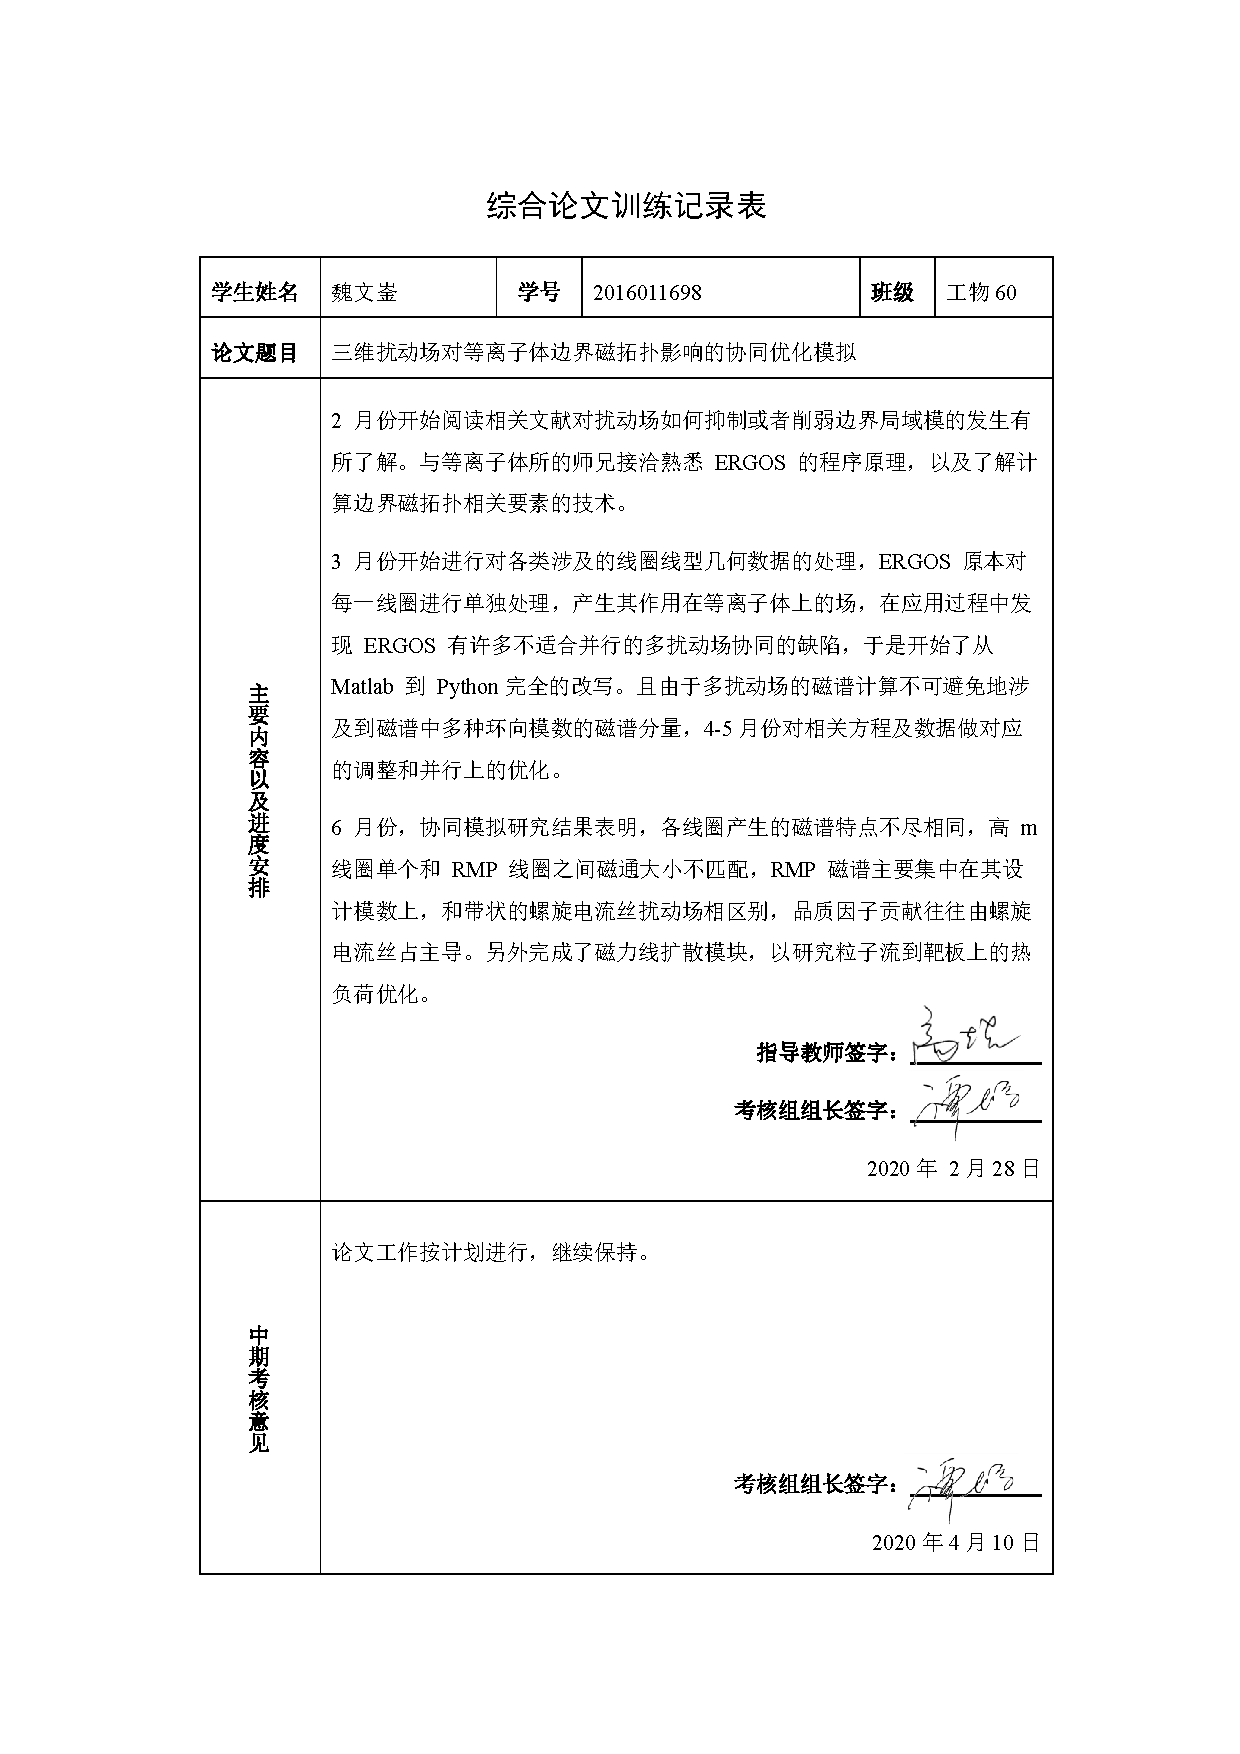
\includepdf[pages=-]{scan-record.pdf}
\end{document}
